\documentclass[11pt]{article}

\usepackage[margin=1in]{geometry}
\usepackage{booktabs}
\usepackage{tabularx}
\usepackage{hyperref}
\usepackage{parskip}
\usepackage{amsmath}
\usepackage{amssymb}
\usepackage{extarrows}
\usepackage{tikz}
\usetikzlibrary{positioning, arrows.meta, calc, decorations.pathreplacing, decorations.pathmorphing, fit, backgrounds}

\setlength{\emergencystretch}{1em}

\newcommand{\excursus}[2]{%
  \begin{center}
  \begin{tikzpicture}
    \node[draw=blue!40, fill=blue!4, rounded corners=4pt,
          inner sep=10pt, text width=0.88\textwidth, font=\small]
    {\textbf{#1}\;\;---\;\;#2};
  \end{tikzpicture}
  \end{center}}

\hypersetup{
  colorlinks=true,
  linkcolor=blue,
  urlcolor=blue,
  citecolor=blue
}

\title{Real-Time Web Communication Standards:\\A Retrospective and Projection\\2021--2031}
\author{}
\date{March 2026}

\begin{document}
\maketitle

\tableofcontents
\listoffigures
\listoftables
\newpage

\section*{Executive Summary}
\addcontentsline{toc}{section}{Executive Summary}

\begin{itemize}
  \item \textbf{Late 2021:} Only WebRTC was a finalized standard with broad
    browser support, and even it had major cross-browser gaps (Safari: H.264
    only, no simulcast, broken iOS DataChannel). QUIC was newly standardized
    but not universal. HTTP/3 was pre-RFC. WebTransport was non-functional.
    WebCodecs existed in one browser. MoQ did not exist.

  \item \textbf{March 2026:} The core stack (WebRTC, QUIC, HTTP/3) is
    standardized and universal. WebCodecs is cross-browser with 94\% coverage.
    Two gaps remain: Safari lacks WebTransport (82\% coverage) and Encoded
    Transforms for E2EE remain Chrome-only.

  \item \textbf{2028--2029 projection:} WebTransport reaches Safari via
    Interop~2026. Encoded Transforms become cross-browser. WebCodecs achieves
    W3C Recommendation. AV1 becomes a practical WebRTC codec as hardware
    encoding expands. MoQ and RTP over QUIC reach RFC status.

  \item \textbf{2029--2031 projection:} Full stack convergence. The
    ``unbundled'' architecture (WebTransport + WebCodecs + WebAssembly) becomes
    viable for specialized use cases. AV1 hardware encoding is ubiquitous.
    MoQ enables standards-based sub-second streaming with CDN fan-out.

  \item \textbf{Hardware and network:} Standards maturation compounds with
    hardware improvement (60--80\% CPU gains vs.\ 2021, ubiquitous AV1 silicon)
    and network growth (200--300~Mbps fixed, 100+~Mbps mobile). By 2030, a
    720p call consumes less than 0.5\% of link capacity.

  \item \textbf{Information-theoretic view (Appendix~\ref{app:info-theory}):}
    Codec efficiency gaps narrow from H.264 ($\Delta \approx 2.1$) to AV1
    ($\Delta \approx 0.4$), approaching the Shannon rate-distortion bound.
    QUIC eliminates head-of-line blocking, recovering up to 34\% per-stream
    throughput at 5\% loss. WebTransport's unreliable datagrams outperform
    WebSocket for any application with a freshness half-life below 34~ms.
\end{itemize}

\section{Introduction}

This document examines the concrete browser capabilities enabled by the
real-time web communication standards collected in the \texttt{standards/}
directory of this project. It compares what these standards made possible in
browsers as of late 2021 with what they enable as of March 2026, then projects
where the stack is heading through 2031. The discussion focuses exclusively on
what standards adoption in browsers enabled and will enable --- not on market
trends, product adoption, or commercial developments.

The standards under review span five areas:
\begin{itemize}
  \item \textbf{WebRTC} --- W3C WebRTC 1.0 and supporting IETF protocols
    (RFCs 8829, 8445, 8826, 8827, 3550, 3711)
  \item \textbf{QUIC} --- RFC 9000
  \item \textbf{HTTP/3} --- RFC 9114
  \item \textbf{WebTransport} --- W3C Working Draft and RFC 9297
  \item \textbf{WebCodecs} --- W3C Working Draft
\end{itemize}

Together, these standards define a full stack for real-time communication in
the browser: from low-level transport (QUIC) through application-layer
protocols (HTTP/3, WebTransport) to peer-to-peer media and data exchange
(WebRTC) and direct codec access (WebCodecs).

Sections~3--7 detail each standard's browser capabilities in late 2021 and
March 2026. Sections~8--9 project the stack's evolution through 2031, grounded
in active W3C charter milestones, IETF draft timelines, browser vendor
signals, and hardware and network trends. Section~10 summarizes the full
2021--2031 trajectory. Appendix~\ref{app:info-theory} applies
information-theoretic measures to quantify channel capacity, source coding
efficiency, and effective information rates across the same time horizons.

Section~2 first provides a concise overview of what each standard does and how
the pieces fit together, for readers unfamiliar with the protocol landscape.

\section{The Standards Stack}
\label{sec:standards-stack}

The standards under review form a layered architecture built on two
complementary transport paths---one \emph{peer-to-peer} (browser talks
directly to browser) and one \emph{client-server} (browser talks to a
server)---with a shared codec layer that bridges both.  This section explains
what each standard does, what problem it solves, and how the pieces fit
together.  Figure~\ref{fig:protocol-stack} provides a visual map; the
subsections below walk through each layer from the bottom up.

\begin{figure}[ht]
\centering
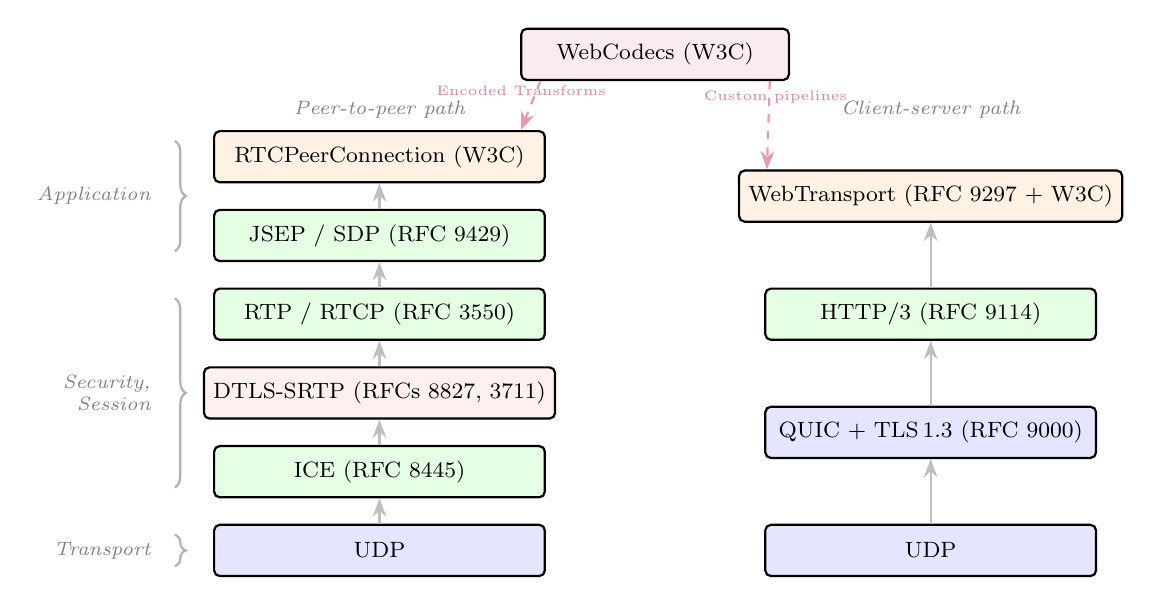
\begin{tikzpicture}[
  >=Stealth,
  block/.style={draw, rounded corners=2pt, minimum height=0.65cm,
    align=center, font=\footnotesize, thick},
  transport/.style={block, fill=blue!10},
  security/.style={block, fill=red!6},
  session/.style={block, fill=green!10},
  app/.style={block, fill=orange!10},
  codec/.style={block, fill=purple!8},
  lbl/.style={font=\scriptsize\itshape, text=black!50},
  arr/.style={->, thick, gray!50},
]

% --- WebRTC side (left) ---
\node[lbl] at (-3.5, 5.6) {Peer-to-peer path};

\node[transport, minimum width=4.2cm] (udp1) at (-3.5, 0) {UDP};
\node[session, minimum width=4.2cm]   (ice)  at (-3.5, 1.0) {ICE (RFC 8445)};
\node[security, minimum width=4.2cm]  (dtls) at (-3.5, 2.0) {DTLS-SRTP (RFCs 8827, 3711)};
\node[session, minimum width=4.2cm]   (rtp)  at (-3.5, 3.0) {RTP / RTCP (RFC 3550)};
\node[session, minimum width=4.2cm]   (jsep) at (-3.5, 4.0) {JSEP / SDP (RFC 9429)};
\node[app, minimum width=4.2cm]       (rtc)  at (-3.5, 5.0) {RTCPeerConnection (W3C)};

% --- QUIC side (right) ---
\node[lbl] at (3.5, 5.6) {Client-server path};

\node[transport, minimum width=4.2cm] (udp2) at (3.5, 0) {UDP};
\node[transport, minimum width=4.2cm] (quic) at (3.5, 1.5) {QUIC + TLS\,1.3 (RFC 9000)};
\node[session, minimum width=4.2cm]   (h3)   at (3.5, 3.0) {HTTP/3 (RFC 9114)};
\node[app, minimum width=4.2cm]       (wt)   at (3.5, 4.5) {WebTransport (RFC 9297 + W3C)};

% --- WebCodecs (centre, spanning both) ---
\node[codec, minimum width=3.4cm] (wc) at (0, 6.3) {WebCodecs (W3C)};

% --- Vertical arrows (WebRTC) ---
\draw[arr] (udp1) -- (ice);
\draw[arr] (ice)  -- (dtls);
\draw[arr] (dtls) -- (rtp);
\draw[arr] (rtp)  -- (jsep);
\draw[arr] (jsep) -- (rtc);

% --- Vertical arrows (QUIC) ---
\draw[arr] (udp2) -- (quic);
\draw[arr] (quic) -- (h3);
\draw[arr] (h3)   -- (wt);

% --- WebCodecs connections (dashed) ---
\draw[->, thick, purple!40, dashed]
  ($(wc.south west)!0.15!(wc.south)$) -- ($(rtc.north east)!0.15!(rtc.north)$);
\draw[->, thick, purple!40, dashed]
  ($(wc.south east)!0.15!(wc.south)$) -- ($(wt.north west)!0.15!(wt.north)$);

\node[font=\tiny, text=purple!50, anchor=south east] at (-0.5, 5.65)
  {Encoded Transforms};
\node[font=\tiny, text=purple!50, anchor=south west] at (0.5, 5.55)
  {Custom pipelines};

% --- Layer annotations (far left) ---
\draw[decorate, decoration={brace, amplitude=4pt, mirror},
  thick, black!30] (-6.1, -0.2) -- (-6.1, 0.2)
  node[midway, left=5pt, lbl] {Transport};
\draw[decorate, decoration={brace, amplitude=4pt, mirror},
  thick, black!30] (-6.1, 0.8) -- (-6.1, 3.2)
  node[midway, left=5pt, lbl, align=right] {Security,\\Session};
\draw[decorate, decoration={brace, amplitude=4pt, mirror},
  thick, black!30] (-6.1, 3.8) -- (-6.1, 5.2)
  node[midway, left=5pt, lbl] {Application};

\end{tikzpicture}
\caption{Protocol stack for the real-time web communication standards.
  Left: the WebRTC peer-to-peer path.  Right: the QUIC-based client-server
  path.  WebCodecs (top centre) provides frame-level codec access regardless
  of transport.}
\label{fig:protocol-stack}
\end{figure}

\subsection{The Underlying Transport: UDP}

All the real-time protocols discussed here ultimately send their data over
\textbf{UDP (User Datagram Protocol)}.  UDP is intentionally simple: it
sends individual packets (called \emph{datagrams}) from one machine to
another with no guarantees about ordering, delivery, or retransmission.  If a
packet is lost, UDP does not notice and does not resend it.

This might seem like a poor foundation, but for real-time media it is
actually an advantage.  In a video call, a video frame that arrives 200~ms
late is useless---the moment it was needed has already passed.  The
alternative, \textbf{TCP (Transmission Control Protocol)}, guarantees that
every byte arrives in order by automatically retransmitting lost packets, but
this creates a problem called \emph{head-of-line blocking}: while TCP waits
for a lost packet to be retransmitted, it holds up delivery of all
subsequent data, even data for completely independent streams.  For
interactive media, this stalling is worse than simply dropping the lost
packet and moving on.  UDP lets the protocols built on top of it make their
own choices about what to retransmit and what to discard.

\subsection{WebRTC: Peer-to-Peer Media in the Browser}

\textbf{WebRTC (Web Real-Time Communication)} is a W3C standard that gives
browsers a built-in ability to send audio, video, and arbitrary data directly
from one browser to another---peer-to-peer, without routing media through a
server.  The browser exposes this through a single JavaScript API called
\texttt{RTCPeerConnection}.  Under the hood, \texttt{RTCPeerConnection}
orchestrates a set of IETF protocols that handle four problems:
\emph{finding a network path} between two peers, \emph{agreeing what media
to send}, \emph{encrypting the media}, and \emph{actually carrying it}.
The subsections below explain each problem and the protocol that solves it.

\subsubsection{Finding a Path: ICE, STUN, and TURN}

The first problem is deceptively hard.  Most devices on the internet do not
have their own public IP address.  Instead, they sit behind a
\textbf{NAT (Network Address Translator)}---typically the home router or
corporate firewall---which assigns the device a \emph{private} address
(like \texttt{192.168.1.x}) and translates outgoing traffic onto a single
\emph{public} address that is visible to the rest of the internet.  This
means two browsers behind different NATs cannot simply send packets to each
other: neither knows the other's routable address, and even if it did, the
receiving NAT would likely drop the unsolicited incoming packet.

WebRTC solves this with \textbf{ICE (Interactive Connectivity Establishment,
RFC~8445)}.  ICE is not a server---it is an algorithm that runs in each
browser, systematically searching for a working network path between two
peers.  The search uses two types of infrastructure servers:

\begin{description}
  \item[STUN (Session Traversal Utilities for NAT)] is a lightweight,
    stateless server that serves one purpose: when a browser sends it a
    request, the STUN server replies with the browser's \emph{public} IP
    address and port---the address as seen from the far side of the NAT.
    This is called a \emph{server-reflexive candidate}: the browser now knows
    what address the outside world sees for it.  The STUN server relays no
    media and maintains no per-session state; it simply reflects the
    address back.

  \item[TURN (Traversal Using Relays around NAT)] is a heavier-weight server
    used as a last resort.  When two peers are both behind restrictive NATs
    (such as corporate firewalls that block all unsolicited inbound traffic),
    no direct path exists between them.  In this case, both peers connect to a
    TURN server, which allocates ports, authenticates each peer, and
    \emph{relays} all media packets between them for the duration of the
    session.  This works through any NAT because both peers are making
    outbound connections to the TURN server.  The cost is that all media flows
    through the relay, adding latency and bandwidth consumption.
    Approximately 10--20\% of WebRTC connections require TURN.
\end{description}

The ICE process works as follows.  Each browser gathers a set of
\emph{candidates}---potential addresses through which it might be
reachable:

\begin{enumerate}
  \item \textbf{Host candidates:} the device's own local IP addresses
    (useful when both peers are on the same local network).
  \item \textbf{Server-reflexive candidates:} the public address discovered
    via STUN (useful when the NAT allows direct traffic once the mapping is
    known).
  \item \textbf{Relay candidates:} a port allocated on a TURN server
    (the guaranteed fallback).
\end{enumerate}

Both peers exchange their candidate lists (via the signaling mechanism
described below), and ICE constructs every possible pairing of one local
candidate with one remote candidate.  It then tests each pair in priority
order---host pairs first (lowest latency), then server-reflexive pairs, then
relay pairs---by sending a probe and waiting for a response.  The first pair
that works is selected, and media begins flowing over it.

\textbf{Trickle ICE (RFC~8838)} improves this process by allowing candidates
to be exchanged and tested incrementally, as they are discovered, rather
than waiting for the full list to be compiled.  In practice, this reduces
connection setup time to roughly 500--800~ms because the fastest candidates
(host and server-reflexive) are typically discovered and tested within the
first few hundred milliseconds.

\begin{figure}[ht]
\centering
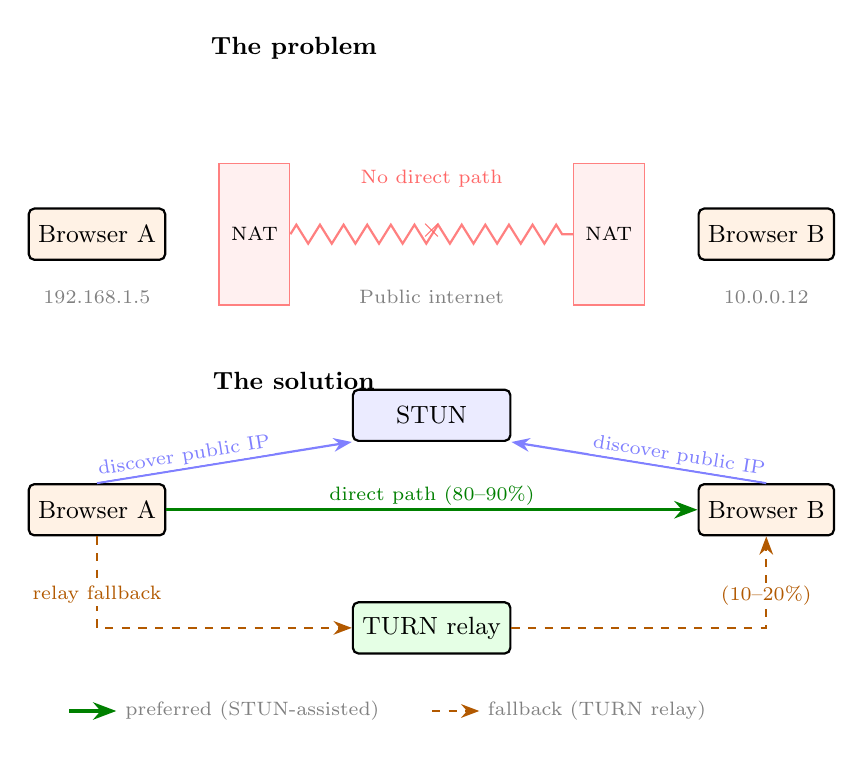
\begin{tikzpicture}[
  >=Stealth,
  peer/.style={rectangle, draw, rounded corners=2pt, fill=orange!10,
    minimum width=1.6cm, minimum height=0.65cm, font=\small, thick},
  nat/.style={rectangle, draw=red!50, fill=red!6,
    minimum width=0.9cm, minimum height=1.8cm,
    font=\scriptsize, align=center},
  server/.style={rectangle, draw, rounded corners=2pt, fill=#1,
    minimum width=2cm, minimum height=0.65cm, font=\small, thick},
  server/.default={blue!8},
  arr/.style={->, thick, #1},
  arr/.default={black!60},
  darr/.style={->, thick, dashed, #1},
  darr/.default={black!60},
  lbl/.style={font=\scriptsize, fill=white, inner sep=1pt},
]

% --- Left: The NAT problem ---
\node[font=\small\bfseries, anchor=south] at (2.5, 3.6) {The problem};

\node[peer] (pA) at (0, 1.5) {Browser A};
\node[nat]  (nA) at (2, 1.5) {NAT};
\node[nat]  (nB) at (6.5, 1.5) {NAT};
\node[peer] (pB) at (8.5, 1.5) {Browser B};

\node[font=\scriptsize, text=gray] at (0, 0.7) {192.168.1.5};
\node[font=\scriptsize, text=gray] at (8.5, 0.7) {10.0.0.12};

\draw[thick, red!50, decorate,
  decoration={zigzag, segment length=3mm, amplitude=1.2mm}]
  (nA.east) -- (nB.west);
\node[font=\normalsize\bfseries, text=red!60] at (4.25, 1.55) {$\times$};
\node[font=\scriptsize, text=red!60] at (4.25, 2.2) {No direct path};
\node[font=\scriptsize, text=gray] at (4.25, 0.7) {Public internet};

% --- Right: The solution ---
\node[font=\small\bfseries, anchor=south] at (2.5, -0.6) {The solution};

\node[peer] (pA2) at (0, -2) {Browser A};
\node[peer] (pB2) at (8.5, -2) {Browser B};
\node[server=blue!8] (stun) at (4.25, -0.8) {STUN};
\node[server=green!10] (turn) at (4.25, -3.5) {TURN relay};

% STUN arrows
\draw[arr=blue!50] (pA2.north) -- node[lbl, above, sloped, pos=0.35]
  {\scriptsize discover public IP} (stun.south west);
\draw[arr=blue!50] (pB2.north) -- node[lbl, above, sloped, pos=0.35]
  {\scriptsize discover public IP} (stun.south east);

% Direct path (80-90%)
\draw[arr=green!50!black, line width=1.2pt] (pA2.east) --
  node[lbl, above] {\scriptsize direct path (80--90\%)} (pB2.west);

% TURN fallback (10-20%)
\draw[darr=orange!70!black] (pA2.south) |-
  node[lbl, below, pos=0.25] {\scriptsize relay fallback} (turn.west);
\draw[darr=orange!70!black] (turn.east) -|
  node[lbl, below, pos=0.75] {\scriptsize (10--20\%)} (pB2.south);

% Legend
\node[font=\scriptsize, text=gray, align=left, anchor=north west]
  at (-0.5, -4.3) {%
  \tikz[baseline=-0.5ex]{\draw[->, thick, green!50!black, line width=1.2pt]
    (0,0) -- (0.6,0);}~preferred (STUN-assisted) \qquad
  \tikz[baseline=-0.5ex]{\draw[->, thick, dashed, orange!70!black]
    (0,0) -- (0.6,0);}~fallback (TURN relay)};

\end{tikzpicture}
\caption{The NAT problem and how ICE solves it.  Top: two browsers behind
  NATs cannot reach each other directly---neither knows the other's public
  address.  Bottom: STUN discovers each browser's public address; ICE
  attempts a direct connection (successful 80--90\% of the time) and falls
  back to a TURN relay when direct connectivity is impossible.}
\label{fig:nat-ice}
\end{figure}

\subsubsection{Agreeing What to Send: SDP, JSEP, and Signaling}

Before media can flow, two peers must agree on what they will send each
other: which codecs to use (H.264, VP9, AV1), which media types (audio,
video, screen-share), at what resolutions and bitrates, and which encryption
parameters.  This negotiation uses the \textbf{Session Description Protocol
(SDP)}---a text-based format that describes a peer's media capabilities.

The process works through an \emph{offer/answer} exchange:
\begin{enumerate}
  \item \textbf{Peer~A creates an SDP offer} listing everything it can send
    and receive: ``I support H.264 and VP9 video, Opus audio, and here is my
    encryption certificate fingerprint.''
  \item \textbf{The offer is delivered to Peer~B} through a signaling
    channel.
  \item \textbf{Peer~B creates an SDP answer} selecting the common ground:
    ``I also support VP9 and Opus; let's use those.  Here is my encryption
    fingerprint.''
  \item \textbf{The answer is delivered back to Peer~A.}  Both peers now know
    exactly what media they will exchange and how it will be encrypted.
\end{enumerate}

\textbf{JSEP (JavaScript Session Establishment Protocol, RFC~9429;
originally RFC~8829)} defines how the browser creates and processes these
SDP messages.  It specifies the JavaScript API calls---\texttt{createOffer()},
\texttt{createAnswer()}, \texttt{setLocalDescription()},
\texttt{setRemoteDescription()}---that applications use to drive the
negotiation.

Critically, JSEP \emph{deliberately does not specify how} the SDP offer and
answer are delivered between the two peers.  This delivery mechanism is
called \textbf{signaling}, and it is the one part of a WebRTC system that
the application must build itself.  The signaling channel can be anything:
a WebSocket connection, an HTTP request, a message passed through a shared
database---whatever gets the SDP text from one peer to the other.  The
signaling server also relays ICE candidates as they are discovered (for
Trickle ICE).  Importantly, the signaling server never sees or touches the
actual media; it handles only lightweight control messages.

\subsubsection{Encrypting the Media: DTLS and SRTP}

All WebRTC media is encrypted.  There is no option to send unencrypted
audio or video---encryption is mandatory by design.

The encryption uses two protocols working together:

\begin{description}
  \item[DTLS (Datagram Transport Layer Security, RFC~8827)] is essentially
    TLS (the same encryption used for HTTPS websites) adapted for UDP.  Once
    ICE has found a working path between two peers, DTLS performs a
    cryptographic handshake over that path.  During the handshake, each peer
    presents a self-signed certificate, and the remote peer verifies that the
    certificate matches the fingerprint it received earlier in the SDP
    exchange.  This binding between the signaling channel and the media
    channel prevents \emph{man-in-the-middle attacks}: an attacker cannot
    substitute their own encryption keys without the mismatch being detected.
    The DTLS handshake produces a shared set of encryption keys.

  \item[SRTP (Secure Real-time Transport Protocol, RFC~3711)] uses the keys
    negotiated by DTLS to encrypt every individual media packet.  SRTP adds
    a small authentication tag to each packet (a few bytes), enabling the
    receiver to verify that the packet has not been tampered with in transit.
    The overhead is negligible and introduces no meaningful latency.
\end{description}

\subsubsection{Carrying the Media: RTP and RTCP}

With a path established (ICE), capabilities agreed (SDP/JSEP), and
encryption keys negotiated (DTLS), media can finally flow.  The protocol
that carries the actual audio and video is \textbf{RTP (Real-time Transport
Protocol, RFC~3550)}, sent as encrypted SRTP packets.

RTP provides the essential bookkeeping for real-time media:
\begin{itemize}
  \item \textbf{Sequence numbers} so the receiver can detect lost packets
    and reorder packets that arrive out of sequence.
  \item \textbf{Timestamps} so the receiver can synchronize audio and video
    playback (lip sync) and play back frames at the correct rate.
  \item \textbf{Payload type identifiers} so the receiver knows which codec
    was used to encode each packet.
\end{itemize}

Alongside RTP, the \textbf{RTP Control Protocol (RTCP)} provides a feedback
channel.  Receivers periodically send RTCP reports back to the sender with
statistics on packet loss rate, jitter (variation in packet arrival times),
and round-trip time.  The sender uses this feedback to adapt in real time:
if packet loss increases, the video encoder can reduce its bitrate to avoid
further congestion.  This adaptive behaviour is essential for maintaining
call quality over varying network conditions.

\subsubsection{The WebRTC Security Model}

RFC~8826 defines the overarching security principles for WebRTC:
\begin{itemize}
  \item \textbf{Mandatory encryption:} as described above, all media is
    encrypted via DTLS-SRTP.
  \item \textbf{User consent:} the browser must obtain explicit user
    permission before accessing the camera or microphone.  A web page cannot
    silently record audio or video.
  \item \textbf{IP address privacy:} browsers use \textbf{mDNS (multicast
    DNS)} to mask local IP addresses in ICE candidates.  Without this,
    a web page could discover the user's local network address merely by
    initiating a WebRTC connection, creating a privacy leak.  With mDNS,
    the browser substitutes a random hostname that resolves only on the
    local network.
\end{itemize}

\subsubsection{Putting It Together: A WebRTC Call Sequence}

Figure~\ref{fig:webrtc-sequence} illustrates the end-to-end sequence.
When a user joins a video call:

\begin{enumerate}
  \item The browser gathers ICE candidates (local addresses, STUN-discovered
    public addresses, and optionally TURN relay addresses).
  \item The application creates an SDP offer describing the browser's media
    capabilities and sends it, along with the ICE candidates, through the
    signaling server to the remote peer.
  \item The remote peer responds with an SDP answer and its own ICE
    candidates.
  \item ICE tests candidate pairs and selects the best working path.
  \item DTLS performs a handshake over that path to negotiate encryption
    keys.
  \item Encrypted media (audio and video as SRTP packets) begins flowing
    directly between the two browsers.  The signaling server is no longer
    in the media path.
\end{enumerate}

\begin{figure}[ht]
\centering
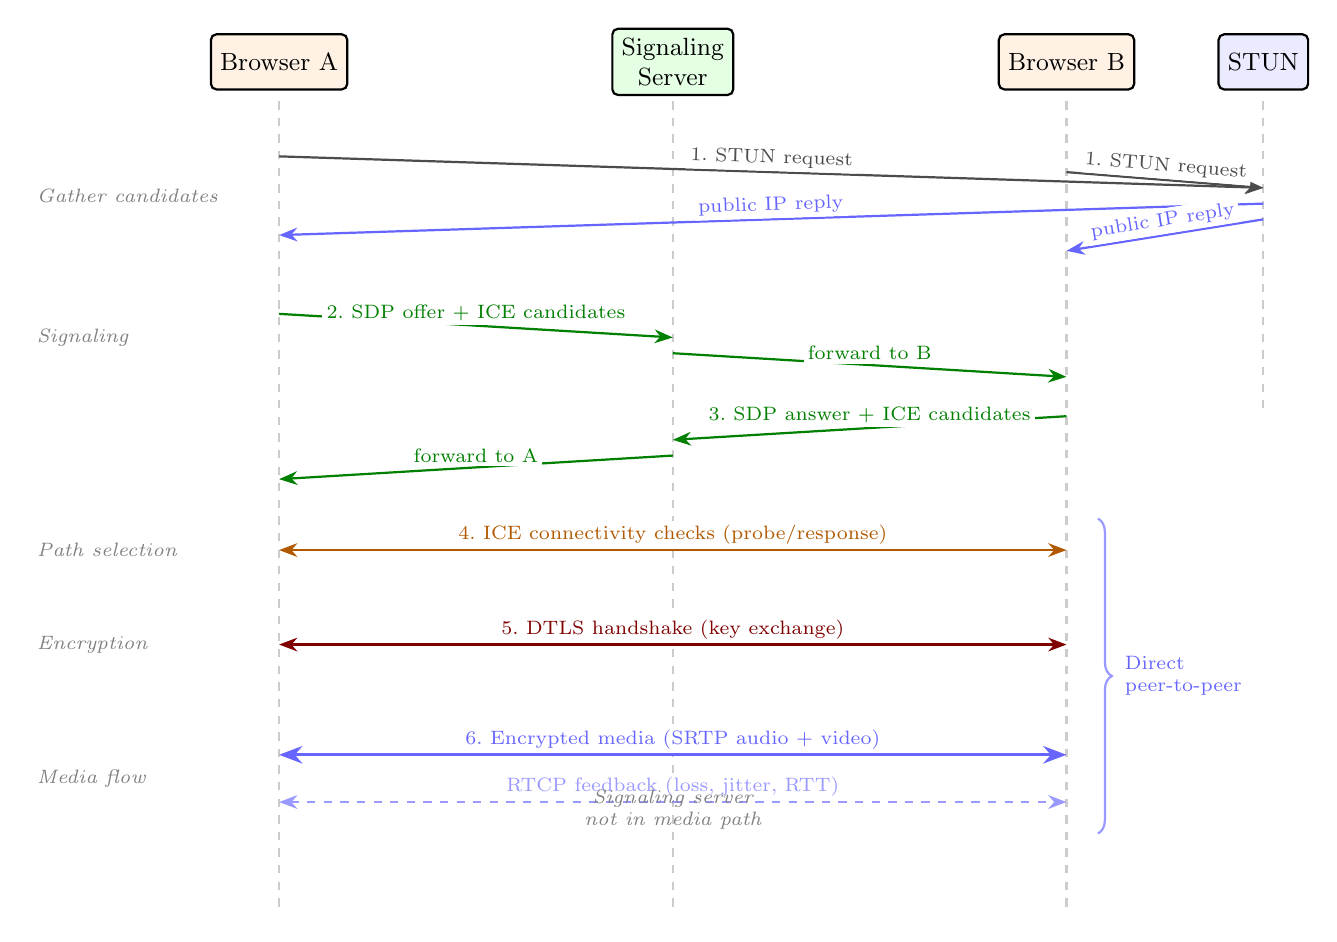
\begin{tikzpicture}[
  >=Stealth,
  entity/.style={rectangle, draw, rounded corners=2pt, minimum height=0.7cm,
    align=center, font=\small, thick, fill=#1},
  entity/.default={white},
  msg/.style={->, thick, #1},
  msg/.default={black!70},
  mlbl/.style={font=\scriptsize, fill=white, inner sep=1.5pt},
  timeline/.style={thick, gray!40, dashed},
]

% --- Entities ---
\node[entity=orange!10] (peerA) at (0, 0)    {Browser A};
\node[entity=green!10]  (sig)   at (5, 0)    {Signaling\\Server};
\node[entity=orange!10] (peerB) at (10, 0)   {Browser B};
\node[entity=blue!8]    (stun)  at (12.5, 0) {STUN};

% --- Timelines ---
\draw[timeline] (0, -0.5) -- (0, -10.8);
\draw[timeline] (5, -0.5) -- (5, -10.8);
\draw[timeline] (10, -0.5) -- (10, -10.8);
\draw[timeline] (12.5, -0.5) -- (12.5, -4.5);

% --- Step 1: STUN discovery ---
\draw[msg] (0, -1.2) -- node[mlbl, above, sloped]
  {1.\ STUN request} (12.5, -1.6);
\draw[msg=blue!60] (12.5, -1.8) -- node[mlbl, above, sloped]
  {public IP reply} (0, -2.2);
\draw[msg] (10, -1.4) -- node[mlbl, above, sloped]
  {1.\ STUN request} (12.5, -1.6);
\draw[msg=blue!60] (12.5, -2.0) -- node[mlbl, above, sloped]
  {public IP reply} (10, -2.4);

\node[font=\scriptsize\itshape, text=black!50, anchor=west] at (-3.2, -1.7)
  {Gather candidates};

% --- Step 2: SDP offer + candidates ---
\draw[msg=green!50!black] (0, -3.2) -- node[mlbl, above]
  {2.\ SDP offer + ICE candidates} (5, -3.5);
\draw[msg=green!50!black] (5, -3.7) -- node[mlbl, above]
  {forward to B} (10, -4.0);

\node[font=\scriptsize\itshape, text=black!50, anchor=west] at (-3.2, -3.5)
  {Signaling};

% --- Step 3: SDP answer + candidates ---
\draw[msg=green!50!black] (10, -4.5) -- node[mlbl, above]
  {3.\ SDP answer + ICE candidates} (5, -4.8);
\draw[msg=green!50!black] (5, -5.0) -- node[mlbl, above]
  {forward to A} (0, -5.3);

% --- Step 4: ICE connectivity checks ---
\draw[msg=orange!70!black, <->] (0, -6.2) -- node[mlbl, above]
  {4.\ ICE connectivity checks (probe/response)} (10, -6.2);

\node[font=\scriptsize\itshape, text=black!50, anchor=west] at (-3.2, -6.2)
  {Path selection};

% --- Step 5: DTLS handshake ---
\draw[msg=red!50!black, <->] (0, -7.4) -- node[mlbl, above]
  {5.\ DTLS handshake (key exchange)} (10, -7.4);

\node[font=\scriptsize\itshape, text=black!50, anchor=west] at (-3.2, -7.4)
  {Encryption};

% --- Step 6: Media flow ---
\draw[msg=blue!60, <->, line width=1.2pt] (0, -8.8) -- node[mlbl, above]
  {6.\ Encrypted media (SRTP audio + video)} (10, -8.8);
\draw[msg=blue!40, <->, dashed] (0, -9.4) -- node[mlbl, above]
  {RTCP feedback (loss, jitter, RTT)} (10, -9.4);

\node[font=\scriptsize\itshape, text=black!50, anchor=west] at (-3.2, -9.1)
  {Media flow};

% --- Signaling server not in media path ---
\node[font=\scriptsize\itshape, text=gray, align=center] at (5, -9.5)
  {Signaling server\\not in media path};

% Brace for direct peer-to-peer
\draw[decorate, decoration={brace, amplitude=5pt},
  thick, blue!40] (10.4, -5.8) -- (10.4, -9.8)
  node[midway, right=6pt, font=\scriptsize, text=blue!60, align=left]
  {Direct\\peer-to-peer};

\end{tikzpicture}
\caption{WebRTC call establishment sequence.  Steps~1--3 use supporting
  infrastructure (STUN server, signaling server).  Once ICE selects a path
  and DTLS establishes encryption (steps~4--5), media flows directly between
  the two browsers (step~6).  The signaling server plays no further role
  in the media path.}
\label{fig:webrtc-sequence}
\end{figure}

\subsection{QUIC: A Modern Transport Protocol}

\textbf{QUIC (RFC~9000)} is a general-purpose transport protocol that, like
WebRTC's media path, runs over UDP.  It was originally developed by Google
and standardized by the IETF in 2021.  QUIC is designed to solve several
long-standing problems with TCP, the transport protocol that has carried most
internet traffic for decades.

\textbf{The head-of-line blocking problem.}  TCP provides a single,
ordered byte stream: every byte must be delivered in sequence.  When a
browser opens multiple parallel data flows over one TCP connection (as
HTTP/2 does), a single lost packet blocks \emph{all} of those flows until
the lost packet is retransmitted and received.  This is head-of-line
blocking.  QUIC solves it by providing \emph{many independent streams}
within a single connection, each with its own sequencing and flow control.
A lost packet on one stream stalls only that stream; all others continue
unaffected.  For applications carrying multiple concurrent flows---such as
a video call with several media tracks---this independence is critical.

\begin{figure}[ht]
\centering
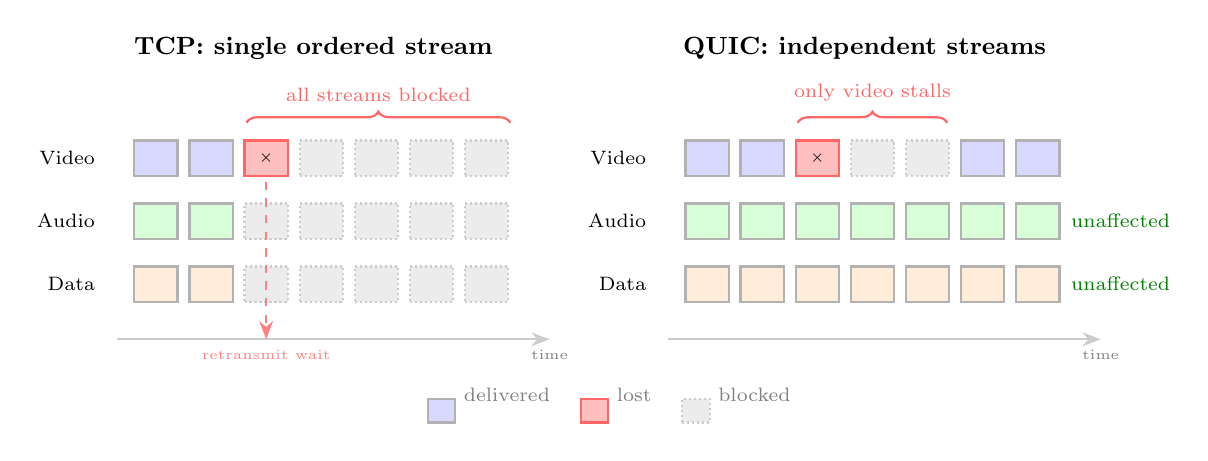
\begin{tikzpicture}[
  >=Stealth,
  pkt/.style={minimum width=0.55cm, minimum height=0.45cm,
    font=\tiny, align=center, thick, draw},
  lost/.style={pkt, fill=red!25, draw=red!60},
  ok/.style={pkt, fill=#1, draw=gray!60},
  ok/.default={blue!15},
  blocked/.style={pkt, fill=gray!15, draw=gray!40, densely dotted},
  lbl/.style={font=\scriptsize},
  heading/.style={font=\small\bfseries},
]

% === TCP side (left) ===
\node[heading] at (2.5, 3.6) {TCP: single ordered stream};

% Stream labels
\node[lbl, anchor=east] at (-0.15, 2.2) {Video};
\node[lbl, anchor=east] at (-0.15, 1.4) {Audio};
\node[lbl, anchor=east] at (-0.15, 0.6) {Data};

% Timeline arrow
\draw[->, thick, gray!40] (0, -0.1) -- (5.5, -0.1)
  node[anchor=north, font=\tiny, text=gray] {time};

% Video packets
\node[ok=blue!15] at (0.5, 2.2) {};
\node[ok=blue!15] at (1.2, 2.2) {};
\node[lost] at (1.9, 2.2) {\bfseries $\times$};
\node[blocked] at (2.6, 2.2) {};
\node[blocked] at (3.3, 2.2) {};
\node[blocked] at (4.0, 2.2) {};
\node[blocked] at (4.7, 2.2) {};

% Audio packets
\node[ok=green!15] at (0.5, 1.4) {};
\node[ok=green!15] at (1.2, 1.4) {};
\node[blocked] at (1.9, 1.4) {};
\node[blocked] at (2.6, 1.4) {};
\node[blocked] at (3.3, 1.4) {};
\node[blocked] at (4.0, 1.4) {};
\node[blocked] at (4.7, 1.4) {};

% Data packets
\node[ok=orange!15] at (0.5, 0.6) {};
\node[ok=orange!15] at (1.2, 0.6) {};
\node[blocked] at (1.9, 0.6) {};
\node[blocked] at (2.6, 0.6) {};
\node[blocked] at (3.3, 0.6) {};
\node[blocked] at (4.0, 0.6) {};
\node[blocked] at (4.7, 0.6) {};

% Blocked annotation
\draw[thick, red!60, decorate,
  decoration={brace, amplitude=4pt}]
  (1.65, 2.65) -- (5.0, 2.65)
  node[midway, above=4pt, font=\scriptsize, text=red!60]
  {all streams blocked};

% Retransmit annotation
\draw[->, thick, red!50, dashed] (1.9, 1.9) -- (1.9, -0.1)
  node[anchor=north, font=\tiny, text=red!50] {retransmit wait};

% === QUIC side (right) ===
\node[heading] at (9.5, 3.6) {QUIC: independent streams};

\node[lbl, anchor=east] at (6.85, 2.2) {Video};
\node[lbl, anchor=east] at (6.85, 1.4) {Audio};
\node[lbl, anchor=east] at (6.85, 0.6) {Data};

% Timeline arrow
\draw[->, thick, gray!40] (7, -0.1) -- (12.5, -0.1)
  node[anchor=north, font=\tiny, text=gray] {time};

% Video packets - one lost, only video stalls
\node[ok=blue!15] at (7.5, 2.2) {};
\node[ok=blue!15] at (8.2, 2.2) {};
\node[lost] at (8.9, 2.2) {\bfseries $\times$};
\node[blocked] at (9.6, 2.2) {};
\node[blocked] at (10.3, 2.2) {};
\node[ok=blue!15] at (11.0, 2.2) {};
\node[ok=blue!15] at (11.7, 2.2) {};

% Audio packets - unaffected
\node[ok=green!15] at (7.5, 1.4) {};
\node[ok=green!15] at (8.2, 1.4) {};
\node[ok=green!15] at (8.9, 1.4) {};
\node[ok=green!15] at (9.6, 1.4) {};
\node[ok=green!15] at (10.3, 1.4) {};
\node[ok=green!15] at (11.0, 1.4) {};
\node[ok=green!15] at (11.7, 1.4) {};

% Data packets - unaffected
\node[ok=orange!15] at (7.5, 0.6) {};
\node[ok=orange!15] at (8.2, 0.6) {};
\node[ok=orange!15] at (8.9, 0.6) {};
\node[ok=orange!15] at (9.6, 0.6) {};
\node[ok=orange!15] at (10.3, 0.6) {};
\node[ok=orange!15] at (11.0, 0.6) {};
\node[ok=orange!15] at (11.7, 0.6) {};

% Only video stalls annotation
\draw[thick, red!60, decorate,
  decoration={brace, amplitude=4pt}]
  (8.65, 2.65) -- (10.55, 2.65)
  node[midway, above=4pt, font=\scriptsize, text=red!60]
  {only video stalls};

\node[font=\scriptsize, text=green!50!black, anchor=west] at (12, 1.4)
  {unaffected};
\node[font=\scriptsize, text=green!50!black, anchor=west] at (12, 0.6)
  {unaffected};

% Legend
\node[font=\scriptsize, text=gray, anchor=north] at (6.25, -0.6) {%
  \tikz[baseline=-0.5ex]{\node[ok=blue!15, minimum width=0.35cm,
    minimum height=0.3cm] {};}~delivered \quad
  \tikz[baseline=-0.5ex]{\node[lost, minimum width=0.35cm,
    minimum height=0.3cm] {};}~lost \quad
  \tikz[baseline=-0.5ex]{\node[blocked, minimum width=0.35cm,
    minimum height=0.3cm] {};}~blocked};

\end{tikzpicture}
\caption{Head-of-line blocking: TCP vs.\ QUIC.  Left: when a TCP packet is
  lost, \emph{all} multiplexed streams stall until the lost packet is
  retransmitted.  Right: QUIC isolates the loss to the affected stream;
  audio and data continue flowing without interruption.}
\label{fig:hol-blocking-concept}
\end{figure}

\textbf{Built-in encryption.}  QUIC integrates TLS~1.3 (Transport Layer
Security, the same encryption standard used for HTTPS) directly into the
connection handshake.  A new QUIC connection is established in a single
network round trip (1-RTT), compared to TCP's three-way handshake followed
by a separate TLS handshake (typically 2--3 round trips).  For servers the
client has previously connected to, QUIC can establish a connection with
\emph{zero} round trips (0-RTT), sending application data in the very first
packet.

\textbf{Connection migration.}  Traditional TCP connections are identified
by a \emph{5-tuple}: source IP address, source port, destination IP address,
destination port, and protocol number.  When any of these change---for
example, when a phone switches from Wi-Fi to cellular---the TCP connection
breaks and must be re-established.  QUIC instead identifies connections by
\emph{connection IDs}, opaque tokens that survive network changes.  When a
device changes networks, QUIC validates the new path and continues the
session without interruption.  For a video call, this means seamless handoff
rather than a disconnect-and-reconnect.

\subsection{HTTP/3: HTTP over QUIC}

\textbf{HTTP/3 (RFC~9114)} is the latest version of the HTTP protocol that
powers the web.  It maps HTTP requests and responses onto QUIC instead of
TCP.  Each HTTP request/response pair occupies its own QUIC stream, so the
head-of-line blocking that affects HTTP/2 (which multiplexes over a single
TCP connection) is eliminated: a lost packet delays only the request it
belongs to, not every other request on the connection.

For the standards discussed in this document, HTTP/3 matters primarily
because it is the foundation on which WebTransport is built.  A
WebTransport session is established over an HTTP/3 connection, inheriting
all of QUIC's properties: independent streams, built-in encryption,
connection migration, and low-latency connection establishment.

\subsection{WebTransport: QUIC Capabilities for Browser Applications}

\textbf{WebTransport (W3C Working Draft + RFC~9297)} is a browser API that
gives JavaScript applications direct access to QUIC's transport capabilities
over an HTTP/3 connection.  To understand why this matters, consider the
alternative: \textbf{WebSocket}.

WebSocket, the current standard for bidirectional browser-server
communication, runs over TCP.  It provides a single ordered byte stream---
the same model as a regular TCP connection, with the same head-of-line
blocking problem.  If a WebSocket sends a burst of small messages and one
packet is lost, all subsequent messages stall until the lost one is
retransmitted.  Furthermore, every message sent over WebSocket is guaranteed
to arrive (TCP will retransmit until it does), even if the message has become
stale by the time it finally arrives.

WebTransport offers three capabilities that WebSocket cannot:

\begin{itemize}
  \item \textbf{Unreliable datagrams.}  An application can send a message
    that is delivered if possible but silently dropped if lost.  No
    retransmission, no stalling.  This is ideal for data that becomes stale
    quickly---game state updates, real-time cursor positions, live sensor
    readings---where receiving the \emph{latest} value matters more than
    receiving \emph{every} value.

  \item \textbf{Multiple independent reliable streams.}  An application can
    open many parallel streams, each with guaranteed in-order delivery, but
    without head-of-line blocking between them.  A stall on one stream does
    not affect the others.  This is useful for sending different types of
    data (e.g., chat messages, control signals, file transfers)
    simultaneously without interference.

  \item \textbf{Connection migration.}  Inherited from QUIC: the
    connection survives network changes such as Wi-Fi to cellular handoffs.
\end{itemize}

\begin{figure}[ht]
\centering
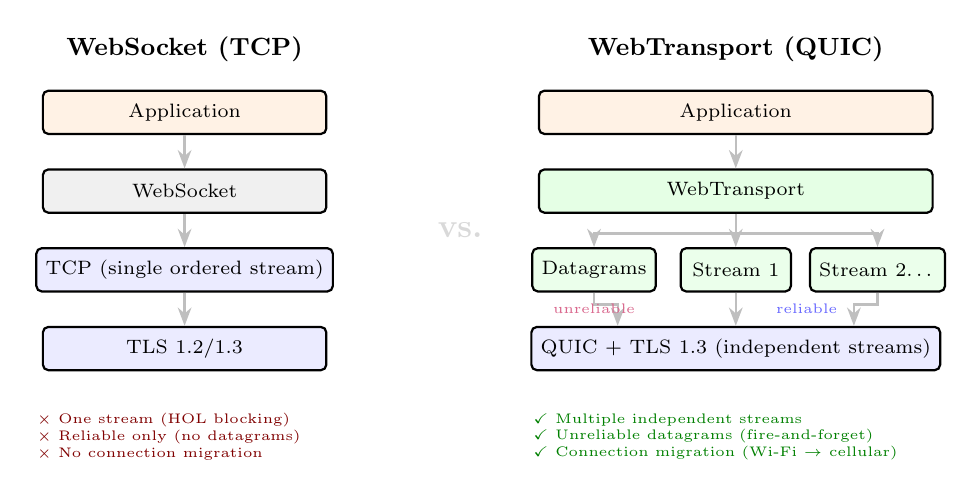
\begin{tikzpicture}[
  >=Stealth,
  block/.style={draw, rounded corners=2pt, minimum height=0.55cm,
    align=center, font=\scriptsize, thick},
  heading/.style={font=\small\bfseries},
  arr/.style={->, thick, gray!50},
  lbl/.style={font=\tiny, text=gray},
]

% === WebSocket side (left) ===
\node[heading] at (2.0, 4.0) {WebSocket (TCP)};

\node[block, fill=orange!10, minimum width=3.6cm] (wsApp) at (2.0, 3.2)
  {Application};
\node[block, fill=gray!12, minimum width=3.6cm] (ws) at (2.0, 2.2)
  {WebSocket};
\node[block, fill=blue!8, minimum width=3.6cm] (tcp) at (2.0, 1.2)
  {TCP (single ordered stream)};
\node[block, fill=blue!8, minimum width=3.6cm] (tls) at (2.0, 0.2)
  {TLS 1.2/1.3};

\draw[arr] (wsApp) -- (ws);
\draw[arr] (ws) -- (tcp);
\draw[arr] (tcp) -- (tls);

% Limitations
\node[font=\tiny, text=red!50!black, anchor=north west, align=left]
  at (0.0, -0.5) {%
  $\times$ One stream (HOL blocking)\\
  $\times$ Reliable only (no datagrams)\\
  $\times$ No connection migration};

% === WebTransport side (right) ===
\node[heading] at (9.0, 4.0) {WebTransport (QUIC)};

\node[block, fill=orange!10, minimum width=5.0cm] (wtApp) at (9.0, 3.2)
  {Application};
\node[block, fill=green!10, minimum width=5.0cm] (wt2) at (9.0, 2.2)
  {WebTransport};

% Three capabilities
\node[block, fill=green!8, minimum width=1.4cm] (dg) at (7.2, 1.2)
  {Datagrams};
\node[block, fill=green!8, minimum width=1.4cm] (s1) at (9.0, 1.2)
  {Stream 1};
\node[block, fill=green!8, minimum width=1.4cm] (s2) at (10.8, 1.2)
  {Stream 2\ldots};

\node[block, fill=blue!8, minimum width=5.0cm] (quic2) at (9.0, 0.2)
  {QUIC + TLS 1.3 (independent streams)};

\draw[arr] (wtApp) -- (wt2);
\draw[arr] (wt2.south) -- ++(0, -0.25) -| (dg.north);
\draw[arr] (wt2.south) -- ++(0, -0.25) -| (s1.north);
\draw[arr] (wt2.south) -- ++(0, -0.25) -| (s2.north);
\draw[arr] (dg.south) -- ++(0, -0.15) -| ([xshift=-1.5cm]quic2.north);
\draw[arr] (s1) -- (quic2);
\draw[arr] (s2.south) -- ++(0, -0.15) -| ([xshift=1.5cm]quic2.north);

% Advantages
\node[font=\tiny, text=green!50!black, anchor=north west, align=left]
  at (6.3, -0.5) {%
  \checkmark{} Multiple independent streams\\
  \checkmark{} Unreliable datagrams (fire-and-forget)\\
  \checkmark{} Connection migration (Wi-Fi $\to$ cellular)};

% Label on datagrams
\node[font=\tiny, text=purple!60] at (7.2, 0.7) {unreliable};
\node[font=\tiny, text=blue!60] at (9.9, 0.7) {reliable};

% VS divider
\node[font=\large\bfseries, text=gray!30] at (5.5, 1.7) {vs.};

\end{tikzpicture}
\caption{WebSocket vs.\ WebTransport.  WebSocket provides a single ordered
  stream over TCP; a lost packet stalls everything.  WebTransport provides
  multiple independent streams \emph{and} unreliable datagrams over QUIC,
  with connection migration.}
\label{fig:ws-vs-wt}
\end{figure}

WebTransport is a \emph{client-server} protocol: the browser connects to a
server, not directly to another browser.  It complements WebRTC---where
WebRTC provides direct browser-to-browser media exchange, WebTransport
provides a modern browser-to-server data path suited to relayed media
architectures, game state synchronization, and real-time telemetry.

\subsection{WebCodecs: Direct Codec Access}

\textbf{WebCodecs (W3C Working Draft)} gives JavaScript code direct,
frame-by-frame access to the audio and video codecs built into the browser.

To understand why this matters, consider how browsers have traditionally
handled media encoding and decoding.  High-level APIs like
\texttt{MediaRecorder} (for recording) and \texttt{HTMLMediaElement} (for
playback) control the entire pipeline: the browser decides when to produce
keyframes, how to adjust bitrate, and what container format to use.  The
application gets a finished recording or a rendered video---but cannot
intervene at the level of individual frames.

WebCodecs breaks open this pipeline.  It provides four interfaces:

\begin{itemize}
  \item \texttt{VideoEncoder} / \texttt{VideoDecoder} --- encode or decode
    individual video frames, with per-frame control over keyframe insertion,
    target bitrate, and quality parameters.
  \item \texttt{AudioEncoder} / \texttt{AudioDecoder} --- the same for
    individual audio chunks.
\end{itemize}

These interfaces use the browser's built-in hardware-accelerated codec
implementations.  When dedicated encoding hardware is available (as on most
modern GPUs and mobile chips), WebCodecs uses it automatically; otherwise it
falls back to software encoding.  The application gets raw encoded bytes
without container overhead, and can process, transform, or transport them
however it chooses.

WebCodecs is deliberately \emph{transport-agnostic}---it handles encoding
and decoding, not delivery.  The encoded output can be sent via WebRTC (using
Encoded Transforms to insert custom processing into the
\texttt{RTCPeerConnection} pipeline), via WebTransport (packaging encoded
frames as datagrams or stream data), or via any other mechanism.

\begin{figure}[ht]
\centering
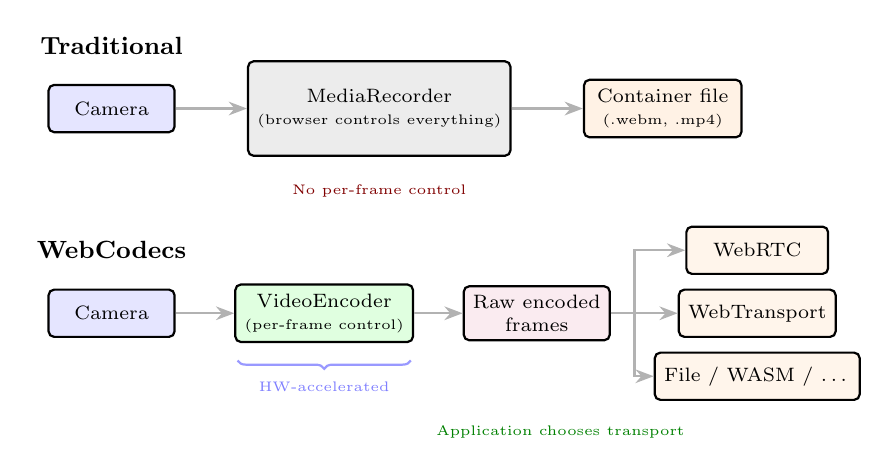
\begin{tikzpicture}[
  >=Stealth,
  block/.style={draw, rounded corners=2pt, minimum height=0.6cm,
    align=center, font=\scriptsize, thick},
  heading/.style={font=\small\bfseries},
  arr/.style={->, thick, gray!60},
  lbl/.style={font=\tiny, text=gray},
]

% === Traditional path (top) ===
\node[heading] at (0.8, 2.4) {Traditional};

\node[block, fill=blue!10, minimum width=1.6cm] (cam1) at (0.8, 1.6)
  {Camera};
\node[block, fill=gray!15, minimum width=3.2cm, minimum height=1.2cm]
  (mr) at (4.2, 1.6)
  {MediaRecorder\\{\tiny(browser controls everything)}};
\node[block, fill=orange!10, minimum width=2.0cm] (out1) at (7.8, 1.6)
  {Container file\\{\tiny(.webm, .mp4)}};

\draw[arr] (cam1) -- (mr);
\draw[arr] (mr) -- (out1);

\node[font=\tiny, text=red!50!black, anchor=north] at (4.2, 0.75)
  {No per-frame control};

% === WebCodecs path (bottom) ===
\node[heading] at (0.8, -0.2) {WebCodecs};

\node[block, fill=blue!10, minimum width=1.6cm] (cam2) at (0.8, -1.0)
  {Camera};
\node[block, fill=green!12, minimum width=2.0cm] (ve) at (3.5, -1.0)
  {VideoEncoder\\{\tiny(per-frame control)}};
\node[block, fill=purple!8, minimum width=1.6cm] (raw) at (6.2, -1.0)
  {Raw encoded\\frames};

% Multiple output paths
\node[block, fill=orange!8, minimum width=1.8cm] (rtc2) at (9.0, -0.2)
  {WebRTC};
\node[block, fill=orange!8, minimum width=1.8cm] (wt3) at (9.0, -1.0)
  {WebTransport};
\node[block, fill=orange!8, minimum width=1.8cm] (other) at (9.0, -1.8)
  {File / WASM / \ldots};

\draw[arr] (cam2) -- (ve);
\draw[arr] (ve) -- (raw);
\draw[arr] (raw.east) -- ++(0.3, 0) |- (rtc2.west);
\draw[arr] (raw) -- (wt3);
\draw[arr] (raw.east) -- ++(0.3, 0) |- (other.west);

\node[font=\tiny, text=green!50!black, anchor=north] at (6.5, -2.3)
  {Application chooses transport};

% Brace for HW accel
\draw[decorate, decoration={brace, amplitude=3pt, mirror},
  thick, blue!40] (2.4, -1.6) -- (4.6, -1.6)
  node[midway, below=4pt, font=\tiny, text=blue!50] {HW-accelerated};

\end{tikzpicture}
\caption{Traditional codec access vs.\ WebCodecs.  Top: \texttt{MediaRecorder}
  controls the entire pipeline; the application receives a finished container
  file.  Bottom: WebCodecs gives per-frame control over hardware-accelerated
  encoding, and the application decides how to transport the raw output.}
\label{fig:webcodecs-pipeline}
\end{figure}

\subsection{How the Standards Interact}

The standards described above can be summarized in four key relationships:

\begin{enumerate}
  \item \textbf{WebRTC is self-contained for peer-to-peer communication.}
    A single API call, \texttt{RTCPeerConnection}, bundles ICE (path
    discovery), DTLS-SRTP (encryption), RTP (media transport), and codec
    negotiation.  An application can build a complete video call using only
    WebRTC and an application-provided signaling channel, without touching
    any other standard discussed here.

  \item \textbf{QUIC $\to$ HTTP/3 $\to$ WebTransport is a layered
    client-server path.}  Each layer adds capability: QUIC provides
    multiplexed encrypted transport over UDP, HTTP/3 maps HTTP semantics
    onto it, and WebTransport exposes QUIC's streams and datagrams to
    JavaScript.  An application that needs browser-to-server real-time
    communication uses all three layers, but interacts only with the
    WebTransport API at the top.

  \item \textbf{WebCodecs bridges both paths.}  In a WebRTC context,
    WebCodecs (via Encoded Transforms) enables custom processing of media
    frames flowing through \texttt{RTCPeerConnection}---for example,
    applying end-to-end encryption inside the WebRTC pipeline.  In a
    WebTransport context, WebCodecs encodes and decodes media that the
    application transports itself, independent of WebRTC.

  \item \textbf{The ``unbundled'' alternative.}  Rather than using WebRTC's
    monolithic \texttt{RTCPeerConnection}, an application can compose
    WebTransport (for transport) + WebCodecs (for encoding/decoding) +
    WebAssembly (for custom processing) to build a fully custom media
    pipeline.  This trades WebRTC's built-in integration for explicit control
    over every decision: which codec, what packetization, how to handle
    congestion, what to retransmit.  This architecture is projected to become
    viable by 2029 (Sections~8--9).
\end{enumerate}

\section{WebRTC}

The WebRTC stack in the \texttt{standards/} directory comprises the W3C
WebRTC 1.0 specification and six IETF RFCs: JSEP (RFC~8829), ICE
(RFC~8445), the WebRTC security considerations (RFC~8826), the DTLS-based
security architecture (RFC~8827), RTP (RFC~3550), and SRTP (RFC~3711).

\subsection{Late 2021}

W3C WebRTC 1.0 achieved Recommendation status in January 2021, making it a
finalized standard. By late 2021, Chrome and Firefox offered full
implementations, and Edge inherited Chrome's support via its Chromium base.
Safari supported the core API but with significant limitations:

\begin{itemize}
  \item \textbf{Codec restrictions.} Safari supported only H.264 for video.
    Chrome and Firefox supported VP8, VP9, and H.264. This meant Safari could
    not participate in VP9-based calls and lacked access to VP9's more
    efficient bandwidth usage.
  \item \textbf{No simulcast or SVC.} Safari could not send multiple
    encodings of the same video stream at different resolutions (simulcast)
    or use Scalable Video Coding (SVC). Chrome and Firefox supported both,
    enabling adaptive quality based on network conditions.
  \item \textbf{RTCDataChannel issues on iOS.} The data channel did not work
    reliably on iOS Safari. Cross-browser data channel connections between
    Safari on iOS and Chrome or Firefox failed due to missing local ICE
    candidates on iOS.
  \item \textbf{SDP handling divergence.} Chrome was in the process of
    migrating from Plan~B to Unified Plan SDP semantics. Chrome~M89
    (February 2021) added deprecation warnings; Chrome~M93 (August 2021)
    removed Plan~B with a reverse origin trial option. Firefox and Safari
    already used Unified Plan exclusively. During this transition, applications
    had to accommodate both SDP formats.
  \item \textbf{Insertable Streams.} Chrome~M94 introduced the
    Insertable Streams API, enabling JavaScript to access and transform
    encoded media frames in the WebRTC pipeline. This was essential for
    end-to-end encryption of media. Firefox and Safari did not implement it.
  \item \textbf{Stats reporting inconsistencies.} Firefox was missing
    \texttt{voice\-Activity\-Flag} on video track stats. Safari was missing
    \texttt{rtpTimestamp} and \texttt{voiceActivityFlag}. Applications could
    not reliably detect voice activity or obtain precise timing information
    across browsers.
\end{itemize}

On the IETF side, the supporting protocols were in the following state:
\begin{itemize}
  \item \textbf{JSEP (RFC~8829)} was published in January 2021 alongside the
    W3C Recommendation. All browsers implemented the JSEP signaling
    state machine through \texttt{RTCPeerConnection}, but diverged in areas
    like BUNDLE handling of multiple media streams.
  \item \textbf{ICE (RFC~8445)} was implemented in all browsers. Trickle ICE
    (RFC~8838), enabling incremental candidate exchange rather than waiting for
    full gathering, was published in January 2021 but not yet mandatory.
  \item \textbf{DTLS-SRTP (RFCs~8827, 3711)} was mandatory across all
    browsers. All media was encrypted. However, browsers differed in DTLS
    certificate algorithms (Chrome~52+ used ECDSA; others varied), and
    privacy identifier reset mechanisms were inconsistent.
  \item \textbf{Security (RFC~8826)} --- all browsers enforced
    camera/microphone permission prompts and encrypted all media. However,
    protections against IP address leakage were inconsistent; not all browsers
    masked local IP addresses via mDNS candidates when media permissions had
    not been granted.
\end{itemize}

\subsection{March 2026}

The W3C updated the WebRTC 1.0 Recommendation in October 2024 and again in
2025, incorporating amendments based on implementation experience.

\begin{itemize}
  \item \textbf{Unified Plan is universal.} Plan~B SDP is completely removed
    from all browsers. Applications no longer need to accommodate both formats.
  \item \textbf{Safari gained VP9.} Safari~15 and later support the VP9 codec
    for WebRTC, enabling Safari to participate in VP9-based calls and benefit
    from VP9's bandwidth efficiency. Safari still prefers H.264 for hardware
    acceleration, and its SVC support remains limited compared to
    Chrome and Firefox.
  \item \textbf{iOS WebRTC matured.} Starting with iOS~14.3, WebRTC works
    reliably across all browsers on iOS. RTCDataChannel connections between
    iOS Safari and desktop Chrome or Firefox are reliable.
  \item \textbf{JSEP updated to RFC~9429.} Published in April 2024, RFC~9429
    obsoleted RFC~8829, addressing implementation divergence --- particularly
    in BUNDLE handling and bundle-only \texttt{m=} sections.
  \item \textbf{Trickle ICE is mandatory.} All browsers implement RFC~8838,
    enabling faster connection establishment through incremental candidate
    exchange.
  \item \textbf{mDNS privacy protections standardized.} Chrome, Firefox, and
    Safari all mask local IP addresses using mDNS candidates when
    camera/microphone permissions have not been granted, implementing the
    privacy considerations of RFC~8826.
  \item \textbf{Encoded Transforms remain Chrome-only.} The feature
    evolved from ``Insertable Streams'' to \texttt{RTCRtp\-Script\-Transform}
    (WebRTC Encoded Transform), but Firefox and Safari still do not
    implement it. End-to-end encryption of encoded media frames in the
    WebRTC pipeline remains a Chrome/Chromium-only capability.
\end{itemize}

\section{QUIC}

RFC~9000 defines the QUIC transport protocol: a UDP-based, multiplexed,
encrypted transport with built-in TLS~1.3, independent stream flow control,
and connection migration across network changes.

\subsection{Late 2021}

RFC~9000 was published in May 2021. Browser support was uneven:

\begin{itemize}
  \item \textbf{Chrome} had QUIC enabled by default, having been an early
    adopter (Google developed the original QUIC protocol).
  \item \textbf{Firefox~88} (April 2021) enabled QUIC by default.
  \item \textbf{Safari} had experimental QUIC support (added in Safari
    Technology Preview~104, April 2020), but it required manual opt-in
    through experimental settings. It was not available to ordinary users.
\end{itemize}

In practice, a browser connecting to a QUIC-capable server would benefit from
reduced connection latency (0-RTT or 1-RTT handshakes vs.\ TCP's multi-round
handshake plus TLS), elimination of head-of-line blocking across multiplexed
streams, and connection survival across network changes. But with Safari
requiring manual opt-in, these benefits were unavailable to most Safari users.

\subsection{March 2026}

QUIC is enabled by default in all major browsers:
\begin{itemize}
  \item Chrome, Edge, and Firefox continue default support.
  \item Safari~16 (2022) enabled QUIC by default, bringing universal coverage.
\end{itemize}

Every major browser can now establish QUIC connections transparently. The
capabilities defined by RFC~9000 --- low-latency connection establishment,
multiplexed streams without head-of-line blocking, built-in encryption, and
connection migration --- are universally available to web applications without
any user or developer opt-in.

\section{HTTP/3}

RFC~9114 maps HTTP semantics over QUIC, inheriting QUIC's transport
properties: multiplexed streams without head-of-line blocking, lower
connection latency, and connection migration.

\subsection{Late 2021}

RFC~9114 had not yet been published (it was finalized in June 2022). Browsers
were shipping pre-standard HTTP/3 implementations based on draft
specifications:

\begin{itemize}
  \item \textbf{Chrome} had experimental HTTP/3 support enabled by default
    since April 2020.
  \item \textbf{Firefox~88} (April 2021) enabled HTTP/3 by default.
  \item \textbf{Safari} had HTTP/3 support behind an experimental feature
    flag, disabled by default.
\end{itemize}

Where supported, browsers could negotiate HTTP/3 with compatible servers,
gaining per-stream independence (a stalled stream would not block other
streams, unlike HTTP/2 over TCP). However, the lack of a finalized RFC meant
implementations were based on draft specifications that could diverge, and
Safari's experimental-only status limited universal availability.

\subsection{March 2026}

With RFC~9114 finalized in June 2022, all major browsers now support HTTP/3
by default:
\begin{itemize}
  \item Chrome, Edge, and Firefox have supported HTTP/3 by default for
    several years.
  \item Safari enabled HTTP/3 by default starting with Safari~16 (2022).
  \item Over 92\% of browser market share supports HTTP/3.
\end{itemize}

The capabilities defined by RFC~9114 --- HTTP request/response multiplexing
without head-of-line blocking, lower latency connection establishment via
QUIC, and connection resilience across network changes --- are now universally
available. Any browser connecting to an HTTP/3-capable server automatically
benefits from these properties.

\section{WebTransport}

The WebTransport specification defines browser APIs for bidirectional
client-server communication over HTTP/3, supporting both reliable streams and
unreliable datagrams. RFC~9297 defines the HTTP datagram and capsule protocol
mechanisms that underpin it.

\subsection{Late 2021}

WebTransport was in a very early state:

\begin{itemize}
  \item \textbf{Chrome} had experimental support but it was disabled in
    Chrome~M91 through M94. The API was not usable in production.
  \item \textbf{Firefox} had no support whatsoever.
  \item \textbf{Safari} had no support whatsoever.
  \item RFC~9297 had not yet been published (August 2022).
  \item The W3C specification was an early Working Draft.
\end{itemize}

In late 2021, WebTransport was effectively unavailable in any browser for
production use. The capabilities it defines --- unreliable datagrams from
browser to server, multiple independent reliable streams, and connection
migration --- could not be used by web applications.

\subsection{March 2026}

WebTransport has achieved broad but not universal support:

\begin{itemize}
  \item \textbf{Chrome~97+} and \textbf{Edge~98+} support WebTransport
    (stable since late 2021 / early 2022).
  \item \textbf{Firefox~114+} (2023) supports WebTransport.
  \item \textbf{Safari does not support WebTransport.}
  \item Approximately 82\% of browser market share has WebTransport support.
\end{itemize}

For browsers that support it, WebTransport enables capabilities that were
previously impossible without WebRTC's peer-to-peer architecture:
\begin{itemize}
  \item \textbf{Unreliable datagrams} from browser to server, suitable for
    latency-sensitive data where retransmission is undesirable (e.g., game
    state updates, real-time sensor data).
  \item \textbf{Multiple independent reliable streams} without head-of-line
    blocking between them, enabling parallel data flows over a single
    connection.
  \item \textbf{Connection migration} across network changes, inherited from
    QUIC.
\end{itemize}

Safari's absence means applications using WebTransport must provide fallback
mechanisms (typically WebSocket) for Safari users, or accept that these
capabilities are unavailable on Apple platforms.

\section{WebCodecs}

The WebCodecs specification provides JavaScript interfaces for direct access
to the browser's built-in audio, video, and image codecs, enabling
frame-level encoding and decoding outside of higher-level APIs like
\texttt{MediaRecorder} or \texttt{HTMLMediaElement}.

\subsection{Late 2021}

WebCodecs had just reached initial availability:

\begin{itemize}
  \item \textbf{Chrome~94} (September 2021) shipped WebCodecs as a stable
    feature, graduating from origin trial. Chrome~92 and 93 had offered it
    as an origin trial with breaking changes between versions.
  \item \textbf{Firefox} had no support.
  \item \textbf{Safari} had no support.
  \item The W3C specification was a First Public Working Draft (2021).
\end{itemize}

In Chrome~94, developers could for the first time:
\begin{itemize}
  \item Encode and decode individual video frames using
    \texttt{VideoEncoder} and \texttt{VideoDecoder} with the browser's
    hardware-accelerated codecs, without being constrained by
    \texttt{MediaRecorder}'s real-time recording model.
  \item Encode and decode individual audio chunks
    (\texttt{AudioEncoder}/\texttt{AudioDecoder}).
  \item Perform faster-than-realtime encoding (previously impossible via
    \texttt{MediaRecorder}).
  \item Control per-frame keyframe insertion and quality parameters.
  \item Obtain raw encoded bytes without container overhead.
\end{itemize}

However, these capabilities were Chrome-only. Firefox and Safari users had no
access to low-level codec APIs; they were limited to the high-level
\texttt{MediaRecorder} and \texttt{HTMLMediaElement} interfaces.

\subsection{March 2026}

WebCodecs has achieved broad cross-browser support:

\begin{itemize}
  \item \textbf{Chrome/Edge} --- supported since version 94 (2021).
  \item \textbf{Firefox~130+} (September 2024) --- shipped approximately three
    years after Chrome.
  \item \textbf{Safari~26+} (2024) --- full support. Earlier Safari versions
    (16.4+) had partial video-only support.
  \item Approximately 94\% of browser market share supports WebCodecs.
  \item The specification remains a W3C Working Draft (updated January 2026),
    not yet a Recommendation.
\end{itemize}

With cross-browser support, all major browsers can now perform frame-level
codec operations using hardware acceleration. This enables web applications
to build custom media pipelines --- video editors, live transcoders, custom
streaming clients --- that were previously possible only through WebAssembly
codec implementations or native applications.

\section{Looking Ahead: 2028--2029 (Two to Three Years)}

The following projections are grounded in active W3C charter milestones, IETF
draft publication timelines, and formal browser vendor implementation signals.

\subsection{WebCodecs Reaches W3C Recommendation}

The W3C Media Working Group charter targets WebCodecs Candidate
Recommendation in Q1~2026 and full Recommendation by Q4~2026. By 2028, the
specification should be a mature, finalized standard. This means the
frame-level codec access that was Chrome-only in 2021 and cross-browser by
2026 will have a stable, locked-down API surface that browser vendors commit
to maintaining long-term. The WebCodecs Codec Registry will likely include
formal AV1 registration entries alongside existing H.264, VP8, and VP9
entries.

\subsection{WebTransport Achieves Universal Browser Support}

Apple committed WebTransport as a formal Interop~2026 priority, accounting
for 20\% of the interoperability score. Safari already has experimental
WebTransport support behind a flag in iOS~18. Given this commitment, Safari
production support is expected by late 2026 or early 2027, with the W3C
specification reaching Recommendation status around the same time. By 2028,
WebTransport should be universally available across all major browsers ---
closing the last significant gap in the stack. Applications will be able to
rely on browser-to-server unreliable datagrams and independent reliable
streams without Safari fallbacks.

\subsection{WebRTC Encoded Transforms Become Cross-Browser}

The \texttt{RTCRtpScriptTransform} API (WebRTC Encoded Transform) has a
Working Draft dated February 2026 and is approaching Candidate
Recommendation. Safari and Firefox have implemented it natively; Chrome
continues support via its earlier Insertable Streams lineage. By 2028, this
API should be standardized and available across all major browsers, enabling
cross-browser end-to-end encryption of media frames within the WebRTC
pipeline --- a capability that was Chrome-only from 2021 through 2026.

\subsection{AV1 Becomes a Practical WebRTC Codec}

Firefox enabled AV1 for WebRTC by default in 2025. Chrome has supported it
for several years. By 2028, AV1 hardware encoding support in consumer devices
will have expanded, reducing the CPU cost that currently limits its adoption.
AV1's superior compression efficiency (roughly 30\% better than VP9 at
equivalent quality) will make it a practical default codec for WebRTC calls
in Chrome and Firefox. Safari's adoption remains uncertain, as Apple
historically favors H.264 with hardware acceleration.

\subsection{Media over QUIC Reaches RFC Status}

The IETF Media over QUIC (MoQ) transport draft
(\texttt{draft-ietf-moq-transport}) is advancing rapidly, with version~15
published in October 2025. The protocol enables subscription-based media
publishing and consuming over QUIC, designed for low-latency distribution
with CDN support. By 2028, MoQ should have reached RFC status, along with
companion specifications for media container formats (Low Overhead Media
Container) and streaming formats. Browser integration will likely occur
through JavaScript libraries built on WebTransport and WebCodecs rather than
through dedicated browser APIs --- the component APIs are already in place to
support this.

\subsection{RTP over QUIC Reaches RFC Status}

The IETF RTP over QUIC (RoQ) draft (\texttt{draft-ietf-avtcore-rtp-over-quic})
maps RTP and RTCP packets onto QUIC streams and datagrams. By 2028, this
should reach RFC status, enabling WebRTC backends to transport media over
QUIC instead of the traditional UDP+DTLS-SRTP path. Browser-facing
integration would occur through SDP negotiation rather than new JavaScript
APIs, potentially enabling WebRTC calls to benefit from QUIC's congestion
control and connection migration at the transport layer.

\subsection{Hardware and Network Context}

The standards projections above do not exist in a vacuum. By 2028, two
underlying trends amplify what these standards make practically possible.

\textbf{CPU and hardware acceleration.} AV1 encoding is computationally
expensive --- in 2026, real-time AV1 encoding for a WebRTC call can consume
an entire CPU core on mid-range hardware, which is why VP9 and H.264 remain
the practical defaults despite AV1's superior compression. By 2028, dedicated
AV1 hardware encoders will be standard in new laptops, phones, and tablets
(Apple's M-series chips, Qualcomm Snapdragon, Intel Arc, and AMD RDNA
already include or are adding AV1 encode blocks). This shifts AV1 from
``technically supported but too expensive'' to ``hardware-accelerated and
free.'' The WebCodecs API, which exposes hardware-accelerated codecs to
JavaScript, directly benefits: an application calling
\texttt{VideoEncoder} with AV1 in 2028 will hit dedicated silicon rather than
a software encoder, making frame-level AV1 processing via WebCodecs
practical for real-time use cases.

Similarly, the unbundled architecture --- composing WebTransport, WebCodecs,
and WebAssembly --- imposes CPU overhead from JavaScript orchestration and
WebAssembly processing that would have been prohibitive on 2021 hardware.
By 2028, the roughly 40--50\% improvement in single-thread CPU performance
since 2021 (compounding at approximately 8--10\% annually) makes this
overhead manageable for real-time media pipelines.

\textbf{Network bandwidth.} Global median fixed broadband speeds have
approximately doubled from 2021 to 2026 (from roughly 60~Mbps to over
120~Mbps in developed markets), and 5G mobile networks have expanded
substantially. By 2028, continued growth in fixed and mobile bandwidth
means that the efficiency gains from AV1 and QUIC compound with raw
bandwidth increases. A WebRTC call using AV1 over QUIC on a 2028 connection
will have both a more efficient codec (30\% less bandwidth than VP9) and
more available bandwidth, enabling higher resolution and frame rates within
the same network cost envelope. QUIC's connection migration (RFC~9000)
becomes more impactful as mobile usage grows --- a video call that seamlessly
survives a Wi-Fi to 5G handoff requires both the protocol support (already
standardized) and sufficient mobile bandwidth to sustain the call (increasingly
available).

The net effect is that the standards reaching maturity by 2028 will land on
hardware and networks that can fully exploit them, rather than being
bottlenecked by the infrastructure they run on.

\begin{figure}[ht]
\centering
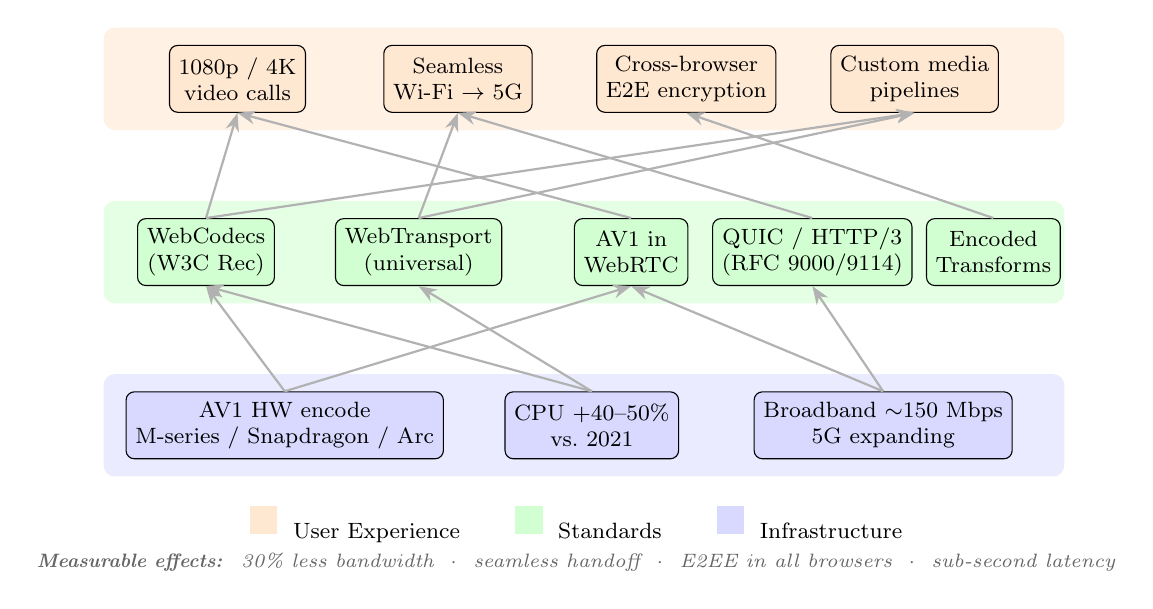
\begin{tikzpicture}[
  >=Stealth,
  item/.style={draw, rounded corners=3pt, minimum height=0.85cm,
    align=center, font=\footnotesize, fill=white},
  arr/.style={->, thick, gray!60},
  metriclabel/.style={font=\scriptsize\itshape, text=black!60},
]

% --- Layer background bands (no border, distinct colors) ---
\fill[blue!8, rounded corners=4pt]
  (-5.5, -0.65) rectangle (6.7, 0.65);
\fill[green!10, rounded corners=4pt]
  (-5.5, 1.55) rectangle (6.7, 2.85);
\fill[orange!10, rounded corners=4pt]
  (-5.5, 3.75) rectangle (6.7, 5.05);

% --- Infrastructure items ---
\node[item, fill=blue!15] (hw) at (-3.2, 0)
  {AV1 HW encode\\M-series / Snapdragon / Arc};
\node[item, fill=blue!15] (cpu) at (0.7, 0)
  {CPU +40--50\%\\vs.\ 2021};
\node[item, fill=blue!15] (net) at (4.4, 0)
  {Broadband ${\sim}$150~Mbps\\5G expanding};

% --- Standards items ---
\node[item, fill=green!18] (wc) at (-4.2, 2.2)
  {WebCodecs\\(W3C Rec)};
\node[item, fill=green!18] (wt) at (-1.5, 2.2)
  {WebTransport\\(universal)};
\node[item, fill=green!18] (av1) at (1.2, 2.2)
  {AV1 in\\WebRTC};
\node[item, fill=green!18] (quic) at (3.5, 2.2)
  {QUIC / HTTP/3\\(RFC 9000/9114)};
\node[item, fill=green!18] (et) at (5.8, 2.2)
  {Encoded\\Transforms};

% --- User experience items ---
\node[item, fill=orange!18] (hd) at (-3.8, 4.4)
  {1080p / 4K\\video calls};
\node[item, fill=orange!18] (handoff) at (-1.0, 4.4)
  {Seamless\\Wi-Fi $\to$ 5G};
\node[item, fill=orange!18] (e2ee) at (1.9, 4.4)
  {Cross-browser\\E2E encryption};
\node[item, fill=orange!18] (custom) at (4.8, 4.4)
  {Custom media\\pipelines};

% --- Arrows: infrastructure -> standards ---
\draw[arr] (hw.north) -- (wc.south);
\draw[arr] (hw.north) -- (av1.south);
\draw[arr] (cpu.north) -- (wt.south);
\draw[arr] (cpu.north) -- (wc.south);
\draw[arr] (net.north) -- (quic.south);
\draw[arr] (net.north) -- (av1.south);

% --- Arrows: standards -> user experience ---
\draw[arr] (wc.north) -- (hd.south);
\draw[arr] (wc.north) -- (custom.south);
\draw[arr] (av1.north) -- (hd.south);
\draw[arr] (wt.north) -- (custom.south);
\draw[arr] (wt.north) -- (handoff.south);
\draw[arr] (quic.north) -- (handoff.south);
\draw[arr] (et.north) -- (e2ee.south);

% --- Legend (below diagram, horizontal) ---
\node[anchor=north, font=\footnotesize] at (0.5, -0.9) {%
  \tikz[baseline=-0.5ex]{\fill[orange!18] (0,0) rectangle (0.35,0.35);}
  ~User Experience \qquad
  \tikz[baseline=-0.5ex]{\fill[green!18] (0,0) rectangle (0.35,0.35);}
  ~Standards \qquad
  \tikz[baseline=-0.5ex]{\fill[blue!15] (0,0) rectangle (0.35,0.35);}
  ~Infrastructure};

% --- Measurable effects ---
\node[metriclabel, anchor=north, align=center] at (0.5, -1.5)
  {\textbf{Measurable effects:} ~30\% less bandwidth
   ~$\cdot$~ seamless handoff ~$\cdot$~
   E2EE in all browsers ~$\cdot$~ sub-second latency};

\end{tikzpicture}
\caption{By 2028: infrastructure enables standards to deliver measurable
  user experience gains. Arrows show enabling relationships.}
\label{fig:2028-stack}
\end{figure}

\section{Looking Ahead: 2029--2031 (Three to Five Years)}

These projections extend further from current standardization activity and
carry correspondingly more uncertainty, but follow from the trajectory
established by the standards work described above.

\subsection{The ``Unbundled'' Architecture Becomes Viable}

By 2029, all the component APIs --- WebTransport (universal), WebCodecs
(Recommendation), and RTCRtpScriptTransform (standardized) --- will have been
stable and cross-browser for two or more years. This makes the ``WebRTC
Unbundled'' architecture practically viable: applications can compose
WebTransport for data transport, WebCodecs for encoding and decoding, and
WebAssembly for custom processing, bypassing the monolithic
\texttt{RTCPeerConnection} API entirely.

This matters because the unbundled approach gives applications control over
decisions that WebRTC currently makes internally: which codec to use, how to
packetize, what transport to use, and how to handle congestion. Use cases
that are poorly served by WebRTC's built-in assumptions --- cloud gaming
requiring ultra-low latency with acceptable loss, scientific visualization
requiring custom frame processing, or broadcast distribution requiring
one-to-many fan-out --- can be built from these composable primitives.

Traditional WebRTC via \texttt{RTCPeerConnection} will persist for general
video conferencing, where its built-in codec negotiation, ICE connectivity,
and DTLS-SRTP security provide a well-integrated default. The unbundled
approach is not a replacement but an alternative for applications with
specialized requirements.

\begin{figure}[ht]
\centering
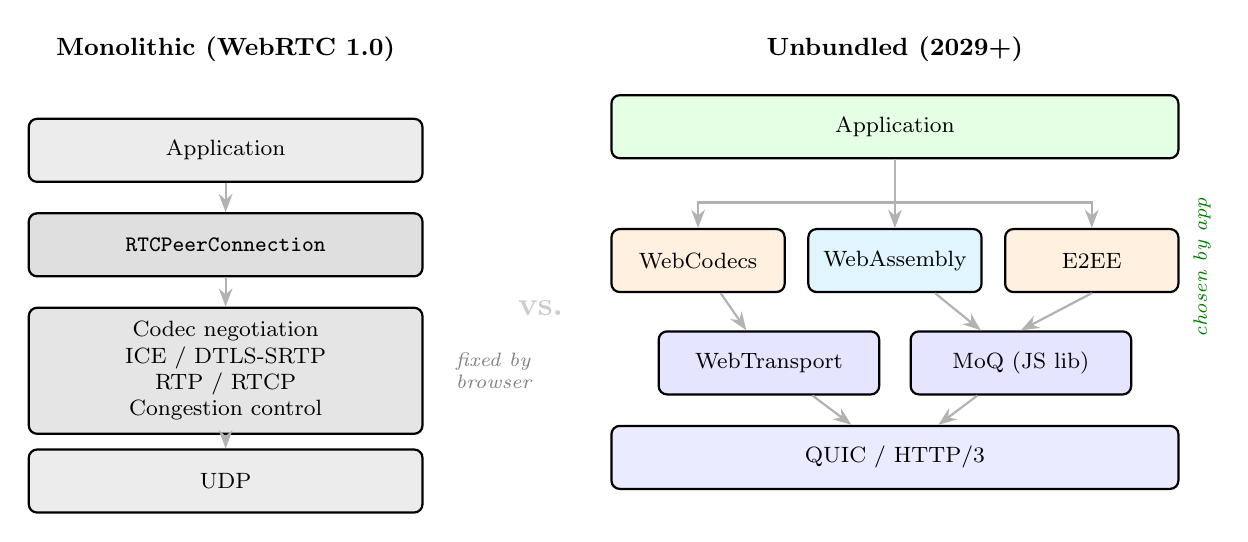
\begin{tikzpicture}[
  >=Stealth,
  block/.style={draw, rounded corners=3pt, minimum height=0.8cm,
    align=center, font=\footnotesize, thick},
  monolith/.style={block, fill=gray!15, minimum width=5cm},
  unbundled/.style={block, fill=green!10, minimum width=2.6cm},
  label/.style={font=\small\bfseries, anchor=south},
  arr/.style={->, thick, gray!60},
  brace/.style={decorate, decoration={brace, amplitude=6pt, mirror}},
]

% --- Monolithic side (left) ---
\node[label] at (-3.5, 5.5) {Monolithic (WebRTC 1.0)};

\node[monolith] (app1) at (-3.5, 4.5) {Application};
\node[monolith, fill=gray!25] (rtc) at (-3.5, 3.3) {\texttt{RTCPeerConnection}};
\node[monolith, fill=gray!20, minimum height=1.6cm] (internals) at (-3.5, 1.7)
  {Codec negotiation\\ICE / DTLS-SRTP\\RTP / RTCP\\Congestion control};
\node[monolith] (udp1) at (-3.5, 0.3) {UDP};

\draw[arr] (app1) -- (rtc);
\draw[arr] (rtc) -- (internals);
\draw[arr] (internals) -- (udp1);

% fixed / chosen by browser label
\node[font=\scriptsize\itshape, text=gray, anchor=west] at (-0.7, 1.7) {\parbox{1.1cm}{fixed by\\browser}};

% --- Unbundled side (right) ---
\node[label] at (5.0, 5.5) {Unbundled (2029+)};

\node[unbundled, minimum width=7.2cm] (app2) at (5.0, 4.8) {Application};

\node[unbundled, fill=orange!12, minimum width=2.2cm] (wcodec) at (2.5, 3.1) {WebCodecs};
\node[unbundled, fill=cyan!12, minimum width=2.2cm] (wasm) at (5.0, 3.1) {WebAssembly};
\node[unbundled, fill=orange!12, minimum width=2.2cm] (et2) at (7.5, 3.1) {E2EE};

\node[unbundled, fill=blue!10, minimum width=2.8cm] (wtrans) at (3.4, 1.8) {WebTransport};
\node[unbundled, fill=blue!10, minimum width=2.8cm] (moq) at (6.6, 1.8) {MoQ (JS lib)};

\node[unbundled, fill=blue!8, minimum width=7.2cm] (quicl) at (5.0, 0.6) {QUIC / HTTP/3};

\draw[arr] (app2.south) -- ++(0,-0.55) -| (wcodec.north);
\draw[arr] (app2.south) -- ++(0,-0.55) -| (wasm.north);
\draw[arr] (app2.south) -- ++(0,-0.55) -| (et2.north);
\draw[arr] (wcodec) -- (wtrans);
\draw[arr] (wasm) -- (moq);
\draw[arr] (et2.south) -- (moq.north);
\draw[arr] (wtrans) -- (quicl);
\draw[arr] (moq) -- (quicl);

% chosen by application label
\node[font=\scriptsize\itshape, text=green!50!black, anchor=west,
  rotate=90] at (8.9, 2.0) {chosen by app};

% --- "vs" divider ---
\node[font=\large\bfseries, text=gray!40] at (0.5, 2.5) {vs.};

\end{tikzpicture}
\caption{Monolithic WebRTC (left) vs.\ the unbundled architecture (right).
  The unbundled approach gives applications control over codec, transport,
  encryption, and congestion decisions that \texttt{RTCPeerConnection}
  handles internally.}
\label{fig:unbundled}
\end{figure}

\subsection{MoQ Enables Standards-Based Low-Latency Streaming}

With MoQ at RFC status and WebTransport universally available, a
standards-based path exists for low-latency media streaming from server to
browser that does not require WebRTC. A MoQ JavaScript library running on
WebTransport and using WebCodecs for decoding could deliver sub-second
latency streaming with CDN fan-out --- combining the latency characteristics
previously unique to WebRTC with the scalability of traditional CDN
architectures. This creates a standards-based alternative to proprietary
low-latency streaming protocols.

\subsection{AV1 as the Default WebRTC Codec}

By 2030, hardware AV1 encoding will be standard in consumer devices
(laptops, phones, tablets). The CPU cost barrier that limits AV1 adoption in
2026 will have largely disappeared. AV1's compression advantage over VP9 and
H.264 makes it the natural default for WebRTC, reducing bandwidth
requirements for equivalent video quality. Whether Safari adopts AV1 for
WebRTC depends on Apple's hardware acceleration decisions, but the broader
ecosystem pressure from Chrome and Firefox --- which together represent the
majority of browser usage --- will make AV1 the dominant codec for new
WebRTC applications.

\subsection{QUIC v2 Transparent Adoption}

QUIC~v2 (RFC~9369, published May 2023) is identical to QUIC~v1 in capability
but uses different wire constants to resist middlebox ossification. By 2030,
browsers will have transparently migrated to QUIC~v2 for new connections.
This is invisible to applications --- no new capabilities are exposed --- but
ensures the QUIC transport layer remains resilient against network
intermediaries that might otherwise interfere with the protocol based on
recognizing v1 byte patterns.

\subsection{No WebRTC 2.0}

The W3C WebRTC Working Group charter (extending to September 2026) adds new
capabilities through extension specifications rather than monolithic version
bumps. This pattern is expected to continue. There will be no ``WebRTC~2.0''
in the traditional sense. Instead, the API surface will grow incrementally
through standardized extensions --- Encoded Transforms, SFrame for
end-to-end encryption in group calls, and future extensions not yet drafted
--- while the core \texttt{RTCPeerConnection} API remains stable.

\subsection{Hardware and Network Context}

By 2030, the hardware and network landscape further amplifies the practical
impact of these matured standards.

\textbf{CPU and hardware acceleration.} By 2030, single-thread CPU
performance will have improved roughly 60--80\% relative to 2021 levels,
and AV1 hardware encode/decode will be ubiquitous --- present not just in
flagship devices but in budget laptops and mid-range phones. This has two
consequences for the standards discussed here. First, AV1 becomes the
natural default codec for WebRTC: the hardware acceleration eliminates the
CPU cost barrier, and WebCodecs applications calling \texttt{VideoEncoder}
with AV1 will consistently hit dedicated silicon across the device spectrum,
not just on high-end hardware. Second, the unbundled architecture ---
WebTransport plus WebCodecs plus WebAssembly --- becomes practical even on
resource-constrained devices. The JavaScript and WebAssembly orchestration
overhead that would strain a 2021 mobile processor is routine on a 2030
device, making custom real-time media pipelines viable on phones and tablets,
not just desktop machines.

\textbf{Network bandwidth.} If current trends hold, median fixed broadband
speeds in developed markets will reach 200--300~Mbps by 2030, with 5G mobile
networks providing reliable 100+~Mbps in urban areas. At these speeds,
bandwidth is no longer the binding constraint for most real-time
communication scenarios. The practical consequence is a shift in what
matters: codec efficiency (AV1 over H.264) becomes less about fitting within
tight bandwidth limits and more about enabling higher quality --- 4K video
conferencing, high-frame-rate screen sharing, or multi-stream layouts ---
without saturating the connection. QUIC's multiplexed streams (RFC~9000)
and HTTP/3's head-of-line blocking elimination (RFC~9114) matter most when
multiple parallel flows compete for bandwidth, which is precisely the
scenario enabled by abundant bandwidth and ambitious applications.

MoQ-based streaming benefits particularly from this environment. A MoQ
library on WebTransport using WebCodecs to decode AV1 can deliver
high-bitrate, low-latency streams that would have been impractical in 2021
not because the standards didn't exist, but because the combination of codec
cost, network capacity, and API availability wasn't there. By 2030, all
three constraints are resolved simultaneously: the standards are finalized
and universal, the hardware accelerates the codecs, and the networks carry
the bits.

\textbf{The compounding effect.} The key observation is that standards
maturation, hardware improvement, and network growth are complementary, not
independent. A standard that reaches browser universality on hardware that
can't run it efficiently, or over networks that can't carry its output,
delivers theoretical capability rather than practical impact. By the
2029--2031 timeframe, these three curves converge: every standard in this
document will be finalized and universally implemented, running on hardware
with dedicated acceleration for the codecs they specify, over networks with
bandwidth to spare. This convergence is what makes the 3--5 year outlook
qualitatively different from a simple extrapolation of today's capabilities.

\begin{figure}[ht]
\centering
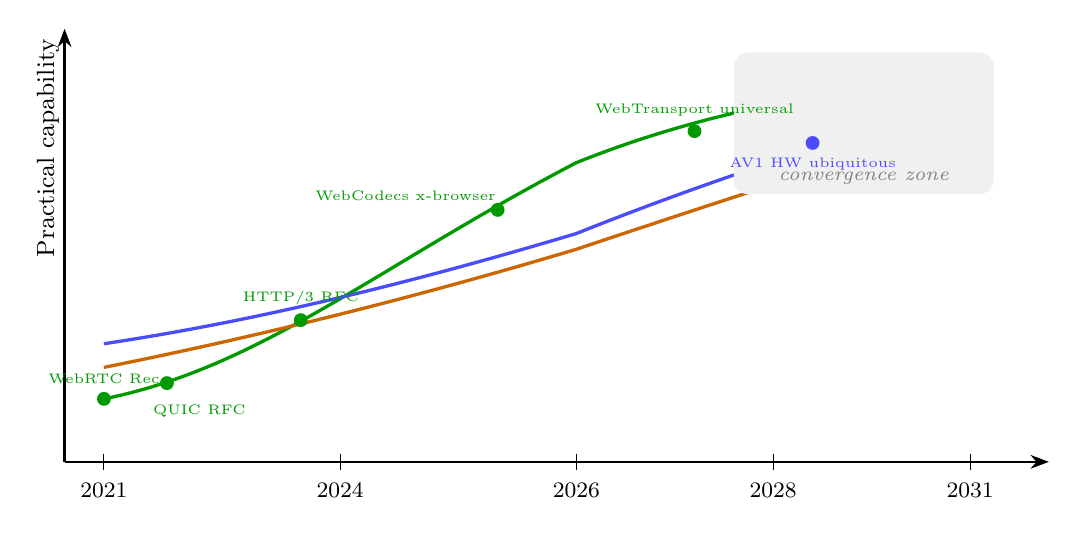
\begin{tikzpicture}[
  >=Stealth,
]

% --- Axes ---
\draw[->, thick] (0, 0) -- (12.5, 0) node[anchor=north, font=\small] {};
\draw[->, thick] (0, 0) -- (0, 5.5) node[anchor=east, font=\small, rotate=90,
  yshift=6pt] {Practical capability};

% Year labels
\foreach \x/\yr in {0.5/2021, 3.5/2024, 6.5/2026, 9/2028, 11.5/2031} {
  \draw (\x, -0.1) -- (\x, 0.1);
  \node[font=\footnotesize, anchor=north] at (\x, -0.15) {\yr};
}

% --- Standards maturity curve (green) ---
\draw[very thick, green!60!black]
  (0.5, 0.8) .. controls (2.5, 1.2) and (4, 2.5) ..
  (6.5, 3.8) .. controls (8, 4.4) and (9.5, 4.7) ..
  (11.5, 4.9);
\node[font=\scriptsize, green!60!black, anchor=south west] at (10.2, 4.85)
  {Standards};

% --- Hardware capability curve (blue) ---
\draw[very thick, blue!70]
  (0.5, 1.5) .. controls (2.5, 1.8) and (4.5, 2.3) ..
  (6.5, 2.9) .. controls (8, 3.5) and (9.5, 4.0) ..
  (11.5, 4.6);
\node[font=\scriptsize, blue!70, anchor=south west] at (10.2, 4.4)
  {Hardware};

% --- Network bandwidth curve (orange) ---
\draw[very thick, orange!80!black]
  (0.5, 1.2) .. controls (2.5, 1.6) and (4.5, 2.1) ..
  (6.5, 2.7) .. controls (8, 3.2) and (9.5, 3.7) ..
  (11.5, 4.3);
\node[font=\scriptsize, orange!80!black, anchor=south west] at (10.2, 3.95)
  {Network};

% --- Convergence zone ---
\fill[gray!12, rounded corners=5pt] (8.5, 3.4) rectangle (11.8, 5.2);
\node[font=\scriptsize\itshape, text=black!50, align=center] at (10.15, 3.6)
  {convergence zone};

% --- Key milestones (annotation dots) ---
% WebRTC 1.0 Rec
\fill[green!60!black] (0.5, 0.8) circle (2.5pt);
\node[font=\tiny, anchor=south, green!60!black, yshift=2pt] at (0.5, 0.8)
  {WebRTC Rec};

% QUIC RFC
\fill[green!60!black] (1.3, 1.0) circle (2.5pt);
\node[font=\tiny, anchor=north west, green!60!black] at (1.0, 0.85)
  {QUIC RFC};

% HTTP/3 RFC
\fill[green!60!black] (3.0, 1.8) circle (2.5pt);
\node[font=\tiny, anchor=south, green!60!black, yshift=2pt] at (3.0, 1.8)
  {HTTP/3 RFC};

% WebCodecs cross-browser
\fill[green!60!black] (5.5, 3.2) circle (2.5pt);
\node[font=\tiny, anchor=south east, green!60!black] at (5.6, 3.2)
  {WebCodecs x-browser};

% WebTransport universal (projected)
\fill[green!60!black] (8.0, 4.2) circle (2.5pt);
\node[font=\tiny, anchor=south, green!60!black, yshift=2pt] at (8.0, 4.2)
  {WebTransport universal};

% AV1 HW ubiquitous
\fill[blue!70] (9.5, 4.05) circle (2.5pt);
\node[font=\tiny, anchor=north, blue!70, yshift=-2pt] at (9.5, 4.05)
  {AV1 HW ubiquitous};

\end{tikzpicture}
\caption{Convergence of standards maturity, hardware capability, and network
  bandwidth from 2021 to 2031. The shaded region marks where all three curves
  reach levels sufficient to fully exploit the standards discussed in this
  document.}
\label{fig:convergence}
\end{figure}

\section{Summary}

\begin{table}[ht]
\centering
\small
\renewcommand{\arraystretch}{1.3}
\begin{tabularx}{\textwidth}{lXXX}
\toprule
\textbf{Standard} & \textbf{Late 2021} & \textbf{March 2026} & \textbf{2028--2031 Projection} \\
\midrule
WebRTC 1.0 &
  W3C Rec (Jan 2021). Chrome/Firefox full support. Safari limited: H.264 only, no simulcast, iOS DataChannel broken. Plan~B still in Chrome. &
  Updated Rec (2024--25). Unified Plan universal. Safari has VP9. iOS reliable. JSEP updated to RFC~9429. Encoded Transforms Chrome-only. &
  Encoded Transforms cross-browser. AV1 default codec (HW-accelerated). SFrame for group E2EE. No ``WebRTC 2.0'' --- incremental extensions. \\
\midrule
QUIC &
  RFC~9000 (May 2021). Chrome/Firefox default. Safari experimental, manual opt-in. &
  Default in all browsers (Safari~16+, 2022). &
  QUIC~v2 (RFC~9369) transparent migration. RTP over QUIC (RoQ) at RFC status. \\
\midrule
HTTP/3 &
  Pre-RFC draft implementations. Chrome/Firefox default. Safari behind flag. &
  RFC~9114 (June 2022). Default in all browsers. 92\%+ coverage. &
  Mature universal transport. Foundation for WebTransport and MoQ. \\
\midrule
WebTransport &
  Experimental only. Chrome disabled (M91--94). Firefox/Safari: none. &
  Chrome~97+, Firefox~114+. Safari: still absent. 82\% coverage. &
  Universal (Safari via Interop~2026). W3C Rec. Enables unbundled architecture and MoQ. \\
\midrule
WebCodecs &
  Chrome~94 only (Sept 2021). Firefox/Safari: none. First Public WD. &
  Chrome, Firefox~130+, Safari~26+. 94\% coverage. Still WD. &
  W3C Rec by 2027. AV1 HW encode ubiquitous. Custom media pipelines on all devices. \\
\midrule
MoQ &
  Did not exist. &
  IETF draft (v15, Oct 2025). No browser API. &
  RFC status. JS libraries on WebTransport + WebCodecs. Sub-second CDN streaming. \\
\bottomrule
\end{tabularx}
\caption{Browser capability status by standard across the full 2021--2031 timeline.}
\label{tab:summary}
\end{table}

\section{Conclusion}

This document has traced the real-time web communication stack across a full
decade, from its fragmented state in late 2021 through its current maturity in
March 2026 to its projected convergence by 2031.

In late 2021, the stack was transitional. WebRTC was the only finalized
standard with broad browser support, yet even it suffered from significant
cross-browser inconsistencies --- Safari's codec and feature limitations,
Chrome's ongoing SDP migration, and iOS reliability issues. QUIC had just been
standardized but was not yet universally enabled. HTTP/3 was shipping based on
draft specifications. WebTransport was effectively non-functional in any
browser. WebCodecs had just shipped in a single browser. MoQ did not yet exist
as a draft.

By March 2026, the picture is fundamentally different. The core protocol stack
--- from QUIC transport through HTTP/3 to WebRTC --- is standardized via
finalized RFCs and implemented by default across all major browsers. WebCodecs
provides cross-browser access to hardware-accelerated codecs at the frame
level. Two gaps remain: Safari's lack of WebTransport support and the
Chrome-only status of Encoded Transforms for end-to-end encryption.

The 2028--2029 projections close these gaps. WebTransport reaches Safari via
Apple's Interop~2026 commitment. Encoded Transforms become cross-browser.
WebCodecs achieves W3C Recommendation status. AV1 becomes a practical WebRTC
codec as hardware encoding expands. MoQ and RTP over QUIC reach RFC status,
establishing new standards-based paths for media transport. Hardware and
network improvements --- 40--50\% CPU gains since 2021, broadband speeds
approaching 150~Mbps --- ensure these standards land on infrastructure that
can fully exploit them.

By 2029--2031, the stack reaches full convergence. The ``unbundled''
architecture --- composing WebTransport, WebCodecs, and WebAssembly as
alternatives to monolithic \texttt{RTCPeerConnection} --- becomes practically
viable for specialized use cases like cloud gaming, scientific visualization,
and broadcast distribution. AV1 hardware encoding is ubiquitous across the
device spectrum. MoQ on WebTransport enables standards-based sub-second
streaming with CDN fan-out. Network bandwidth (200--300~Mbps fixed, 100+~Mbps
mobile) shifts the constraint from capacity to quality: 4K conferencing,
multi-stream layouts, and high-frame-rate screen sharing become routine.

The central observation is that standards maturation, hardware improvement, and
network growth are complementary, not independent. A standard that reaches
browser universality on hardware that cannot run it efficiently, or over
networks that cannot carry its output, delivers theoretical capability rather
than practical impact. The 2029--2031 timeframe is where all three curves
converge: every standard in this document will be finalized and universally
implemented, running on hardware with dedicated codec acceleration, over
networks with bandwidth to spare. This convergence is what distinguishes the
projected end state from a simple extrapolation of today's capabilities ---
and what makes the full real-time web communication stack, from transport to
codec to application, a resolved problem rather than a work in progress.

\newpage
\appendix
\renewcommand{\thesection}{\Alph{section}}
\renewcommand{\thesubsection}{\Alph{section}.\arabic{subsection}}
\renewcommand{\thesubsubsection}{\Alph{section}.\arabic{subsection}.\arabic{subsubsection}}
% appendix-info-theory.tex
% Standalone appendix — include from retrospective.tex via:
%   \appendix
%   % appendix-info-theory.tex
% Standalone appendix — include from retrospective.tex via:
%   \appendix
%   % appendix-info-theory.tex
% Standalone appendix — include from retrospective.tex via:
%   \appendix
%   \input{appendix-info-theory}
%
% Requires in the preamble: amsmath, amssymb, tabularx, booktabs

\section{Information-Theoretic View}
\label{app:info-theory}

This appendix applies information-theoretic measures to the real-time
web communication stack described in this document. We quantify channel
capacity, source coding efficiency, and effective information rates
across three time horizons: today (March~2026), the near term
(2027--2028), and the medium term (2029--2031). The analysis draws on
the standards, codec parameters, and infrastructure projections
developed in the main text.

\subsection{Channel Capacity of the Transport Layer}

The Shannon-Hartley theorem gives the theoretical maximum information
rate for a channel with additive white Gaussian noise:
\begin{equation}
  C = B \log_2\!\left(1 + \frac{S}{N}\right) \quad \text{[bits/s]}
  \label{eq:shannon}
\end{equation}
where $B$ is the channel bandwidth in Hz and $S/N$ is the
signal-to-noise ratio.

While the physical-layer capacity of a broadband link is governed by
(\ref{eq:shannon}), the \emph{effective} capacity available to the
application is reduced by protocol overhead, congestion control, and
transport inefficiencies. We define the effective application-layer
throughput as:
\begin{equation}
  R_{\text{eff}} = C_{\text{link}} \cdot \eta_{\text{transport}}
    \cdot (1 - \rho_{\text{overhead}})
  \label{eq:reff}
\end{equation}
where $C_{\text{link}}$ is the link-layer capacity,
$\eta_{\text{transport}} \in (0,1]$ is the transport efficiency factor
(capturing congestion control, retransmission, and multiplexing
behavior), and $\rho_{\text{overhead}} \in [0,1)$ is the fractional
protocol overhead (headers, encryption, framing).

\subsubsection{Head-of-Line Blocking and Multiplexed Capacity}

Consider $n$ independent streams multiplexed over a single connection.
Under TCP (HTTP/2), a single lost packet blocks all $n$ streams. The
expected throughput per stream under loss rate $p$ is bounded by:
\begin{equation}
  R_{\text{TCP}}^{(i)} \leq \frac{R_{\text{eff}}}{n}
    \cdot (1 - p)^{n-1}
  \label{eq:hol-tcp}
\end{equation}
because a loss in \emph{any} of the $n$ streams stalls all others. Under
QUIC (RFC~9000), streams are independent at the transport layer, so:
\begin{equation}
  R_{\text{QUIC}}^{(i)} \leq \frac{R_{\text{eff}}}{n}
    \cdot (1 - p)
  \label{eq:hol-quic}
\end{equation}
The ratio of effective per-stream throughput is:
\begin{equation}
  \frac{R_{\text{QUIC}}^{(i)}}{R_{\text{TCP}}^{(i)}}
    = \frac{1}{(1-p)^{n-2}}
  \label{eq:hol-ratio}
\end{equation}
\excursus{Excursus: Why $n = 8$?}{In a typical multi-participant video
conference, each peer contributes multiple concurrent streams: a camera video
track, an audio track, and often a screen-share or data channel. A four-person
call with two media tracks each produces $n = 8$ multiplexed streams over a
single connection --- the reference value used throughout this section. Larger
meetings (e.g.\ 10 participants with simulcast layers) push $n$ higher,
amplifying the HOL blocking effect further.}

For $n = 8$ streams (a typical multi-track video conference) at
$p = 0.01$ (1\% loss), this gives a QUIC advantage factor of
$1/(0.99)^6 \approx 1.062$, a modest 6.2\% improvement. At $p = 0.05$
(5\% loss, common on mobile or congested links), the factor is
$1/(0.95)^6 \approx 1.34$, a 34\% throughput advantage per stream.

\begin{figure}[ht]
\centering
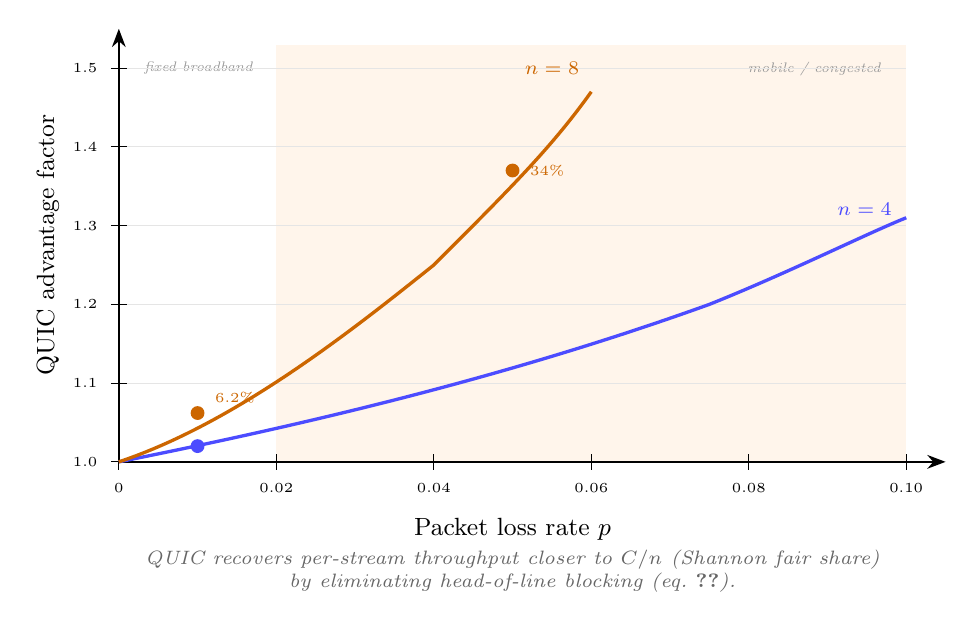
\begin{tikzpicture}[>=Stealth]

% --- Shaded region (drawn FIRST so curves appear on top) ---
\fill[orange!8] (2, 0) rectangle (10, 5.3);
\node[font=\tiny\itshape, text=black!40, anchor=north east] at (9.8, 5.2)
  {mobile / congested};
\node[font=\tiny\itshape, text=black!40, anchor=north west] at (0.2, 5.2)
  {fixed broadband};

% --- Grid lines ---
\foreach \y in {1, 2, 3, 4, 5} {
  \draw[gray!20] (0, \y) -- (10, \y);
}

% --- Axes ---
\draw[->, thick] (0, 0) -- (10.5, 0);
\draw[->, thick] (0, 0) -- (0, 5.5);

% --- Axis titles (positioned to clear tick labels) ---
\node[font=\small] at (5, -0.85) {Packet loss rate $p$};
\node[font=\small, rotate=90] at (-0.9, 2.75) {QUIC advantage factor};

% --- X-axis labels ---
\foreach \x/\lab in {0/0, 2/0.02, 4/0.04, 6/0.06, 8/0.08, 10/0.10} {
  \draw (\x, -0.1) -- (\x, 0.1);
  \node[font=\tiny, anchor=north] at (\x, -0.15) {\lab};
}

% --- Y-axis labels ---
\foreach \y/\lab in {0/1.0, 1/1.1, 2/1.2, 3/1.3, 4/1.4, 5/1.5} {
  \draw (-0.1, \y) -- (0.1, \y);
  \node[font=\tiny, anchor=east] at (-0.15, \y) {\lab};
}

% --- n=4 curve: 1/(1-p)^2 ---
\draw[very thick, blue!70]
  (0, 0) .. controls (2.5, 0.5) and (5, 1.1) ..
  (7.5, 2.0) .. controls (8.5, 2.4) and (9.5, 2.9) ..
  (10, 3.1);
\node[font=\scriptsize, blue!70, anchor=south west] at (9.0, 3.0)
  {$n = 4$};

% --- n=8 curve: 1/(1-p)^6 ---
\draw[very thick, orange!80!black]
  (0, 0) .. controls (1.5, 0.5) and (3, 1.7) ..
  (4, 2.5) .. controls (5, 3.5) and (5.5, 4.0) ..
  (6, 4.7);
\node[font=\scriptsize, orange!80!black, anchor=south] at (5.5, 4.8)
  {$n = 8$};

% --- Reference points ---
\fill[orange!80!black] (1.0, 0.62) circle (2.5pt);
\node[font=\tiny, orange!80!black, anchor=south west] at (1.1, 0.62)
  {6.2\%};

\fill[orange!80!black] (5.0, 3.7) circle (2.5pt);
\node[font=\tiny, orange!80!black, anchor=west] at (5.1, 3.7)
  {34\%};

\fill[blue!70] (1.0, 0.20) circle (2.5pt);

% --- Annotation ---
\node[font=\scriptsize\itshape, text=black!60, align=center,
  anchor=north] at (5.0, -1.0)
  {QUIC recovers per-stream throughput closer to $C/n$ (Shannon fair share)\\
   by eliminating head-of-line blocking (eq.~\ref{eq:hol-ratio}).};

\end{tikzpicture}
\caption{QUIC advantage factor $1/(1-p)^{n-2}$ over TCP for multiplexed
  streams. At 5\% loss with $n=8$ streams, QUIC delivers 34\% more
  per-stream throughput by maintaining independence at the transport layer.}
\label{fig:hol-blocking}
\end{figure}

\subsubsection{Connection Establishment Latency}

Let $\tau$ denote the one-way latency (half the round-trip time). The
information-carrying capacity during connection establishment is zero;
the handshake represents pure overhead. The time to first useful byte
is:
\begin{align}
  T_{\text{TCP+TLS\,1.3}} &= 2\tau_{\text{TCP}} + \tau_{\text{TLS}}
    = 3\tau \quad \text{(1-RTT TLS~1.3)} \label{eq:tcp-setup} \\
  T_{\text{QUIC}} &= \tau \quad \text{(1-RTT)}
    \label{eq:quic-setup} \\
  T_{\text{QUIC,\,0-RTT}} &= 0 \quad \text{(resumption)}
    \label{eq:quic-0rtt}
\end{align}
The QUIC 0-RTT case (\ref{eq:quic-0rtt}) eliminates the handshake
entirely for resumed connections. The information lost during
handshake dead time, relative to steady-state capacity, is:
\begin{equation}
  I_{\text{lost}} = C_{\text{link}} \cdot T_{\text{setup}}
  \label{eq:ilost}
\end{equation}
For a 120~Mbps link with $\tau = 25$~ms (typical fixed broadband in
2026), the TCP+TLS~1.3 handshake wastes $120 \times 10^6 \times 0.075
= 9 \times 10^6$ bits (1.125~MB), while QUIC~1-RTT wastes only
$3 \times 10^6$ bits (375~KB).

\subsection{Source Coding Efficiency}

The rate-distortion function $R(D)$ defines the minimum bit rate
required to represent a source at distortion level $D$. For a
Gaussian source with variance $\sigma^2$ under mean squared error
distortion:
\begin{equation}
  R(D) = \frac{1}{2} \log_2 \frac{\sigma^2}{D}
    \quad \text{[bits/sample]}
  \label{eq:rate-distortion}
\end{equation}

\excursus{Excursus: Why Gaussian source?}{The Gaussian memoryless model is used
because it yields the highest (worst-case) $R(D)$ among all sources of equal
variance. Any codec that approaches the Gaussian bound on real video is
therefore doing at least as well as the bound predicts --- the true $R(D)$ for
spatially and temporally correlated video lies below the Gaussian curve, making
it a conservative benchmark.}

No practical codec achieves $R(D)$;\footnote{The $R(D)$ curve in
Figure~\ref{fig:rate-distortion} is the Gaussian memoryless source bound
(equation~\ref{eq:rate-distortion}), which is an upper bound on the true
$R(D)$ for non-Gaussian sources such as video.  Additionally, $R(D)$ assumes
zero excess-distortion probability, whereas practical codecs permit a
frame-level excess-distortion probability on the order of $10^{-6}$ to
$10^{-8}$.  Both factors allow codec operating points measured on real content
to approach or marginally cross the Gaussian bound.} real codecs operate at
some rate $R_{\text{codec}} > R(D)$. We define the coding efficiency gap as:
\begin{equation}
  \Delta = \frac{R_{\text{codec}} - R(D)}{R(D)}
  \label{eq:coding-gap}
\end{equation}

The codecs in the WebRTC stack can be ordered by their empirical
proximity to $R(D)$ for typical video content at conversational
resolutions (720p, 30~fps). Using published Bj\o ntegaard Delta (BD)
rate measurements:
\begin{equation}
  R_{\text{H.264}} > R_{\text{VP9}} > R_{\text{AV1}}
    > R(D)
  \label{eq:codec-ordering}
\end{equation}

Specifically, the empirical rate savings at equivalent PSNR are
approximately:
\begin{align}
  R_{\text{VP9}}  &\approx 0.65 \cdot R_{\text{H.264}}
    \quad (\sim\!35\% \text{ savings}) \label{eq:vp9-savings} \\
  R_{\text{AV1}}  &\approx 0.70 \cdot R_{\text{VP9}}
    \approx 0.46 \cdot R_{\text{H.264}}
    \quad (\sim\!30\% \text{ over VP9})
  \label{eq:av1-savings}
\end{align}

\begin{figure}[ht]
\centering
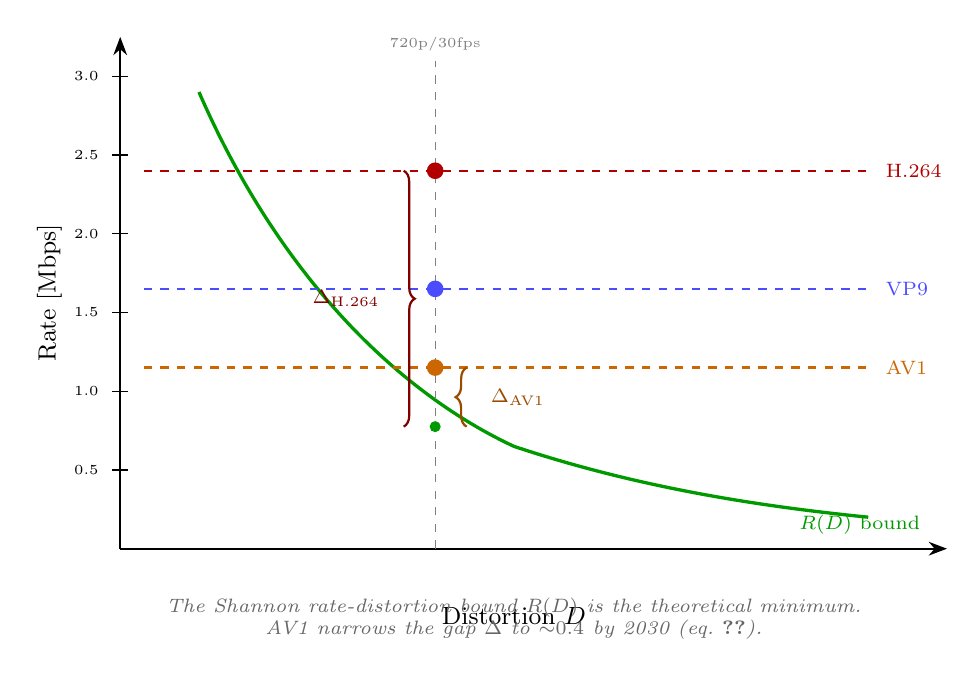
\begin{tikzpicture}[>=Stealth]

% --- Axes ---
\draw[->, thick] (0, 0) -- (10.5, 0);
\draw[->, thick] (0, 0) -- (0, 6.5);

% --- Axis titles ---
\node[font=\small] at (5, -0.85) {Distortion $D$};
\node[font=\small, rotate=90] at (-0.9, 3.25) {Rate [Mbps]};

% --- Y-axis rate labels ---
\foreach \y/\lab in {1.0/0.5, 2.0/1.0, 3.0/1.5, 4.0/2.0, 5.0/2.5, 6.0/3.0} {
  \draw (-0.1, \y) -- (0.1, \y);
  \node[font=\tiny, anchor=east] at (-0.15, \y) {\lab};
}

% --- R(D) Shannon bound curve ---
\draw[very thick, green!60!black]
  (1.0, 5.8) .. controls (2.0, 3.5) and (3.5, 2.0) ..
  (5.0, 1.3) .. controls (6.5, 0.8) and (8.0, 0.55) ..
  (9.5, 0.4);
\node[font=\scriptsize, green!60!black, anchor=north west] at (8.5, 0.55)
  {$R(D)$ bound};

% --- Reference distortion line (720p/30fps operating point) ---
\draw[thin, gray, dashed] (4.0, 0) -- (4.0, 6.2);
\node[font=\tiny, gray, anchor=south] at (4.0, 6.2) {720p/30fps};

% --- R(D) value at reference distortion ---
\fill[green!60!black] (4.0, 1.55) circle (2pt);

% --- Codec operating points at reference distortion ---
% H.264: ~2.5 Mbps
\draw[thick, dashed, red!70!black] (0.3, 4.8) -- (9.5, 4.8);
\fill[red!70!black] (4.0, 4.8) circle (3pt);
\node[font=\scriptsize, red!70!black, anchor=west] at (9.6, 4.8) {H.264};

% VP9: ~1.6 Mbps (0.65 * H.264)
\draw[thick, dashed, blue!70] (0.3, 3.3) -- (9.5, 3.3);
\fill[blue!70] (4.0, 3.3) circle (3pt);
\node[font=\scriptsize, blue!70, anchor=west] at (9.6, 3.3) {VP9};

% AV1: ~1.15 Mbps (0.46 * H.264)
\draw[thick, dashed, orange!80!black] (0.3, 2.3) -- (9.5, 2.3);
\fill[orange!80!black] (4.0, 2.3) circle (3pt);
\node[font=\scriptsize, orange!80!black, anchor=west] at (9.6, 2.3) {AV1};

% --- Gap annotations (braces) ---
% H.264 gap
\draw[decorate, decoration={brace, amplitude=4pt, mirror},
  thick, red!50!black]
  (3.6, 1.55) -- (3.6, 4.8)
  node[midway, anchor=east, font=\scriptsize, xshift=-5pt]
  {$\Delta_{\text{H.264}}$};

% AV1 gap
\draw[decorate, decoration={brace, amplitude=4pt},
  thick, orange!60!black]
  (4.4, 1.55) -- (4.4, 2.3)
  node[midway, anchor=west, font=\scriptsize, xshift=5pt]
  {$\Delta_{\text{AV1}}$};

% --- Annotation ---
\node[font=\scriptsize\itshape, text=black!60, align=center,
  anchor=north] at (5.0, -0.5)
  {The Shannon rate-distortion bound $R(D)$ is the theoretical minimum.\\
   AV1 narrows the gap $\Delta$ to ${\sim}0.4$ by 2030 (eq.~\ref{eq:coding-gap}).};

\end{tikzpicture}
\caption{Codec operating rates vs.\ the Shannon rate-distortion bound $R(D)$
  at 720p/30fps. Each codec operates above the theoretical minimum; the gap
  $\Delta$ (eq.~\ref{eq:coding-gap}) shrinks from H.264 through VP9 to AV1,
  approaching but never reaching the bound.}
\label{fig:rate-distortion}
\end{figure}

\subsubsection{Codec Entropy and WebCodecs}

The WebCodecs API (W3C Working Draft) exposes per-frame codec access,
allowing measurement and control of the instantaneous encoding rate.
For a video frame $f_t$ at time $t$, the encoder output has empirical
entropy:
\begin{equation}
  \hat{H}(f_t) = -\sum_{s \in \mathcal{S}}
    p(s \mid f_t) \log_2 p(s \mid f_t)
  \label{eq:frame-entropy}
\end{equation}
where $\mathcal{S}$ is the set of symbols emitted by the entropy coder
(CABAC for H.264/AV1, arithmetic coding for VP9). WebCodecs enables
applications to observe $|E(f_t)|$ (the encoded frame size in bits)
directly, which serves as a practical upper bound on
$\hat{H}(f_t)$:
\begin{equation}
  \hat{H}(f_t) \leq |E(f_t)| \leq R_{\text{codec}} / \text{fps}
  \label{eq:entropy-bound}
\end{equation}

\subsection{Effective Information Rate by Time Horizon}

We now combine transport and source coding measures to estimate the
effective information rate for a representative real-time video
session: a single 720p/30fps video call with one audio channel.

\excursus{Excursus: Why 720p?}{Throughout this appendix, 720p/30fps is used as
a fixed reference for cross-era comparison, not as a prediction that 720p
remains the dominant conferencing resolution. The bandwidth surplus quantified
below is precisely what enables migration to 1080p (feasible by ${\sim}$2028
with AV1 hardware encode at today's 720p bit rates) and 4K (feasible by
${\sim}$2030). The 720p baseline makes the efficiency gains legible: the same
task gets cheaper, freeing capacity for higher quality or more streams.}

Define the \emph{net information rate} as:
\begin{equation}
  I_{\text{net}} = R_{\text{codec}} \cdot \eta_{\text{transport}}
    \cdot (1 - \rho_{\text{overhead}})
    \cdot (1 - p_{\text{loss}})
  \label{eq:inet}
\end{equation}

\begin{table}[ht]
\centering
\small
\renewcommand{\arraystretch}{1.4}
\begin{tabularx}{\textwidth}{lXXX}
\toprule
\textbf{Parameter} & \textbf{March 2026} & \textbf{2027--2028} &
  \textbf{2029--2031} \\
\midrule
Median link capacity &
  120~Mbps &
  $\sim$150~Mbps &
  200--300~Mbps \\
Dominant codec (WebRTC) &
  VP9 / H.264 &
  VP9 / AV1 (HW) &
  AV1 (HW default) \\
Codec rate (720p/30fps) &
  1.5--2.5~Mbps &
  1.0--1.8~Mbps &
  0.7--1.2~Mbps \\
$\eta_{\text{transport}}$ &
  0.92 (QUIC) &
  0.93 &
  0.94 \\
$\rho_{\text{overhead}}$ (SRTP+QUIC) &
  0.06 &
  0.05 &
  0.04 \\
Typical loss $p$ &
  0.01--0.03 &
  0.01--0.02 &
  0.005--0.01 \\
$I_{\text{net}}$ (720p video) &
  1.3--2.2~Mbps &
  0.9--1.6~Mbps &
  0.6--1.1~Mbps \\
$I_{\text{net}}$ as \% of $C_{\text{link}}$ &
  1.1--1.8\% &
  0.6--1.1\% &
  0.2--0.6\% \\
\bottomrule
\end{tabularx}
\caption{Effective information rate for a 720p/30fps WebRTC video stream.
  The declining ratio $I_{\text{net}} / C_{\text{link}}$ reflects both
  improved codec efficiency and growing link capacity, freeing bandwidth
  for higher resolutions, additional streams, or concurrent data
  channels.}
\label{tab:inet}
\end{table}

The declining ratio $I_{\text{net}} / C_{\text{link}}$ in
Table~\ref{tab:inet} is the central quantitative observation: by 2030, a
720p video call consumes less than 0.5\% of available link capacity. The
surplus capacity enables qualitative changes --- 4K video conferencing,
multi-stream layouts, or concurrent data channels via WebTransport ---
that are quantitatively infeasible in 2026.

\begin{figure}[ht]
\centering
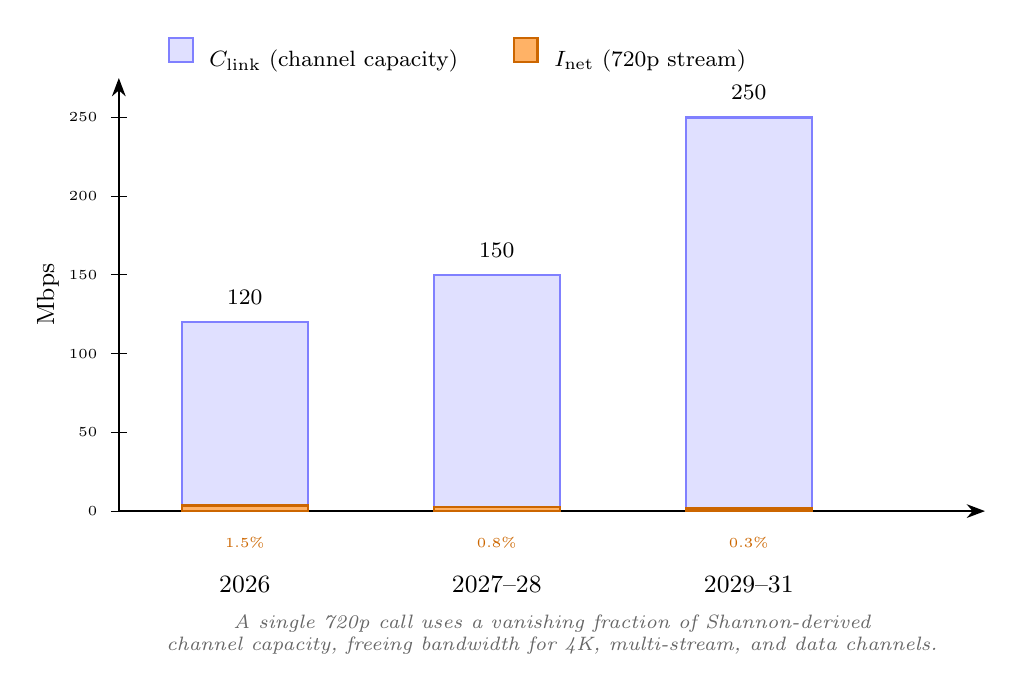
\begin{tikzpicture}[>=Stealth]

% --- Axes ---
\draw[->, thick] (0, 0) -- (11, 0);
\draw[->, thick] (0, 0) -- (0, 5.5);

% --- Axis title ---
\node[font=\small, rotate=90] at (-0.9, 2.75) {Mbps};

% --- Y-axis labels ---
\foreach \y/\lab in {0/0, 1/50, 2/100, 3/150, 4/200, 5/250} {
  \draw (-0.1, \y) -- (0.1, \y);
  \node[font=\tiny, anchor=east] at (-0.15, \y) {\lab};
}

% --- Group: March 2026 ---
% C_link = 120 Mbps -> y = 2.4
\fill[blue!12] (0.8, 0) rectangle (2.4, 2.4);
\draw[blue!50, thick] (0.8, 0) rectangle (2.4, 2.4);
% I_net = 1.75 Mbps (midpoint) -> y = 0.035
\fill[orange!60] (0.8, 0) rectangle (2.4, 0.07);
\draw[orange!80!black, thick] (0.8, 0) rectangle (2.4, 0.07);
\node[font=\footnotesize, anchor=south] at (1.6, 2.5) {120};
\node[font=\tiny, orange!80!black] at (1.6, -0.4) {1.5\%};
\node[font=\small, anchor=north] at (1.6, -0.7) {2026};

% --- Group: 2027--2028 ---
% C_link = 150 Mbps -> y = 3.0
\fill[blue!12] (4.0, 0) rectangle (5.6, 3.0);
\draw[blue!50, thick] (4.0, 0) rectangle (5.6, 3.0);
% I_net = 1.25 Mbps (midpoint) -> y = 0.025
\fill[orange!60] (4.0, 0) rectangle (5.6, 0.05);
\draw[orange!80!black, thick] (4.0, 0) rectangle (5.6, 0.05);
\node[font=\footnotesize, anchor=south] at (4.8, 3.1) {150};
\node[font=\tiny, orange!80!black] at (4.8, -0.4) {0.8\%};
\node[font=\small, anchor=north] at (4.8, -0.7) {2027--28};

% --- Group: 2029--2031 ---
% C_link = 250 Mbps -> y = 5.0
\fill[blue!12] (7.2, 0) rectangle (8.8, 5.0);
\draw[blue!50, thick] (7.2, 0) rectangle (8.8, 5.0);
% I_net = 0.85 Mbps (midpoint) -> y = 0.017
\fill[orange!60] (7.2, 0) rectangle (8.8, 0.034);
\draw[orange!80!black, thick] (7.2, 0) rectangle (8.8, 0.034);
\node[font=\footnotesize, anchor=south] at (8.0, 5.1) {250};
\node[font=\tiny, orange!80!black] at (8.0, -0.4) {0.3\%};
\node[font=\small, anchor=north] at (8.0, -0.7) {2029--31};

% --- Legend ---
\node[anchor=west, font=\footnotesize] at (0.5, 5.8) {%
  \tikz[baseline=-0.5ex]{\fill[blue!12] (0,0) rectangle (0.3,0.3);
    \draw[blue!50, thick] (0,0) rectangle (0.3,0.3);}
  ~$C_{\text{link}}$ (channel capacity) \qquad
  \tikz[baseline=-0.5ex]{\fill[orange!60] (0,0) rectangle (0.3,0.3);
    \draw[orange!80!black, thick] (0,0) rectangle (0.3,0.3);}
  ~$I_{\text{net}}$ (720p stream)};

% --- Annotation ---
\node[font=\scriptsize\itshape, text=black!60, align=center,
  anchor=north] at (5.5, -1.2)
  {A single 720p call uses a vanishing fraction of Shannon-derived\\
   channel capacity, freeing bandwidth for 4K, multi-stream, and data channels.};

\end{tikzpicture}
\caption{Channel capacity $C_{\text{link}}$ vs.\ effective information rate
  $I_{\text{net}}$ for a single 720p/30fps stream across time horizons. The
  orange bar (stream rate) is barely visible against the blue bar (capacity),
  illustrating the growing surplus as codecs improve and bandwidth increases.}
\label{fig:inet-capacity}
\end{figure}

\subsection{Security Entropy and Key Space}

The DTLS-SRTP security architecture (RFCs~8827, 3711) protects all
WebRTC media. Information-theoretic security requires that the key
entropy exceed the information content of the protected material.

For a DTLS~1.3 handshake with ECDHE on P-256, the key agreement
provides:
\begin{equation}
  H_{\text{key}} = 128 \text{~bits of security}
  \label{eq:key-entropy}
\end{equation}

The SRTP master key is 128 bits (AES-128-GCM), giving an exhaustive
search cost of $2^{128}$ operations. The total information content of a
one-hour 720p video call at 2~Mbps is:
\begin{equation}
  I_{\text{call}} = 2 \times 10^6 \times 3600
    = 7.2 \times 10^9 \text{~bits}
    \approx 2^{32.7} \text{~bits}
  \label{eq:call-content}
\end{equation}

The ratio of key entropy to protected content:
\begin{equation}
  \frac{H_{\text{key}}}{I_{\text{call}}}
    = \frac{128}{32.7} \approx 3.91
  \label{eq:security-margin}
\end{equation}

This ratio remains comfortably above~1 even for much longer sessions.
For a continuous 24-hour 4K AV1 stream at 15~Mbps:
\begin{equation}
  I_{\text{stream}} = 15 \times 10^6 \times 86400
    = 1.296 \times 10^{12} \text{~bits}
    \approx 2^{40.2} \text{~bits}
\end{equation}
yielding $H_{\text{key}} / I_{\text{stream}} \approx 3.18$, still
well above the threshold.

\subsubsection{End-to-End Encryption via Encoded Transforms}

The RTCRtpScriptTransform API (Encoded Transforms) enables
application-layer E2EE within the WebRTC pipeline. From an
information-theoretic perspective, this introduces a second encryption
layer with its own key, creating a \emph{nested channel}:
\begin{equation}
  X \xrightarrow{\;K_{\text{E2EE}}\;}
  E_1(X) \xrightarrow{\;K_{\text{SRTP}}\;}
  E_2(E_1(X))
  \label{eq:nested}
\end{equation}

The mutual information between the ciphertext and plaintext, given
neither key, satisfies:
\begin{equation}
  I\!\left(X;\, E_2(E_1(X))\right) \leq
    \min\!\big(H(K_{\text{E2EE}})^{-1},\;
    H(K_{\text{SRTP}})^{-1}\big)
    \cdot I_{\text{call}}
  \label{eq:mutual-e2ee}
\end{equation}

In practice, with $H(K_{\text{E2EE}}) = H(K_{\text{SRTP}}) = 128$
bits, this quantity is negligible ($\ll 1$ bit for any practical
session length), confirming that the nested encryption provides
information-theoretic confidentiality well beyond computational
security guarantees.

Today (March~2026), Encoded Transforms remain Chrome-only. By
2027--2028 (Section~8.3), cross-browser standardization will make
this nested channel universally available. By 2029--2031, SFrame
for group calls will extend this to $n$-party sessions, where the
mutual information between any non-member and the group plaintext
remains negligible:
\begin{equation}
  I\!\left(X;\, E(X) \;\middle|\; K_i \notin
    \{K_1, \ldots, K_n\}\right) \approx 0
  \label{eq:sframe}
\end{equation}

\subsection{WebTransport: Unreliable Datagrams and Channel Capacity}

WebTransport (RFC~9297) introduces unreliable datagrams to browser-server
communication. For latency-sensitive applications (game state, sensor
telemetry), the relevant measure is not throughput but
\emph{freshness-weighted information rate}. Define the value of a
datagram as exponentially decaying with delivery latency $\delta$:
\begin{equation}
  V(\delta) = e^{-\lambda \delta}
  \label{eq:freshness}
\end{equation}
where $\lambda > 0$ is an application-specific decay rate. The
effective information rate under unreliable delivery is:
\begin{equation}
  I_{\text{WT}} = R_{\text{send}} \cdot (1 - p_{\text{loss}})
    \cdot \mathbb{E}\!\left[e^{-\lambda \delta}\right]
  \label{eq:iwt}
\end{equation}

Under reliable delivery (TCP/WebSocket), a retransmission delays
subsequent data, so:
\begin{equation}
  I_{\text{WS}} = R_{\text{send}}
    \cdot \mathbb{E}\!\left[e^{-\lambda(\delta + p \cdot 2\tau)}\right]
  \label{eq:iws}
\end{equation}

The ratio $I_{\text{WT}} / I_{\text{WS}}$ exceeds 1 when:
\begin{equation}
  (1 - p) \cdot e^{\lambda \cdot p \cdot 2\tau} > 1
  \quad \Longleftrightarrow \quad
  \lambda > \frac{-\ln(1 - p)}{2 p \tau}
  \label{eq:wt-advantage}
\end{equation}

For $p = 0.02$ and $\tau = 25$~ms, this gives $\lambda > 20.2$~s$^{-1}$
(half-life $< 34$~ms).

\excursus{Excursus: Why $p = 0.02$ and $\tau = 25$\,ms?}{These values represent
median fixed-broadband conditions in 2026 (Table~\ref{tab:inet}). On mobile or
congested links ($p \approx 0.05$, $\tau \approx 50$\,ms), the threshold
$\lambda^*$ drops to ${\sim}10$\,s$^{-1}$, broadening WebTransport's advantage
to applications with data half-lives up to ${\sim}70$\,ms. The fixed-broadband
reference is thus conservative: mobile scenarios favor unreliable delivery even
more strongly.}

Any application where data older than
$\sim$30~ms is useless benefits from WebTransport's unreliable
mode over WebSocket --- precisely the regime of interactive gaming, live
cursor tracking, and real-time sensor feeds.

As of March~2026, Safari does not support WebTransport
(Section~5), limiting coverage to $\sim$82\%. By 2027--2028
(Section~8.2), universal support will allow applications to rely on
(\ref{eq:iwt}) without fallback paths.

\begin{figure}[ht]
\centering
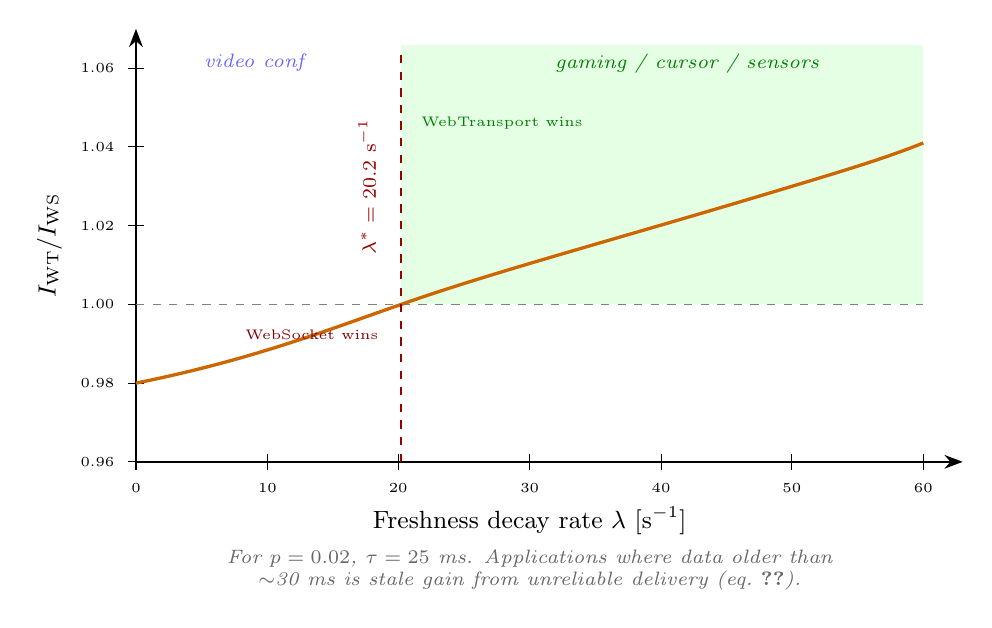
\begin{tikzpicture}[>=Stealth]

% --- Axes ---
\draw[->, thick] (0, 0) -- (10.5, 0);
\draw[->, thick] (0, 0) -- (0, 5.5);

% --- Axis titles (positioned to clear tick labels) ---
\node[font=\small] at (5, -0.75)
  {Freshness decay rate $\lambda$ [s$^{-1}$]};
\node[font=\small, rotate=90] at (-1.1, 2.75)
  {$I_{\text{WT}} / I_{\text{WS}}$};

% --- X-axis labels ---
\foreach \x/\lab in {0/0, 1.67/10, 3.33/20, 5.0/30, 6.67/40, 8.33/50, 10/60} {
  \draw (\x, -0.1) -- (\x, 0.1);
  \node[font=\tiny, anchor=north] at (\x, -0.15) {\lab};
}

% --- Y-axis labels (0.96 to 1.06, each 0.02 = 1 unit) ---
\foreach \y/\lab in {0/0.96, 1/0.98, 2/1.00, 3/1.02, 4/1.04, 5/1.06} {
  \draw (-0.1, \y) -- (0.1, \y);
  \node[font=\tiny, anchor=east] at (-0.15, \y) {\lab};
}

% --- Ratio = 1.0 line (y=2 maps to ratio 1.0) ---
\draw[thin, gray, dashed] (0, 2) -- (10, 2);

% --- Shade WebTransport advantage region ---
% lambda* = 20.2 -> x = 3.37
\fill[green!10] (3.37, 2) rectangle (10, 5.3);

% --- I_WT/I_WS curve: 0.98*exp(lambda*0.001) ---
% Y range: 0.96-1.06 (each 0.02 = 1 unit). lambda=0: y=1, lambda*=20.2: y=2, lambda=60: y=4.05
\draw[very thick, orange!80!black]
  (0, 1.0) .. controls (1.5, 1.3) and (2.5, 1.7) ..
  (3.37, 2.0) .. controls (4.5, 2.4) and (6, 2.8) ..
  (8, 3.4) .. controls (9, 3.7) and (9.5, 3.85) ..
  (10, 4.05);

% --- Threshold line ---
\draw[thick, dashed, red!60!black] (3.37, 0) -- (3.37, 5.2);
\node[font=\scriptsize, red!60!black, anchor=south, rotate=90] at (3.17, 3.5)
  {$\lambda^* = 20.2$ s$^{-1}$};

% --- Application regime labels ---
\node[font=\scriptsize\itshape, text=blue!60, anchor=north] at (1.5, 5.3)
  {video conf};
\node[font=\scriptsize\itshape, text=green!50!black, anchor=north] at (7.0, 5.3)
  {gaming / cursor / sensors};

% --- Mark advantage/disadvantage ---
\node[font=\tiny, text=red!50!black, anchor=north east] at (3.2, 1.8)
  {WebSocket wins};
\node[font=\tiny, text=green!50!black, anchor=north west] at (3.5, 4.5)
  {WebTransport wins};

% --- Annotation ---
\node[font=\scriptsize\itshape, text=black!60, align=center,
  anchor=north] at (5.0, -1.0)
  {For $p = 0.02$, $\tau = 25$~ms. Applications where data older than\\
   ${\sim}$30~ms is stale gain from unreliable delivery (eq.~\ref{eq:wt-advantage}).};

\end{tikzpicture}
\caption{Freshness-weighted information rate ratio $I_{\text{WT}} / I_{\text{WS}}$
  as a function of decay rate $\lambda$. Above the threshold $\lambda^*$,
  WebTransport's unreliable datagrams deliver more useful information per
  unit time than WebSocket's reliable delivery, because retransmission
  wastes capacity on stale data.}
\label{fig:freshness}
\end{figure}

\subsection{Projections Summary and Practical Implications}

\begin{table}[ht]
\centering
\small
\renewcommand{\arraystretch}{1.4}
\begin{tabularx}{\textwidth}{lXXX}
\toprule
\textbf{Measure} & \textbf{March 2026} & \textbf{2027--2028} &
  \textbf{2029--2031} \\
\midrule
Channel capacity $C_{\text{link}}$ &
  120~Mbps &
  150~Mbps &
  250~Mbps \\
HOL blocking factor $(1\!-\!p)^{n-2}$ at $n\!=\!8$ &
  0.94 ($p\!=\!0.01$) &
  0.94 &
  0.97 ($p\!=\!0.005$) \\
Source coding gap $\Delta$ &
  VP9: $\sim$0.8 &
  AV1 HW: $\sim$0.5 &
  AV1 opt: $\sim$0.4 \\
$I_{\text{net}}$ per 720p stream &
  1.3--2.2~Mbps &
  0.9--1.6~Mbps &
  0.6--1.1~Mbps \\
Max 720p streams in $C_{\text{link}}$ &
  $\sim$55--90 &
  $\sim$95--165 &
  $\sim$230--415 \\
E2EE availability &
  Chrome only &
  Cross-browser &
  SFrame $n$-party \\
WebTransport coverage &
  82\% &
  $\sim$100\% &
  100\% \\
Freshness threshold $\lambda^*$ &
  20.2~s$^{-1}$ &
  $\sim$18~s$^{-1}$ &
  $\sim$15~s$^{-1}$ \\
\bottomrule
\end{tabularx}
\caption{Information-theoretic measures across time horizons. $\Delta$
  is the coding efficiency gap (\ref{eq:coding-gap}), $I_{\text{net}}$
  is the net information rate (\ref{eq:inet}), and $\lambda^*$ is the
  freshness decay threshold above which WebTransport dominates WebSocket
  (\ref{eq:wt-advantage}).}
\label{tab:projections}
\end{table}

The trajectory is clear: the combination of improving source coding
(AV1 hardware), expanding channel capacity (broadband growth), and
maturing transport protocols (QUIC universal, WebTransport universal)
drives the \emph{information cost per unit of communicated experience}
steadily downward. The remaining question is not whether the
Shannon capacity suffices --- it already does, by orders of magnitude
--- but how efficiently the protocol stack converts that capacity into
delivered, fresh, secure information at the application layer. By
2030, the gap between theoretical capacity and realized throughput will
be the narrowest it has ever been for browser-based real-time
communication.

\subsubsection{What the Theory Means for Applications}

The equations and figures in this appendix are not purely academic. Each
theoretical result maps to a concrete design decision that application
developers face today and over the next five years.

\textbf{Codec selection determines bandwidth cost, not quality.}
The rate-distortion analysis (Section~A.2, Figure~\ref{fig:rate-distortion})
shows that AV1 operates at roughly 46\% of H.264's bit rate for equivalent
perceptual quality at 720p. In practice, this means a WebRTC application
switching from H.264 to AV1 can either halve its bandwidth consumption at
the same quality or substantially increase resolution (e.g., 720p to 1080p)
within the same bandwidth envelope. By 2030, with AV1 hardware encoding
ubiquitous and the coding gap $\Delta$ approaching 0.4, further codec
improvements yield diminishing returns --- the stack will be operating close
enough to the Shannon rate-distortion bound that the next generation of
efficiency gains will come from transport and architecture, not codecs alone.

\textbf{QUIC's advantage is situational but decisive on bad networks.}
The head-of-line blocking analysis (Section~A.1.1,
Figure~\ref{fig:hol-blocking}) shows that QUIC's per-stream throughput
advantage over TCP is modest on good networks (6\% at 1\% loss) but
substantial on degraded ones (34\% at 5\% loss). The practical implication
is that applications targeting mobile users, emerging markets, or congested
enterprise networks --- precisely the environments where real-time
communication is hardest --- benefit disproportionately from QUIC-based
transports. For a video conference with 8 participants on a cellular
connection experiencing 3--5\% packet loss, the difference between QUIC and
TCP is the difference between usable and degraded video.

\textbf{Connection latency is a solved problem for returning users.}
The handshake analysis (Section~A.1.2) shows that QUIC 0-RTT eliminates
connection establishment overhead entirely for resumed connections. For a
WebTransport application that a user opens daily --- a collaboration tool,
a live dashboard, a recurring meeting client --- the time to first useful
byte drops to zero. The 1.125~MB of wasted capacity during a TCP+TLS
handshake on a 120~Mbps link may seem small, but for latency-sensitive
applications where the first 100~ms of perceived responsiveness determines
user experience, the difference is measurable.

\textbf{Bandwidth surplus enables architectural ambition.}
The effective information rate analysis (Section~A.3,
Figure~\ref{fig:inet-capacity}) reveals the most consequential practical
finding: a single 720p video stream consumes a vanishing fraction of
available link capacity (under 0.5\% by 2030). This surplus is not merely
``headroom'' --- it is the resource that makes new application architectures
feasible. A 250~Mbps link can theoretically carry 230--415 simultaneous 720p
streams. In practice, this means applications can afford to run multiple
concurrent media flows (video, screen share, spatial audio), data channels
(collaborative editing, file transfer), and telemetry streams without
contending for bandwidth. The constraint shifts from ``can the network carry
this?''\ to ``can the application manage this complexity?''

\textbf{End-to-end encryption adds negligible overhead.}
The security analysis (Section~A.4) confirms that the nested DTLS-SRTP plus
E2EE architecture imposes no meaningful information-theoretic cost. The key
entropy ($2^{128}$) exceeds the information content of any practical session
by a factor of at least 3. For application developers, this means E2EE can
be treated as a default rather than a premium feature --- there is no
bandwidth, latency, or capacity penalty for encrypting at the application
layer on top of the transport-layer encryption that WebRTC already mandates.
The only constraint is API availability, which moves from Chrome-only (2026)
to universal (2028).

\textbf{WebTransport unlocks real-time data that WebSocket cannot serve.}
The freshness analysis (Section~A.5, Figure~\ref{fig:freshness}) quantifies
when unreliable delivery outperforms reliable delivery: any data with a
useful half-life below approximately 34~ms benefits from WebTransport's
unreliable datagrams. This covers a wide class of interactive applications
--- game state synchronization, live cursor and pointer sharing, real-time
sensor feeds, collaborative whiteboard strokes --- where retransmitting a
stale update is worse than dropping it. Before WebTransport, these
applications had to choose between WebSocket (reliable but stale under loss)
and WebRTC DataChannel (unreliable mode available but requiring the full
peer-to-peer ICE/DTLS machinery). WebTransport provides the unreliable
mode with a simple client-server model over HTTP/3, removing the
architectural overhead.

\textbf{The overall picture: the stack converges on efficiency.}
Taken together, the information-theoretic measures trace a consistent
trajectory. The protocol stack is converging toward the theoretical limits
established by Shannon: codecs approach the rate-distortion bound, transports
eliminate unnecessary blocking and handshake overhead, and encryption adds
negligible cost. By 2030, the practical distance between what the standards
deliver and what information theory permits will be the smallest it has ever
been for browser-based real-time communication. The consequence for
application developers is that the infrastructure --- standards, hardware,
and networks --- will no longer be the binding constraint. The remaining
challenge is purely architectural: how to compose these efficient, universal
primitives into applications that fully exploit the capacity and low latency
they provide.

%
% Requires in the preamble: amsmath, amssymb, tabularx, booktabs

\section{Information-Theoretic View}
\label{app:info-theory}

This appendix applies information-theoretic measures to the real-time
web communication stack described in this document. We quantify channel
capacity, source coding efficiency, and effective information rates
across three time horizons: today (March~2026), the near term
(2027--2028), and the medium term (2029--2031). The analysis draws on
the standards, codec parameters, and infrastructure projections
developed in the main text.

\subsection{Channel Capacity of the Transport Layer}

The Shannon-Hartley theorem gives the theoretical maximum information
rate for a channel with additive white Gaussian noise:
\begin{equation}
  C = B \log_2\!\left(1 + \frac{S}{N}\right) \quad \text{[bits/s]}
  \label{eq:shannon}
\end{equation}
where $B$ is the channel bandwidth in Hz and $S/N$ is the
signal-to-noise ratio.

While the physical-layer capacity of a broadband link is governed by
(\ref{eq:shannon}), the \emph{effective} capacity available to the
application is reduced by protocol overhead, congestion control, and
transport inefficiencies. We define the effective application-layer
throughput as:
\begin{equation}
  R_{\text{eff}} = C_{\text{link}} \cdot \eta_{\text{transport}}
    \cdot (1 - \rho_{\text{overhead}})
  \label{eq:reff}
\end{equation}
where $C_{\text{link}}$ is the link-layer capacity,
$\eta_{\text{transport}} \in (0,1]$ is the transport efficiency factor
(capturing congestion control, retransmission, and multiplexing
behavior), and $\rho_{\text{overhead}} \in [0,1)$ is the fractional
protocol overhead (headers, encryption, framing).

\subsubsection{Head-of-Line Blocking and Multiplexed Capacity}

Consider $n$ independent streams multiplexed over a single connection.
Under TCP (HTTP/2), a single lost packet blocks all $n$ streams. The
expected throughput per stream under loss rate $p$ is bounded by:
\begin{equation}
  R_{\text{TCP}}^{(i)} \leq \frac{R_{\text{eff}}}{n}
    \cdot (1 - p)^{n-1}
  \label{eq:hol-tcp}
\end{equation}
because a loss in \emph{any} of the $n$ streams stalls all others. Under
QUIC (RFC~9000), streams are independent at the transport layer, so:
\begin{equation}
  R_{\text{QUIC}}^{(i)} \leq \frac{R_{\text{eff}}}{n}
    \cdot (1 - p)
  \label{eq:hol-quic}
\end{equation}
The ratio of effective per-stream throughput is:
\begin{equation}
  \frac{R_{\text{QUIC}}^{(i)}}{R_{\text{TCP}}^{(i)}}
    = \frac{1}{(1-p)^{n-2}}
  \label{eq:hol-ratio}
\end{equation}
\excursus{Excursus: Why $n = 8$?}{In a typical multi-participant video
conference, each peer contributes multiple concurrent streams: a camera video
track, an audio track, and often a screen-share or data channel. A four-person
call with two media tracks each produces $n = 8$ multiplexed streams over a
single connection --- the reference value used throughout this section. Larger
meetings (e.g.\ 10 participants with simulcast layers) push $n$ higher,
amplifying the HOL blocking effect further.}

For $n = 8$ streams (a typical multi-track video conference) at
$p = 0.01$ (1\% loss), this gives a QUIC advantage factor of
$1/(0.99)^6 \approx 1.062$, a modest 6.2\% improvement. At $p = 0.05$
(5\% loss, common on mobile or congested links), the factor is
$1/(0.95)^6 \approx 1.34$, a 34\% throughput advantage per stream.

\begin{figure}[ht]
\centering
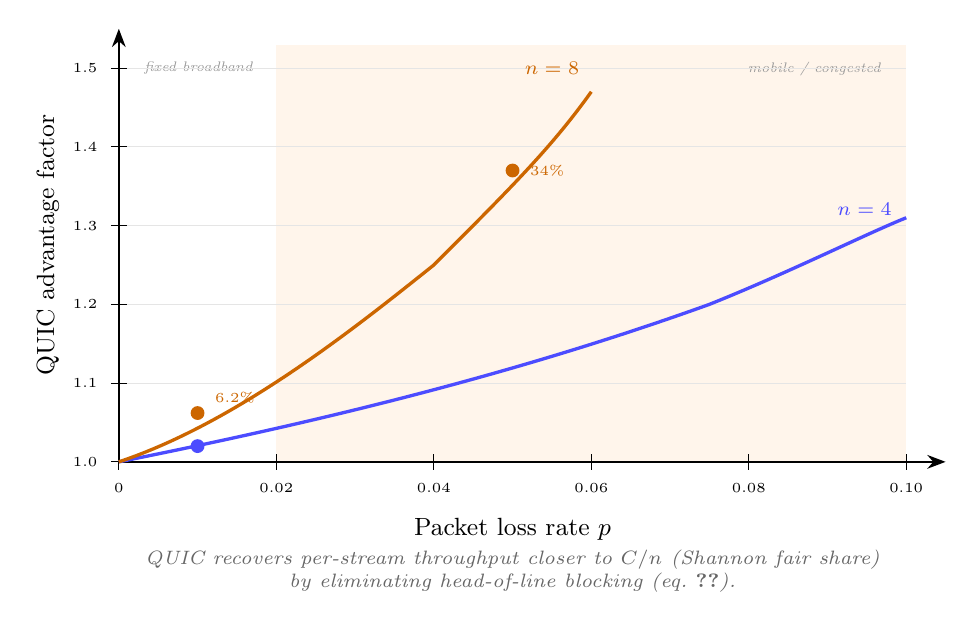
\begin{tikzpicture}[>=Stealth]

% --- Shaded region (drawn FIRST so curves appear on top) ---
\fill[orange!8] (2, 0) rectangle (10, 5.3);
\node[font=\tiny\itshape, text=black!40, anchor=north east] at (9.8, 5.2)
  {mobile / congested};
\node[font=\tiny\itshape, text=black!40, anchor=north west] at (0.2, 5.2)
  {fixed broadband};

% --- Grid lines ---
\foreach \y in {1, 2, 3, 4, 5} {
  \draw[gray!20] (0, \y) -- (10, \y);
}

% --- Axes ---
\draw[->, thick] (0, 0) -- (10.5, 0);
\draw[->, thick] (0, 0) -- (0, 5.5);

% --- Axis titles (positioned to clear tick labels) ---
\node[font=\small] at (5, -0.85) {Packet loss rate $p$};
\node[font=\small, rotate=90] at (-0.9, 2.75) {QUIC advantage factor};

% --- X-axis labels ---
\foreach \x/\lab in {0/0, 2/0.02, 4/0.04, 6/0.06, 8/0.08, 10/0.10} {
  \draw (\x, -0.1) -- (\x, 0.1);
  \node[font=\tiny, anchor=north] at (\x, -0.15) {\lab};
}

% --- Y-axis labels ---
\foreach \y/\lab in {0/1.0, 1/1.1, 2/1.2, 3/1.3, 4/1.4, 5/1.5} {
  \draw (-0.1, \y) -- (0.1, \y);
  \node[font=\tiny, anchor=east] at (-0.15, \y) {\lab};
}

% --- n=4 curve: 1/(1-p)^2 ---
\draw[very thick, blue!70]
  (0, 0) .. controls (2.5, 0.5) and (5, 1.1) ..
  (7.5, 2.0) .. controls (8.5, 2.4) and (9.5, 2.9) ..
  (10, 3.1);
\node[font=\scriptsize, blue!70, anchor=south west] at (9.0, 3.0)
  {$n = 4$};

% --- n=8 curve: 1/(1-p)^6 ---
\draw[very thick, orange!80!black]
  (0, 0) .. controls (1.5, 0.5) and (3, 1.7) ..
  (4, 2.5) .. controls (5, 3.5) and (5.5, 4.0) ..
  (6, 4.7);
\node[font=\scriptsize, orange!80!black, anchor=south] at (5.5, 4.8)
  {$n = 8$};

% --- Reference points ---
\fill[orange!80!black] (1.0, 0.62) circle (2.5pt);
\node[font=\tiny, orange!80!black, anchor=south west] at (1.1, 0.62)
  {6.2\%};

\fill[orange!80!black] (5.0, 3.7) circle (2.5pt);
\node[font=\tiny, orange!80!black, anchor=west] at (5.1, 3.7)
  {34\%};

\fill[blue!70] (1.0, 0.20) circle (2.5pt);

% --- Annotation ---
\node[font=\scriptsize\itshape, text=black!60, align=center,
  anchor=north] at (5.0, -1.0)
  {QUIC recovers per-stream throughput closer to $C/n$ (Shannon fair share)\\
   by eliminating head-of-line blocking (eq.~\ref{eq:hol-ratio}).};

\end{tikzpicture}
\caption{QUIC advantage factor $1/(1-p)^{n-2}$ over TCP for multiplexed
  streams. At 5\% loss with $n=8$ streams, QUIC delivers 34\% more
  per-stream throughput by maintaining independence at the transport layer.}
\label{fig:hol-blocking}
\end{figure}

\subsubsection{Connection Establishment Latency}

Let $\tau$ denote the one-way latency (half the round-trip time). The
information-carrying capacity during connection establishment is zero;
the handshake represents pure overhead. The time to first useful byte
is:
\begin{align}
  T_{\text{TCP+TLS\,1.3}} &= 2\tau_{\text{TCP}} + \tau_{\text{TLS}}
    = 3\tau \quad \text{(1-RTT TLS~1.3)} \label{eq:tcp-setup} \\
  T_{\text{QUIC}} &= \tau \quad \text{(1-RTT)}
    \label{eq:quic-setup} \\
  T_{\text{QUIC,\,0-RTT}} &= 0 \quad \text{(resumption)}
    \label{eq:quic-0rtt}
\end{align}
The QUIC 0-RTT case (\ref{eq:quic-0rtt}) eliminates the handshake
entirely for resumed connections. The information lost during
handshake dead time, relative to steady-state capacity, is:
\begin{equation}
  I_{\text{lost}} = C_{\text{link}} \cdot T_{\text{setup}}
  \label{eq:ilost}
\end{equation}
For a 120~Mbps link with $\tau = 25$~ms (typical fixed broadband in
2026), the TCP+TLS~1.3 handshake wastes $120 \times 10^6 \times 0.075
= 9 \times 10^6$ bits (1.125~MB), while QUIC~1-RTT wastes only
$3 \times 10^6$ bits (375~KB).

\subsection{Source Coding Efficiency}

The rate-distortion function $R(D)$ defines the minimum bit rate
required to represent a source at distortion level $D$. For a
Gaussian source with variance $\sigma^2$ under mean squared error
distortion:
\begin{equation}
  R(D) = \frac{1}{2} \log_2 \frac{\sigma^2}{D}
    \quad \text{[bits/sample]}
  \label{eq:rate-distortion}
\end{equation}

\excursus{Excursus: Why Gaussian source?}{The Gaussian memoryless model is used
because it yields the highest (worst-case) $R(D)$ among all sources of equal
variance. Any codec that approaches the Gaussian bound on real video is
therefore doing at least as well as the bound predicts --- the true $R(D)$ for
spatially and temporally correlated video lies below the Gaussian curve, making
it a conservative benchmark.}

No practical codec achieves $R(D)$;\footnote{The $R(D)$ curve in
Figure~\ref{fig:rate-distortion} is the Gaussian memoryless source bound
(equation~\ref{eq:rate-distortion}), which is an upper bound on the true
$R(D)$ for non-Gaussian sources such as video.  Additionally, $R(D)$ assumes
zero excess-distortion probability, whereas practical codecs permit a
frame-level excess-distortion probability on the order of $10^{-6}$ to
$10^{-8}$.  Both factors allow codec operating points measured on real content
to approach or marginally cross the Gaussian bound.} real codecs operate at
some rate $R_{\text{codec}} > R(D)$. We define the coding efficiency gap as:
\begin{equation}
  \Delta = \frac{R_{\text{codec}} - R(D)}{R(D)}
  \label{eq:coding-gap}
\end{equation}

The codecs in the WebRTC stack can be ordered by their empirical
proximity to $R(D)$ for typical video content at conversational
resolutions (720p, 30~fps). Using published Bj\o ntegaard Delta (BD)
rate measurements:
\begin{equation}
  R_{\text{H.264}} > R_{\text{VP9}} > R_{\text{AV1}}
    > R(D)
  \label{eq:codec-ordering}
\end{equation}

Specifically, the empirical rate savings at equivalent PSNR are
approximately:
\begin{align}
  R_{\text{VP9}}  &\approx 0.65 \cdot R_{\text{H.264}}
    \quad (\sim\!35\% \text{ savings}) \label{eq:vp9-savings} \\
  R_{\text{AV1}}  &\approx 0.70 \cdot R_{\text{VP9}}
    \approx 0.46 \cdot R_{\text{H.264}}
    \quad (\sim\!30\% \text{ over VP9})
  \label{eq:av1-savings}
\end{align}

\begin{figure}[ht]
\centering
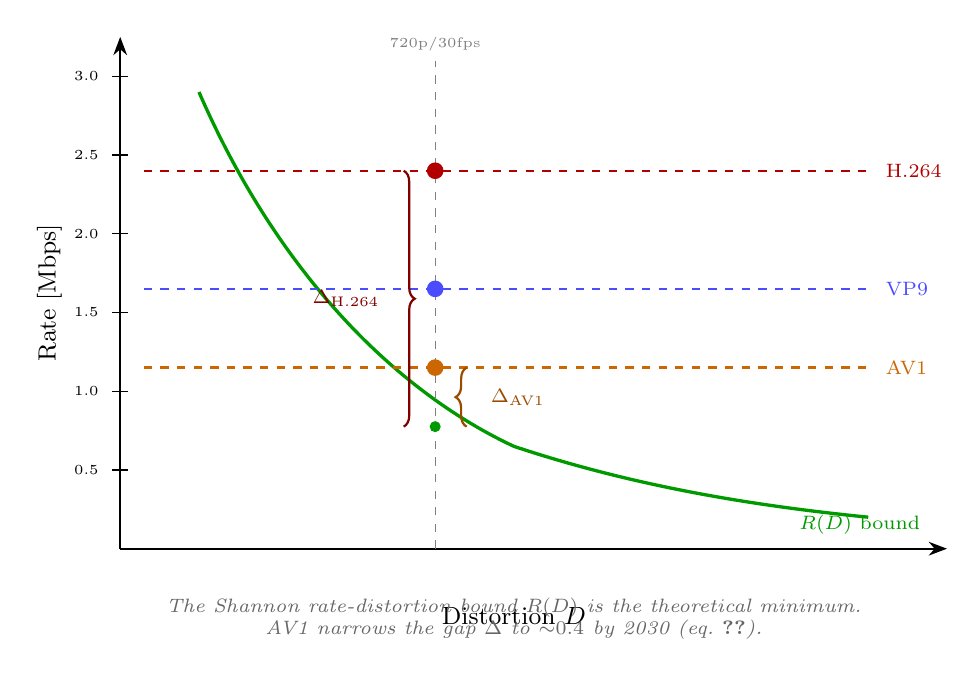
\begin{tikzpicture}[>=Stealth]

% --- Axes ---
\draw[->, thick] (0, 0) -- (10.5, 0);
\draw[->, thick] (0, 0) -- (0, 6.5);

% --- Axis titles ---
\node[font=\small] at (5, -0.85) {Distortion $D$};
\node[font=\small, rotate=90] at (-0.9, 3.25) {Rate [Mbps]};

% --- Y-axis rate labels ---
\foreach \y/\lab in {1.0/0.5, 2.0/1.0, 3.0/1.5, 4.0/2.0, 5.0/2.5, 6.0/3.0} {
  \draw (-0.1, \y) -- (0.1, \y);
  \node[font=\tiny, anchor=east] at (-0.15, \y) {\lab};
}

% --- R(D) Shannon bound curve ---
\draw[very thick, green!60!black]
  (1.0, 5.8) .. controls (2.0, 3.5) and (3.5, 2.0) ..
  (5.0, 1.3) .. controls (6.5, 0.8) and (8.0, 0.55) ..
  (9.5, 0.4);
\node[font=\scriptsize, green!60!black, anchor=north west] at (8.5, 0.55)
  {$R(D)$ bound};

% --- Reference distortion line (720p/30fps operating point) ---
\draw[thin, gray, dashed] (4.0, 0) -- (4.0, 6.2);
\node[font=\tiny, gray, anchor=south] at (4.0, 6.2) {720p/30fps};

% --- R(D) value at reference distortion ---
\fill[green!60!black] (4.0, 1.55) circle (2pt);

% --- Codec operating points at reference distortion ---
% H.264: ~2.5 Mbps
\draw[thick, dashed, red!70!black] (0.3, 4.8) -- (9.5, 4.8);
\fill[red!70!black] (4.0, 4.8) circle (3pt);
\node[font=\scriptsize, red!70!black, anchor=west] at (9.6, 4.8) {H.264};

% VP9: ~1.6 Mbps (0.65 * H.264)
\draw[thick, dashed, blue!70] (0.3, 3.3) -- (9.5, 3.3);
\fill[blue!70] (4.0, 3.3) circle (3pt);
\node[font=\scriptsize, blue!70, anchor=west] at (9.6, 3.3) {VP9};

% AV1: ~1.15 Mbps (0.46 * H.264)
\draw[thick, dashed, orange!80!black] (0.3, 2.3) -- (9.5, 2.3);
\fill[orange!80!black] (4.0, 2.3) circle (3pt);
\node[font=\scriptsize, orange!80!black, anchor=west] at (9.6, 2.3) {AV1};

% --- Gap annotations (braces) ---
% H.264 gap
\draw[decorate, decoration={brace, amplitude=4pt, mirror},
  thick, red!50!black]
  (3.6, 1.55) -- (3.6, 4.8)
  node[midway, anchor=east, font=\scriptsize, xshift=-5pt]
  {$\Delta_{\text{H.264}}$};

% AV1 gap
\draw[decorate, decoration={brace, amplitude=4pt},
  thick, orange!60!black]
  (4.4, 1.55) -- (4.4, 2.3)
  node[midway, anchor=west, font=\scriptsize, xshift=5pt]
  {$\Delta_{\text{AV1}}$};

% --- Annotation ---
\node[font=\scriptsize\itshape, text=black!60, align=center,
  anchor=north] at (5.0, -0.5)
  {The Shannon rate-distortion bound $R(D)$ is the theoretical minimum.\\
   AV1 narrows the gap $\Delta$ to ${\sim}0.4$ by 2030 (eq.~\ref{eq:coding-gap}).};

\end{tikzpicture}
\caption{Codec operating rates vs.\ the Shannon rate-distortion bound $R(D)$
  at 720p/30fps. Each codec operates above the theoretical minimum; the gap
  $\Delta$ (eq.~\ref{eq:coding-gap}) shrinks from H.264 through VP9 to AV1,
  approaching but never reaching the bound.}
\label{fig:rate-distortion}
\end{figure}

\subsubsection{Codec Entropy and WebCodecs}

The WebCodecs API (W3C Working Draft) exposes per-frame codec access,
allowing measurement and control of the instantaneous encoding rate.
For a video frame $f_t$ at time $t$, the encoder output has empirical
entropy:
\begin{equation}
  \hat{H}(f_t) = -\sum_{s \in \mathcal{S}}
    p(s \mid f_t) \log_2 p(s \mid f_t)
  \label{eq:frame-entropy}
\end{equation}
where $\mathcal{S}$ is the set of symbols emitted by the entropy coder
(CABAC for H.264/AV1, arithmetic coding for VP9). WebCodecs enables
applications to observe $|E(f_t)|$ (the encoded frame size in bits)
directly, which serves as a practical upper bound on
$\hat{H}(f_t)$:
\begin{equation}
  \hat{H}(f_t) \leq |E(f_t)| \leq R_{\text{codec}} / \text{fps}
  \label{eq:entropy-bound}
\end{equation}

\subsection{Effective Information Rate by Time Horizon}

We now combine transport and source coding measures to estimate the
effective information rate for a representative real-time video
session: a single 720p/30fps video call with one audio channel.

\excursus{Excursus: Why 720p?}{Throughout this appendix, 720p/30fps is used as
a fixed reference for cross-era comparison, not as a prediction that 720p
remains the dominant conferencing resolution. The bandwidth surplus quantified
below is precisely what enables migration to 1080p (feasible by ${\sim}$2028
with AV1 hardware encode at today's 720p bit rates) and 4K (feasible by
${\sim}$2030). The 720p baseline makes the efficiency gains legible: the same
task gets cheaper, freeing capacity for higher quality or more streams.}

Define the \emph{net information rate} as:
\begin{equation}
  I_{\text{net}} = R_{\text{codec}} \cdot \eta_{\text{transport}}
    \cdot (1 - \rho_{\text{overhead}})
    \cdot (1 - p_{\text{loss}})
  \label{eq:inet}
\end{equation}

\begin{table}[ht]
\centering
\small
\renewcommand{\arraystretch}{1.4}
\begin{tabularx}{\textwidth}{lXXX}
\toprule
\textbf{Parameter} & \textbf{March 2026} & \textbf{2027--2028} &
  \textbf{2029--2031} \\
\midrule
Median link capacity &
  120~Mbps &
  $\sim$150~Mbps &
  200--300~Mbps \\
Dominant codec (WebRTC) &
  VP9 / H.264 &
  VP9 / AV1 (HW) &
  AV1 (HW default) \\
Codec rate (720p/30fps) &
  1.5--2.5~Mbps &
  1.0--1.8~Mbps &
  0.7--1.2~Mbps \\
$\eta_{\text{transport}}$ &
  0.92 (QUIC) &
  0.93 &
  0.94 \\
$\rho_{\text{overhead}}$ (SRTP+QUIC) &
  0.06 &
  0.05 &
  0.04 \\
Typical loss $p$ &
  0.01--0.03 &
  0.01--0.02 &
  0.005--0.01 \\
$I_{\text{net}}$ (720p video) &
  1.3--2.2~Mbps &
  0.9--1.6~Mbps &
  0.6--1.1~Mbps \\
$I_{\text{net}}$ as \% of $C_{\text{link}}$ &
  1.1--1.8\% &
  0.6--1.1\% &
  0.2--0.6\% \\
\bottomrule
\end{tabularx}
\caption{Effective information rate for a 720p/30fps WebRTC video stream.
  The declining ratio $I_{\text{net}} / C_{\text{link}}$ reflects both
  improved codec efficiency and growing link capacity, freeing bandwidth
  for higher resolutions, additional streams, or concurrent data
  channels.}
\label{tab:inet}
\end{table}

The declining ratio $I_{\text{net}} / C_{\text{link}}$ in
Table~\ref{tab:inet} is the central quantitative observation: by 2030, a
720p video call consumes less than 0.5\% of available link capacity. The
surplus capacity enables qualitative changes --- 4K video conferencing,
multi-stream layouts, or concurrent data channels via WebTransport ---
that are quantitatively infeasible in 2026.

\begin{figure}[ht]
\centering
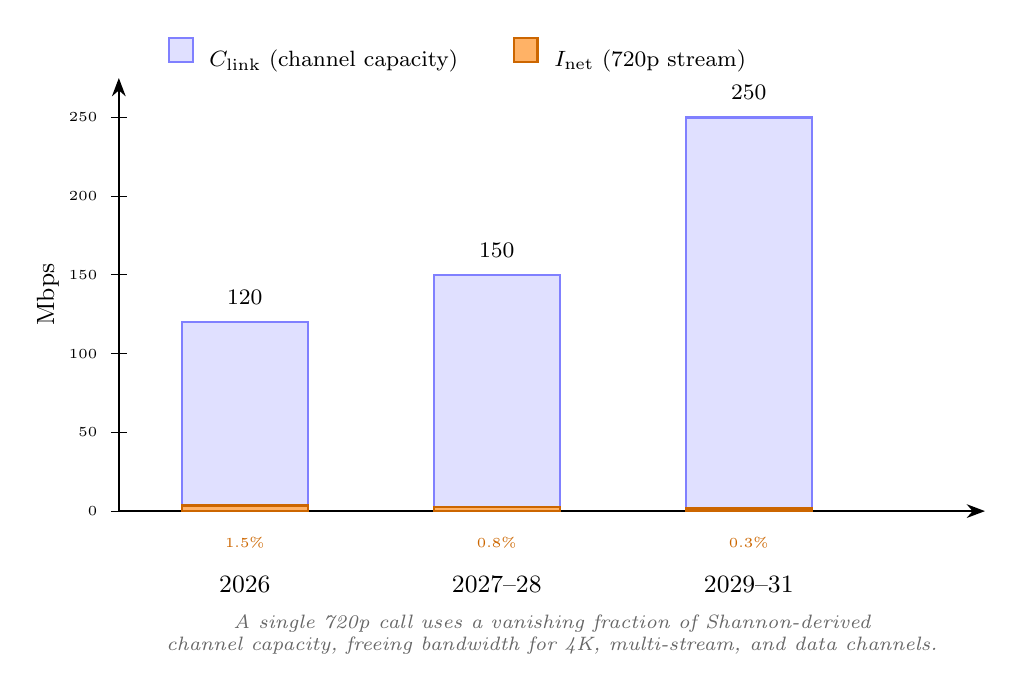
\begin{tikzpicture}[>=Stealth]

% --- Axes ---
\draw[->, thick] (0, 0) -- (11, 0);
\draw[->, thick] (0, 0) -- (0, 5.5);

% --- Axis title ---
\node[font=\small, rotate=90] at (-0.9, 2.75) {Mbps};

% --- Y-axis labels ---
\foreach \y/\lab in {0/0, 1/50, 2/100, 3/150, 4/200, 5/250} {
  \draw (-0.1, \y) -- (0.1, \y);
  \node[font=\tiny, anchor=east] at (-0.15, \y) {\lab};
}

% --- Group: March 2026 ---
% C_link = 120 Mbps -> y = 2.4
\fill[blue!12] (0.8, 0) rectangle (2.4, 2.4);
\draw[blue!50, thick] (0.8, 0) rectangle (2.4, 2.4);
% I_net = 1.75 Mbps (midpoint) -> y = 0.035
\fill[orange!60] (0.8, 0) rectangle (2.4, 0.07);
\draw[orange!80!black, thick] (0.8, 0) rectangle (2.4, 0.07);
\node[font=\footnotesize, anchor=south] at (1.6, 2.5) {120};
\node[font=\tiny, orange!80!black] at (1.6, -0.4) {1.5\%};
\node[font=\small, anchor=north] at (1.6, -0.7) {2026};

% --- Group: 2027--2028 ---
% C_link = 150 Mbps -> y = 3.0
\fill[blue!12] (4.0, 0) rectangle (5.6, 3.0);
\draw[blue!50, thick] (4.0, 0) rectangle (5.6, 3.0);
% I_net = 1.25 Mbps (midpoint) -> y = 0.025
\fill[orange!60] (4.0, 0) rectangle (5.6, 0.05);
\draw[orange!80!black, thick] (4.0, 0) rectangle (5.6, 0.05);
\node[font=\footnotesize, anchor=south] at (4.8, 3.1) {150};
\node[font=\tiny, orange!80!black] at (4.8, -0.4) {0.8\%};
\node[font=\small, anchor=north] at (4.8, -0.7) {2027--28};

% --- Group: 2029--2031 ---
% C_link = 250 Mbps -> y = 5.0
\fill[blue!12] (7.2, 0) rectangle (8.8, 5.0);
\draw[blue!50, thick] (7.2, 0) rectangle (8.8, 5.0);
% I_net = 0.85 Mbps (midpoint) -> y = 0.017
\fill[orange!60] (7.2, 0) rectangle (8.8, 0.034);
\draw[orange!80!black, thick] (7.2, 0) rectangle (8.8, 0.034);
\node[font=\footnotesize, anchor=south] at (8.0, 5.1) {250};
\node[font=\tiny, orange!80!black] at (8.0, -0.4) {0.3\%};
\node[font=\small, anchor=north] at (8.0, -0.7) {2029--31};

% --- Legend ---
\node[anchor=west, font=\footnotesize] at (0.5, 5.8) {%
  \tikz[baseline=-0.5ex]{\fill[blue!12] (0,0) rectangle (0.3,0.3);
    \draw[blue!50, thick] (0,0) rectangle (0.3,0.3);}
  ~$C_{\text{link}}$ (channel capacity) \qquad
  \tikz[baseline=-0.5ex]{\fill[orange!60] (0,0) rectangle (0.3,0.3);
    \draw[orange!80!black, thick] (0,0) rectangle (0.3,0.3);}
  ~$I_{\text{net}}$ (720p stream)};

% --- Annotation ---
\node[font=\scriptsize\itshape, text=black!60, align=center,
  anchor=north] at (5.5, -1.2)
  {A single 720p call uses a vanishing fraction of Shannon-derived\\
   channel capacity, freeing bandwidth for 4K, multi-stream, and data channels.};

\end{tikzpicture}
\caption{Channel capacity $C_{\text{link}}$ vs.\ effective information rate
  $I_{\text{net}}$ for a single 720p/30fps stream across time horizons. The
  orange bar (stream rate) is barely visible against the blue bar (capacity),
  illustrating the growing surplus as codecs improve and bandwidth increases.}
\label{fig:inet-capacity}
\end{figure}

\subsection{Security Entropy and Key Space}

The DTLS-SRTP security architecture (RFCs~8827, 3711) protects all
WebRTC media. Information-theoretic security requires that the key
entropy exceed the information content of the protected material.

For a DTLS~1.3 handshake with ECDHE on P-256, the key agreement
provides:
\begin{equation}
  H_{\text{key}} = 128 \text{~bits of security}
  \label{eq:key-entropy}
\end{equation}

The SRTP master key is 128 bits (AES-128-GCM), giving an exhaustive
search cost of $2^{128}$ operations. The total information content of a
one-hour 720p video call at 2~Mbps is:
\begin{equation}
  I_{\text{call}} = 2 \times 10^6 \times 3600
    = 7.2 \times 10^9 \text{~bits}
    \approx 2^{32.7} \text{~bits}
  \label{eq:call-content}
\end{equation}

The ratio of key entropy to protected content:
\begin{equation}
  \frac{H_{\text{key}}}{I_{\text{call}}}
    = \frac{128}{32.7} \approx 3.91
  \label{eq:security-margin}
\end{equation}

This ratio remains comfortably above~1 even for much longer sessions.
For a continuous 24-hour 4K AV1 stream at 15~Mbps:
\begin{equation}
  I_{\text{stream}} = 15 \times 10^6 \times 86400
    = 1.296 \times 10^{12} \text{~bits}
    \approx 2^{40.2} \text{~bits}
\end{equation}
yielding $H_{\text{key}} / I_{\text{stream}} \approx 3.18$, still
well above the threshold.

\subsubsection{End-to-End Encryption via Encoded Transforms}

The RTCRtpScriptTransform API (Encoded Transforms) enables
application-layer E2EE within the WebRTC pipeline. From an
information-theoretic perspective, this introduces a second encryption
layer with its own key, creating a \emph{nested channel}:
\begin{equation}
  X \xrightarrow{\;K_{\text{E2EE}}\;}
  E_1(X) \xrightarrow{\;K_{\text{SRTP}}\;}
  E_2(E_1(X))
  \label{eq:nested}
\end{equation}

The mutual information between the ciphertext and plaintext, given
neither key, satisfies:
\begin{equation}
  I\!\left(X;\, E_2(E_1(X))\right) \leq
    \min\!\big(H(K_{\text{E2EE}})^{-1},\;
    H(K_{\text{SRTP}})^{-1}\big)
    \cdot I_{\text{call}}
  \label{eq:mutual-e2ee}
\end{equation}

In practice, with $H(K_{\text{E2EE}}) = H(K_{\text{SRTP}}) = 128$
bits, this quantity is negligible ($\ll 1$ bit for any practical
session length), confirming that the nested encryption provides
information-theoretic confidentiality well beyond computational
security guarantees.

Today (March~2026), Encoded Transforms remain Chrome-only. By
2027--2028 (Section~8.3), cross-browser standardization will make
this nested channel universally available. By 2029--2031, SFrame
for group calls will extend this to $n$-party sessions, where the
mutual information between any non-member and the group plaintext
remains negligible:
\begin{equation}
  I\!\left(X;\, E(X) \;\middle|\; K_i \notin
    \{K_1, \ldots, K_n\}\right) \approx 0
  \label{eq:sframe}
\end{equation}

\subsection{WebTransport: Unreliable Datagrams and Channel Capacity}

WebTransport (RFC~9297) introduces unreliable datagrams to browser-server
communication. For latency-sensitive applications (game state, sensor
telemetry), the relevant measure is not throughput but
\emph{freshness-weighted information rate}. Define the value of a
datagram as exponentially decaying with delivery latency $\delta$:
\begin{equation}
  V(\delta) = e^{-\lambda \delta}
  \label{eq:freshness}
\end{equation}
where $\lambda > 0$ is an application-specific decay rate. The
effective information rate under unreliable delivery is:
\begin{equation}
  I_{\text{WT}} = R_{\text{send}} \cdot (1 - p_{\text{loss}})
    \cdot \mathbb{E}\!\left[e^{-\lambda \delta}\right]
  \label{eq:iwt}
\end{equation}

Under reliable delivery (TCP/WebSocket), a retransmission delays
subsequent data, so:
\begin{equation}
  I_{\text{WS}} = R_{\text{send}}
    \cdot \mathbb{E}\!\left[e^{-\lambda(\delta + p \cdot 2\tau)}\right]
  \label{eq:iws}
\end{equation}

The ratio $I_{\text{WT}} / I_{\text{WS}}$ exceeds 1 when:
\begin{equation}
  (1 - p) \cdot e^{\lambda \cdot p \cdot 2\tau} > 1
  \quad \Longleftrightarrow \quad
  \lambda > \frac{-\ln(1 - p)}{2 p \tau}
  \label{eq:wt-advantage}
\end{equation}

For $p = 0.02$ and $\tau = 25$~ms, this gives $\lambda > 20.2$~s$^{-1}$
(half-life $< 34$~ms).

\excursus{Excursus: Why $p = 0.02$ and $\tau = 25$\,ms?}{These values represent
median fixed-broadband conditions in 2026 (Table~\ref{tab:inet}). On mobile or
congested links ($p \approx 0.05$, $\tau \approx 50$\,ms), the threshold
$\lambda^*$ drops to ${\sim}10$\,s$^{-1}$, broadening WebTransport's advantage
to applications with data half-lives up to ${\sim}70$\,ms. The fixed-broadband
reference is thus conservative: mobile scenarios favor unreliable delivery even
more strongly.}

Any application where data older than
$\sim$30~ms is useless benefits from WebTransport's unreliable
mode over WebSocket --- precisely the regime of interactive gaming, live
cursor tracking, and real-time sensor feeds.

As of March~2026, Safari does not support WebTransport
(Section~5), limiting coverage to $\sim$82\%. By 2027--2028
(Section~8.2), universal support will allow applications to rely on
(\ref{eq:iwt}) without fallback paths.

\begin{figure}[ht]
\centering
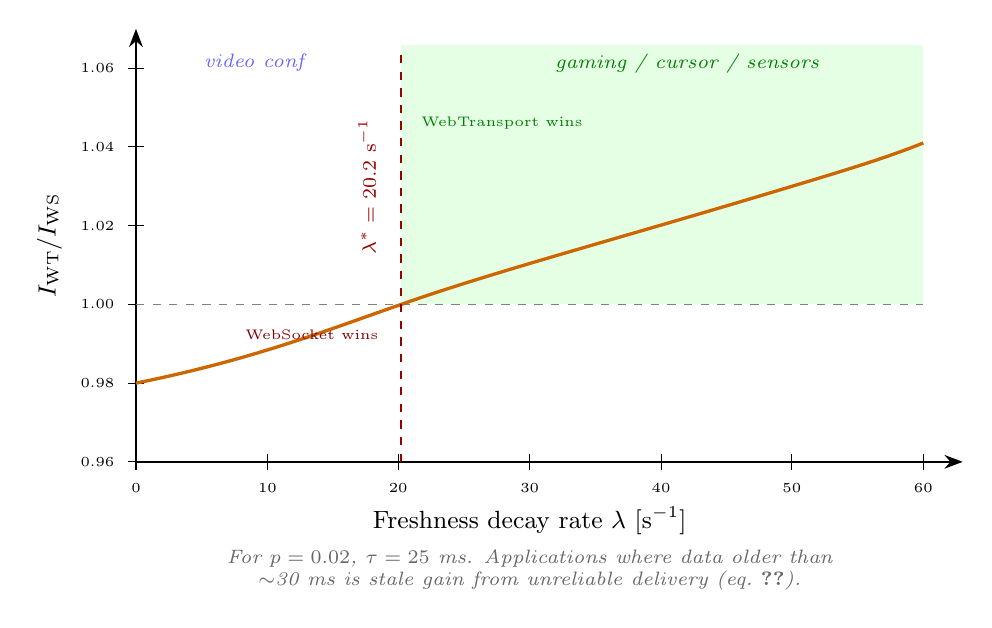
\begin{tikzpicture}[>=Stealth]

% --- Axes ---
\draw[->, thick] (0, 0) -- (10.5, 0);
\draw[->, thick] (0, 0) -- (0, 5.5);

% --- Axis titles (positioned to clear tick labels) ---
\node[font=\small] at (5, -0.75)
  {Freshness decay rate $\lambda$ [s$^{-1}$]};
\node[font=\small, rotate=90] at (-1.1, 2.75)
  {$I_{\text{WT}} / I_{\text{WS}}$};

% --- X-axis labels ---
\foreach \x/\lab in {0/0, 1.67/10, 3.33/20, 5.0/30, 6.67/40, 8.33/50, 10/60} {
  \draw (\x, -0.1) -- (\x, 0.1);
  \node[font=\tiny, anchor=north] at (\x, -0.15) {\lab};
}

% --- Y-axis labels (0.96 to 1.06, each 0.02 = 1 unit) ---
\foreach \y/\lab in {0/0.96, 1/0.98, 2/1.00, 3/1.02, 4/1.04, 5/1.06} {
  \draw (-0.1, \y) -- (0.1, \y);
  \node[font=\tiny, anchor=east] at (-0.15, \y) {\lab};
}

% --- Ratio = 1.0 line (y=2 maps to ratio 1.0) ---
\draw[thin, gray, dashed] (0, 2) -- (10, 2);

% --- Shade WebTransport advantage region ---
% lambda* = 20.2 -> x = 3.37
\fill[green!10] (3.37, 2) rectangle (10, 5.3);

% --- I_WT/I_WS curve: 0.98*exp(lambda*0.001) ---
% Y range: 0.96-1.06 (each 0.02 = 1 unit). lambda=0: y=1, lambda*=20.2: y=2, lambda=60: y=4.05
\draw[very thick, orange!80!black]
  (0, 1.0) .. controls (1.5, 1.3) and (2.5, 1.7) ..
  (3.37, 2.0) .. controls (4.5, 2.4) and (6, 2.8) ..
  (8, 3.4) .. controls (9, 3.7) and (9.5, 3.85) ..
  (10, 4.05);

% --- Threshold line ---
\draw[thick, dashed, red!60!black] (3.37, 0) -- (3.37, 5.2);
\node[font=\scriptsize, red!60!black, anchor=south, rotate=90] at (3.17, 3.5)
  {$\lambda^* = 20.2$ s$^{-1}$};

% --- Application regime labels ---
\node[font=\scriptsize\itshape, text=blue!60, anchor=north] at (1.5, 5.3)
  {video conf};
\node[font=\scriptsize\itshape, text=green!50!black, anchor=north] at (7.0, 5.3)
  {gaming / cursor / sensors};

% --- Mark advantage/disadvantage ---
\node[font=\tiny, text=red!50!black, anchor=north east] at (3.2, 1.8)
  {WebSocket wins};
\node[font=\tiny, text=green!50!black, anchor=north west] at (3.5, 4.5)
  {WebTransport wins};

% --- Annotation ---
\node[font=\scriptsize\itshape, text=black!60, align=center,
  anchor=north] at (5.0, -1.0)
  {For $p = 0.02$, $\tau = 25$~ms. Applications where data older than\\
   ${\sim}$30~ms is stale gain from unreliable delivery (eq.~\ref{eq:wt-advantage}).};

\end{tikzpicture}
\caption{Freshness-weighted information rate ratio $I_{\text{WT}} / I_{\text{WS}}$
  as a function of decay rate $\lambda$. Above the threshold $\lambda^*$,
  WebTransport's unreliable datagrams deliver more useful information per
  unit time than WebSocket's reliable delivery, because retransmission
  wastes capacity on stale data.}
\label{fig:freshness}
\end{figure}

\subsection{Projections Summary and Practical Implications}

\begin{table}[ht]
\centering
\small
\renewcommand{\arraystretch}{1.4}
\begin{tabularx}{\textwidth}{lXXX}
\toprule
\textbf{Measure} & \textbf{March 2026} & \textbf{2027--2028} &
  \textbf{2029--2031} \\
\midrule
Channel capacity $C_{\text{link}}$ &
  120~Mbps &
  150~Mbps &
  250~Mbps \\
HOL blocking factor $(1\!-\!p)^{n-2}$ at $n\!=\!8$ &
  0.94 ($p\!=\!0.01$) &
  0.94 &
  0.97 ($p\!=\!0.005$) \\
Source coding gap $\Delta$ &
  VP9: $\sim$0.8 &
  AV1 HW: $\sim$0.5 &
  AV1 opt: $\sim$0.4 \\
$I_{\text{net}}$ per 720p stream &
  1.3--2.2~Mbps &
  0.9--1.6~Mbps &
  0.6--1.1~Mbps \\
Max 720p streams in $C_{\text{link}}$ &
  $\sim$55--90 &
  $\sim$95--165 &
  $\sim$230--415 \\
E2EE availability &
  Chrome only &
  Cross-browser &
  SFrame $n$-party \\
WebTransport coverage &
  82\% &
  $\sim$100\% &
  100\% \\
Freshness threshold $\lambda^*$ &
  20.2~s$^{-1}$ &
  $\sim$18~s$^{-1}$ &
  $\sim$15~s$^{-1}$ \\
\bottomrule
\end{tabularx}
\caption{Information-theoretic measures across time horizons. $\Delta$
  is the coding efficiency gap (\ref{eq:coding-gap}), $I_{\text{net}}$
  is the net information rate (\ref{eq:inet}), and $\lambda^*$ is the
  freshness decay threshold above which WebTransport dominates WebSocket
  (\ref{eq:wt-advantage}).}
\label{tab:projections}
\end{table}

The trajectory is clear: the combination of improving source coding
(AV1 hardware), expanding channel capacity (broadband growth), and
maturing transport protocols (QUIC universal, WebTransport universal)
drives the \emph{information cost per unit of communicated experience}
steadily downward. The remaining question is not whether the
Shannon capacity suffices --- it already does, by orders of magnitude
--- but how efficiently the protocol stack converts that capacity into
delivered, fresh, secure information at the application layer. By
2030, the gap between theoretical capacity and realized throughput will
be the narrowest it has ever been for browser-based real-time
communication.

\subsubsection{What the Theory Means for Applications}

The equations and figures in this appendix are not purely academic. Each
theoretical result maps to a concrete design decision that application
developers face today and over the next five years.

\textbf{Codec selection determines bandwidth cost, not quality.}
The rate-distortion analysis (Section~A.2, Figure~\ref{fig:rate-distortion})
shows that AV1 operates at roughly 46\% of H.264's bit rate for equivalent
perceptual quality at 720p. In practice, this means a WebRTC application
switching from H.264 to AV1 can either halve its bandwidth consumption at
the same quality or substantially increase resolution (e.g., 720p to 1080p)
within the same bandwidth envelope. By 2030, with AV1 hardware encoding
ubiquitous and the coding gap $\Delta$ approaching 0.4, further codec
improvements yield diminishing returns --- the stack will be operating close
enough to the Shannon rate-distortion bound that the next generation of
efficiency gains will come from transport and architecture, not codecs alone.

\textbf{QUIC's advantage is situational but decisive on bad networks.}
The head-of-line blocking analysis (Section~A.1.1,
Figure~\ref{fig:hol-blocking}) shows that QUIC's per-stream throughput
advantage over TCP is modest on good networks (6\% at 1\% loss) but
substantial on degraded ones (34\% at 5\% loss). The practical implication
is that applications targeting mobile users, emerging markets, or congested
enterprise networks --- precisely the environments where real-time
communication is hardest --- benefit disproportionately from QUIC-based
transports. For a video conference with 8 participants on a cellular
connection experiencing 3--5\% packet loss, the difference between QUIC and
TCP is the difference between usable and degraded video.

\textbf{Connection latency is a solved problem for returning users.}
The handshake analysis (Section~A.1.2) shows that QUIC 0-RTT eliminates
connection establishment overhead entirely for resumed connections. For a
WebTransport application that a user opens daily --- a collaboration tool,
a live dashboard, a recurring meeting client --- the time to first useful
byte drops to zero. The 1.125~MB of wasted capacity during a TCP+TLS
handshake on a 120~Mbps link may seem small, but for latency-sensitive
applications where the first 100~ms of perceived responsiveness determines
user experience, the difference is measurable.

\textbf{Bandwidth surplus enables architectural ambition.}
The effective information rate analysis (Section~A.3,
Figure~\ref{fig:inet-capacity}) reveals the most consequential practical
finding: a single 720p video stream consumes a vanishing fraction of
available link capacity (under 0.5\% by 2030). This surplus is not merely
``headroom'' --- it is the resource that makes new application architectures
feasible. A 250~Mbps link can theoretically carry 230--415 simultaneous 720p
streams. In practice, this means applications can afford to run multiple
concurrent media flows (video, screen share, spatial audio), data channels
(collaborative editing, file transfer), and telemetry streams without
contending for bandwidth. The constraint shifts from ``can the network carry
this?''\ to ``can the application manage this complexity?''

\textbf{End-to-end encryption adds negligible overhead.}
The security analysis (Section~A.4) confirms that the nested DTLS-SRTP plus
E2EE architecture imposes no meaningful information-theoretic cost. The key
entropy ($2^{128}$) exceeds the information content of any practical session
by a factor of at least 3. For application developers, this means E2EE can
be treated as a default rather than a premium feature --- there is no
bandwidth, latency, or capacity penalty for encrypting at the application
layer on top of the transport-layer encryption that WebRTC already mandates.
The only constraint is API availability, which moves from Chrome-only (2026)
to universal (2028).

\textbf{WebTransport unlocks real-time data that WebSocket cannot serve.}
The freshness analysis (Section~A.5, Figure~\ref{fig:freshness}) quantifies
when unreliable delivery outperforms reliable delivery: any data with a
useful half-life below approximately 34~ms benefits from WebTransport's
unreliable datagrams. This covers a wide class of interactive applications
--- game state synchronization, live cursor and pointer sharing, real-time
sensor feeds, collaborative whiteboard strokes --- where retransmitting a
stale update is worse than dropping it. Before WebTransport, these
applications had to choose between WebSocket (reliable but stale under loss)
and WebRTC DataChannel (unreliable mode available but requiring the full
peer-to-peer ICE/DTLS machinery). WebTransport provides the unreliable
mode with a simple client-server model over HTTP/3, removing the
architectural overhead.

\textbf{The overall picture: the stack converges on efficiency.}
Taken together, the information-theoretic measures trace a consistent
trajectory. The protocol stack is converging toward the theoretical limits
established by Shannon: codecs approach the rate-distortion bound, transports
eliminate unnecessary blocking and handshake overhead, and encryption adds
negligible cost. By 2030, the practical distance between what the standards
deliver and what information theory permits will be the smallest it has ever
been for browser-based real-time communication. The consequence for
application developers is that the infrastructure --- standards, hardware,
and networks --- will no longer be the binding constraint. The remaining
challenge is purely architectural: how to compose these efficient, universal
primitives into applications that fully exploit the capacity and low latency
they provide.

%
% Requires in the preamble: amsmath, amssymb, tabularx, booktabs

\section{Information-Theoretic View}
\label{app:info-theory}

This appendix applies information-theoretic measures to the real-time
web communication stack described in this document. We quantify channel
capacity, source coding efficiency, and effective information rates
across three time horizons: today (March~2026), the near term
(2027--2028), and the medium term (2029--2031). The analysis draws on
the standards, codec parameters, and infrastructure projections
developed in the main text.

\subsection{Channel Capacity of the Transport Layer}

The Shannon-Hartley theorem gives the theoretical maximum information
rate for a channel with additive white Gaussian noise:
\begin{equation}
  C = B \log_2\!\left(1 + \frac{S}{N}\right) \quad \text{[bits/s]}
  \label{eq:shannon}
\end{equation}
where $B$ is the channel bandwidth in Hz and $S/N$ is the
signal-to-noise ratio.

While the physical-layer capacity of a broadband link is governed by
(\ref{eq:shannon}), the \emph{effective} capacity available to the
application is reduced by protocol overhead, congestion control, and
transport inefficiencies. We define the effective application-layer
throughput as:
\begin{equation}
  R_{\text{eff}} = C_{\text{link}} \cdot \eta_{\text{transport}}
    \cdot (1 - \rho_{\text{overhead}})
  \label{eq:reff}
\end{equation}
where $C_{\text{link}}$ is the link-layer capacity,
$\eta_{\text{transport}} \in (0,1]$ is the transport efficiency factor
(capturing congestion control, retransmission, and multiplexing
behavior), and $\rho_{\text{overhead}} \in [0,1)$ is the fractional
protocol overhead (headers, encryption, framing).

\subsubsection{Head-of-Line Blocking and Multiplexed Capacity}

Consider $n$ independent streams multiplexed over a single connection.
Under TCP (HTTP/2), a single lost packet blocks all $n$ streams. The
expected throughput per stream under loss rate $p$ is bounded by:
\begin{equation}
  R_{\text{TCP}}^{(i)} \leq \frac{R_{\text{eff}}}{n}
    \cdot (1 - p)^{n-1}
  \label{eq:hol-tcp}
\end{equation}
because a loss in \emph{any} of the $n$ streams stalls all others. Under
QUIC (RFC~9000), streams are independent at the transport layer, so:
\begin{equation}
  R_{\text{QUIC}}^{(i)} \leq \frac{R_{\text{eff}}}{n}
    \cdot (1 - p)
  \label{eq:hol-quic}
\end{equation}
The ratio of effective per-stream throughput is:
\begin{equation}
  \frac{R_{\text{QUIC}}^{(i)}}{R_{\text{TCP}}^{(i)}}
    = \frac{1}{(1-p)^{n-2}}
  \label{eq:hol-ratio}
\end{equation}
\excursus{Excursus: Why $n = 8$?}{In a typical multi-participant video
conference, each peer contributes multiple concurrent streams: a camera video
track, an audio track, and often a screen-share or data channel. A four-person
call with two media tracks each produces $n = 8$ multiplexed streams over a
single connection --- the reference value used throughout this section. Larger
meetings (e.g.\ 10 participants with simulcast layers) push $n$ higher,
amplifying the HOL blocking effect further.}

For $n = 8$ streams (a typical multi-track video conference) at
$p = 0.01$ (1\% loss), this gives a QUIC advantage factor of
$1/(0.99)^6 \approx 1.062$, a modest 6.2\% improvement. At $p = 0.05$
(5\% loss, common on mobile or congested links), the factor is
$1/(0.95)^6 \approx 1.34$, a 34\% throughput advantage per stream.

\begin{figure}[ht]
\centering
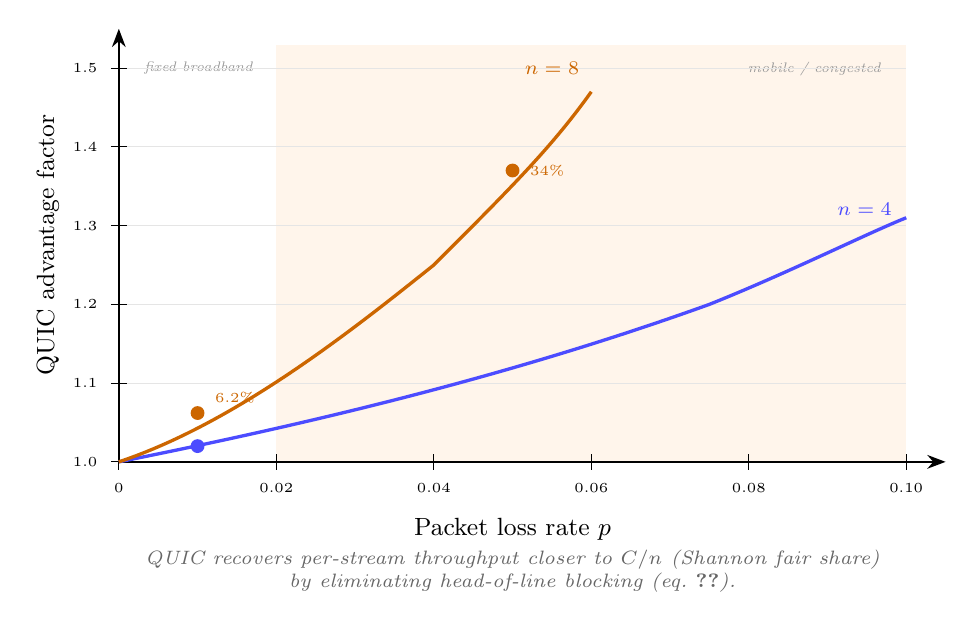
\begin{tikzpicture}[>=Stealth]

% --- Shaded region (drawn FIRST so curves appear on top) ---
\fill[orange!8] (2, 0) rectangle (10, 5.3);
\node[font=\tiny\itshape, text=black!40, anchor=north east] at (9.8, 5.2)
  {mobile / congested};
\node[font=\tiny\itshape, text=black!40, anchor=north west] at (0.2, 5.2)
  {fixed broadband};

% --- Grid lines ---
\foreach \y in {1, 2, 3, 4, 5} {
  \draw[gray!20] (0, \y) -- (10, \y);
}

% --- Axes ---
\draw[->, thick] (0, 0) -- (10.5, 0);
\draw[->, thick] (0, 0) -- (0, 5.5);

% --- Axis titles (positioned to clear tick labels) ---
\node[font=\small] at (5, -0.85) {Packet loss rate $p$};
\node[font=\small, rotate=90] at (-0.9, 2.75) {QUIC advantage factor};

% --- X-axis labels ---
\foreach \x/\lab in {0/0, 2/0.02, 4/0.04, 6/0.06, 8/0.08, 10/0.10} {
  \draw (\x, -0.1) -- (\x, 0.1);
  \node[font=\tiny, anchor=north] at (\x, -0.15) {\lab};
}

% --- Y-axis labels ---
\foreach \y/\lab in {0/1.0, 1/1.1, 2/1.2, 3/1.3, 4/1.4, 5/1.5} {
  \draw (-0.1, \y) -- (0.1, \y);
  \node[font=\tiny, anchor=east] at (-0.15, \y) {\lab};
}

% --- n=4 curve: 1/(1-p)^2 ---
\draw[very thick, blue!70]
  (0, 0) .. controls (2.5, 0.5) and (5, 1.1) ..
  (7.5, 2.0) .. controls (8.5, 2.4) and (9.5, 2.9) ..
  (10, 3.1);
\node[font=\scriptsize, blue!70, anchor=south west] at (9.0, 3.0)
  {$n = 4$};

% --- n=8 curve: 1/(1-p)^6 ---
\draw[very thick, orange!80!black]
  (0, 0) .. controls (1.5, 0.5) and (3, 1.7) ..
  (4, 2.5) .. controls (5, 3.5) and (5.5, 4.0) ..
  (6, 4.7);
\node[font=\scriptsize, orange!80!black, anchor=south] at (5.5, 4.8)
  {$n = 8$};

% --- Reference points ---
\fill[orange!80!black] (1.0, 0.62) circle (2.5pt);
\node[font=\tiny, orange!80!black, anchor=south west] at (1.1, 0.62)
  {6.2\%};

\fill[orange!80!black] (5.0, 3.7) circle (2.5pt);
\node[font=\tiny, orange!80!black, anchor=west] at (5.1, 3.7)
  {34\%};

\fill[blue!70] (1.0, 0.20) circle (2.5pt);

% --- Annotation ---
\node[font=\scriptsize\itshape, text=black!60, align=center,
  anchor=north] at (5.0, -1.0)
  {QUIC recovers per-stream throughput closer to $C/n$ (Shannon fair share)\\
   by eliminating head-of-line blocking (eq.~\ref{eq:hol-ratio}).};

\end{tikzpicture}
\caption{QUIC advantage factor $1/(1-p)^{n-2}$ over TCP for multiplexed
  streams. At 5\% loss with $n=8$ streams, QUIC delivers 34\% more
  per-stream throughput by maintaining independence at the transport layer.}
\label{fig:hol-blocking}
\end{figure}

\subsubsection{Connection Establishment Latency}

Let $\tau$ denote the one-way latency (half the round-trip time). The
information-carrying capacity during connection establishment is zero;
the handshake represents pure overhead. The time to first useful byte
is:
\begin{align}
  T_{\text{TCP+TLS\,1.3}} &= 2\tau_{\text{TCP}} + \tau_{\text{TLS}}
    = 3\tau \quad \text{(1-RTT TLS~1.3)} \label{eq:tcp-setup} \\
  T_{\text{QUIC}} &= \tau \quad \text{(1-RTT)}
    \label{eq:quic-setup} \\
  T_{\text{QUIC,\,0-RTT}} &= 0 \quad \text{(resumption)}
    \label{eq:quic-0rtt}
\end{align}
The QUIC 0-RTT case (\ref{eq:quic-0rtt}) eliminates the handshake
entirely for resumed connections. The information lost during
handshake dead time, relative to steady-state capacity, is:
\begin{equation}
  I_{\text{lost}} = C_{\text{link}} \cdot T_{\text{setup}}
  \label{eq:ilost}
\end{equation}
For a 120~Mbps link with $\tau = 25$~ms (typical fixed broadband in
2026), the TCP+TLS~1.3 handshake wastes $120 \times 10^6 \times 0.075
= 9 \times 10^6$ bits (1.125~MB), while QUIC~1-RTT wastes only
$3 \times 10^6$ bits (375~KB).

\subsection{Source Coding Efficiency}

The rate-distortion function $R(D)$ defines the minimum bit rate
required to represent a source at distortion level $D$. For a
Gaussian source with variance $\sigma^2$ under mean squared error
distortion:
\begin{equation}
  R(D) = \frac{1}{2} \log_2 \frac{\sigma^2}{D}
    \quad \text{[bits/sample]}
  \label{eq:rate-distortion}
\end{equation}

\excursus{Excursus: Why Gaussian source?}{The Gaussian memoryless model is used
because it yields the highest (worst-case) $R(D)$ among all sources of equal
variance. Any codec that approaches the Gaussian bound on real video is
therefore doing at least as well as the bound predicts --- the true $R(D)$ for
spatially and temporally correlated video lies below the Gaussian curve, making
it a conservative benchmark.}

No practical codec achieves $R(D)$;\footnote{The $R(D)$ curve in
Figure~\ref{fig:rate-distortion} is the Gaussian memoryless source bound
(equation~\ref{eq:rate-distortion}), which is an upper bound on the true
$R(D)$ for non-Gaussian sources such as video.  Additionally, $R(D)$ assumes
zero excess-distortion probability, whereas practical codecs permit a
frame-level excess-distortion probability on the order of $10^{-6}$ to
$10^{-8}$.  Both factors allow codec operating points measured on real content
to approach or marginally cross the Gaussian bound.} real codecs operate at
some rate $R_{\text{codec}} > R(D)$. We define the coding efficiency gap as:
\begin{equation}
  \Delta = \frac{R_{\text{codec}} - R(D)}{R(D)}
  \label{eq:coding-gap}
\end{equation}

The codecs in the WebRTC stack can be ordered by their empirical
proximity to $R(D)$ for typical video content at conversational
resolutions (720p, 30~fps). Using published Bj\o ntegaard Delta (BD)
rate measurements:
\begin{equation}
  R_{\text{H.264}} > R_{\text{VP9}} > R_{\text{AV1}}
    > R(D)
  \label{eq:codec-ordering}
\end{equation}

Specifically, the empirical rate savings at equivalent PSNR are
approximately:
\begin{align}
  R_{\text{VP9}}  &\approx 0.65 \cdot R_{\text{H.264}}
    \quad (\sim\!35\% \text{ savings}) \label{eq:vp9-savings} \\
  R_{\text{AV1}}  &\approx 0.70 \cdot R_{\text{VP9}}
    \approx 0.46 \cdot R_{\text{H.264}}
    \quad (\sim\!30\% \text{ over VP9})
  \label{eq:av1-savings}
\end{align}

\begin{figure}[ht]
\centering
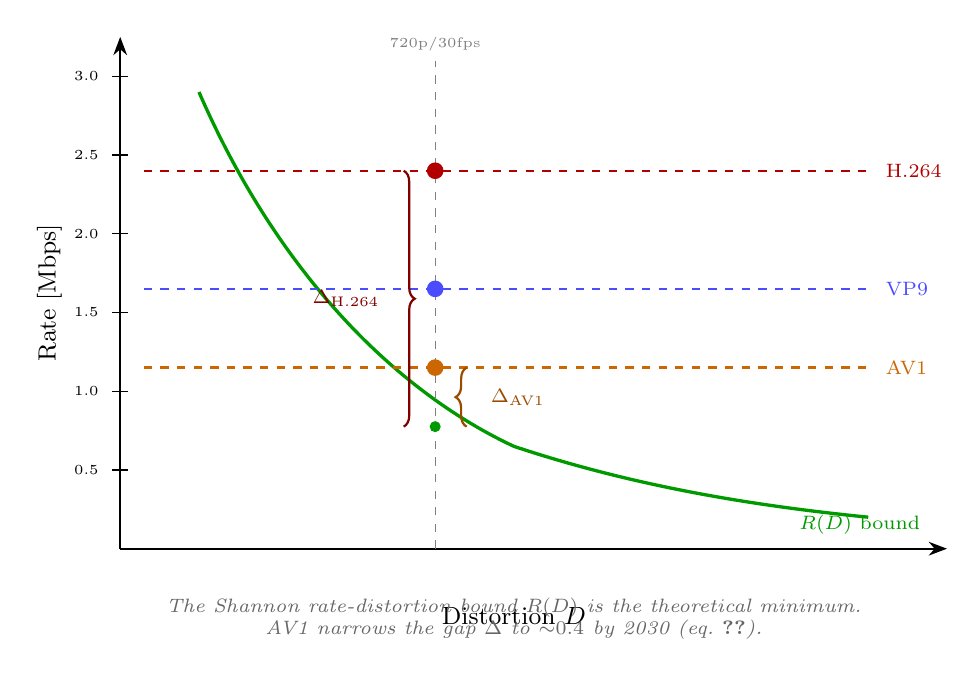
\begin{tikzpicture}[>=Stealth]

% --- Axes ---
\draw[->, thick] (0, 0) -- (10.5, 0);
\draw[->, thick] (0, 0) -- (0, 6.5);

% --- Axis titles ---
\node[font=\small] at (5, -0.85) {Distortion $D$};
\node[font=\small, rotate=90] at (-0.9, 3.25) {Rate [Mbps]};

% --- Y-axis rate labels ---
\foreach \y/\lab in {1.0/0.5, 2.0/1.0, 3.0/1.5, 4.0/2.0, 5.0/2.5, 6.0/3.0} {
  \draw (-0.1, \y) -- (0.1, \y);
  \node[font=\tiny, anchor=east] at (-0.15, \y) {\lab};
}

% --- R(D) Shannon bound curve ---
\draw[very thick, green!60!black]
  (1.0, 5.8) .. controls (2.0, 3.5) and (3.5, 2.0) ..
  (5.0, 1.3) .. controls (6.5, 0.8) and (8.0, 0.55) ..
  (9.5, 0.4);
\node[font=\scriptsize, green!60!black, anchor=north west] at (8.5, 0.55)
  {$R(D)$ bound};

% --- Reference distortion line (720p/30fps operating point) ---
\draw[thin, gray, dashed] (4.0, 0) -- (4.0, 6.2);
\node[font=\tiny, gray, anchor=south] at (4.0, 6.2) {720p/30fps};

% --- R(D) value at reference distortion ---
\fill[green!60!black] (4.0, 1.55) circle (2pt);

% --- Codec operating points at reference distortion ---
% H.264: ~2.5 Mbps
\draw[thick, dashed, red!70!black] (0.3, 4.8) -- (9.5, 4.8);
\fill[red!70!black] (4.0, 4.8) circle (3pt);
\node[font=\scriptsize, red!70!black, anchor=west] at (9.6, 4.8) {H.264};

% VP9: ~1.6 Mbps (0.65 * H.264)
\draw[thick, dashed, blue!70] (0.3, 3.3) -- (9.5, 3.3);
\fill[blue!70] (4.0, 3.3) circle (3pt);
\node[font=\scriptsize, blue!70, anchor=west] at (9.6, 3.3) {VP9};

% AV1: ~1.15 Mbps (0.46 * H.264)
\draw[thick, dashed, orange!80!black] (0.3, 2.3) -- (9.5, 2.3);
\fill[orange!80!black] (4.0, 2.3) circle (3pt);
\node[font=\scriptsize, orange!80!black, anchor=west] at (9.6, 2.3) {AV1};

% --- Gap annotations (braces) ---
% H.264 gap
\draw[decorate, decoration={brace, amplitude=4pt, mirror},
  thick, red!50!black]
  (3.6, 1.55) -- (3.6, 4.8)
  node[midway, anchor=east, font=\scriptsize, xshift=-5pt]
  {$\Delta_{\text{H.264}}$};

% AV1 gap
\draw[decorate, decoration={brace, amplitude=4pt},
  thick, orange!60!black]
  (4.4, 1.55) -- (4.4, 2.3)
  node[midway, anchor=west, font=\scriptsize, xshift=5pt]
  {$\Delta_{\text{AV1}}$};

% --- Annotation ---
\node[font=\scriptsize\itshape, text=black!60, align=center,
  anchor=north] at (5.0, -0.5)
  {The Shannon rate-distortion bound $R(D)$ is the theoretical minimum.\\
   AV1 narrows the gap $\Delta$ to ${\sim}0.4$ by 2030 (eq.~\ref{eq:coding-gap}).};

\end{tikzpicture}
\caption{Codec operating rates vs.\ the Shannon rate-distortion bound $R(D)$
  at 720p/30fps. Each codec operates above the theoretical minimum; the gap
  $\Delta$ (eq.~\ref{eq:coding-gap}) shrinks from H.264 through VP9 to AV1,
  approaching but never reaching the bound.}
\label{fig:rate-distortion}
\end{figure}

\subsubsection{Codec Entropy and WebCodecs}

The WebCodecs API (W3C Working Draft) exposes per-frame codec access,
allowing measurement and control of the instantaneous encoding rate.
For a video frame $f_t$ at time $t$, the encoder output has empirical
entropy:
\begin{equation}
  \hat{H}(f_t) = -\sum_{s \in \mathcal{S}}
    p(s \mid f_t) \log_2 p(s \mid f_t)
  \label{eq:frame-entropy}
\end{equation}
where $\mathcal{S}$ is the set of symbols emitted by the entropy coder
(CABAC for H.264/AV1, arithmetic coding for VP9). WebCodecs enables
applications to observe $|E(f_t)|$ (the encoded frame size in bits)
directly, which serves as a practical upper bound on
$\hat{H}(f_t)$:
\begin{equation}
  \hat{H}(f_t) \leq |E(f_t)| \leq R_{\text{codec}} / \text{fps}
  \label{eq:entropy-bound}
\end{equation}

\subsection{Effective Information Rate by Time Horizon}

We now combine transport and source coding measures to estimate the
effective information rate for a representative real-time video
session: a single 720p/30fps video call with one audio channel.

\excursus{Excursus: Why 720p?}{Throughout this appendix, 720p/30fps is used as
a fixed reference for cross-era comparison, not as a prediction that 720p
remains the dominant conferencing resolution. The bandwidth surplus quantified
below is precisely what enables migration to 1080p (feasible by ${\sim}$2028
with AV1 hardware encode at today's 720p bit rates) and 4K (feasible by
${\sim}$2030). The 720p baseline makes the efficiency gains legible: the same
task gets cheaper, freeing capacity for higher quality or more streams.}

Define the \emph{net information rate} as:
\begin{equation}
  I_{\text{net}} = R_{\text{codec}} \cdot \eta_{\text{transport}}
    \cdot (1 - \rho_{\text{overhead}})
    \cdot (1 - p_{\text{loss}})
  \label{eq:inet}
\end{equation}

\begin{table}[ht]
\centering
\small
\renewcommand{\arraystretch}{1.4}
\begin{tabularx}{\textwidth}{lXXX}
\toprule
\textbf{Parameter} & \textbf{March 2026} & \textbf{2027--2028} &
  \textbf{2029--2031} \\
\midrule
Median link capacity &
  120~Mbps &
  $\sim$150~Mbps &
  200--300~Mbps \\
Dominant codec (WebRTC) &
  VP9 / H.264 &
  VP9 / AV1 (HW) &
  AV1 (HW default) \\
Codec rate (720p/30fps) &
  1.5--2.5~Mbps &
  1.0--1.8~Mbps &
  0.7--1.2~Mbps \\
$\eta_{\text{transport}}$ &
  0.92 (QUIC) &
  0.93 &
  0.94 \\
$\rho_{\text{overhead}}$ (SRTP+QUIC) &
  0.06 &
  0.05 &
  0.04 \\
Typical loss $p$ &
  0.01--0.03 &
  0.01--0.02 &
  0.005--0.01 \\
$I_{\text{net}}$ (720p video) &
  1.3--2.2~Mbps &
  0.9--1.6~Mbps &
  0.6--1.1~Mbps \\
$I_{\text{net}}$ as \% of $C_{\text{link}}$ &
  1.1--1.8\% &
  0.6--1.1\% &
  0.2--0.6\% \\
\bottomrule
\end{tabularx}
\caption{Effective information rate for a 720p/30fps WebRTC video stream.
  The declining ratio $I_{\text{net}} / C_{\text{link}}$ reflects both
  improved codec efficiency and growing link capacity, freeing bandwidth
  for higher resolutions, additional streams, or concurrent data
  channels.}
\label{tab:inet}
\end{table}

The declining ratio $I_{\text{net}} / C_{\text{link}}$ in
Table~\ref{tab:inet} is the central quantitative observation: by 2030, a
720p video call consumes less than 0.5\% of available link capacity. The
surplus capacity enables qualitative changes --- 4K video conferencing,
multi-stream layouts, or concurrent data channels via WebTransport ---
that are quantitatively infeasible in 2026.

\begin{figure}[ht]
\centering
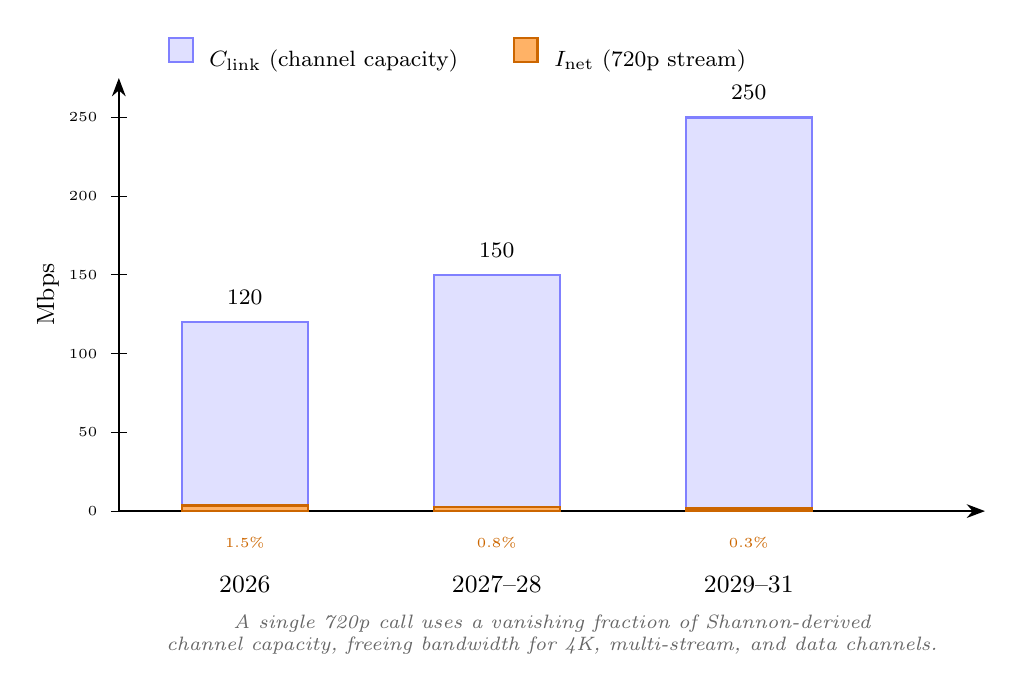
\begin{tikzpicture}[>=Stealth]

% --- Axes ---
\draw[->, thick] (0, 0) -- (11, 0);
\draw[->, thick] (0, 0) -- (0, 5.5);

% --- Axis title ---
\node[font=\small, rotate=90] at (-0.9, 2.75) {Mbps};

% --- Y-axis labels ---
\foreach \y/\lab in {0/0, 1/50, 2/100, 3/150, 4/200, 5/250} {
  \draw (-0.1, \y) -- (0.1, \y);
  \node[font=\tiny, anchor=east] at (-0.15, \y) {\lab};
}

% --- Group: March 2026 ---
% C_link = 120 Mbps -> y = 2.4
\fill[blue!12] (0.8, 0) rectangle (2.4, 2.4);
\draw[blue!50, thick] (0.8, 0) rectangle (2.4, 2.4);
% I_net = 1.75 Mbps (midpoint) -> y = 0.035
\fill[orange!60] (0.8, 0) rectangle (2.4, 0.07);
\draw[orange!80!black, thick] (0.8, 0) rectangle (2.4, 0.07);
\node[font=\footnotesize, anchor=south] at (1.6, 2.5) {120};
\node[font=\tiny, orange!80!black] at (1.6, -0.4) {1.5\%};
\node[font=\small, anchor=north] at (1.6, -0.7) {2026};

% --- Group: 2027--2028 ---
% C_link = 150 Mbps -> y = 3.0
\fill[blue!12] (4.0, 0) rectangle (5.6, 3.0);
\draw[blue!50, thick] (4.0, 0) rectangle (5.6, 3.0);
% I_net = 1.25 Mbps (midpoint) -> y = 0.025
\fill[orange!60] (4.0, 0) rectangle (5.6, 0.05);
\draw[orange!80!black, thick] (4.0, 0) rectangle (5.6, 0.05);
\node[font=\footnotesize, anchor=south] at (4.8, 3.1) {150};
\node[font=\tiny, orange!80!black] at (4.8, -0.4) {0.8\%};
\node[font=\small, anchor=north] at (4.8, -0.7) {2027--28};

% --- Group: 2029--2031 ---
% C_link = 250 Mbps -> y = 5.0
\fill[blue!12] (7.2, 0) rectangle (8.8, 5.0);
\draw[blue!50, thick] (7.2, 0) rectangle (8.8, 5.0);
% I_net = 0.85 Mbps (midpoint) -> y = 0.017
\fill[orange!60] (7.2, 0) rectangle (8.8, 0.034);
\draw[orange!80!black, thick] (7.2, 0) rectangle (8.8, 0.034);
\node[font=\footnotesize, anchor=south] at (8.0, 5.1) {250};
\node[font=\tiny, orange!80!black] at (8.0, -0.4) {0.3\%};
\node[font=\small, anchor=north] at (8.0, -0.7) {2029--31};

% --- Legend ---
\node[anchor=west, font=\footnotesize] at (0.5, 5.8) {%
  \tikz[baseline=-0.5ex]{\fill[blue!12] (0,0) rectangle (0.3,0.3);
    \draw[blue!50, thick] (0,0) rectangle (0.3,0.3);}
  ~$C_{\text{link}}$ (channel capacity) \qquad
  \tikz[baseline=-0.5ex]{\fill[orange!60] (0,0) rectangle (0.3,0.3);
    \draw[orange!80!black, thick] (0,0) rectangle (0.3,0.3);}
  ~$I_{\text{net}}$ (720p stream)};

% --- Annotation ---
\node[font=\scriptsize\itshape, text=black!60, align=center,
  anchor=north] at (5.5, -1.2)
  {A single 720p call uses a vanishing fraction of Shannon-derived\\
   channel capacity, freeing bandwidth for 4K, multi-stream, and data channels.};

\end{tikzpicture}
\caption{Channel capacity $C_{\text{link}}$ vs.\ effective information rate
  $I_{\text{net}}$ for a single 720p/30fps stream across time horizons. The
  orange bar (stream rate) is barely visible against the blue bar (capacity),
  illustrating the growing surplus as codecs improve and bandwidth increases.}
\label{fig:inet-capacity}
\end{figure}

\subsection{Security Entropy and Key Space}

The DTLS-SRTP security architecture (RFCs~8827, 3711) protects all
WebRTC media. Information-theoretic security requires that the key
entropy exceed the information content of the protected material.

For a DTLS~1.3 handshake with ECDHE on P-256, the key agreement
provides:
\begin{equation}
  H_{\text{key}} = 128 \text{~bits of security}
  \label{eq:key-entropy}
\end{equation}

The SRTP master key is 128 bits (AES-128-GCM), giving an exhaustive
search cost of $2^{128}$ operations. The total information content of a
one-hour 720p video call at 2~Mbps is:
\begin{equation}
  I_{\text{call}} = 2 \times 10^6 \times 3600
    = 7.2 \times 10^9 \text{~bits}
    \approx 2^{32.7} \text{~bits}
  \label{eq:call-content}
\end{equation}

The ratio of key entropy to protected content:
\begin{equation}
  \frac{H_{\text{key}}}{I_{\text{call}}}
    = \frac{128}{32.7} \approx 3.91
  \label{eq:security-margin}
\end{equation}

This ratio remains comfortably above~1 even for much longer sessions.
For a continuous 24-hour 4K AV1 stream at 15~Mbps:
\begin{equation}
  I_{\text{stream}} = 15 \times 10^6 \times 86400
    = 1.296 \times 10^{12} \text{~bits}
    \approx 2^{40.2} \text{~bits}
\end{equation}
yielding $H_{\text{key}} / I_{\text{stream}} \approx 3.18$, still
well above the threshold.

\subsubsection{End-to-End Encryption via Encoded Transforms}

The RTCRtpScriptTransform API (Encoded Transforms) enables
application-layer E2EE within the WebRTC pipeline. From an
information-theoretic perspective, this introduces a second encryption
layer with its own key, creating a \emph{nested channel}:
\begin{equation}
  X \xrightarrow{\;K_{\text{E2EE}}\;}
  E_1(X) \xrightarrow{\;K_{\text{SRTP}}\;}
  E_2(E_1(X))
  \label{eq:nested}
\end{equation}

The mutual information between the ciphertext and plaintext, given
neither key, satisfies:
\begin{equation}
  I\!\left(X;\, E_2(E_1(X))\right) \leq
    \min\!\big(H(K_{\text{E2EE}})^{-1},\;
    H(K_{\text{SRTP}})^{-1}\big)
    \cdot I_{\text{call}}
  \label{eq:mutual-e2ee}
\end{equation}

In practice, with $H(K_{\text{E2EE}}) = H(K_{\text{SRTP}}) = 128$
bits, this quantity is negligible ($\ll 1$ bit for any practical
session length), confirming that the nested encryption provides
information-theoretic confidentiality well beyond computational
security guarantees.

Today (March~2026), Encoded Transforms remain Chrome-only. By
2027--2028 (Section~8.3), cross-browser standardization will make
this nested channel universally available. By 2029--2031, SFrame
for group calls will extend this to $n$-party sessions, where the
mutual information between any non-member and the group plaintext
remains negligible:
\begin{equation}
  I\!\left(X;\, E(X) \;\middle|\; K_i \notin
    \{K_1, \ldots, K_n\}\right) \approx 0
  \label{eq:sframe}
\end{equation}

\subsection{WebTransport: Unreliable Datagrams and Channel Capacity}

WebTransport (RFC~9297) introduces unreliable datagrams to browser-server
communication. For latency-sensitive applications (game state, sensor
telemetry), the relevant measure is not throughput but
\emph{freshness-weighted information rate}. Define the value of a
datagram as exponentially decaying with delivery latency $\delta$:
\begin{equation}
  V(\delta) = e^{-\lambda \delta}
  \label{eq:freshness}
\end{equation}
where $\lambda > 0$ is an application-specific decay rate. The
effective information rate under unreliable delivery is:
\begin{equation}
  I_{\text{WT}} = R_{\text{send}} \cdot (1 - p_{\text{loss}})
    \cdot \mathbb{E}\!\left[e^{-\lambda \delta}\right]
  \label{eq:iwt}
\end{equation}

Under reliable delivery (TCP/WebSocket), a retransmission delays
subsequent data, so:
\begin{equation}
  I_{\text{WS}} = R_{\text{send}}
    \cdot \mathbb{E}\!\left[e^{-\lambda(\delta + p \cdot 2\tau)}\right]
  \label{eq:iws}
\end{equation}

The ratio $I_{\text{WT}} / I_{\text{WS}}$ exceeds 1 when:
\begin{equation}
  (1 - p) \cdot e^{\lambda \cdot p \cdot 2\tau} > 1
  \quad \Longleftrightarrow \quad
  \lambda > \frac{-\ln(1 - p)}{2 p \tau}
  \label{eq:wt-advantage}
\end{equation}

For $p = 0.02$ and $\tau = 25$~ms, this gives $\lambda > 20.2$~s$^{-1}$
(half-life $< 34$~ms).

\excursus{Excursus: Why $p = 0.02$ and $\tau = 25$\,ms?}{These values represent
median fixed-broadband conditions in 2026 (Table~\ref{tab:inet}). On mobile or
congested links ($p \approx 0.05$, $\tau \approx 50$\,ms), the threshold
$\lambda^*$ drops to ${\sim}10$\,s$^{-1}$, broadening WebTransport's advantage
to applications with data half-lives up to ${\sim}70$\,ms. The fixed-broadband
reference is thus conservative: mobile scenarios favor unreliable delivery even
more strongly.}

Any application where data older than
$\sim$30~ms is useless benefits from WebTransport's unreliable
mode over WebSocket --- precisely the regime of interactive gaming, live
cursor tracking, and real-time sensor feeds.

As of March~2026, Safari does not support WebTransport
(Section~5), limiting coverage to $\sim$82\%. By 2027--2028
(Section~8.2), universal support will allow applications to rely on
(\ref{eq:iwt}) without fallback paths.

\begin{figure}[ht]
\centering
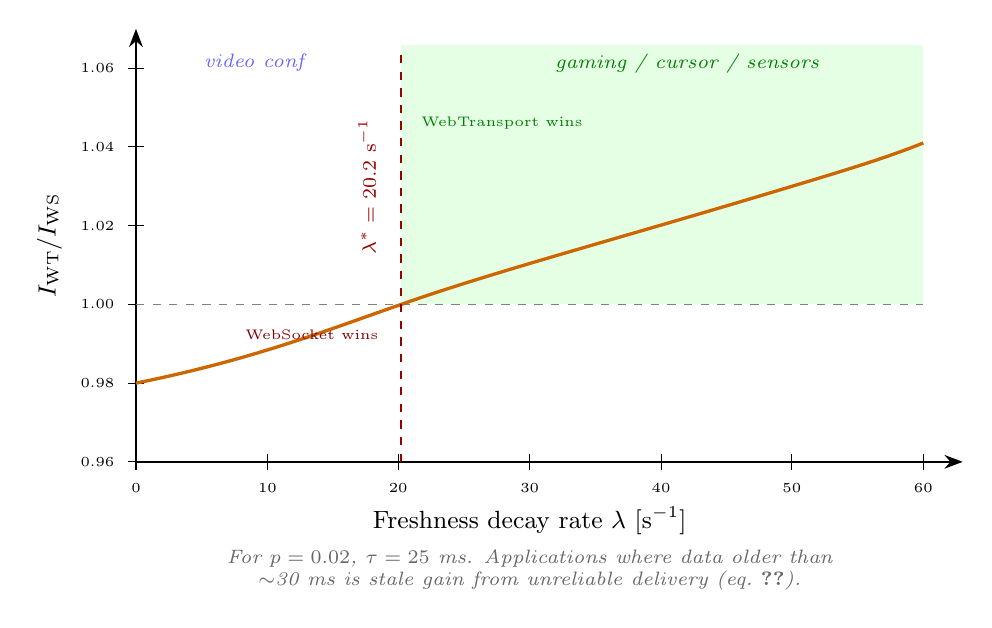
\begin{tikzpicture}[>=Stealth]

% --- Axes ---
\draw[->, thick] (0, 0) -- (10.5, 0);
\draw[->, thick] (0, 0) -- (0, 5.5);

% --- Axis titles (positioned to clear tick labels) ---
\node[font=\small] at (5, -0.75)
  {Freshness decay rate $\lambda$ [s$^{-1}$]};
\node[font=\small, rotate=90] at (-1.1, 2.75)
  {$I_{\text{WT}} / I_{\text{WS}}$};

% --- X-axis labels ---
\foreach \x/\lab in {0/0, 1.67/10, 3.33/20, 5.0/30, 6.67/40, 8.33/50, 10/60} {
  \draw (\x, -0.1) -- (\x, 0.1);
  \node[font=\tiny, anchor=north] at (\x, -0.15) {\lab};
}

% --- Y-axis labels (0.96 to 1.06, each 0.02 = 1 unit) ---
\foreach \y/\lab in {0/0.96, 1/0.98, 2/1.00, 3/1.02, 4/1.04, 5/1.06} {
  \draw (-0.1, \y) -- (0.1, \y);
  \node[font=\tiny, anchor=east] at (-0.15, \y) {\lab};
}

% --- Ratio = 1.0 line (y=2 maps to ratio 1.0) ---
\draw[thin, gray, dashed] (0, 2) -- (10, 2);

% --- Shade WebTransport advantage region ---
% lambda* = 20.2 -> x = 3.37
\fill[green!10] (3.37, 2) rectangle (10, 5.3);

% --- I_WT/I_WS curve: 0.98*exp(lambda*0.001) ---
% Y range: 0.96-1.06 (each 0.02 = 1 unit). lambda=0: y=1, lambda*=20.2: y=2, lambda=60: y=4.05
\draw[very thick, orange!80!black]
  (0, 1.0) .. controls (1.5, 1.3) and (2.5, 1.7) ..
  (3.37, 2.0) .. controls (4.5, 2.4) and (6, 2.8) ..
  (8, 3.4) .. controls (9, 3.7) and (9.5, 3.85) ..
  (10, 4.05);

% --- Threshold line ---
\draw[thick, dashed, red!60!black] (3.37, 0) -- (3.37, 5.2);
\node[font=\scriptsize, red!60!black, anchor=south, rotate=90] at (3.17, 3.5)
  {$\lambda^* = 20.2$ s$^{-1}$};

% --- Application regime labels ---
\node[font=\scriptsize\itshape, text=blue!60, anchor=north] at (1.5, 5.3)
  {video conf};
\node[font=\scriptsize\itshape, text=green!50!black, anchor=north] at (7.0, 5.3)
  {gaming / cursor / sensors};

% --- Mark advantage/disadvantage ---
\node[font=\tiny, text=red!50!black, anchor=north east] at (3.2, 1.8)
  {WebSocket wins};
\node[font=\tiny, text=green!50!black, anchor=north west] at (3.5, 4.5)
  {WebTransport wins};

% --- Annotation ---
\node[font=\scriptsize\itshape, text=black!60, align=center,
  anchor=north] at (5.0, -1.0)
  {For $p = 0.02$, $\tau = 25$~ms. Applications where data older than\\
   ${\sim}$30~ms is stale gain from unreliable delivery (eq.~\ref{eq:wt-advantage}).};

\end{tikzpicture}
\caption{Freshness-weighted information rate ratio $I_{\text{WT}} / I_{\text{WS}}$
  as a function of decay rate $\lambda$. Above the threshold $\lambda^*$,
  WebTransport's unreliable datagrams deliver more useful information per
  unit time than WebSocket's reliable delivery, because retransmission
  wastes capacity on stale data.}
\label{fig:freshness}
\end{figure}

\subsection{Projections Summary and Practical Implications}

\begin{table}[ht]
\centering
\small
\renewcommand{\arraystretch}{1.4}
\begin{tabularx}{\textwidth}{lXXX}
\toprule
\textbf{Measure} & \textbf{March 2026} & \textbf{2027--2028} &
  \textbf{2029--2031} \\
\midrule
Channel capacity $C_{\text{link}}$ &
  120~Mbps &
  150~Mbps &
  250~Mbps \\
HOL blocking factor $(1\!-\!p)^{n-2}$ at $n\!=\!8$ &
  0.94 ($p\!=\!0.01$) &
  0.94 &
  0.97 ($p\!=\!0.005$) \\
Source coding gap $\Delta$ &
  VP9: $\sim$0.8 &
  AV1 HW: $\sim$0.5 &
  AV1 opt: $\sim$0.4 \\
$I_{\text{net}}$ per 720p stream &
  1.3--2.2~Mbps &
  0.9--1.6~Mbps &
  0.6--1.1~Mbps \\
Max 720p streams in $C_{\text{link}}$ &
  $\sim$55--90 &
  $\sim$95--165 &
  $\sim$230--415 \\
E2EE availability &
  Chrome only &
  Cross-browser &
  SFrame $n$-party \\
WebTransport coverage &
  82\% &
  $\sim$100\% &
  100\% \\
Freshness threshold $\lambda^*$ &
  20.2~s$^{-1}$ &
  $\sim$18~s$^{-1}$ &
  $\sim$15~s$^{-1}$ \\
\bottomrule
\end{tabularx}
\caption{Information-theoretic measures across time horizons. $\Delta$
  is the coding efficiency gap (\ref{eq:coding-gap}), $I_{\text{net}}$
  is the net information rate (\ref{eq:inet}), and $\lambda^*$ is the
  freshness decay threshold above which WebTransport dominates WebSocket
  (\ref{eq:wt-advantage}).}
\label{tab:projections}
\end{table}

The trajectory is clear: the combination of improving source coding
(AV1 hardware), expanding channel capacity (broadband growth), and
maturing transport protocols (QUIC universal, WebTransport universal)
drives the \emph{information cost per unit of communicated experience}
steadily downward. The remaining question is not whether the
Shannon capacity suffices --- it already does, by orders of magnitude
--- but how efficiently the protocol stack converts that capacity into
delivered, fresh, secure information at the application layer. By
2030, the gap between theoretical capacity and realized throughput will
be the narrowest it has ever been for browser-based real-time
communication.

\subsubsection{What the Theory Means for Applications}

The equations and figures in this appendix are not purely academic. Each
theoretical result maps to a concrete design decision that application
developers face today and over the next five years.

\textbf{Codec selection determines bandwidth cost, not quality.}
The rate-distortion analysis (Section~A.2, Figure~\ref{fig:rate-distortion})
shows that AV1 operates at roughly 46\% of H.264's bit rate for equivalent
perceptual quality at 720p. In practice, this means a WebRTC application
switching from H.264 to AV1 can either halve its bandwidth consumption at
the same quality or substantially increase resolution (e.g., 720p to 1080p)
within the same bandwidth envelope. By 2030, with AV1 hardware encoding
ubiquitous and the coding gap $\Delta$ approaching 0.4, further codec
improvements yield diminishing returns --- the stack will be operating close
enough to the Shannon rate-distortion bound that the next generation of
efficiency gains will come from transport and architecture, not codecs alone.

\textbf{QUIC's advantage is situational but decisive on bad networks.}
The head-of-line blocking analysis (Section~A.1.1,
Figure~\ref{fig:hol-blocking}) shows that QUIC's per-stream throughput
advantage over TCP is modest on good networks (6\% at 1\% loss) but
substantial on degraded ones (34\% at 5\% loss). The practical implication
is that applications targeting mobile users, emerging markets, or congested
enterprise networks --- precisely the environments where real-time
communication is hardest --- benefit disproportionately from QUIC-based
transports. For a video conference with 8 participants on a cellular
connection experiencing 3--5\% packet loss, the difference between QUIC and
TCP is the difference between usable and degraded video.

\textbf{Connection latency is a solved problem for returning users.}
The handshake analysis (Section~A.1.2) shows that QUIC 0-RTT eliminates
connection establishment overhead entirely for resumed connections. For a
WebTransport application that a user opens daily --- a collaboration tool,
a live dashboard, a recurring meeting client --- the time to first useful
byte drops to zero. The 1.125~MB of wasted capacity during a TCP+TLS
handshake on a 120~Mbps link may seem small, but for latency-sensitive
applications where the first 100~ms of perceived responsiveness determines
user experience, the difference is measurable.

\textbf{Bandwidth surplus enables architectural ambition.}
The effective information rate analysis (Section~A.3,
Figure~\ref{fig:inet-capacity}) reveals the most consequential practical
finding: a single 720p video stream consumes a vanishing fraction of
available link capacity (under 0.5\% by 2030). This surplus is not merely
``headroom'' --- it is the resource that makes new application architectures
feasible. A 250~Mbps link can theoretically carry 230--415 simultaneous 720p
streams. In practice, this means applications can afford to run multiple
concurrent media flows (video, screen share, spatial audio), data channels
(collaborative editing, file transfer), and telemetry streams without
contending for bandwidth. The constraint shifts from ``can the network carry
this?''\ to ``can the application manage this complexity?''

\textbf{End-to-end encryption adds negligible overhead.}
The security analysis (Section~A.4) confirms that the nested DTLS-SRTP plus
E2EE architecture imposes no meaningful information-theoretic cost. The key
entropy ($2^{128}$) exceeds the information content of any practical session
by a factor of at least 3. For application developers, this means E2EE can
be treated as a default rather than a premium feature --- there is no
bandwidth, latency, or capacity penalty for encrypting at the application
layer on top of the transport-layer encryption that WebRTC already mandates.
The only constraint is API availability, which moves from Chrome-only (2026)
to universal (2028).

\textbf{WebTransport unlocks real-time data that WebSocket cannot serve.}
The freshness analysis (Section~A.5, Figure~\ref{fig:freshness}) quantifies
when unreliable delivery outperforms reliable delivery: any data with a
useful half-life below approximately 34~ms benefits from WebTransport's
unreliable datagrams. This covers a wide class of interactive applications
--- game state synchronization, live cursor and pointer sharing, real-time
sensor feeds, collaborative whiteboard strokes --- where retransmitting a
stale update is worse than dropping it. Before WebTransport, these
applications had to choose between WebSocket (reliable but stale under loss)
and WebRTC DataChannel (unreliable mode available but requiring the full
peer-to-peer ICE/DTLS machinery). WebTransport provides the unreliable
mode with a simple client-server model over HTTP/3, removing the
architectural overhead.

\textbf{The overall picture: the stack converges on efficiency.}
Taken together, the information-theoretic measures trace a consistent
trajectory. The protocol stack is converging toward the theoretical limits
established by Shannon: codecs approach the rate-distortion bound, transports
eliminate unnecessary blocking and handshake overhead, and encryption adds
negligible cost. By 2030, the practical distance between what the standards
deliver and what information theory permits will be the smallest it has ever
been for browser-based real-time communication. The consequence for
application developers is that the infrastructure --- standards, hardware,
and networks --- will no longer be the binding constraint. The remaining
challenge is purely architectural: how to compose these efficient, universal
primitives into applications that fully exploit the capacity and low latency
they provide.

% appendix-video-compression.tex
% Standalone appendix — include from retrospective.tex via:
%   \appendix
%   % appendix-info-theory.tex
% Standalone appendix — include from retrospective.tex via:
%   \appendix
%   % appendix-info-theory.tex
% Standalone appendix — include from retrospective.tex via:
%   \appendix
%   \input{appendix-info-theory}
%
% Requires in the preamble: amsmath, amssymb, tabularx, booktabs

\section{Information-Theoretic View}
\label{app:info-theory}

This appendix applies information-theoretic measures to the real-time
web communication stack described in this document. We quantify channel
capacity, source coding efficiency, and effective information rates
across three time horizons: today (March~2026), the near term
(2027--2028), and the medium term (2029--2031). The analysis draws on
the standards, codec parameters, and infrastructure projections
developed in the main text.

\subsection{Channel Capacity of the Transport Layer}

The Shannon-Hartley theorem gives the theoretical maximum information
rate for a channel with additive white Gaussian noise:
\begin{equation}
  C = B \log_2\!\left(1 + \frac{S}{N}\right) \quad \text{[bits/s]}
  \label{eq:shannon}
\end{equation}
where $B$ is the channel bandwidth in Hz and $S/N$ is the
signal-to-noise ratio.

While the physical-layer capacity of a broadband link is governed by
(\ref{eq:shannon}), the \emph{effective} capacity available to the
application is reduced by protocol overhead, congestion control, and
transport inefficiencies. We define the effective application-layer
throughput as:
\begin{equation}
  R_{\text{eff}} = C_{\text{link}} \cdot \eta_{\text{transport}}
    \cdot (1 - \rho_{\text{overhead}})
  \label{eq:reff}
\end{equation}
where $C_{\text{link}}$ is the link-layer capacity,
$\eta_{\text{transport}} \in (0,1]$ is the transport efficiency factor
(capturing congestion control, retransmission, and multiplexing
behavior), and $\rho_{\text{overhead}} \in [0,1)$ is the fractional
protocol overhead (headers, encryption, framing).

\subsubsection{Head-of-Line Blocking and Multiplexed Capacity}

Consider $n$ independent streams multiplexed over a single connection.
Under TCP (HTTP/2), a single lost packet blocks all $n$ streams. The
expected throughput per stream under loss rate $p$ is bounded by:
\begin{equation}
  R_{\text{TCP}}^{(i)} \leq \frac{R_{\text{eff}}}{n}
    \cdot (1 - p)^{n-1}
  \label{eq:hol-tcp}
\end{equation}
because a loss in \emph{any} of the $n$ streams stalls all others. Under
QUIC (RFC~9000), streams are independent at the transport layer, so:
\begin{equation}
  R_{\text{QUIC}}^{(i)} \leq \frac{R_{\text{eff}}}{n}
    \cdot (1 - p)
  \label{eq:hol-quic}
\end{equation}
The ratio of effective per-stream throughput is:
\begin{equation}
  \frac{R_{\text{QUIC}}^{(i)}}{R_{\text{TCP}}^{(i)}}
    = \frac{1}{(1-p)^{n-2}}
  \label{eq:hol-ratio}
\end{equation}
\excursus{Excursus: Why $n = 8$?}{In a typical multi-participant video
conference, each peer contributes multiple concurrent streams: a camera video
track, an audio track, and often a screen-share or data channel. A four-person
call with two media tracks each produces $n = 8$ multiplexed streams over a
single connection --- the reference value used throughout this section. Larger
meetings (e.g.\ 10 participants with simulcast layers) push $n$ higher,
amplifying the HOL blocking effect further.}

For $n = 8$ streams (a typical multi-track video conference) at
$p = 0.01$ (1\% loss), this gives a QUIC advantage factor of
$1/(0.99)^6 \approx 1.062$, a modest 6.2\% improvement. At $p = 0.05$
(5\% loss, common on mobile or congested links), the factor is
$1/(0.95)^6 \approx 1.34$, a 34\% throughput advantage per stream.

\begin{figure}[ht]
\centering
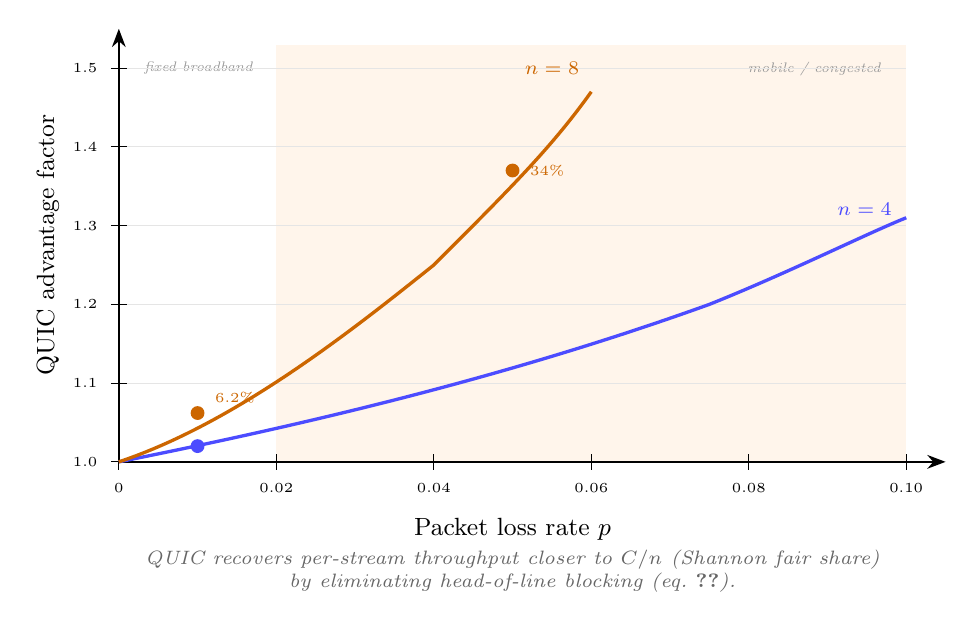
\begin{tikzpicture}[>=Stealth]

% --- Shaded region (drawn FIRST so curves appear on top) ---
\fill[orange!8] (2, 0) rectangle (10, 5.3);
\node[font=\tiny\itshape, text=black!40, anchor=north east] at (9.8, 5.2)
  {mobile / congested};
\node[font=\tiny\itshape, text=black!40, anchor=north west] at (0.2, 5.2)
  {fixed broadband};

% --- Grid lines ---
\foreach \y in {1, 2, 3, 4, 5} {
  \draw[gray!20] (0, \y) -- (10, \y);
}

% --- Axes ---
\draw[->, thick] (0, 0) -- (10.5, 0);
\draw[->, thick] (0, 0) -- (0, 5.5);

% --- Axis titles (positioned to clear tick labels) ---
\node[font=\small] at (5, -0.85) {Packet loss rate $p$};
\node[font=\small, rotate=90] at (-0.9, 2.75) {QUIC advantage factor};

% --- X-axis labels ---
\foreach \x/\lab in {0/0, 2/0.02, 4/0.04, 6/0.06, 8/0.08, 10/0.10} {
  \draw (\x, -0.1) -- (\x, 0.1);
  \node[font=\tiny, anchor=north] at (\x, -0.15) {\lab};
}

% --- Y-axis labels ---
\foreach \y/\lab in {0/1.0, 1/1.1, 2/1.2, 3/1.3, 4/1.4, 5/1.5} {
  \draw (-0.1, \y) -- (0.1, \y);
  \node[font=\tiny, anchor=east] at (-0.15, \y) {\lab};
}

% --- n=4 curve: 1/(1-p)^2 ---
\draw[very thick, blue!70]
  (0, 0) .. controls (2.5, 0.5) and (5, 1.1) ..
  (7.5, 2.0) .. controls (8.5, 2.4) and (9.5, 2.9) ..
  (10, 3.1);
\node[font=\scriptsize, blue!70, anchor=south west] at (9.0, 3.0)
  {$n = 4$};

% --- n=8 curve: 1/(1-p)^6 ---
\draw[very thick, orange!80!black]
  (0, 0) .. controls (1.5, 0.5) and (3, 1.7) ..
  (4, 2.5) .. controls (5, 3.5) and (5.5, 4.0) ..
  (6, 4.7);
\node[font=\scriptsize, orange!80!black, anchor=south] at (5.5, 4.8)
  {$n = 8$};

% --- Reference points ---
\fill[orange!80!black] (1.0, 0.62) circle (2.5pt);
\node[font=\tiny, orange!80!black, anchor=south west] at (1.1, 0.62)
  {6.2\%};

\fill[orange!80!black] (5.0, 3.7) circle (2.5pt);
\node[font=\tiny, orange!80!black, anchor=west] at (5.1, 3.7)
  {34\%};

\fill[blue!70] (1.0, 0.20) circle (2.5pt);

% --- Annotation ---
\node[font=\scriptsize\itshape, text=black!60, align=center,
  anchor=north] at (5.0, -1.0)
  {QUIC recovers per-stream throughput closer to $C/n$ (Shannon fair share)\\
   by eliminating head-of-line blocking (eq.~\ref{eq:hol-ratio}).};

\end{tikzpicture}
\caption{QUIC advantage factor $1/(1-p)^{n-2}$ over TCP for multiplexed
  streams. At 5\% loss with $n=8$ streams, QUIC delivers 34\% more
  per-stream throughput by maintaining independence at the transport layer.}
\label{fig:hol-blocking}
\end{figure}

\subsubsection{Connection Establishment Latency}

Let $\tau$ denote the one-way latency (half the round-trip time). The
information-carrying capacity during connection establishment is zero;
the handshake represents pure overhead. The time to first useful byte
is:
\begin{align}
  T_{\text{TCP+TLS\,1.3}} &= 2\tau_{\text{TCP}} + \tau_{\text{TLS}}
    = 3\tau \quad \text{(1-RTT TLS~1.3)} \label{eq:tcp-setup} \\
  T_{\text{QUIC}} &= \tau \quad \text{(1-RTT)}
    \label{eq:quic-setup} \\
  T_{\text{QUIC,\,0-RTT}} &= 0 \quad \text{(resumption)}
    \label{eq:quic-0rtt}
\end{align}
The QUIC 0-RTT case (\ref{eq:quic-0rtt}) eliminates the handshake
entirely for resumed connections. The information lost during
handshake dead time, relative to steady-state capacity, is:
\begin{equation}
  I_{\text{lost}} = C_{\text{link}} \cdot T_{\text{setup}}
  \label{eq:ilost}
\end{equation}
For a 120~Mbps link with $\tau = 25$~ms (typical fixed broadband in
2026), the TCP+TLS~1.3 handshake wastes $120 \times 10^6 \times 0.075
= 9 \times 10^6$ bits (1.125~MB), while QUIC~1-RTT wastes only
$3 \times 10^6$ bits (375~KB).

\subsection{Source Coding Efficiency}

The rate-distortion function $R(D)$ defines the minimum bit rate
required to represent a source at distortion level $D$. For a
Gaussian source with variance $\sigma^2$ under mean squared error
distortion:
\begin{equation}
  R(D) = \frac{1}{2} \log_2 \frac{\sigma^2}{D}
    \quad \text{[bits/sample]}
  \label{eq:rate-distortion}
\end{equation}

\excursus{Excursus: Why Gaussian source?}{The Gaussian memoryless model is used
because it yields the highest (worst-case) $R(D)$ among all sources of equal
variance. Any codec that approaches the Gaussian bound on real video is
therefore doing at least as well as the bound predicts --- the true $R(D)$ for
spatially and temporally correlated video lies below the Gaussian curve, making
it a conservative benchmark.}

No practical codec achieves $R(D)$;\footnote{The $R(D)$ curve in
Figure~\ref{fig:rate-distortion} is the Gaussian memoryless source bound
(equation~\ref{eq:rate-distortion}), which is an upper bound on the true
$R(D)$ for non-Gaussian sources such as video.  Additionally, $R(D)$ assumes
zero excess-distortion probability, whereas practical codecs permit a
frame-level excess-distortion probability on the order of $10^{-6}$ to
$10^{-8}$.  Both factors allow codec operating points measured on real content
to approach or marginally cross the Gaussian bound.} real codecs operate at
some rate $R_{\text{codec}} > R(D)$. We define the coding efficiency gap as:
\begin{equation}
  \Delta = \frac{R_{\text{codec}} - R(D)}{R(D)}
  \label{eq:coding-gap}
\end{equation}

The codecs in the WebRTC stack can be ordered by their empirical
proximity to $R(D)$ for typical video content at conversational
resolutions (720p, 30~fps). Using published Bj\o ntegaard Delta (BD)
rate measurements:
\begin{equation}
  R_{\text{H.264}} > R_{\text{VP9}} > R_{\text{AV1}}
    > R(D)
  \label{eq:codec-ordering}
\end{equation}

Specifically, the empirical rate savings at equivalent PSNR are
approximately:
\begin{align}
  R_{\text{VP9}}  &\approx 0.65 \cdot R_{\text{H.264}}
    \quad (\sim\!35\% \text{ savings}) \label{eq:vp9-savings} \\
  R_{\text{AV1}}  &\approx 0.70 \cdot R_{\text{VP9}}
    \approx 0.46 \cdot R_{\text{H.264}}
    \quad (\sim\!30\% \text{ over VP9})
  \label{eq:av1-savings}
\end{align}

\begin{figure}[ht]
\centering
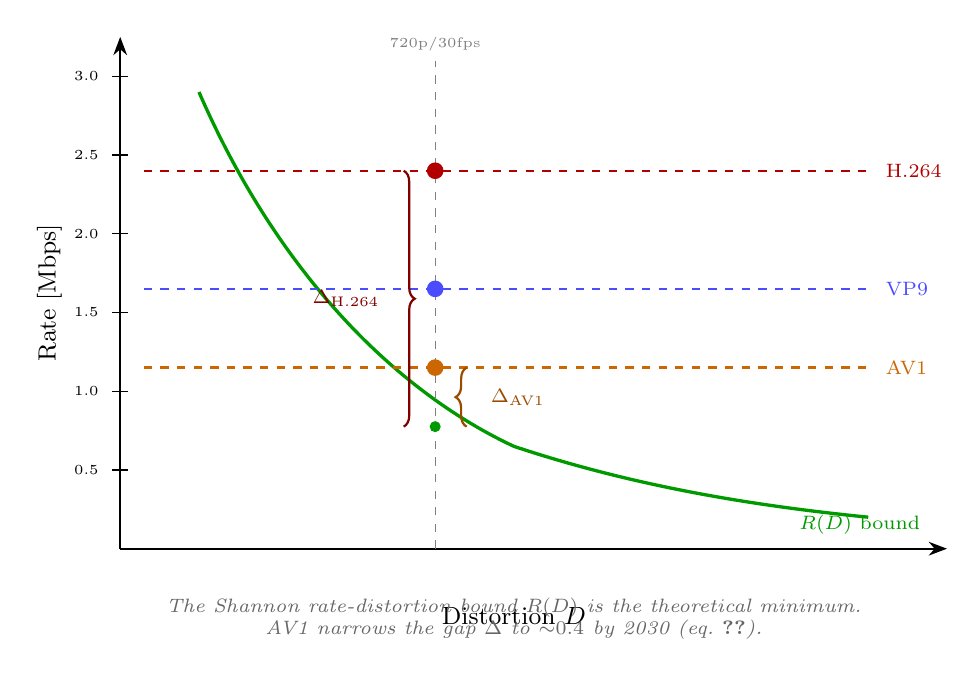
\begin{tikzpicture}[>=Stealth]

% --- Axes ---
\draw[->, thick] (0, 0) -- (10.5, 0);
\draw[->, thick] (0, 0) -- (0, 6.5);

% --- Axis titles ---
\node[font=\small] at (5, -0.85) {Distortion $D$};
\node[font=\small, rotate=90] at (-0.9, 3.25) {Rate [Mbps]};

% --- Y-axis rate labels ---
\foreach \y/\lab in {1.0/0.5, 2.0/1.0, 3.0/1.5, 4.0/2.0, 5.0/2.5, 6.0/3.0} {
  \draw (-0.1, \y) -- (0.1, \y);
  \node[font=\tiny, anchor=east] at (-0.15, \y) {\lab};
}

% --- R(D) Shannon bound curve ---
\draw[very thick, green!60!black]
  (1.0, 5.8) .. controls (2.0, 3.5) and (3.5, 2.0) ..
  (5.0, 1.3) .. controls (6.5, 0.8) and (8.0, 0.55) ..
  (9.5, 0.4);
\node[font=\scriptsize, green!60!black, anchor=north west] at (8.5, 0.55)
  {$R(D)$ bound};

% --- Reference distortion line (720p/30fps operating point) ---
\draw[thin, gray, dashed] (4.0, 0) -- (4.0, 6.2);
\node[font=\tiny, gray, anchor=south] at (4.0, 6.2) {720p/30fps};

% --- R(D) value at reference distortion ---
\fill[green!60!black] (4.0, 1.55) circle (2pt);

% --- Codec operating points at reference distortion ---
% H.264: ~2.5 Mbps
\draw[thick, dashed, red!70!black] (0.3, 4.8) -- (9.5, 4.8);
\fill[red!70!black] (4.0, 4.8) circle (3pt);
\node[font=\scriptsize, red!70!black, anchor=west] at (9.6, 4.8) {H.264};

% VP9: ~1.6 Mbps (0.65 * H.264)
\draw[thick, dashed, blue!70] (0.3, 3.3) -- (9.5, 3.3);
\fill[blue!70] (4.0, 3.3) circle (3pt);
\node[font=\scriptsize, blue!70, anchor=west] at (9.6, 3.3) {VP9};

% AV1: ~1.15 Mbps (0.46 * H.264)
\draw[thick, dashed, orange!80!black] (0.3, 2.3) -- (9.5, 2.3);
\fill[orange!80!black] (4.0, 2.3) circle (3pt);
\node[font=\scriptsize, orange!80!black, anchor=west] at (9.6, 2.3) {AV1};

% --- Gap annotations (braces) ---
% H.264 gap
\draw[decorate, decoration={brace, amplitude=4pt, mirror},
  thick, red!50!black]
  (3.6, 1.55) -- (3.6, 4.8)
  node[midway, anchor=east, font=\scriptsize, xshift=-5pt]
  {$\Delta_{\text{H.264}}$};

% AV1 gap
\draw[decorate, decoration={brace, amplitude=4pt},
  thick, orange!60!black]
  (4.4, 1.55) -- (4.4, 2.3)
  node[midway, anchor=west, font=\scriptsize, xshift=5pt]
  {$\Delta_{\text{AV1}}$};

% --- Annotation ---
\node[font=\scriptsize\itshape, text=black!60, align=center,
  anchor=north] at (5.0, -0.5)
  {The Shannon rate-distortion bound $R(D)$ is the theoretical minimum.\\
   AV1 narrows the gap $\Delta$ to ${\sim}0.4$ by 2030 (eq.~\ref{eq:coding-gap}).};

\end{tikzpicture}
\caption{Codec operating rates vs.\ the Shannon rate-distortion bound $R(D)$
  at 720p/30fps. Each codec operates above the theoretical minimum; the gap
  $\Delta$ (eq.~\ref{eq:coding-gap}) shrinks from H.264 through VP9 to AV1,
  approaching but never reaching the bound.}
\label{fig:rate-distortion}
\end{figure}

\subsubsection{Codec Entropy and WebCodecs}

The WebCodecs API (W3C Working Draft) exposes per-frame codec access,
allowing measurement and control of the instantaneous encoding rate.
For a video frame $f_t$ at time $t$, the encoder output has empirical
entropy:
\begin{equation}
  \hat{H}(f_t) = -\sum_{s \in \mathcal{S}}
    p(s \mid f_t) \log_2 p(s \mid f_t)
  \label{eq:frame-entropy}
\end{equation}
where $\mathcal{S}$ is the set of symbols emitted by the entropy coder
(CABAC for H.264/AV1, arithmetic coding for VP9). WebCodecs enables
applications to observe $|E(f_t)|$ (the encoded frame size in bits)
directly, which serves as a practical upper bound on
$\hat{H}(f_t)$:
\begin{equation}
  \hat{H}(f_t) \leq |E(f_t)| \leq R_{\text{codec}} / \text{fps}
  \label{eq:entropy-bound}
\end{equation}

\subsection{Effective Information Rate by Time Horizon}

We now combine transport and source coding measures to estimate the
effective information rate for a representative real-time video
session: a single 720p/30fps video call with one audio channel.

\excursus{Excursus: Why 720p?}{Throughout this appendix, 720p/30fps is used as
a fixed reference for cross-era comparison, not as a prediction that 720p
remains the dominant conferencing resolution. The bandwidth surplus quantified
below is precisely what enables migration to 1080p (feasible by ${\sim}$2028
with AV1 hardware encode at today's 720p bit rates) and 4K (feasible by
${\sim}$2030). The 720p baseline makes the efficiency gains legible: the same
task gets cheaper, freeing capacity for higher quality or more streams.}

Define the \emph{net information rate} as:
\begin{equation}
  I_{\text{net}} = R_{\text{codec}} \cdot \eta_{\text{transport}}
    \cdot (1 - \rho_{\text{overhead}})
    \cdot (1 - p_{\text{loss}})
  \label{eq:inet}
\end{equation}

\begin{table}[ht]
\centering
\small
\renewcommand{\arraystretch}{1.4}
\begin{tabularx}{\textwidth}{lXXX}
\toprule
\textbf{Parameter} & \textbf{March 2026} & \textbf{2027--2028} &
  \textbf{2029--2031} \\
\midrule
Median link capacity &
  120~Mbps &
  $\sim$150~Mbps &
  200--300~Mbps \\
Dominant codec (WebRTC) &
  VP9 / H.264 &
  VP9 / AV1 (HW) &
  AV1 (HW default) \\
Codec rate (720p/30fps) &
  1.5--2.5~Mbps &
  1.0--1.8~Mbps &
  0.7--1.2~Mbps \\
$\eta_{\text{transport}}$ &
  0.92 (QUIC) &
  0.93 &
  0.94 \\
$\rho_{\text{overhead}}$ (SRTP+QUIC) &
  0.06 &
  0.05 &
  0.04 \\
Typical loss $p$ &
  0.01--0.03 &
  0.01--0.02 &
  0.005--0.01 \\
$I_{\text{net}}$ (720p video) &
  1.3--2.2~Mbps &
  0.9--1.6~Mbps &
  0.6--1.1~Mbps \\
$I_{\text{net}}$ as \% of $C_{\text{link}}$ &
  1.1--1.8\% &
  0.6--1.1\% &
  0.2--0.6\% \\
\bottomrule
\end{tabularx}
\caption{Effective information rate for a 720p/30fps WebRTC video stream.
  The declining ratio $I_{\text{net}} / C_{\text{link}}$ reflects both
  improved codec efficiency and growing link capacity, freeing bandwidth
  for higher resolutions, additional streams, or concurrent data
  channels.}
\label{tab:inet}
\end{table}

The declining ratio $I_{\text{net}} / C_{\text{link}}$ in
Table~\ref{tab:inet} is the central quantitative observation: by 2030, a
720p video call consumes less than 0.5\% of available link capacity. The
surplus capacity enables qualitative changes --- 4K video conferencing,
multi-stream layouts, or concurrent data channels via WebTransport ---
that are quantitatively infeasible in 2026.

\begin{figure}[ht]
\centering
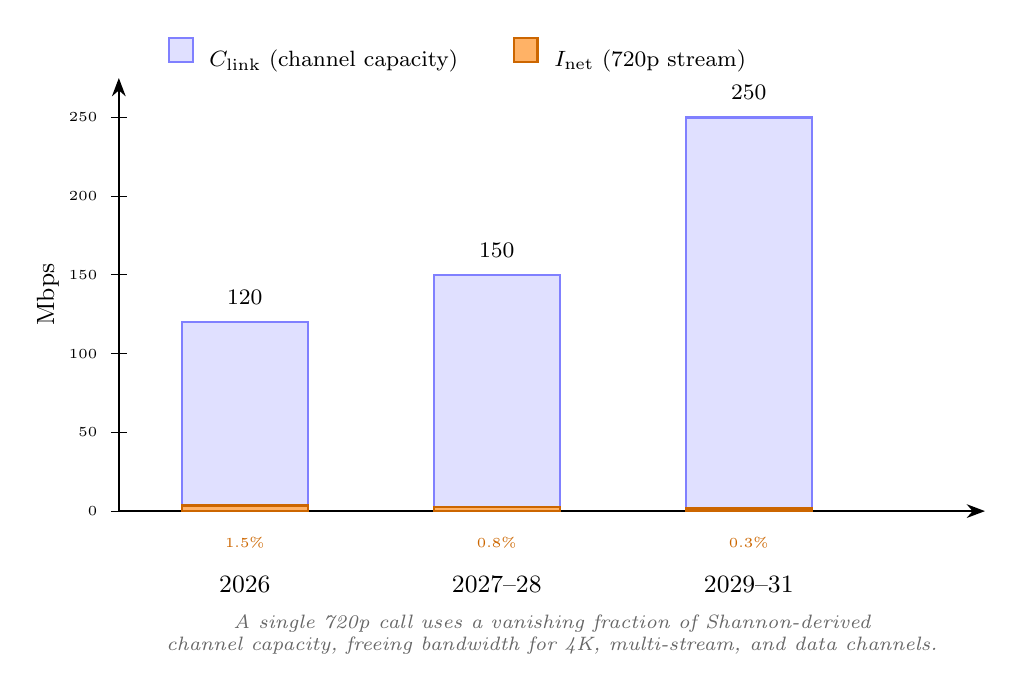
\begin{tikzpicture}[>=Stealth]

% --- Axes ---
\draw[->, thick] (0, 0) -- (11, 0);
\draw[->, thick] (0, 0) -- (0, 5.5);

% --- Axis title ---
\node[font=\small, rotate=90] at (-0.9, 2.75) {Mbps};

% --- Y-axis labels ---
\foreach \y/\lab in {0/0, 1/50, 2/100, 3/150, 4/200, 5/250} {
  \draw (-0.1, \y) -- (0.1, \y);
  \node[font=\tiny, anchor=east] at (-0.15, \y) {\lab};
}

% --- Group: March 2026 ---
% C_link = 120 Mbps -> y = 2.4
\fill[blue!12] (0.8, 0) rectangle (2.4, 2.4);
\draw[blue!50, thick] (0.8, 0) rectangle (2.4, 2.4);
% I_net = 1.75 Mbps (midpoint) -> y = 0.035
\fill[orange!60] (0.8, 0) rectangle (2.4, 0.07);
\draw[orange!80!black, thick] (0.8, 0) rectangle (2.4, 0.07);
\node[font=\footnotesize, anchor=south] at (1.6, 2.5) {120};
\node[font=\tiny, orange!80!black] at (1.6, -0.4) {1.5\%};
\node[font=\small, anchor=north] at (1.6, -0.7) {2026};

% --- Group: 2027--2028 ---
% C_link = 150 Mbps -> y = 3.0
\fill[blue!12] (4.0, 0) rectangle (5.6, 3.0);
\draw[blue!50, thick] (4.0, 0) rectangle (5.6, 3.0);
% I_net = 1.25 Mbps (midpoint) -> y = 0.025
\fill[orange!60] (4.0, 0) rectangle (5.6, 0.05);
\draw[orange!80!black, thick] (4.0, 0) rectangle (5.6, 0.05);
\node[font=\footnotesize, anchor=south] at (4.8, 3.1) {150};
\node[font=\tiny, orange!80!black] at (4.8, -0.4) {0.8\%};
\node[font=\small, anchor=north] at (4.8, -0.7) {2027--28};

% --- Group: 2029--2031 ---
% C_link = 250 Mbps -> y = 5.0
\fill[blue!12] (7.2, 0) rectangle (8.8, 5.0);
\draw[blue!50, thick] (7.2, 0) rectangle (8.8, 5.0);
% I_net = 0.85 Mbps (midpoint) -> y = 0.017
\fill[orange!60] (7.2, 0) rectangle (8.8, 0.034);
\draw[orange!80!black, thick] (7.2, 0) rectangle (8.8, 0.034);
\node[font=\footnotesize, anchor=south] at (8.0, 5.1) {250};
\node[font=\tiny, orange!80!black] at (8.0, -0.4) {0.3\%};
\node[font=\small, anchor=north] at (8.0, -0.7) {2029--31};

% --- Legend ---
\node[anchor=west, font=\footnotesize] at (0.5, 5.8) {%
  \tikz[baseline=-0.5ex]{\fill[blue!12] (0,0) rectangle (0.3,0.3);
    \draw[blue!50, thick] (0,0) rectangle (0.3,0.3);}
  ~$C_{\text{link}}$ (channel capacity) \qquad
  \tikz[baseline=-0.5ex]{\fill[orange!60] (0,0) rectangle (0.3,0.3);
    \draw[orange!80!black, thick] (0,0) rectangle (0.3,0.3);}
  ~$I_{\text{net}}$ (720p stream)};

% --- Annotation ---
\node[font=\scriptsize\itshape, text=black!60, align=center,
  anchor=north] at (5.5, -1.2)
  {A single 720p call uses a vanishing fraction of Shannon-derived\\
   channel capacity, freeing bandwidth for 4K, multi-stream, and data channels.};

\end{tikzpicture}
\caption{Channel capacity $C_{\text{link}}$ vs.\ effective information rate
  $I_{\text{net}}$ for a single 720p/30fps stream across time horizons. The
  orange bar (stream rate) is barely visible against the blue bar (capacity),
  illustrating the growing surplus as codecs improve and bandwidth increases.}
\label{fig:inet-capacity}
\end{figure}

\subsection{Security Entropy and Key Space}

The DTLS-SRTP security architecture (RFCs~8827, 3711) protects all
WebRTC media. Information-theoretic security requires that the key
entropy exceed the information content of the protected material.

For a DTLS~1.3 handshake with ECDHE on P-256, the key agreement
provides:
\begin{equation}
  H_{\text{key}} = 128 \text{~bits of security}
  \label{eq:key-entropy}
\end{equation}

The SRTP master key is 128 bits (AES-128-GCM), giving an exhaustive
search cost of $2^{128}$ operations. The total information content of a
one-hour 720p video call at 2~Mbps is:
\begin{equation}
  I_{\text{call}} = 2 \times 10^6 \times 3600
    = 7.2 \times 10^9 \text{~bits}
    \approx 2^{32.7} \text{~bits}
  \label{eq:call-content}
\end{equation}

The ratio of key entropy to protected content:
\begin{equation}
  \frac{H_{\text{key}}}{I_{\text{call}}}
    = \frac{128}{32.7} \approx 3.91
  \label{eq:security-margin}
\end{equation}

This ratio remains comfortably above~1 even for much longer sessions.
For a continuous 24-hour 4K AV1 stream at 15~Mbps:
\begin{equation}
  I_{\text{stream}} = 15 \times 10^6 \times 86400
    = 1.296 \times 10^{12} \text{~bits}
    \approx 2^{40.2} \text{~bits}
\end{equation}
yielding $H_{\text{key}} / I_{\text{stream}} \approx 3.18$, still
well above the threshold.

\subsubsection{End-to-End Encryption via Encoded Transforms}

The RTCRtpScriptTransform API (Encoded Transforms) enables
application-layer E2EE within the WebRTC pipeline. From an
information-theoretic perspective, this introduces a second encryption
layer with its own key, creating a \emph{nested channel}:
\begin{equation}
  X \xrightarrow{\;K_{\text{E2EE}}\;}
  E_1(X) \xrightarrow{\;K_{\text{SRTP}}\;}
  E_2(E_1(X))
  \label{eq:nested}
\end{equation}

The mutual information between the ciphertext and plaintext, given
neither key, satisfies:
\begin{equation}
  I\!\left(X;\, E_2(E_1(X))\right) \leq
    \min\!\big(H(K_{\text{E2EE}})^{-1},\;
    H(K_{\text{SRTP}})^{-1}\big)
    \cdot I_{\text{call}}
  \label{eq:mutual-e2ee}
\end{equation}

In practice, with $H(K_{\text{E2EE}}) = H(K_{\text{SRTP}}) = 128$
bits, this quantity is negligible ($\ll 1$ bit for any practical
session length), confirming that the nested encryption provides
information-theoretic confidentiality well beyond computational
security guarantees.

Today (March~2026), Encoded Transforms remain Chrome-only. By
2027--2028 (Section~8.3), cross-browser standardization will make
this nested channel universally available. By 2029--2031, SFrame
for group calls will extend this to $n$-party sessions, where the
mutual information between any non-member and the group plaintext
remains negligible:
\begin{equation}
  I\!\left(X;\, E(X) \;\middle|\; K_i \notin
    \{K_1, \ldots, K_n\}\right) \approx 0
  \label{eq:sframe}
\end{equation}

\subsection{WebTransport: Unreliable Datagrams and Channel Capacity}

WebTransport (RFC~9297) introduces unreliable datagrams to browser-server
communication. For latency-sensitive applications (game state, sensor
telemetry), the relevant measure is not throughput but
\emph{freshness-weighted information rate}. Define the value of a
datagram as exponentially decaying with delivery latency $\delta$:
\begin{equation}
  V(\delta) = e^{-\lambda \delta}
  \label{eq:freshness}
\end{equation}
where $\lambda > 0$ is an application-specific decay rate. The
effective information rate under unreliable delivery is:
\begin{equation}
  I_{\text{WT}} = R_{\text{send}} \cdot (1 - p_{\text{loss}})
    \cdot \mathbb{E}\!\left[e^{-\lambda \delta}\right]
  \label{eq:iwt}
\end{equation}

Under reliable delivery (TCP/WebSocket), a retransmission delays
subsequent data, so:
\begin{equation}
  I_{\text{WS}} = R_{\text{send}}
    \cdot \mathbb{E}\!\left[e^{-\lambda(\delta + p \cdot 2\tau)}\right]
  \label{eq:iws}
\end{equation}

The ratio $I_{\text{WT}} / I_{\text{WS}}$ exceeds 1 when:
\begin{equation}
  (1 - p) \cdot e^{\lambda \cdot p \cdot 2\tau} > 1
  \quad \Longleftrightarrow \quad
  \lambda > \frac{-\ln(1 - p)}{2 p \tau}
  \label{eq:wt-advantage}
\end{equation}

For $p = 0.02$ and $\tau = 25$~ms, this gives $\lambda > 20.2$~s$^{-1}$
(half-life $< 34$~ms).

\excursus{Excursus: Why $p = 0.02$ and $\tau = 25$\,ms?}{These values represent
median fixed-broadband conditions in 2026 (Table~\ref{tab:inet}). On mobile or
congested links ($p \approx 0.05$, $\tau \approx 50$\,ms), the threshold
$\lambda^*$ drops to ${\sim}10$\,s$^{-1}$, broadening WebTransport's advantage
to applications with data half-lives up to ${\sim}70$\,ms. The fixed-broadband
reference is thus conservative: mobile scenarios favor unreliable delivery even
more strongly.}

Any application where data older than
$\sim$30~ms is useless benefits from WebTransport's unreliable
mode over WebSocket --- precisely the regime of interactive gaming, live
cursor tracking, and real-time sensor feeds.

As of March~2026, Safari does not support WebTransport
(Section~5), limiting coverage to $\sim$82\%. By 2027--2028
(Section~8.2), universal support will allow applications to rely on
(\ref{eq:iwt}) without fallback paths.

\begin{figure}[ht]
\centering
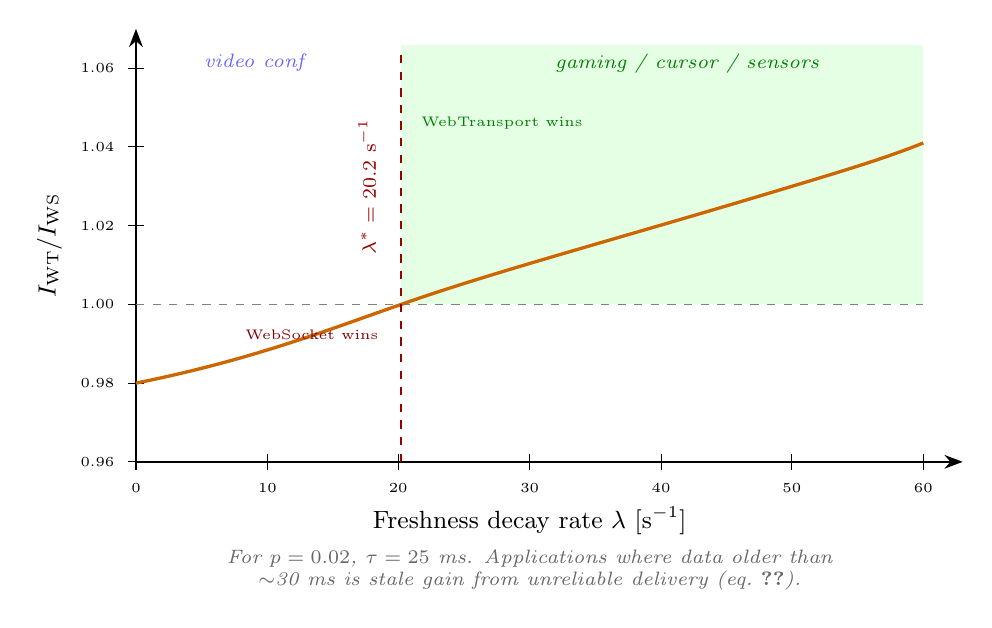
\begin{tikzpicture}[>=Stealth]

% --- Axes ---
\draw[->, thick] (0, 0) -- (10.5, 0);
\draw[->, thick] (0, 0) -- (0, 5.5);

% --- Axis titles (positioned to clear tick labels) ---
\node[font=\small] at (5, -0.75)
  {Freshness decay rate $\lambda$ [s$^{-1}$]};
\node[font=\small, rotate=90] at (-1.1, 2.75)
  {$I_{\text{WT}} / I_{\text{WS}}$};

% --- X-axis labels ---
\foreach \x/\lab in {0/0, 1.67/10, 3.33/20, 5.0/30, 6.67/40, 8.33/50, 10/60} {
  \draw (\x, -0.1) -- (\x, 0.1);
  \node[font=\tiny, anchor=north] at (\x, -0.15) {\lab};
}

% --- Y-axis labels (0.96 to 1.06, each 0.02 = 1 unit) ---
\foreach \y/\lab in {0/0.96, 1/0.98, 2/1.00, 3/1.02, 4/1.04, 5/1.06} {
  \draw (-0.1, \y) -- (0.1, \y);
  \node[font=\tiny, anchor=east] at (-0.15, \y) {\lab};
}

% --- Ratio = 1.0 line (y=2 maps to ratio 1.0) ---
\draw[thin, gray, dashed] (0, 2) -- (10, 2);

% --- Shade WebTransport advantage region ---
% lambda* = 20.2 -> x = 3.37
\fill[green!10] (3.37, 2) rectangle (10, 5.3);

% --- I_WT/I_WS curve: 0.98*exp(lambda*0.001) ---
% Y range: 0.96-1.06 (each 0.02 = 1 unit). lambda=0: y=1, lambda*=20.2: y=2, lambda=60: y=4.05
\draw[very thick, orange!80!black]
  (0, 1.0) .. controls (1.5, 1.3) and (2.5, 1.7) ..
  (3.37, 2.0) .. controls (4.5, 2.4) and (6, 2.8) ..
  (8, 3.4) .. controls (9, 3.7) and (9.5, 3.85) ..
  (10, 4.05);

% --- Threshold line ---
\draw[thick, dashed, red!60!black] (3.37, 0) -- (3.37, 5.2);
\node[font=\scriptsize, red!60!black, anchor=south, rotate=90] at (3.17, 3.5)
  {$\lambda^* = 20.2$ s$^{-1}$};

% --- Application regime labels ---
\node[font=\scriptsize\itshape, text=blue!60, anchor=north] at (1.5, 5.3)
  {video conf};
\node[font=\scriptsize\itshape, text=green!50!black, anchor=north] at (7.0, 5.3)
  {gaming / cursor / sensors};

% --- Mark advantage/disadvantage ---
\node[font=\tiny, text=red!50!black, anchor=north east] at (3.2, 1.8)
  {WebSocket wins};
\node[font=\tiny, text=green!50!black, anchor=north west] at (3.5, 4.5)
  {WebTransport wins};

% --- Annotation ---
\node[font=\scriptsize\itshape, text=black!60, align=center,
  anchor=north] at (5.0, -1.0)
  {For $p = 0.02$, $\tau = 25$~ms. Applications where data older than\\
   ${\sim}$30~ms is stale gain from unreliable delivery (eq.~\ref{eq:wt-advantage}).};

\end{tikzpicture}
\caption{Freshness-weighted information rate ratio $I_{\text{WT}} / I_{\text{WS}}$
  as a function of decay rate $\lambda$. Above the threshold $\lambda^*$,
  WebTransport's unreliable datagrams deliver more useful information per
  unit time than WebSocket's reliable delivery, because retransmission
  wastes capacity on stale data.}
\label{fig:freshness}
\end{figure}

\subsection{Projections Summary and Practical Implications}

\begin{table}[ht]
\centering
\small
\renewcommand{\arraystretch}{1.4}
\begin{tabularx}{\textwidth}{lXXX}
\toprule
\textbf{Measure} & \textbf{March 2026} & \textbf{2027--2028} &
  \textbf{2029--2031} \\
\midrule
Channel capacity $C_{\text{link}}$ &
  120~Mbps &
  150~Mbps &
  250~Mbps \\
HOL blocking factor $(1\!-\!p)^{n-2}$ at $n\!=\!8$ &
  0.94 ($p\!=\!0.01$) &
  0.94 &
  0.97 ($p\!=\!0.005$) \\
Source coding gap $\Delta$ &
  VP9: $\sim$0.8 &
  AV1 HW: $\sim$0.5 &
  AV1 opt: $\sim$0.4 \\
$I_{\text{net}}$ per 720p stream &
  1.3--2.2~Mbps &
  0.9--1.6~Mbps &
  0.6--1.1~Mbps \\
Max 720p streams in $C_{\text{link}}$ &
  $\sim$55--90 &
  $\sim$95--165 &
  $\sim$230--415 \\
E2EE availability &
  Chrome only &
  Cross-browser &
  SFrame $n$-party \\
WebTransport coverage &
  82\% &
  $\sim$100\% &
  100\% \\
Freshness threshold $\lambda^*$ &
  20.2~s$^{-1}$ &
  $\sim$18~s$^{-1}$ &
  $\sim$15~s$^{-1}$ \\
\bottomrule
\end{tabularx}
\caption{Information-theoretic measures across time horizons. $\Delta$
  is the coding efficiency gap (\ref{eq:coding-gap}), $I_{\text{net}}$
  is the net information rate (\ref{eq:inet}), and $\lambda^*$ is the
  freshness decay threshold above which WebTransport dominates WebSocket
  (\ref{eq:wt-advantage}).}
\label{tab:projections}
\end{table}

The trajectory is clear: the combination of improving source coding
(AV1 hardware), expanding channel capacity (broadband growth), and
maturing transport protocols (QUIC universal, WebTransport universal)
drives the \emph{information cost per unit of communicated experience}
steadily downward. The remaining question is not whether the
Shannon capacity suffices --- it already does, by orders of magnitude
--- but how efficiently the protocol stack converts that capacity into
delivered, fresh, secure information at the application layer. By
2030, the gap between theoretical capacity and realized throughput will
be the narrowest it has ever been for browser-based real-time
communication.

\subsubsection{What the Theory Means for Applications}

The equations and figures in this appendix are not purely academic. Each
theoretical result maps to a concrete design decision that application
developers face today and over the next five years.

\textbf{Codec selection determines bandwidth cost, not quality.}
The rate-distortion analysis (Section~A.2, Figure~\ref{fig:rate-distortion})
shows that AV1 operates at roughly 46\% of H.264's bit rate for equivalent
perceptual quality at 720p. In practice, this means a WebRTC application
switching from H.264 to AV1 can either halve its bandwidth consumption at
the same quality or substantially increase resolution (e.g., 720p to 1080p)
within the same bandwidth envelope. By 2030, with AV1 hardware encoding
ubiquitous and the coding gap $\Delta$ approaching 0.4, further codec
improvements yield diminishing returns --- the stack will be operating close
enough to the Shannon rate-distortion bound that the next generation of
efficiency gains will come from transport and architecture, not codecs alone.

\textbf{QUIC's advantage is situational but decisive on bad networks.}
The head-of-line blocking analysis (Section~A.1.1,
Figure~\ref{fig:hol-blocking}) shows that QUIC's per-stream throughput
advantage over TCP is modest on good networks (6\% at 1\% loss) but
substantial on degraded ones (34\% at 5\% loss). The practical implication
is that applications targeting mobile users, emerging markets, or congested
enterprise networks --- precisely the environments where real-time
communication is hardest --- benefit disproportionately from QUIC-based
transports. For a video conference with 8 participants on a cellular
connection experiencing 3--5\% packet loss, the difference between QUIC and
TCP is the difference between usable and degraded video.

\textbf{Connection latency is a solved problem for returning users.}
The handshake analysis (Section~A.1.2) shows that QUIC 0-RTT eliminates
connection establishment overhead entirely for resumed connections. For a
WebTransport application that a user opens daily --- a collaboration tool,
a live dashboard, a recurring meeting client --- the time to first useful
byte drops to zero. The 1.125~MB of wasted capacity during a TCP+TLS
handshake on a 120~Mbps link may seem small, but for latency-sensitive
applications where the first 100~ms of perceived responsiveness determines
user experience, the difference is measurable.

\textbf{Bandwidth surplus enables architectural ambition.}
The effective information rate analysis (Section~A.3,
Figure~\ref{fig:inet-capacity}) reveals the most consequential practical
finding: a single 720p video stream consumes a vanishing fraction of
available link capacity (under 0.5\% by 2030). This surplus is not merely
``headroom'' --- it is the resource that makes new application architectures
feasible. A 250~Mbps link can theoretically carry 230--415 simultaneous 720p
streams. In practice, this means applications can afford to run multiple
concurrent media flows (video, screen share, spatial audio), data channels
(collaborative editing, file transfer), and telemetry streams without
contending for bandwidth. The constraint shifts from ``can the network carry
this?''\ to ``can the application manage this complexity?''

\textbf{End-to-end encryption adds negligible overhead.}
The security analysis (Section~A.4) confirms that the nested DTLS-SRTP plus
E2EE architecture imposes no meaningful information-theoretic cost. The key
entropy ($2^{128}$) exceeds the information content of any practical session
by a factor of at least 3. For application developers, this means E2EE can
be treated as a default rather than a premium feature --- there is no
bandwidth, latency, or capacity penalty for encrypting at the application
layer on top of the transport-layer encryption that WebRTC already mandates.
The only constraint is API availability, which moves from Chrome-only (2026)
to universal (2028).

\textbf{WebTransport unlocks real-time data that WebSocket cannot serve.}
The freshness analysis (Section~A.5, Figure~\ref{fig:freshness}) quantifies
when unreliable delivery outperforms reliable delivery: any data with a
useful half-life below approximately 34~ms benefits from WebTransport's
unreliable datagrams. This covers a wide class of interactive applications
--- game state synchronization, live cursor and pointer sharing, real-time
sensor feeds, collaborative whiteboard strokes --- where retransmitting a
stale update is worse than dropping it. Before WebTransport, these
applications had to choose between WebSocket (reliable but stale under loss)
and WebRTC DataChannel (unreliable mode available but requiring the full
peer-to-peer ICE/DTLS machinery). WebTransport provides the unreliable
mode with a simple client-server model over HTTP/3, removing the
architectural overhead.

\textbf{The overall picture: the stack converges on efficiency.}
Taken together, the information-theoretic measures trace a consistent
trajectory. The protocol stack is converging toward the theoretical limits
established by Shannon: codecs approach the rate-distortion bound, transports
eliminate unnecessary blocking and handshake overhead, and encryption adds
negligible cost. By 2030, the practical distance between what the standards
deliver and what information theory permits will be the smallest it has ever
been for browser-based real-time communication. The consequence for
application developers is that the infrastructure --- standards, hardware,
and networks --- will no longer be the binding constraint. The remaining
challenge is purely architectural: how to compose these efficient, universal
primitives into applications that fully exploit the capacity and low latency
they provide.

%
% Requires in the preamble: amsmath, amssymb, tabularx, booktabs

\section{Information-Theoretic View}
\label{app:info-theory}

This appendix applies information-theoretic measures to the real-time
web communication stack described in this document. We quantify channel
capacity, source coding efficiency, and effective information rates
across three time horizons: today (March~2026), the near term
(2027--2028), and the medium term (2029--2031). The analysis draws on
the standards, codec parameters, and infrastructure projections
developed in the main text.

\subsection{Channel Capacity of the Transport Layer}

The Shannon-Hartley theorem gives the theoretical maximum information
rate for a channel with additive white Gaussian noise:
\begin{equation}
  C = B \log_2\!\left(1 + \frac{S}{N}\right) \quad \text{[bits/s]}
  \label{eq:shannon}
\end{equation}
where $B$ is the channel bandwidth in Hz and $S/N$ is the
signal-to-noise ratio.

While the physical-layer capacity of a broadband link is governed by
(\ref{eq:shannon}), the \emph{effective} capacity available to the
application is reduced by protocol overhead, congestion control, and
transport inefficiencies. We define the effective application-layer
throughput as:
\begin{equation}
  R_{\text{eff}} = C_{\text{link}} \cdot \eta_{\text{transport}}
    \cdot (1 - \rho_{\text{overhead}})
  \label{eq:reff}
\end{equation}
where $C_{\text{link}}$ is the link-layer capacity,
$\eta_{\text{transport}} \in (0,1]$ is the transport efficiency factor
(capturing congestion control, retransmission, and multiplexing
behavior), and $\rho_{\text{overhead}} \in [0,1)$ is the fractional
protocol overhead (headers, encryption, framing).

\subsubsection{Head-of-Line Blocking and Multiplexed Capacity}

Consider $n$ independent streams multiplexed over a single connection.
Under TCP (HTTP/2), a single lost packet blocks all $n$ streams. The
expected throughput per stream under loss rate $p$ is bounded by:
\begin{equation}
  R_{\text{TCP}}^{(i)} \leq \frac{R_{\text{eff}}}{n}
    \cdot (1 - p)^{n-1}
  \label{eq:hol-tcp}
\end{equation}
because a loss in \emph{any} of the $n$ streams stalls all others. Under
QUIC (RFC~9000), streams are independent at the transport layer, so:
\begin{equation}
  R_{\text{QUIC}}^{(i)} \leq \frac{R_{\text{eff}}}{n}
    \cdot (1 - p)
  \label{eq:hol-quic}
\end{equation}
The ratio of effective per-stream throughput is:
\begin{equation}
  \frac{R_{\text{QUIC}}^{(i)}}{R_{\text{TCP}}^{(i)}}
    = \frac{1}{(1-p)^{n-2}}
  \label{eq:hol-ratio}
\end{equation}
\excursus{Excursus: Why $n = 8$?}{In a typical multi-participant video
conference, each peer contributes multiple concurrent streams: a camera video
track, an audio track, and often a screen-share or data channel. A four-person
call with two media tracks each produces $n = 8$ multiplexed streams over a
single connection --- the reference value used throughout this section. Larger
meetings (e.g.\ 10 participants with simulcast layers) push $n$ higher,
amplifying the HOL blocking effect further.}

For $n = 8$ streams (a typical multi-track video conference) at
$p = 0.01$ (1\% loss), this gives a QUIC advantage factor of
$1/(0.99)^6 \approx 1.062$, a modest 6.2\% improvement. At $p = 0.05$
(5\% loss, common on mobile or congested links), the factor is
$1/(0.95)^6 \approx 1.34$, a 34\% throughput advantage per stream.

\begin{figure}[ht]
\centering
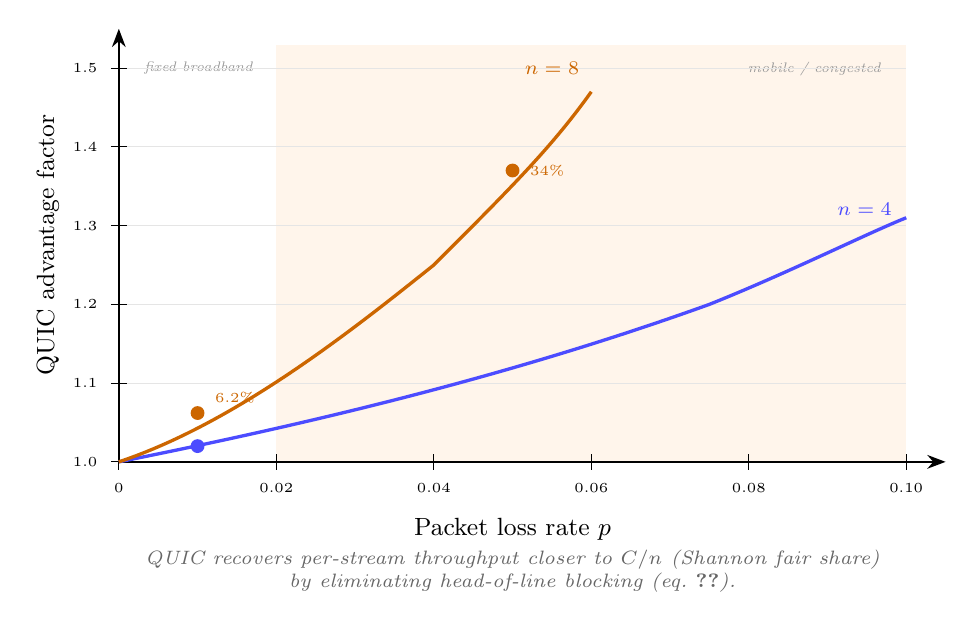
\begin{tikzpicture}[>=Stealth]

% --- Shaded region (drawn FIRST so curves appear on top) ---
\fill[orange!8] (2, 0) rectangle (10, 5.3);
\node[font=\tiny\itshape, text=black!40, anchor=north east] at (9.8, 5.2)
  {mobile / congested};
\node[font=\tiny\itshape, text=black!40, anchor=north west] at (0.2, 5.2)
  {fixed broadband};

% --- Grid lines ---
\foreach \y in {1, 2, 3, 4, 5} {
  \draw[gray!20] (0, \y) -- (10, \y);
}

% --- Axes ---
\draw[->, thick] (0, 0) -- (10.5, 0);
\draw[->, thick] (0, 0) -- (0, 5.5);

% --- Axis titles (positioned to clear tick labels) ---
\node[font=\small] at (5, -0.85) {Packet loss rate $p$};
\node[font=\small, rotate=90] at (-0.9, 2.75) {QUIC advantage factor};

% --- X-axis labels ---
\foreach \x/\lab in {0/0, 2/0.02, 4/0.04, 6/0.06, 8/0.08, 10/0.10} {
  \draw (\x, -0.1) -- (\x, 0.1);
  \node[font=\tiny, anchor=north] at (\x, -0.15) {\lab};
}

% --- Y-axis labels ---
\foreach \y/\lab in {0/1.0, 1/1.1, 2/1.2, 3/1.3, 4/1.4, 5/1.5} {
  \draw (-0.1, \y) -- (0.1, \y);
  \node[font=\tiny, anchor=east] at (-0.15, \y) {\lab};
}

% --- n=4 curve: 1/(1-p)^2 ---
\draw[very thick, blue!70]
  (0, 0) .. controls (2.5, 0.5) and (5, 1.1) ..
  (7.5, 2.0) .. controls (8.5, 2.4) and (9.5, 2.9) ..
  (10, 3.1);
\node[font=\scriptsize, blue!70, anchor=south west] at (9.0, 3.0)
  {$n = 4$};

% --- n=8 curve: 1/(1-p)^6 ---
\draw[very thick, orange!80!black]
  (0, 0) .. controls (1.5, 0.5) and (3, 1.7) ..
  (4, 2.5) .. controls (5, 3.5) and (5.5, 4.0) ..
  (6, 4.7);
\node[font=\scriptsize, orange!80!black, anchor=south] at (5.5, 4.8)
  {$n = 8$};

% --- Reference points ---
\fill[orange!80!black] (1.0, 0.62) circle (2.5pt);
\node[font=\tiny, orange!80!black, anchor=south west] at (1.1, 0.62)
  {6.2\%};

\fill[orange!80!black] (5.0, 3.7) circle (2.5pt);
\node[font=\tiny, orange!80!black, anchor=west] at (5.1, 3.7)
  {34\%};

\fill[blue!70] (1.0, 0.20) circle (2.5pt);

% --- Annotation ---
\node[font=\scriptsize\itshape, text=black!60, align=center,
  anchor=north] at (5.0, -1.0)
  {QUIC recovers per-stream throughput closer to $C/n$ (Shannon fair share)\\
   by eliminating head-of-line blocking (eq.~\ref{eq:hol-ratio}).};

\end{tikzpicture}
\caption{QUIC advantage factor $1/(1-p)^{n-2}$ over TCP for multiplexed
  streams. At 5\% loss with $n=8$ streams, QUIC delivers 34\% more
  per-stream throughput by maintaining independence at the transport layer.}
\label{fig:hol-blocking}
\end{figure}

\subsubsection{Connection Establishment Latency}

Let $\tau$ denote the one-way latency (half the round-trip time). The
information-carrying capacity during connection establishment is zero;
the handshake represents pure overhead. The time to first useful byte
is:
\begin{align}
  T_{\text{TCP+TLS\,1.3}} &= 2\tau_{\text{TCP}} + \tau_{\text{TLS}}
    = 3\tau \quad \text{(1-RTT TLS~1.3)} \label{eq:tcp-setup} \\
  T_{\text{QUIC}} &= \tau \quad \text{(1-RTT)}
    \label{eq:quic-setup} \\
  T_{\text{QUIC,\,0-RTT}} &= 0 \quad \text{(resumption)}
    \label{eq:quic-0rtt}
\end{align}
The QUIC 0-RTT case (\ref{eq:quic-0rtt}) eliminates the handshake
entirely for resumed connections. The information lost during
handshake dead time, relative to steady-state capacity, is:
\begin{equation}
  I_{\text{lost}} = C_{\text{link}} \cdot T_{\text{setup}}
  \label{eq:ilost}
\end{equation}
For a 120~Mbps link with $\tau = 25$~ms (typical fixed broadband in
2026), the TCP+TLS~1.3 handshake wastes $120 \times 10^6 \times 0.075
= 9 \times 10^6$ bits (1.125~MB), while QUIC~1-RTT wastes only
$3 \times 10^6$ bits (375~KB).

\subsection{Source Coding Efficiency}

The rate-distortion function $R(D)$ defines the minimum bit rate
required to represent a source at distortion level $D$. For a
Gaussian source with variance $\sigma^2$ under mean squared error
distortion:
\begin{equation}
  R(D) = \frac{1}{2} \log_2 \frac{\sigma^2}{D}
    \quad \text{[bits/sample]}
  \label{eq:rate-distortion}
\end{equation}

\excursus{Excursus: Why Gaussian source?}{The Gaussian memoryless model is used
because it yields the highest (worst-case) $R(D)$ among all sources of equal
variance. Any codec that approaches the Gaussian bound on real video is
therefore doing at least as well as the bound predicts --- the true $R(D)$ for
spatially and temporally correlated video lies below the Gaussian curve, making
it a conservative benchmark.}

No practical codec achieves $R(D)$;\footnote{The $R(D)$ curve in
Figure~\ref{fig:rate-distortion} is the Gaussian memoryless source bound
(equation~\ref{eq:rate-distortion}), which is an upper bound on the true
$R(D)$ for non-Gaussian sources such as video.  Additionally, $R(D)$ assumes
zero excess-distortion probability, whereas practical codecs permit a
frame-level excess-distortion probability on the order of $10^{-6}$ to
$10^{-8}$.  Both factors allow codec operating points measured on real content
to approach or marginally cross the Gaussian bound.} real codecs operate at
some rate $R_{\text{codec}} > R(D)$. We define the coding efficiency gap as:
\begin{equation}
  \Delta = \frac{R_{\text{codec}} - R(D)}{R(D)}
  \label{eq:coding-gap}
\end{equation}

The codecs in the WebRTC stack can be ordered by their empirical
proximity to $R(D)$ for typical video content at conversational
resolutions (720p, 30~fps). Using published Bj\o ntegaard Delta (BD)
rate measurements:
\begin{equation}
  R_{\text{H.264}} > R_{\text{VP9}} > R_{\text{AV1}}
    > R(D)
  \label{eq:codec-ordering}
\end{equation}

Specifically, the empirical rate savings at equivalent PSNR are
approximately:
\begin{align}
  R_{\text{VP9}}  &\approx 0.65 \cdot R_{\text{H.264}}
    \quad (\sim\!35\% \text{ savings}) \label{eq:vp9-savings} \\
  R_{\text{AV1}}  &\approx 0.70 \cdot R_{\text{VP9}}
    \approx 0.46 \cdot R_{\text{H.264}}
    \quad (\sim\!30\% \text{ over VP9})
  \label{eq:av1-savings}
\end{align}

\begin{figure}[ht]
\centering
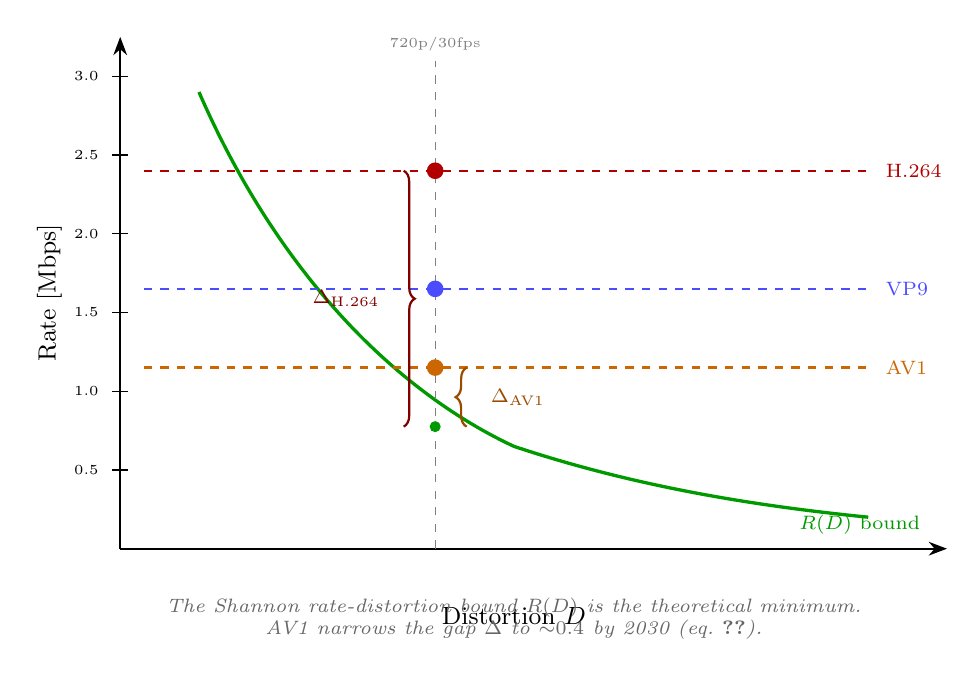
\begin{tikzpicture}[>=Stealth]

% --- Axes ---
\draw[->, thick] (0, 0) -- (10.5, 0);
\draw[->, thick] (0, 0) -- (0, 6.5);

% --- Axis titles ---
\node[font=\small] at (5, -0.85) {Distortion $D$};
\node[font=\small, rotate=90] at (-0.9, 3.25) {Rate [Mbps]};

% --- Y-axis rate labels ---
\foreach \y/\lab in {1.0/0.5, 2.0/1.0, 3.0/1.5, 4.0/2.0, 5.0/2.5, 6.0/3.0} {
  \draw (-0.1, \y) -- (0.1, \y);
  \node[font=\tiny, anchor=east] at (-0.15, \y) {\lab};
}

% --- R(D) Shannon bound curve ---
\draw[very thick, green!60!black]
  (1.0, 5.8) .. controls (2.0, 3.5) and (3.5, 2.0) ..
  (5.0, 1.3) .. controls (6.5, 0.8) and (8.0, 0.55) ..
  (9.5, 0.4);
\node[font=\scriptsize, green!60!black, anchor=north west] at (8.5, 0.55)
  {$R(D)$ bound};

% --- Reference distortion line (720p/30fps operating point) ---
\draw[thin, gray, dashed] (4.0, 0) -- (4.0, 6.2);
\node[font=\tiny, gray, anchor=south] at (4.0, 6.2) {720p/30fps};

% --- R(D) value at reference distortion ---
\fill[green!60!black] (4.0, 1.55) circle (2pt);

% --- Codec operating points at reference distortion ---
% H.264: ~2.5 Mbps
\draw[thick, dashed, red!70!black] (0.3, 4.8) -- (9.5, 4.8);
\fill[red!70!black] (4.0, 4.8) circle (3pt);
\node[font=\scriptsize, red!70!black, anchor=west] at (9.6, 4.8) {H.264};

% VP9: ~1.6 Mbps (0.65 * H.264)
\draw[thick, dashed, blue!70] (0.3, 3.3) -- (9.5, 3.3);
\fill[blue!70] (4.0, 3.3) circle (3pt);
\node[font=\scriptsize, blue!70, anchor=west] at (9.6, 3.3) {VP9};

% AV1: ~1.15 Mbps (0.46 * H.264)
\draw[thick, dashed, orange!80!black] (0.3, 2.3) -- (9.5, 2.3);
\fill[orange!80!black] (4.0, 2.3) circle (3pt);
\node[font=\scriptsize, orange!80!black, anchor=west] at (9.6, 2.3) {AV1};

% --- Gap annotations (braces) ---
% H.264 gap
\draw[decorate, decoration={brace, amplitude=4pt, mirror},
  thick, red!50!black]
  (3.6, 1.55) -- (3.6, 4.8)
  node[midway, anchor=east, font=\scriptsize, xshift=-5pt]
  {$\Delta_{\text{H.264}}$};

% AV1 gap
\draw[decorate, decoration={brace, amplitude=4pt},
  thick, orange!60!black]
  (4.4, 1.55) -- (4.4, 2.3)
  node[midway, anchor=west, font=\scriptsize, xshift=5pt]
  {$\Delta_{\text{AV1}}$};

% --- Annotation ---
\node[font=\scriptsize\itshape, text=black!60, align=center,
  anchor=north] at (5.0, -0.5)
  {The Shannon rate-distortion bound $R(D)$ is the theoretical minimum.\\
   AV1 narrows the gap $\Delta$ to ${\sim}0.4$ by 2030 (eq.~\ref{eq:coding-gap}).};

\end{tikzpicture}
\caption{Codec operating rates vs.\ the Shannon rate-distortion bound $R(D)$
  at 720p/30fps. Each codec operates above the theoretical minimum; the gap
  $\Delta$ (eq.~\ref{eq:coding-gap}) shrinks from H.264 through VP9 to AV1,
  approaching but never reaching the bound.}
\label{fig:rate-distortion}
\end{figure}

\subsubsection{Codec Entropy and WebCodecs}

The WebCodecs API (W3C Working Draft) exposes per-frame codec access,
allowing measurement and control of the instantaneous encoding rate.
For a video frame $f_t$ at time $t$, the encoder output has empirical
entropy:
\begin{equation}
  \hat{H}(f_t) = -\sum_{s \in \mathcal{S}}
    p(s \mid f_t) \log_2 p(s \mid f_t)
  \label{eq:frame-entropy}
\end{equation}
where $\mathcal{S}$ is the set of symbols emitted by the entropy coder
(CABAC for H.264/AV1, arithmetic coding for VP9). WebCodecs enables
applications to observe $|E(f_t)|$ (the encoded frame size in bits)
directly, which serves as a practical upper bound on
$\hat{H}(f_t)$:
\begin{equation}
  \hat{H}(f_t) \leq |E(f_t)| \leq R_{\text{codec}} / \text{fps}
  \label{eq:entropy-bound}
\end{equation}

\subsection{Effective Information Rate by Time Horizon}

We now combine transport and source coding measures to estimate the
effective information rate for a representative real-time video
session: a single 720p/30fps video call with one audio channel.

\excursus{Excursus: Why 720p?}{Throughout this appendix, 720p/30fps is used as
a fixed reference for cross-era comparison, not as a prediction that 720p
remains the dominant conferencing resolution. The bandwidth surplus quantified
below is precisely what enables migration to 1080p (feasible by ${\sim}$2028
with AV1 hardware encode at today's 720p bit rates) and 4K (feasible by
${\sim}$2030). The 720p baseline makes the efficiency gains legible: the same
task gets cheaper, freeing capacity for higher quality or more streams.}

Define the \emph{net information rate} as:
\begin{equation}
  I_{\text{net}} = R_{\text{codec}} \cdot \eta_{\text{transport}}
    \cdot (1 - \rho_{\text{overhead}})
    \cdot (1 - p_{\text{loss}})
  \label{eq:inet}
\end{equation}

\begin{table}[ht]
\centering
\small
\renewcommand{\arraystretch}{1.4}
\begin{tabularx}{\textwidth}{lXXX}
\toprule
\textbf{Parameter} & \textbf{March 2026} & \textbf{2027--2028} &
  \textbf{2029--2031} \\
\midrule
Median link capacity &
  120~Mbps &
  $\sim$150~Mbps &
  200--300~Mbps \\
Dominant codec (WebRTC) &
  VP9 / H.264 &
  VP9 / AV1 (HW) &
  AV1 (HW default) \\
Codec rate (720p/30fps) &
  1.5--2.5~Mbps &
  1.0--1.8~Mbps &
  0.7--1.2~Mbps \\
$\eta_{\text{transport}}$ &
  0.92 (QUIC) &
  0.93 &
  0.94 \\
$\rho_{\text{overhead}}$ (SRTP+QUIC) &
  0.06 &
  0.05 &
  0.04 \\
Typical loss $p$ &
  0.01--0.03 &
  0.01--0.02 &
  0.005--0.01 \\
$I_{\text{net}}$ (720p video) &
  1.3--2.2~Mbps &
  0.9--1.6~Mbps &
  0.6--1.1~Mbps \\
$I_{\text{net}}$ as \% of $C_{\text{link}}$ &
  1.1--1.8\% &
  0.6--1.1\% &
  0.2--0.6\% \\
\bottomrule
\end{tabularx}
\caption{Effective information rate for a 720p/30fps WebRTC video stream.
  The declining ratio $I_{\text{net}} / C_{\text{link}}$ reflects both
  improved codec efficiency and growing link capacity, freeing bandwidth
  for higher resolutions, additional streams, or concurrent data
  channels.}
\label{tab:inet}
\end{table}

The declining ratio $I_{\text{net}} / C_{\text{link}}$ in
Table~\ref{tab:inet} is the central quantitative observation: by 2030, a
720p video call consumes less than 0.5\% of available link capacity. The
surplus capacity enables qualitative changes --- 4K video conferencing,
multi-stream layouts, or concurrent data channels via WebTransport ---
that are quantitatively infeasible in 2026.

\begin{figure}[ht]
\centering
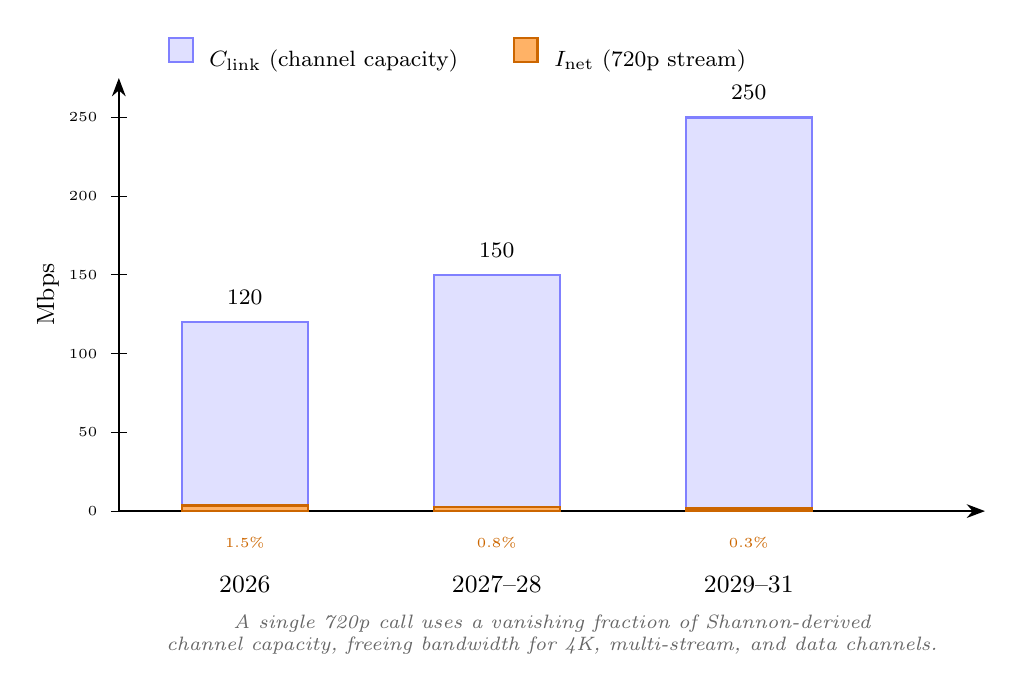
\begin{tikzpicture}[>=Stealth]

% --- Axes ---
\draw[->, thick] (0, 0) -- (11, 0);
\draw[->, thick] (0, 0) -- (0, 5.5);

% --- Axis title ---
\node[font=\small, rotate=90] at (-0.9, 2.75) {Mbps};

% --- Y-axis labels ---
\foreach \y/\lab in {0/0, 1/50, 2/100, 3/150, 4/200, 5/250} {
  \draw (-0.1, \y) -- (0.1, \y);
  \node[font=\tiny, anchor=east] at (-0.15, \y) {\lab};
}

% --- Group: March 2026 ---
% C_link = 120 Mbps -> y = 2.4
\fill[blue!12] (0.8, 0) rectangle (2.4, 2.4);
\draw[blue!50, thick] (0.8, 0) rectangle (2.4, 2.4);
% I_net = 1.75 Mbps (midpoint) -> y = 0.035
\fill[orange!60] (0.8, 0) rectangle (2.4, 0.07);
\draw[orange!80!black, thick] (0.8, 0) rectangle (2.4, 0.07);
\node[font=\footnotesize, anchor=south] at (1.6, 2.5) {120};
\node[font=\tiny, orange!80!black] at (1.6, -0.4) {1.5\%};
\node[font=\small, anchor=north] at (1.6, -0.7) {2026};

% --- Group: 2027--2028 ---
% C_link = 150 Mbps -> y = 3.0
\fill[blue!12] (4.0, 0) rectangle (5.6, 3.0);
\draw[blue!50, thick] (4.0, 0) rectangle (5.6, 3.0);
% I_net = 1.25 Mbps (midpoint) -> y = 0.025
\fill[orange!60] (4.0, 0) rectangle (5.6, 0.05);
\draw[orange!80!black, thick] (4.0, 0) rectangle (5.6, 0.05);
\node[font=\footnotesize, anchor=south] at (4.8, 3.1) {150};
\node[font=\tiny, orange!80!black] at (4.8, -0.4) {0.8\%};
\node[font=\small, anchor=north] at (4.8, -0.7) {2027--28};

% --- Group: 2029--2031 ---
% C_link = 250 Mbps -> y = 5.0
\fill[blue!12] (7.2, 0) rectangle (8.8, 5.0);
\draw[blue!50, thick] (7.2, 0) rectangle (8.8, 5.0);
% I_net = 0.85 Mbps (midpoint) -> y = 0.017
\fill[orange!60] (7.2, 0) rectangle (8.8, 0.034);
\draw[orange!80!black, thick] (7.2, 0) rectangle (8.8, 0.034);
\node[font=\footnotesize, anchor=south] at (8.0, 5.1) {250};
\node[font=\tiny, orange!80!black] at (8.0, -0.4) {0.3\%};
\node[font=\small, anchor=north] at (8.0, -0.7) {2029--31};

% --- Legend ---
\node[anchor=west, font=\footnotesize] at (0.5, 5.8) {%
  \tikz[baseline=-0.5ex]{\fill[blue!12] (0,0) rectangle (0.3,0.3);
    \draw[blue!50, thick] (0,0) rectangle (0.3,0.3);}
  ~$C_{\text{link}}$ (channel capacity) \qquad
  \tikz[baseline=-0.5ex]{\fill[orange!60] (0,0) rectangle (0.3,0.3);
    \draw[orange!80!black, thick] (0,0) rectangle (0.3,0.3);}
  ~$I_{\text{net}}$ (720p stream)};

% --- Annotation ---
\node[font=\scriptsize\itshape, text=black!60, align=center,
  anchor=north] at (5.5, -1.2)
  {A single 720p call uses a vanishing fraction of Shannon-derived\\
   channel capacity, freeing bandwidth for 4K, multi-stream, and data channels.};

\end{tikzpicture}
\caption{Channel capacity $C_{\text{link}}$ vs.\ effective information rate
  $I_{\text{net}}$ for a single 720p/30fps stream across time horizons. The
  orange bar (stream rate) is barely visible against the blue bar (capacity),
  illustrating the growing surplus as codecs improve and bandwidth increases.}
\label{fig:inet-capacity}
\end{figure}

\subsection{Security Entropy and Key Space}

The DTLS-SRTP security architecture (RFCs~8827, 3711) protects all
WebRTC media. Information-theoretic security requires that the key
entropy exceed the information content of the protected material.

For a DTLS~1.3 handshake with ECDHE on P-256, the key agreement
provides:
\begin{equation}
  H_{\text{key}} = 128 \text{~bits of security}
  \label{eq:key-entropy}
\end{equation}

The SRTP master key is 128 bits (AES-128-GCM), giving an exhaustive
search cost of $2^{128}$ operations. The total information content of a
one-hour 720p video call at 2~Mbps is:
\begin{equation}
  I_{\text{call}} = 2 \times 10^6 \times 3600
    = 7.2 \times 10^9 \text{~bits}
    \approx 2^{32.7} \text{~bits}
  \label{eq:call-content}
\end{equation}

The ratio of key entropy to protected content:
\begin{equation}
  \frac{H_{\text{key}}}{I_{\text{call}}}
    = \frac{128}{32.7} \approx 3.91
  \label{eq:security-margin}
\end{equation}

This ratio remains comfortably above~1 even for much longer sessions.
For a continuous 24-hour 4K AV1 stream at 15~Mbps:
\begin{equation}
  I_{\text{stream}} = 15 \times 10^6 \times 86400
    = 1.296 \times 10^{12} \text{~bits}
    \approx 2^{40.2} \text{~bits}
\end{equation}
yielding $H_{\text{key}} / I_{\text{stream}} \approx 3.18$, still
well above the threshold.

\subsubsection{End-to-End Encryption via Encoded Transforms}

The RTCRtpScriptTransform API (Encoded Transforms) enables
application-layer E2EE within the WebRTC pipeline. From an
information-theoretic perspective, this introduces a second encryption
layer with its own key, creating a \emph{nested channel}:
\begin{equation}
  X \xrightarrow{\;K_{\text{E2EE}}\;}
  E_1(X) \xrightarrow{\;K_{\text{SRTP}}\;}
  E_2(E_1(X))
  \label{eq:nested}
\end{equation}

The mutual information between the ciphertext and plaintext, given
neither key, satisfies:
\begin{equation}
  I\!\left(X;\, E_2(E_1(X))\right) \leq
    \min\!\big(H(K_{\text{E2EE}})^{-1},\;
    H(K_{\text{SRTP}})^{-1}\big)
    \cdot I_{\text{call}}
  \label{eq:mutual-e2ee}
\end{equation}

In practice, with $H(K_{\text{E2EE}}) = H(K_{\text{SRTP}}) = 128$
bits, this quantity is negligible ($\ll 1$ bit for any practical
session length), confirming that the nested encryption provides
information-theoretic confidentiality well beyond computational
security guarantees.

Today (March~2026), Encoded Transforms remain Chrome-only. By
2027--2028 (Section~8.3), cross-browser standardization will make
this nested channel universally available. By 2029--2031, SFrame
for group calls will extend this to $n$-party sessions, where the
mutual information between any non-member and the group plaintext
remains negligible:
\begin{equation}
  I\!\left(X;\, E(X) \;\middle|\; K_i \notin
    \{K_1, \ldots, K_n\}\right) \approx 0
  \label{eq:sframe}
\end{equation}

\subsection{WebTransport: Unreliable Datagrams and Channel Capacity}

WebTransport (RFC~9297) introduces unreliable datagrams to browser-server
communication. For latency-sensitive applications (game state, sensor
telemetry), the relevant measure is not throughput but
\emph{freshness-weighted information rate}. Define the value of a
datagram as exponentially decaying with delivery latency $\delta$:
\begin{equation}
  V(\delta) = e^{-\lambda \delta}
  \label{eq:freshness}
\end{equation}
where $\lambda > 0$ is an application-specific decay rate. The
effective information rate under unreliable delivery is:
\begin{equation}
  I_{\text{WT}} = R_{\text{send}} \cdot (1 - p_{\text{loss}})
    \cdot \mathbb{E}\!\left[e^{-\lambda \delta}\right]
  \label{eq:iwt}
\end{equation}

Under reliable delivery (TCP/WebSocket), a retransmission delays
subsequent data, so:
\begin{equation}
  I_{\text{WS}} = R_{\text{send}}
    \cdot \mathbb{E}\!\left[e^{-\lambda(\delta + p \cdot 2\tau)}\right]
  \label{eq:iws}
\end{equation}

The ratio $I_{\text{WT}} / I_{\text{WS}}$ exceeds 1 when:
\begin{equation}
  (1 - p) \cdot e^{\lambda \cdot p \cdot 2\tau} > 1
  \quad \Longleftrightarrow \quad
  \lambda > \frac{-\ln(1 - p)}{2 p \tau}
  \label{eq:wt-advantage}
\end{equation}

For $p = 0.02$ and $\tau = 25$~ms, this gives $\lambda > 20.2$~s$^{-1}$
(half-life $< 34$~ms).

\excursus{Excursus: Why $p = 0.02$ and $\tau = 25$\,ms?}{These values represent
median fixed-broadband conditions in 2026 (Table~\ref{tab:inet}). On mobile or
congested links ($p \approx 0.05$, $\tau \approx 50$\,ms), the threshold
$\lambda^*$ drops to ${\sim}10$\,s$^{-1}$, broadening WebTransport's advantage
to applications with data half-lives up to ${\sim}70$\,ms. The fixed-broadband
reference is thus conservative: mobile scenarios favor unreliable delivery even
more strongly.}

Any application where data older than
$\sim$30~ms is useless benefits from WebTransport's unreliable
mode over WebSocket --- precisely the regime of interactive gaming, live
cursor tracking, and real-time sensor feeds.

As of March~2026, Safari does not support WebTransport
(Section~5), limiting coverage to $\sim$82\%. By 2027--2028
(Section~8.2), universal support will allow applications to rely on
(\ref{eq:iwt}) without fallback paths.

\begin{figure}[ht]
\centering
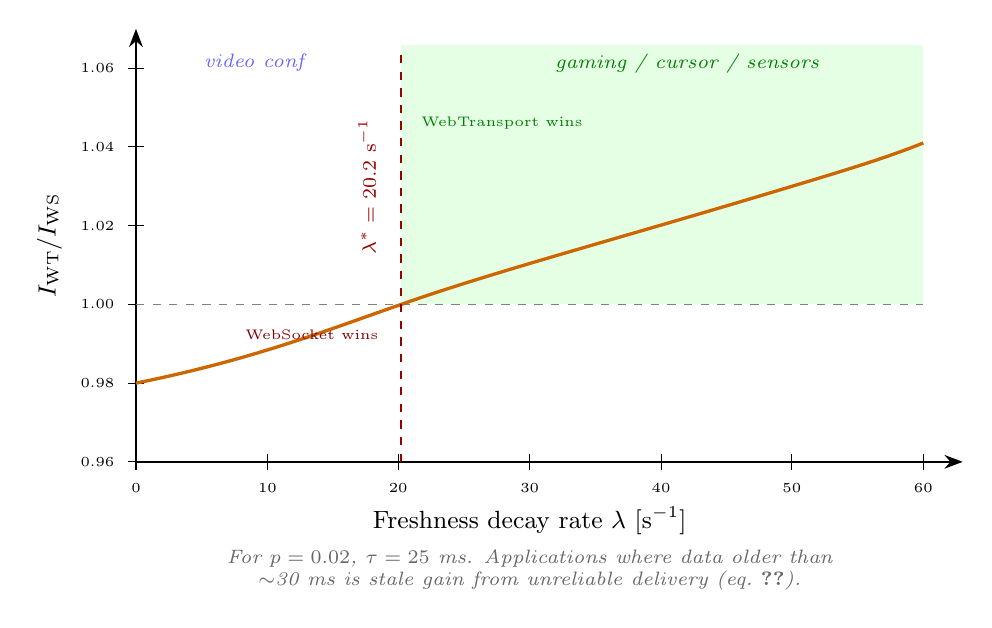
\begin{tikzpicture}[>=Stealth]

% --- Axes ---
\draw[->, thick] (0, 0) -- (10.5, 0);
\draw[->, thick] (0, 0) -- (0, 5.5);

% --- Axis titles (positioned to clear tick labels) ---
\node[font=\small] at (5, -0.75)
  {Freshness decay rate $\lambda$ [s$^{-1}$]};
\node[font=\small, rotate=90] at (-1.1, 2.75)
  {$I_{\text{WT}} / I_{\text{WS}}$};

% --- X-axis labels ---
\foreach \x/\lab in {0/0, 1.67/10, 3.33/20, 5.0/30, 6.67/40, 8.33/50, 10/60} {
  \draw (\x, -0.1) -- (\x, 0.1);
  \node[font=\tiny, anchor=north] at (\x, -0.15) {\lab};
}

% --- Y-axis labels (0.96 to 1.06, each 0.02 = 1 unit) ---
\foreach \y/\lab in {0/0.96, 1/0.98, 2/1.00, 3/1.02, 4/1.04, 5/1.06} {
  \draw (-0.1, \y) -- (0.1, \y);
  \node[font=\tiny, anchor=east] at (-0.15, \y) {\lab};
}

% --- Ratio = 1.0 line (y=2 maps to ratio 1.0) ---
\draw[thin, gray, dashed] (0, 2) -- (10, 2);

% --- Shade WebTransport advantage region ---
% lambda* = 20.2 -> x = 3.37
\fill[green!10] (3.37, 2) rectangle (10, 5.3);

% --- I_WT/I_WS curve: 0.98*exp(lambda*0.001) ---
% Y range: 0.96-1.06 (each 0.02 = 1 unit). lambda=0: y=1, lambda*=20.2: y=2, lambda=60: y=4.05
\draw[very thick, orange!80!black]
  (0, 1.0) .. controls (1.5, 1.3) and (2.5, 1.7) ..
  (3.37, 2.0) .. controls (4.5, 2.4) and (6, 2.8) ..
  (8, 3.4) .. controls (9, 3.7) and (9.5, 3.85) ..
  (10, 4.05);

% --- Threshold line ---
\draw[thick, dashed, red!60!black] (3.37, 0) -- (3.37, 5.2);
\node[font=\scriptsize, red!60!black, anchor=south, rotate=90] at (3.17, 3.5)
  {$\lambda^* = 20.2$ s$^{-1}$};

% --- Application regime labels ---
\node[font=\scriptsize\itshape, text=blue!60, anchor=north] at (1.5, 5.3)
  {video conf};
\node[font=\scriptsize\itshape, text=green!50!black, anchor=north] at (7.0, 5.3)
  {gaming / cursor / sensors};

% --- Mark advantage/disadvantage ---
\node[font=\tiny, text=red!50!black, anchor=north east] at (3.2, 1.8)
  {WebSocket wins};
\node[font=\tiny, text=green!50!black, anchor=north west] at (3.5, 4.5)
  {WebTransport wins};

% --- Annotation ---
\node[font=\scriptsize\itshape, text=black!60, align=center,
  anchor=north] at (5.0, -1.0)
  {For $p = 0.02$, $\tau = 25$~ms. Applications where data older than\\
   ${\sim}$30~ms is stale gain from unreliable delivery (eq.~\ref{eq:wt-advantage}).};

\end{tikzpicture}
\caption{Freshness-weighted information rate ratio $I_{\text{WT}} / I_{\text{WS}}$
  as a function of decay rate $\lambda$. Above the threshold $\lambda^*$,
  WebTransport's unreliable datagrams deliver more useful information per
  unit time than WebSocket's reliable delivery, because retransmission
  wastes capacity on stale data.}
\label{fig:freshness}
\end{figure}

\subsection{Projections Summary and Practical Implications}

\begin{table}[ht]
\centering
\small
\renewcommand{\arraystretch}{1.4}
\begin{tabularx}{\textwidth}{lXXX}
\toprule
\textbf{Measure} & \textbf{March 2026} & \textbf{2027--2028} &
  \textbf{2029--2031} \\
\midrule
Channel capacity $C_{\text{link}}$ &
  120~Mbps &
  150~Mbps &
  250~Mbps \\
HOL blocking factor $(1\!-\!p)^{n-2}$ at $n\!=\!8$ &
  0.94 ($p\!=\!0.01$) &
  0.94 &
  0.97 ($p\!=\!0.005$) \\
Source coding gap $\Delta$ &
  VP9: $\sim$0.8 &
  AV1 HW: $\sim$0.5 &
  AV1 opt: $\sim$0.4 \\
$I_{\text{net}}$ per 720p stream &
  1.3--2.2~Mbps &
  0.9--1.6~Mbps &
  0.6--1.1~Mbps \\
Max 720p streams in $C_{\text{link}}$ &
  $\sim$55--90 &
  $\sim$95--165 &
  $\sim$230--415 \\
E2EE availability &
  Chrome only &
  Cross-browser &
  SFrame $n$-party \\
WebTransport coverage &
  82\% &
  $\sim$100\% &
  100\% \\
Freshness threshold $\lambda^*$ &
  20.2~s$^{-1}$ &
  $\sim$18~s$^{-1}$ &
  $\sim$15~s$^{-1}$ \\
\bottomrule
\end{tabularx}
\caption{Information-theoretic measures across time horizons. $\Delta$
  is the coding efficiency gap (\ref{eq:coding-gap}), $I_{\text{net}}$
  is the net information rate (\ref{eq:inet}), and $\lambda^*$ is the
  freshness decay threshold above which WebTransport dominates WebSocket
  (\ref{eq:wt-advantage}).}
\label{tab:projections}
\end{table}

The trajectory is clear: the combination of improving source coding
(AV1 hardware), expanding channel capacity (broadband growth), and
maturing transport protocols (QUIC universal, WebTransport universal)
drives the \emph{information cost per unit of communicated experience}
steadily downward. The remaining question is not whether the
Shannon capacity suffices --- it already does, by orders of magnitude
--- but how efficiently the protocol stack converts that capacity into
delivered, fresh, secure information at the application layer. By
2030, the gap between theoretical capacity and realized throughput will
be the narrowest it has ever been for browser-based real-time
communication.

\subsubsection{What the Theory Means for Applications}

The equations and figures in this appendix are not purely academic. Each
theoretical result maps to a concrete design decision that application
developers face today and over the next five years.

\textbf{Codec selection determines bandwidth cost, not quality.}
The rate-distortion analysis (Section~A.2, Figure~\ref{fig:rate-distortion})
shows that AV1 operates at roughly 46\% of H.264's bit rate for equivalent
perceptual quality at 720p. In practice, this means a WebRTC application
switching from H.264 to AV1 can either halve its bandwidth consumption at
the same quality or substantially increase resolution (e.g., 720p to 1080p)
within the same bandwidth envelope. By 2030, with AV1 hardware encoding
ubiquitous and the coding gap $\Delta$ approaching 0.4, further codec
improvements yield diminishing returns --- the stack will be operating close
enough to the Shannon rate-distortion bound that the next generation of
efficiency gains will come from transport and architecture, not codecs alone.

\textbf{QUIC's advantage is situational but decisive on bad networks.}
The head-of-line blocking analysis (Section~A.1.1,
Figure~\ref{fig:hol-blocking}) shows that QUIC's per-stream throughput
advantage over TCP is modest on good networks (6\% at 1\% loss) but
substantial on degraded ones (34\% at 5\% loss). The practical implication
is that applications targeting mobile users, emerging markets, or congested
enterprise networks --- precisely the environments where real-time
communication is hardest --- benefit disproportionately from QUIC-based
transports. For a video conference with 8 participants on a cellular
connection experiencing 3--5\% packet loss, the difference between QUIC and
TCP is the difference between usable and degraded video.

\textbf{Connection latency is a solved problem for returning users.}
The handshake analysis (Section~A.1.2) shows that QUIC 0-RTT eliminates
connection establishment overhead entirely for resumed connections. For a
WebTransport application that a user opens daily --- a collaboration tool,
a live dashboard, a recurring meeting client --- the time to first useful
byte drops to zero. The 1.125~MB of wasted capacity during a TCP+TLS
handshake on a 120~Mbps link may seem small, but for latency-sensitive
applications where the first 100~ms of perceived responsiveness determines
user experience, the difference is measurable.

\textbf{Bandwidth surplus enables architectural ambition.}
The effective information rate analysis (Section~A.3,
Figure~\ref{fig:inet-capacity}) reveals the most consequential practical
finding: a single 720p video stream consumes a vanishing fraction of
available link capacity (under 0.5\% by 2030). This surplus is not merely
``headroom'' --- it is the resource that makes new application architectures
feasible. A 250~Mbps link can theoretically carry 230--415 simultaneous 720p
streams. In practice, this means applications can afford to run multiple
concurrent media flows (video, screen share, spatial audio), data channels
(collaborative editing, file transfer), and telemetry streams without
contending for bandwidth. The constraint shifts from ``can the network carry
this?''\ to ``can the application manage this complexity?''

\textbf{End-to-end encryption adds negligible overhead.}
The security analysis (Section~A.4) confirms that the nested DTLS-SRTP plus
E2EE architecture imposes no meaningful information-theoretic cost. The key
entropy ($2^{128}$) exceeds the information content of any practical session
by a factor of at least 3. For application developers, this means E2EE can
be treated as a default rather than a premium feature --- there is no
bandwidth, latency, or capacity penalty for encrypting at the application
layer on top of the transport-layer encryption that WebRTC already mandates.
The only constraint is API availability, which moves from Chrome-only (2026)
to universal (2028).

\textbf{WebTransport unlocks real-time data that WebSocket cannot serve.}
The freshness analysis (Section~A.5, Figure~\ref{fig:freshness}) quantifies
when unreliable delivery outperforms reliable delivery: any data with a
useful half-life below approximately 34~ms benefits from WebTransport's
unreliable datagrams. This covers a wide class of interactive applications
--- game state synchronization, live cursor and pointer sharing, real-time
sensor feeds, collaborative whiteboard strokes --- where retransmitting a
stale update is worse than dropping it. Before WebTransport, these
applications had to choose between WebSocket (reliable but stale under loss)
and WebRTC DataChannel (unreliable mode available but requiring the full
peer-to-peer ICE/DTLS machinery). WebTransport provides the unreliable
mode with a simple client-server model over HTTP/3, removing the
architectural overhead.

\textbf{The overall picture: the stack converges on efficiency.}
Taken together, the information-theoretic measures trace a consistent
trajectory. The protocol stack is converging toward the theoretical limits
established by Shannon: codecs approach the rate-distortion bound, transports
eliminate unnecessary blocking and handshake overhead, and encryption adds
negligible cost. By 2030, the practical distance between what the standards
deliver and what information theory permits will be the smallest it has ever
been for browser-based real-time communication. The consequence for
application developers is that the infrastructure --- standards, hardware,
and networks --- will no longer be the binding constraint. The remaining
challenge is purely architectural: how to compose these efficient, universal
primitives into applications that fully exploit the capacity and low latency
they provide.

%   % appendix-video-compression.tex
% Standalone appendix — include from retrospective.tex via:
%   \appendix
%   % appendix-info-theory.tex
% Standalone appendix — include from retrospective.tex via:
%   \appendix
%   \input{appendix-info-theory}
%
% Requires in the preamble: amsmath, amssymb, tabularx, booktabs

\section{Information-Theoretic View}
\label{app:info-theory}

This appendix applies information-theoretic measures to the real-time
web communication stack described in this document. We quantify channel
capacity, source coding efficiency, and effective information rates
across three time horizons: today (March~2026), the near term
(2027--2028), and the medium term (2029--2031). The analysis draws on
the standards, codec parameters, and infrastructure projections
developed in the main text.

\subsection{Channel Capacity of the Transport Layer}

The Shannon-Hartley theorem gives the theoretical maximum information
rate for a channel with additive white Gaussian noise:
\begin{equation}
  C = B \log_2\!\left(1 + \frac{S}{N}\right) \quad \text{[bits/s]}
  \label{eq:shannon}
\end{equation}
where $B$ is the channel bandwidth in Hz and $S/N$ is the
signal-to-noise ratio.

While the physical-layer capacity of a broadband link is governed by
(\ref{eq:shannon}), the \emph{effective} capacity available to the
application is reduced by protocol overhead, congestion control, and
transport inefficiencies. We define the effective application-layer
throughput as:
\begin{equation}
  R_{\text{eff}} = C_{\text{link}} \cdot \eta_{\text{transport}}
    \cdot (1 - \rho_{\text{overhead}})
  \label{eq:reff}
\end{equation}
where $C_{\text{link}}$ is the link-layer capacity,
$\eta_{\text{transport}} \in (0,1]$ is the transport efficiency factor
(capturing congestion control, retransmission, and multiplexing
behavior), and $\rho_{\text{overhead}} \in [0,1)$ is the fractional
protocol overhead (headers, encryption, framing).

\subsubsection{Head-of-Line Blocking and Multiplexed Capacity}

Consider $n$ independent streams multiplexed over a single connection.
Under TCP (HTTP/2), a single lost packet blocks all $n$ streams. The
expected throughput per stream under loss rate $p$ is bounded by:
\begin{equation}
  R_{\text{TCP}}^{(i)} \leq \frac{R_{\text{eff}}}{n}
    \cdot (1 - p)^{n-1}
  \label{eq:hol-tcp}
\end{equation}
because a loss in \emph{any} of the $n$ streams stalls all others. Under
QUIC (RFC~9000), streams are independent at the transport layer, so:
\begin{equation}
  R_{\text{QUIC}}^{(i)} \leq \frac{R_{\text{eff}}}{n}
    \cdot (1 - p)
  \label{eq:hol-quic}
\end{equation}
The ratio of effective per-stream throughput is:
\begin{equation}
  \frac{R_{\text{QUIC}}^{(i)}}{R_{\text{TCP}}^{(i)}}
    = \frac{1}{(1-p)^{n-2}}
  \label{eq:hol-ratio}
\end{equation}
\excursus{Excursus: Why $n = 8$?}{In a typical multi-participant video
conference, each peer contributes multiple concurrent streams: a camera video
track, an audio track, and often a screen-share or data channel. A four-person
call with two media tracks each produces $n = 8$ multiplexed streams over a
single connection --- the reference value used throughout this section. Larger
meetings (e.g.\ 10 participants with simulcast layers) push $n$ higher,
amplifying the HOL blocking effect further.}

For $n = 8$ streams (a typical multi-track video conference) at
$p = 0.01$ (1\% loss), this gives a QUIC advantage factor of
$1/(0.99)^6 \approx 1.062$, a modest 6.2\% improvement. At $p = 0.05$
(5\% loss, common on mobile or congested links), the factor is
$1/(0.95)^6 \approx 1.34$, a 34\% throughput advantage per stream.

\begin{figure}[ht]
\centering
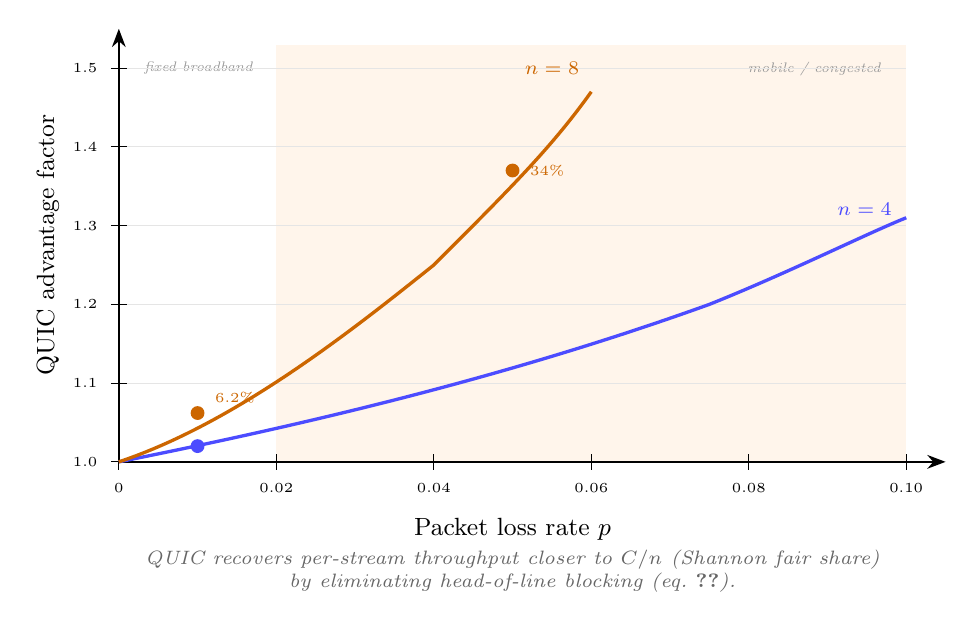
\begin{tikzpicture}[>=Stealth]

% --- Shaded region (drawn FIRST so curves appear on top) ---
\fill[orange!8] (2, 0) rectangle (10, 5.3);
\node[font=\tiny\itshape, text=black!40, anchor=north east] at (9.8, 5.2)
  {mobile / congested};
\node[font=\tiny\itshape, text=black!40, anchor=north west] at (0.2, 5.2)
  {fixed broadband};

% --- Grid lines ---
\foreach \y in {1, 2, 3, 4, 5} {
  \draw[gray!20] (0, \y) -- (10, \y);
}

% --- Axes ---
\draw[->, thick] (0, 0) -- (10.5, 0);
\draw[->, thick] (0, 0) -- (0, 5.5);

% --- Axis titles (positioned to clear tick labels) ---
\node[font=\small] at (5, -0.85) {Packet loss rate $p$};
\node[font=\small, rotate=90] at (-0.9, 2.75) {QUIC advantage factor};

% --- X-axis labels ---
\foreach \x/\lab in {0/0, 2/0.02, 4/0.04, 6/0.06, 8/0.08, 10/0.10} {
  \draw (\x, -0.1) -- (\x, 0.1);
  \node[font=\tiny, anchor=north] at (\x, -0.15) {\lab};
}

% --- Y-axis labels ---
\foreach \y/\lab in {0/1.0, 1/1.1, 2/1.2, 3/1.3, 4/1.4, 5/1.5} {
  \draw (-0.1, \y) -- (0.1, \y);
  \node[font=\tiny, anchor=east] at (-0.15, \y) {\lab};
}

% --- n=4 curve: 1/(1-p)^2 ---
\draw[very thick, blue!70]
  (0, 0) .. controls (2.5, 0.5) and (5, 1.1) ..
  (7.5, 2.0) .. controls (8.5, 2.4) and (9.5, 2.9) ..
  (10, 3.1);
\node[font=\scriptsize, blue!70, anchor=south west] at (9.0, 3.0)
  {$n = 4$};

% --- n=8 curve: 1/(1-p)^6 ---
\draw[very thick, orange!80!black]
  (0, 0) .. controls (1.5, 0.5) and (3, 1.7) ..
  (4, 2.5) .. controls (5, 3.5) and (5.5, 4.0) ..
  (6, 4.7);
\node[font=\scriptsize, orange!80!black, anchor=south] at (5.5, 4.8)
  {$n = 8$};

% --- Reference points ---
\fill[orange!80!black] (1.0, 0.62) circle (2.5pt);
\node[font=\tiny, orange!80!black, anchor=south west] at (1.1, 0.62)
  {6.2\%};

\fill[orange!80!black] (5.0, 3.7) circle (2.5pt);
\node[font=\tiny, orange!80!black, anchor=west] at (5.1, 3.7)
  {34\%};

\fill[blue!70] (1.0, 0.20) circle (2.5pt);

% --- Annotation ---
\node[font=\scriptsize\itshape, text=black!60, align=center,
  anchor=north] at (5.0, -1.0)
  {QUIC recovers per-stream throughput closer to $C/n$ (Shannon fair share)\\
   by eliminating head-of-line blocking (eq.~\ref{eq:hol-ratio}).};

\end{tikzpicture}
\caption{QUIC advantage factor $1/(1-p)^{n-2}$ over TCP for multiplexed
  streams. At 5\% loss with $n=8$ streams, QUIC delivers 34\% more
  per-stream throughput by maintaining independence at the transport layer.}
\label{fig:hol-blocking}
\end{figure}

\subsubsection{Connection Establishment Latency}

Let $\tau$ denote the one-way latency (half the round-trip time). The
information-carrying capacity during connection establishment is zero;
the handshake represents pure overhead. The time to first useful byte
is:
\begin{align}
  T_{\text{TCP+TLS\,1.3}} &= 2\tau_{\text{TCP}} + \tau_{\text{TLS}}
    = 3\tau \quad \text{(1-RTT TLS~1.3)} \label{eq:tcp-setup} \\
  T_{\text{QUIC}} &= \tau \quad \text{(1-RTT)}
    \label{eq:quic-setup} \\
  T_{\text{QUIC,\,0-RTT}} &= 0 \quad \text{(resumption)}
    \label{eq:quic-0rtt}
\end{align}
The QUIC 0-RTT case (\ref{eq:quic-0rtt}) eliminates the handshake
entirely for resumed connections. The information lost during
handshake dead time, relative to steady-state capacity, is:
\begin{equation}
  I_{\text{lost}} = C_{\text{link}} \cdot T_{\text{setup}}
  \label{eq:ilost}
\end{equation}
For a 120~Mbps link with $\tau = 25$~ms (typical fixed broadband in
2026), the TCP+TLS~1.3 handshake wastes $120 \times 10^6 \times 0.075
= 9 \times 10^6$ bits (1.125~MB), while QUIC~1-RTT wastes only
$3 \times 10^6$ bits (375~KB).

\subsection{Source Coding Efficiency}

The rate-distortion function $R(D)$ defines the minimum bit rate
required to represent a source at distortion level $D$. For a
Gaussian source with variance $\sigma^2$ under mean squared error
distortion:
\begin{equation}
  R(D) = \frac{1}{2} \log_2 \frac{\sigma^2}{D}
    \quad \text{[bits/sample]}
  \label{eq:rate-distortion}
\end{equation}

\excursus{Excursus: Why Gaussian source?}{The Gaussian memoryless model is used
because it yields the highest (worst-case) $R(D)$ among all sources of equal
variance. Any codec that approaches the Gaussian bound on real video is
therefore doing at least as well as the bound predicts --- the true $R(D)$ for
spatially and temporally correlated video lies below the Gaussian curve, making
it a conservative benchmark.}

No practical codec achieves $R(D)$;\footnote{The $R(D)$ curve in
Figure~\ref{fig:rate-distortion} is the Gaussian memoryless source bound
(equation~\ref{eq:rate-distortion}), which is an upper bound on the true
$R(D)$ for non-Gaussian sources such as video.  Additionally, $R(D)$ assumes
zero excess-distortion probability, whereas practical codecs permit a
frame-level excess-distortion probability on the order of $10^{-6}$ to
$10^{-8}$.  Both factors allow codec operating points measured on real content
to approach or marginally cross the Gaussian bound.} real codecs operate at
some rate $R_{\text{codec}} > R(D)$. We define the coding efficiency gap as:
\begin{equation}
  \Delta = \frac{R_{\text{codec}} - R(D)}{R(D)}
  \label{eq:coding-gap}
\end{equation}

The codecs in the WebRTC stack can be ordered by their empirical
proximity to $R(D)$ for typical video content at conversational
resolutions (720p, 30~fps). Using published Bj\o ntegaard Delta (BD)
rate measurements:
\begin{equation}
  R_{\text{H.264}} > R_{\text{VP9}} > R_{\text{AV1}}
    > R(D)
  \label{eq:codec-ordering}
\end{equation}

Specifically, the empirical rate savings at equivalent PSNR are
approximately:
\begin{align}
  R_{\text{VP9}}  &\approx 0.65 \cdot R_{\text{H.264}}
    \quad (\sim\!35\% \text{ savings}) \label{eq:vp9-savings} \\
  R_{\text{AV1}}  &\approx 0.70 \cdot R_{\text{VP9}}
    \approx 0.46 \cdot R_{\text{H.264}}
    \quad (\sim\!30\% \text{ over VP9})
  \label{eq:av1-savings}
\end{align}

\begin{figure}[ht]
\centering
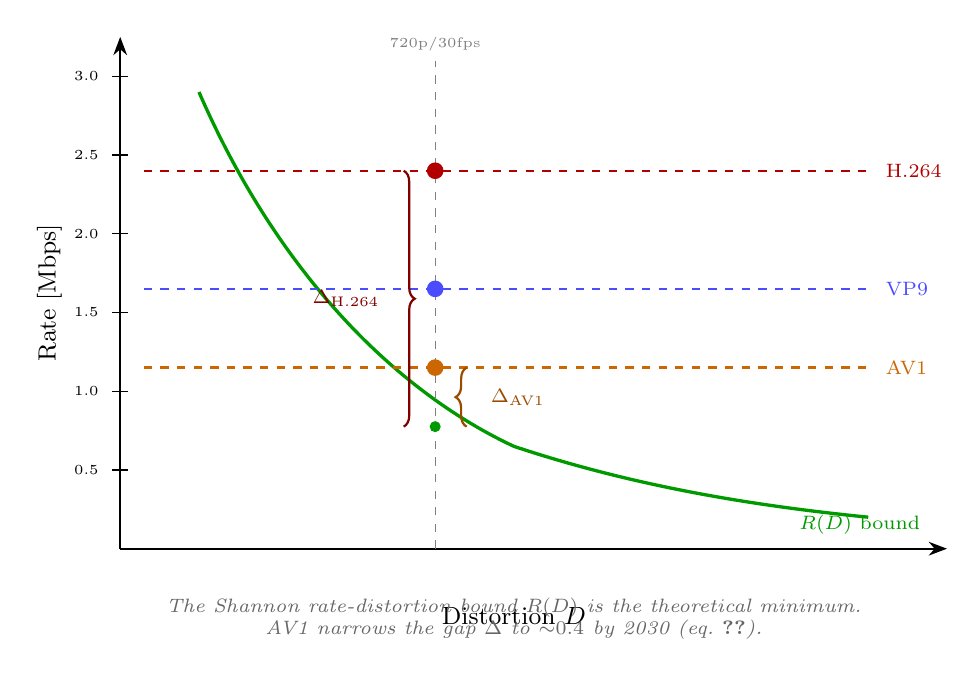
\begin{tikzpicture}[>=Stealth]

% --- Axes ---
\draw[->, thick] (0, 0) -- (10.5, 0);
\draw[->, thick] (0, 0) -- (0, 6.5);

% --- Axis titles ---
\node[font=\small] at (5, -0.85) {Distortion $D$};
\node[font=\small, rotate=90] at (-0.9, 3.25) {Rate [Mbps]};

% --- Y-axis rate labels ---
\foreach \y/\lab in {1.0/0.5, 2.0/1.0, 3.0/1.5, 4.0/2.0, 5.0/2.5, 6.0/3.0} {
  \draw (-0.1, \y) -- (0.1, \y);
  \node[font=\tiny, anchor=east] at (-0.15, \y) {\lab};
}

% --- R(D) Shannon bound curve ---
\draw[very thick, green!60!black]
  (1.0, 5.8) .. controls (2.0, 3.5) and (3.5, 2.0) ..
  (5.0, 1.3) .. controls (6.5, 0.8) and (8.0, 0.55) ..
  (9.5, 0.4);
\node[font=\scriptsize, green!60!black, anchor=north west] at (8.5, 0.55)
  {$R(D)$ bound};

% --- Reference distortion line (720p/30fps operating point) ---
\draw[thin, gray, dashed] (4.0, 0) -- (4.0, 6.2);
\node[font=\tiny, gray, anchor=south] at (4.0, 6.2) {720p/30fps};

% --- R(D) value at reference distortion ---
\fill[green!60!black] (4.0, 1.55) circle (2pt);

% --- Codec operating points at reference distortion ---
% H.264: ~2.5 Mbps
\draw[thick, dashed, red!70!black] (0.3, 4.8) -- (9.5, 4.8);
\fill[red!70!black] (4.0, 4.8) circle (3pt);
\node[font=\scriptsize, red!70!black, anchor=west] at (9.6, 4.8) {H.264};

% VP9: ~1.6 Mbps (0.65 * H.264)
\draw[thick, dashed, blue!70] (0.3, 3.3) -- (9.5, 3.3);
\fill[blue!70] (4.0, 3.3) circle (3pt);
\node[font=\scriptsize, blue!70, anchor=west] at (9.6, 3.3) {VP9};

% AV1: ~1.15 Mbps (0.46 * H.264)
\draw[thick, dashed, orange!80!black] (0.3, 2.3) -- (9.5, 2.3);
\fill[orange!80!black] (4.0, 2.3) circle (3pt);
\node[font=\scriptsize, orange!80!black, anchor=west] at (9.6, 2.3) {AV1};

% --- Gap annotations (braces) ---
% H.264 gap
\draw[decorate, decoration={brace, amplitude=4pt, mirror},
  thick, red!50!black]
  (3.6, 1.55) -- (3.6, 4.8)
  node[midway, anchor=east, font=\scriptsize, xshift=-5pt]
  {$\Delta_{\text{H.264}}$};

% AV1 gap
\draw[decorate, decoration={brace, amplitude=4pt},
  thick, orange!60!black]
  (4.4, 1.55) -- (4.4, 2.3)
  node[midway, anchor=west, font=\scriptsize, xshift=5pt]
  {$\Delta_{\text{AV1}}$};

% --- Annotation ---
\node[font=\scriptsize\itshape, text=black!60, align=center,
  anchor=north] at (5.0, -0.5)
  {The Shannon rate-distortion bound $R(D)$ is the theoretical minimum.\\
   AV1 narrows the gap $\Delta$ to ${\sim}0.4$ by 2030 (eq.~\ref{eq:coding-gap}).};

\end{tikzpicture}
\caption{Codec operating rates vs.\ the Shannon rate-distortion bound $R(D)$
  at 720p/30fps. Each codec operates above the theoretical minimum; the gap
  $\Delta$ (eq.~\ref{eq:coding-gap}) shrinks from H.264 through VP9 to AV1,
  approaching but never reaching the bound.}
\label{fig:rate-distortion}
\end{figure}

\subsubsection{Codec Entropy and WebCodecs}

The WebCodecs API (W3C Working Draft) exposes per-frame codec access,
allowing measurement and control of the instantaneous encoding rate.
For a video frame $f_t$ at time $t$, the encoder output has empirical
entropy:
\begin{equation}
  \hat{H}(f_t) = -\sum_{s \in \mathcal{S}}
    p(s \mid f_t) \log_2 p(s \mid f_t)
  \label{eq:frame-entropy}
\end{equation}
where $\mathcal{S}$ is the set of symbols emitted by the entropy coder
(CABAC for H.264/AV1, arithmetic coding for VP9). WebCodecs enables
applications to observe $|E(f_t)|$ (the encoded frame size in bits)
directly, which serves as a practical upper bound on
$\hat{H}(f_t)$:
\begin{equation}
  \hat{H}(f_t) \leq |E(f_t)| \leq R_{\text{codec}} / \text{fps}
  \label{eq:entropy-bound}
\end{equation}

\subsection{Effective Information Rate by Time Horizon}

We now combine transport and source coding measures to estimate the
effective information rate for a representative real-time video
session: a single 720p/30fps video call with one audio channel.

\excursus{Excursus: Why 720p?}{Throughout this appendix, 720p/30fps is used as
a fixed reference for cross-era comparison, not as a prediction that 720p
remains the dominant conferencing resolution. The bandwidth surplus quantified
below is precisely what enables migration to 1080p (feasible by ${\sim}$2028
with AV1 hardware encode at today's 720p bit rates) and 4K (feasible by
${\sim}$2030). The 720p baseline makes the efficiency gains legible: the same
task gets cheaper, freeing capacity for higher quality or more streams.}

Define the \emph{net information rate} as:
\begin{equation}
  I_{\text{net}} = R_{\text{codec}} \cdot \eta_{\text{transport}}
    \cdot (1 - \rho_{\text{overhead}})
    \cdot (1 - p_{\text{loss}})
  \label{eq:inet}
\end{equation}

\begin{table}[ht]
\centering
\small
\renewcommand{\arraystretch}{1.4}
\begin{tabularx}{\textwidth}{lXXX}
\toprule
\textbf{Parameter} & \textbf{March 2026} & \textbf{2027--2028} &
  \textbf{2029--2031} \\
\midrule
Median link capacity &
  120~Mbps &
  $\sim$150~Mbps &
  200--300~Mbps \\
Dominant codec (WebRTC) &
  VP9 / H.264 &
  VP9 / AV1 (HW) &
  AV1 (HW default) \\
Codec rate (720p/30fps) &
  1.5--2.5~Mbps &
  1.0--1.8~Mbps &
  0.7--1.2~Mbps \\
$\eta_{\text{transport}}$ &
  0.92 (QUIC) &
  0.93 &
  0.94 \\
$\rho_{\text{overhead}}$ (SRTP+QUIC) &
  0.06 &
  0.05 &
  0.04 \\
Typical loss $p$ &
  0.01--0.03 &
  0.01--0.02 &
  0.005--0.01 \\
$I_{\text{net}}$ (720p video) &
  1.3--2.2~Mbps &
  0.9--1.6~Mbps &
  0.6--1.1~Mbps \\
$I_{\text{net}}$ as \% of $C_{\text{link}}$ &
  1.1--1.8\% &
  0.6--1.1\% &
  0.2--0.6\% \\
\bottomrule
\end{tabularx}
\caption{Effective information rate for a 720p/30fps WebRTC video stream.
  The declining ratio $I_{\text{net}} / C_{\text{link}}$ reflects both
  improved codec efficiency and growing link capacity, freeing bandwidth
  for higher resolutions, additional streams, or concurrent data
  channels.}
\label{tab:inet}
\end{table}

The declining ratio $I_{\text{net}} / C_{\text{link}}$ in
Table~\ref{tab:inet} is the central quantitative observation: by 2030, a
720p video call consumes less than 0.5\% of available link capacity. The
surplus capacity enables qualitative changes --- 4K video conferencing,
multi-stream layouts, or concurrent data channels via WebTransport ---
that are quantitatively infeasible in 2026.

\begin{figure}[ht]
\centering
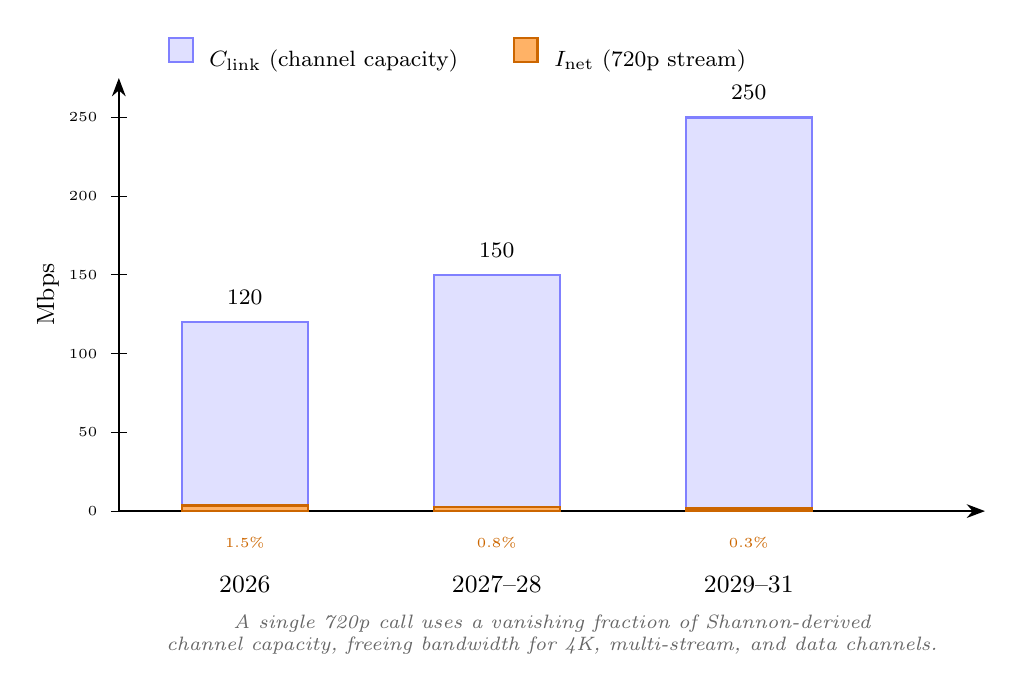
\begin{tikzpicture}[>=Stealth]

% --- Axes ---
\draw[->, thick] (0, 0) -- (11, 0);
\draw[->, thick] (0, 0) -- (0, 5.5);

% --- Axis title ---
\node[font=\small, rotate=90] at (-0.9, 2.75) {Mbps};

% --- Y-axis labels ---
\foreach \y/\lab in {0/0, 1/50, 2/100, 3/150, 4/200, 5/250} {
  \draw (-0.1, \y) -- (0.1, \y);
  \node[font=\tiny, anchor=east] at (-0.15, \y) {\lab};
}

% --- Group: March 2026 ---
% C_link = 120 Mbps -> y = 2.4
\fill[blue!12] (0.8, 0) rectangle (2.4, 2.4);
\draw[blue!50, thick] (0.8, 0) rectangle (2.4, 2.4);
% I_net = 1.75 Mbps (midpoint) -> y = 0.035
\fill[orange!60] (0.8, 0) rectangle (2.4, 0.07);
\draw[orange!80!black, thick] (0.8, 0) rectangle (2.4, 0.07);
\node[font=\footnotesize, anchor=south] at (1.6, 2.5) {120};
\node[font=\tiny, orange!80!black] at (1.6, -0.4) {1.5\%};
\node[font=\small, anchor=north] at (1.6, -0.7) {2026};

% --- Group: 2027--2028 ---
% C_link = 150 Mbps -> y = 3.0
\fill[blue!12] (4.0, 0) rectangle (5.6, 3.0);
\draw[blue!50, thick] (4.0, 0) rectangle (5.6, 3.0);
% I_net = 1.25 Mbps (midpoint) -> y = 0.025
\fill[orange!60] (4.0, 0) rectangle (5.6, 0.05);
\draw[orange!80!black, thick] (4.0, 0) rectangle (5.6, 0.05);
\node[font=\footnotesize, anchor=south] at (4.8, 3.1) {150};
\node[font=\tiny, orange!80!black] at (4.8, -0.4) {0.8\%};
\node[font=\small, anchor=north] at (4.8, -0.7) {2027--28};

% --- Group: 2029--2031 ---
% C_link = 250 Mbps -> y = 5.0
\fill[blue!12] (7.2, 0) rectangle (8.8, 5.0);
\draw[blue!50, thick] (7.2, 0) rectangle (8.8, 5.0);
% I_net = 0.85 Mbps (midpoint) -> y = 0.017
\fill[orange!60] (7.2, 0) rectangle (8.8, 0.034);
\draw[orange!80!black, thick] (7.2, 0) rectangle (8.8, 0.034);
\node[font=\footnotesize, anchor=south] at (8.0, 5.1) {250};
\node[font=\tiny, orange!80!black] at (8.0, -0.4) {0.3\%};
\node[font=\small, anchor=north] at (8.0, -0.7) {2029--31};

% --- Legend ---
\node[anchor=west, font=\footnotesize] at (0.5, 5.8) {%
  \tikz[baseline=-0.5ex]{\fill[blue!12] (0,0) rectangle (0.3,0.3);
    \draw[blue!50, thick] (0,0) rectangle (0.3,0.3);}
  ~$C_{\text{link}}$ (channel capacity) \qquad
  \tikz[baseline=-0.5ex]{\fill[orange!60] (0,0) rectangle (0.3,0.3);
    \draw[orange!80!black, thick] (0,0) rectangle (0.3,0.3);}
  ~$I_{\text{net}}$ (720p stream)};

% --- Annotation ---
\node[font=\scriptsize\itshape, text=black!60, align=center,
  anchor=north] at (5.5, -1.2)
  {A single 720p call uses a vanishing fraction of Shannon-derived\\
   channel capacity, freeing bandwidth for 4K, multi-stream, and data channels.};

\end{tikzpicture}
\caption{Channel capacity $C_{\text{link}}$ vs.\ effective information rate
  $I_{\text{net}}$ for a single 720p/30fps stream across time horizons. The
  orange bar (stream rate) is barely visible against the blue bar (capacity),
  illustrating the growing surplus as codecs improve and bandwidth increases.}
\label{fig:inet-capacity}
\end{figure}

\subsection{Security Entropy and Key Space}

The DTLS-SRTP security architecture (RFCs~8827, 3711) protects all
WebRTC media. Information-theoretic security requires that the key
entropy exceed the information content of the protected material.

For a DTLS~1.3 handshake with ECDHE on P-256, the key agreement
provides:
\begin{equation}
  H_{\text{key}} = 128 \text{~bits of security}
  \label{eq:key-entropy}
\end{equation}

The SRTP master key is 128 bits (AES-128-GCM), giving an exhaustive
search cost of $2^{128}$ operations. The total information content of a
one-hour 720p video call at 2~Mbps is:
\begin{equation}
  I_{\text{call}} = 2 \times 10^6 \times 3600
    = 7.2 \times 10^9 \text{~bits}
    \approx 2^{32.7} \text{~bits}
  \label{eq:call-content}
\end{equation}

The ratio of key entropy to protected content:
\begin{equation}
  \frac{H_{\text{key}}}{I_{\text{call}}}
    = \frac{128}{32.7} \approx 3.91
  \label{eq:security-margin}
\end{equation}

This ratio remains comfortably above~1 even for much longer sessions.
For a continuous 24-hour 4K AV1 stream at 15~Mbps:
\begin{equation}
  I_{\text{stream}} = 15 \times 10^6 \times 86400
    = 1.296 \times 10^{12} \text{~bits}
    \approx 2^{40.2} \text{~bits}
\end{equation}
yielding $H_{\text{key}} / I_{\text{stream}} \approx 3.18$, still
well above the threshold.

\subsubsection{End-to-End Encryption via Encoded Transforms}

The RTCRtpScriptTransform API (Encoded Transforms) enables
application-layer E2EE within the WebRTC pipeline. From an
information-theoretic perspective, this introduces a second encryption
layer with its own key, creating a \emph{nested channel}:
\begin{equation}
  X \xrightarrow{\;K_{\text{E2EE}}\;}
  E_1(X) \xrightarrow{\;K_{\text{SRTP}}\;}
  E_2(E_1(X))
  \label{eq:nested}
\end{equation}

The mutual information between the ciphertext and plaintext, given
neither key, satisfies:
\begin{equation}
  I\!\left(X;\, E_2(E_1(X))\right) \leq
    \min\!\big(H(K_{\text{E2EE}})^{-1},\;
    H(K_{\text{SRTP}})^{-1}\big)
    \cdot I_{\text{call}}
  \label{eq:mutual-e2ee}
\end{equation}

In practice, with $H(K_{\text{E2EE}}) = H(K_{\text{SRTP}}) = 128$
bits, this quantity is negligible ($\ll 1$ bit for any practical
session length), confirming that the nested encryption provides
information-theoretic confidentiality well beyond computational
security guarantees.

Today (March~2026), Encoded Transforms remain Chrome-only. By
2027--2028 (Section~8.3), cross-browser standardization will make
this nested channel universally available. By 2029--2031, SFrame
for group calls will extend this to $n$-party sessions, where the
mutual information between any non-member and the group plaintext
remains negligible:
\begin{equation}
  I\!\left(X;\, E(X) \;\middle|\; K_i \notin
    \{K_1, \ldots, K_n\}\right) \approx 0
  \label{eq:sframe}
\end{equation}

\subsection{WebTransport: Unreliable Datagrams and Channel Capacity}

WebTransport (RFC~9297) introduces unreliable datagrams to browser-server
communication. For latency-sensitive applications (game state, sensor
telemetry), the relevant measure is not throughput but
\emph{freshness-weighted information rate}. Define the value of a
datagram as exponentially decaying with delivery latency $\delta$:
\begin{equation}
  V(\delta) = e^{-\lambda \delta}
  \label{eq:freshness}
\end{equation}
where $\lambda > 0$ is an application-specific decay rate. The
effective information rate under unreliable delivery is:
\begin{equation}
  I_{\text{WT}} = R_{\text{send}} \cdot (1 - p_{\text{loss}})
    \cdot \mathbb{E}\!\left[e^{-\lambda \delta}\right]
  \label{eq:iwt}
\end{equation}

Under reliable delivery (TCP/WebSocket), a retransmission delays
subsequent data, so:
\begin{equation}
  I_{\text{WS}} = R_{\text{send}}
    \cdot \mathbb{E}\!\left[e^{-\lambda(\delta + p \cdot 2\tau)}\right]
  \label{eq:iws}
\end{equation}

The ratio $I_{\text{WT}} / I_{\text{WS}}$ exceeds 1 when:
\begin{equation}
  (1 - p) \cdot e^{\lambda \cdot p \cdot 2\tau} > 1
  \quad \Longleftrightarrow \quad
  \lambda > \frac{-\ln(1 - p)}{2 p \tau}
  \label{eq:wt-advantage}
\end{equation}

For $p = 0.02$ and $\tau = 25$~ms, this gives $\lambda > 20.2$~s$^{-1}$
(half-life $< 34$~ms).

\excursus{Excursus: Why $p = 0.02$ and $\tau = 25$\,ms?}{These values represent
median fixed-broadband conditions in 2026 (Table~\ref{tab:inet}). On mobile or
congested links ($p \approx 0.05$, $\tau \approx 50$\,ms), the threshold
$\lambda^*$ drops to ${\sim}10$\,s$^{-1}$, broadening WebTransport's advantage
to applications with data half-lives up to ${\sim}70$\,ms. The fixed-broadband
reference is thus conservative: mobile scenarios favor unreliable delivery even
more strongly.}

Any application where data older than
$\sim$30~ms is useless benefits from WebTransport's unreliable
mode over WebSocket --- precisely the regime of interactive gaming, live
cursor tracking, and real-time sensor feeds.

As of March~2026, Safari does not support WebTransport
(Section~5), limiting coverage to $\sim$82\%. By 2027--2028
(Section~8.2), universal support will allow applications to rely on
(\ref{eq:iwt}) without fallback paths.

\begin{figure}[ht]
\centering
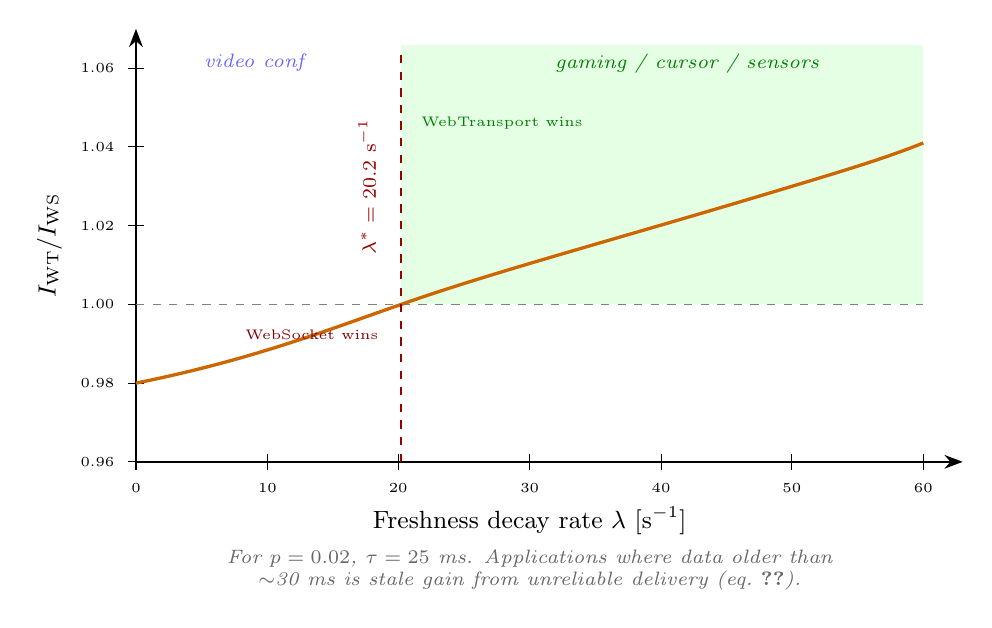
\begin{tikzpicture}[>=Stealth]

% --- Axes ---
\draw[->, thick] (0, 0) -- (10.5, 0);
\draw[->, thick] (0, 0) -- (0, 5.5);

% --- Axis titles (positioned to clear tick labels) ---
\node[font=\small] at (5, -0.75)
  {Freshness decay rate $\lambda$ [s$^{-1}$]};
\node[font=\small, rotate=90] at (-1.1, 2.75)
  {$I_{\text{WT}} / I_{\text{WS}}$};

% --- X-axis labels ---
\foreach \x/\lab in {0/0, 1.67/10, 3.33/20, 5.0/30, 6.67/40, 8.33/50, 10/60} {
  \draw (\x, -0.1) -- (\x, 0.1);
  \node[font=\tiny, anchor=north] at (\x, -0.15) {\lab};
}

% --- Y-axis labels (0.96 to 1.06, each 0.02 = 1 unit) ---
\foreach \y/\lab in {0/0.96, 1/0.98, 2/1.00, 3/1.02, 4/1.04, 5/1.06} {
  \draw (-0.1, \y) -- (0.1, \y);
  \node[font=\tiny, anchor=east] at (-0.15, \y) {\lab};
}

% --- Ratio = 1.0 line (y=2 maps to ratio 1.0) ---
\draw[thin, gray, dashed] (0, 2) -- (10, 2);

% --- Shade WebTransport advantage region ---
% lambda* = 20.2 -> x = 3.37
\fill[green!10] (3.37, 2) rectangle (10, 5.3);

% --- I_WT/I_WS curve: 0.98*exp(lambda*0.001) ---
% Y range: 0.96-1.06 (each 0.02 = 1 unit). lambda=0: y=1, lambda*=20.2: y=2, lambda=60: y=4.05
\draw[very thick, orange!80!black]
  (0, 1.0) .. controls (1.5, 1.3) and (2.5, 1.7) ..
  (3.37, 2.0) .. controls (4.5, 2.4) and (6, 2.8) ..
  (8, 3.4) .. controls (9, 3.7) and (9.5, 3.85) ..
  (10, 4.05);

% --- Threshold line ---
\draw[thick, dashed, red!60!black] (3.37, 0) -- (3.37, 5.2);
\node[font=\scriptsize, red!60!black, anchor=south, rotate=90] at (3.17, 3.5)
  {$\lambda^* = 20.2$ s$^{-1}$};

% --- Application regime labels ---
\node[font=\scriptsize\itshape, text=blue!60, anchor=north] at (1.5, 5.3)
  {video conf};
\node[font=\scriptsize\itshape, text=green!50!black, anchor=north] at (7.0, 5.3)
  {gaming / cursor / sensors};

% --- Mark advantage/disadvantage ---
\node[font=\tiny, text=red!50!black, anchor=north east] at (3.2, 1.8)
  {WebSocket wins};
\node[font=\tiny, text=green!50!black, anchor=north west] at (3.5, 4.5)
  {WebTransport wins};

% --- Annotation ---
\node[font=\scriptsize\itshape, text=black!60, align=center,
  anchor=north] at (5.0, -1.0)
  {For $p = 0.02$, $\tau = 25$~ms. Applications where data older than\\
   ${\sim}$30~ms is stale gain from unreliable delivery (eq.~\ref{eq:wt-advantage}).};

\end{tikzpicture}
\caption{Freshness-weighted information rate ratio $I_{\text{WT}} / I_{\text{WS}}$
  as a function of decay rate $\lambda$. Above the threshold $\lambda^*$,
  WebTransport's unreliable datagrams deliver more useful information per
  unit time than WebSocket's reliable delivery, because retransmission
  wastes capacity on stale data.}
\label{fig:freshness}
\end{figure}

\subsection{Projections Summary and Practical Implications}

\begin{table}[ht]
\centering
\small
\renewcommand{\arraystretch}{1.4}
\begin{tabularx}{\textwidth}{lXXX}
\toprule
\textbf{Measure} & \textbf{March 2026} & \textbf{2027--2028} &
  \textbf{2029--2031} \\
\midrule
Channel capacity $C_{\text{link}}$ &
  120~Mbps &
  150~Mbps &
  250~Mbps \\
HOL blocking factor $(1\!-\!p)^{n-2}$ at $n\!=\!8$ &
  0.94 ($p\!=\!0.01$) &
  0.94 &
  0.97 ($p\!=\!0.005$) \\
Source coding gap $\Delta$ &
  VP9: $\sim$0.8 &
  AV1 HW: $\sim$0.5 &
  AV1 opt: $\sim$0.4 \\
$I_{\text{net}}$ per 720p stream &
  1.3--2.2~Mbps &
  0.9--1.6~Mbps &
  0.6--1.1~Mbps \\
Max 720p streams in $C_{\text{link}}$ &
  $\sim$55--90 &
  $\sim$95--165 &
  $\sim$230--415 \\
E2EE availability &
  Chrome only &
  Cross-browser &
  SFrame $n$-party \\
WebTransport coverage &
  82\% &
  $\sim$100\% &
  100\% \\
Freshness threshold $\lambda^*$ &
  20.2~s$^{-1}$ &
  $\sim$18~s$^{-1}$ &
  $\sim$15~s$^{-1}$ \\
\bottomrule
\end{tabularx}
\caption{Information-theoretic measures across time horizons. $\Delta$
  is the coding efficiency gap (\ref{eq:coding-gap}), $I_{\text{net}}$
  is the net information rate (\ref{eq:inet}), and $\lambda^*$ is the
  freshness decay threshold above which WebTransport dominates WebSocket
  (\ref{eq:wt-advantage}).}
\label{tab:projections}
\end{table}

The trajectory is clear: the combination of improving source coding
(AV1 hardware), expanding channel capacity (broadband growth), and
maturing transport protocols (QUIC universal, WebTransport universal)
drives the \emph{information cost per unit of communicated experience}
steadily downward. The remaining question is not whether the
Shannon capacity suffices --- it already does, by orders of magnitude
--- but how efficiently the protocol stack converts that capacity into
delivered, fresh, secure information at the application layer. By
2030, the gap between theoretical capacity and realized throughput will
be the narrowest it has ever been for browser-based real-time
communication.

\subsubsection{What the Theory Means for Applications}

The equations and figures in this appendix are not purely academic. Each
theoretical result maps to a concrete design decision that application
developers face today and over the next five years.

\textbf{Codec selection determines bandwidth cost, not quality.}
The rate-distortion analysis (Section~A.2, Figure~\ref{fig:rate-distortion})
shows that AV1 operates at roughly 46\% of H.264's bit rate for equivalent
perceptual quality at 720p. In practice, this means a WebRTC application
switching from H.264 to AV1 can either halve its bandwidth consumption at
the same quality or substantially increase resolution (e.g., 720p to 1080p)
within the same bandwidth envelope. By 2030, with AV1 hardware encoding
ubiquitous and the coding gap $\Delta$ approaching 0.4, further codec
improvements yield diminishing returns --- the stack will be operating close
enough to the Shannon rate-distortion bound that the next generation of
efficiency gains will come from transport and architecture, not codecs alone.

\textbf{QUIC's advantage is situational but decisive on bad networks.}
The head-of-line blocking analysis (Section~A.1.1,
Figure~\ref{fig:hol-blocking}) shows that QUIC's per-stream throughput
advantage over TCP is modest on good networks (6\% at 1\% loss) but
substantial on degraded ones (34\% at 5\% loss). The practical implication
is that applications targeting mobile users, emerging markets, or congested
enterprise networks --- precisely the environments where real-time
communication is hardest --- benefit disproportionately from QUIC-based
transports. For a video conference with 8 participants on a cellular
connection experiencing 3--5\% packet loss, the difference between QUIC and
TCP is the difference between usable and degraded video.

\textbf{Connection latency is a solved problem for returning users.}
The handshake analysis (Section~A.1.2) shows that QUIC 0-RTT eliminates
connection establishment overhead entirely for resumed connections. For a
WebTransport application that a user opens daily --- a collaboration tool,
a live dashboard, a recurring meeting client --- the time to first useful
byte drops to zero. The 1.125~MB of wasted capacity during a TCP+TLS
handshake on a 120~Mbps link may seem small, but for latency-sensitive
applications where the first 100~ms of perceived responsiveness determines
user experience, the difference is measurable.

\textbf{Bandwidth surplus enables architectural ambition.}
The effective information rate analysis (Section~A.3,
Figure~\ref{fig:inet-capacity}) reveals the most consequential practical
finding: a single 720p video stream consumes a vanishing fraction of
available link capacity (under 0.5\% by 2030). This surplus is not merely
``headroom'' --- it is the resource that makes new application architectures
feasible. A 250~Mbps link can theoretically carry 230--415 simultaneous 720p
streams. In practice, this means applications can afford to run multiple
concurrent media flows (video, screen share, spatial audio), data channels
(collaborative editing, file transfer), and telemetry streams without
contending for bandwidth. The constraint shifts from ``can the network carry
this?''\ to ``can the application manage this complexity?''

\textbf{End-to-end encryption adds negligible overhead.}
The security analysis (Section~A.4) confirms that the nested DTLS-SRTP plus
E2EE architecture imposes no meaningful information-theoretic cost. The key
entropy ($2^{128}$) exceeds the information content of any practical session
by a factor of at least 3. For application developers, this means E2EE can
be treated as a default rather than a premium feature --- there is no
bandwidth, latency, or capacity penalty for encrypting at the application
layer on top of the transport-layer encryption that WebRTC already mandates.
The only constraint is API availability, which moves from Chrome-only (2026)
to universal (2028).

\textbf{WebTransport unlocks real-time data that WebSocket cannot serve.}
The freshness analysis (Section~A.5, Figure~\ref{fig:freshness}) quantifies
when unreliable delivery outperforms reliable delivery: any data with a
useful half-life below approximately 34~ms benefits from WebTransport's
unreliable datagrams. This covers a wide class of interactive applications
--- game state synchronization, live cursor and pointer sharing, real-time
sensor feeds, collaborative whiteboard strokes --- where retransmitting a
stale update is worse than dropping it. Before WebTransport, these
applications had to choose between WebSocket (reliable but stale under loss)
and WebRTC DataChannel (unreliable mode available but requiring the full
peer-to-peer ICE/DTLS machinery). WebTransport provides the unreliable
mode with a simple client-server model over HTTP/3, removing the
architectural overhead.

\textbf{The overall picture: the stack converges on efficiency.}
Taken together, the information-theoretic measures trace a consistent
trajectory. The protocol stack is converging toward the theoretical limits
established by Shannon: codecs approach the rate-distortion bound, transports
eliminate unnecessary blocking and handshake overhead, and encryption adds
negligible cost. By 2030, the practical distance between what the standards
deliver and what information theory permits will be the smallest it has ever
been for browser-based real-time communication. The consequence for
application developers is that the infrastructure --- standards, hardware,
and networks --- will no longer be the binding constraint. The remaining
challenge is purely architectural: how to compose these efficient, universal
primitives into applications that fully exploit the capacity and low latency
they provide.

%   % appendix-video-compression.tex
% Standalone appendix — include from retrospective.tex via:
%   \appendix
%   \input{appendix-info-theory}
%   \input{appendix-video-compression}
%
% Requires in the preamble: amsmath, amssymb, tabularx, booktabs

\section{Video Compression Fundamentals}
\label{app:video-compression}

Appendix~\ref{app:info-theory} quantified the coding efficiency gap $\Delta$
(eq.~\ref{eq:coding-gap}) for each codec generation, treating codecs as black
boxes characterized by their distance from the Shannon rate-distortion bound.
This appendix opens those black boxes. We examine the signal processing and
coding techniques that determine $\Delta$: how video codecs exploit spatial,
temporal, and perceptual redundancy, what distinguishes one codec generation
from the next, and why computational complexity---not algorithmic
capability---remains the binding constraint for real-time web communication.

%% ---------------------------------------------------------------------------
\subsection{Why Video Is Compressible}
\label{sec:compressible}

A raw digital video signal carries far more data than information. Three
fundamental redundancies make compression ratios of 200:1 to 500:1 achievable
at perceptually acceptable quality.

\subsubsection{Spatial Redundancy}

Natural images exhibit strong local correlation. The autocorrelation function
for a typical image row can be modeled as a first-order Markov process:
\begin{equation}
  R_{xx}(k) = \sigma^2 \rho^{|k|}
  \label{eq:spatial-autocorr}
\end{equation}
where $\sigma^2$ is the pixel variance and $\rho \in [0.90, 0.97]$ for
natural content. The separable two-dimensional extension is:
\begin{equation}
  R_{xx}(k, l) = \sigma^2 \,\rho_h^{|k|}\, \rho_v^{|l|}
  \label{eq:spatial-autocorr-2d}
\end{equation}
The power spectral density---the Fourier transform of
(\ref{eq:spatial-autocorr-2d})---is concentrated at low spatial frequencies,
meaning most of the signal energy occupies a small fraction of the frequency
domain. This concentration is the foundation of transform coding
(Section~\ref{sec:transforms}).

\subsubsection{Temporal Redundancy}

Consecutive video frames are highly correlated. For typical conversational
video at 30~fps, the inter-frame correlation coefficient is:
\begin{equation}
  \text{Corr}(f_t, f_{t-1}) \approx 0.90\text{--}0.98
  \label{eq:temporal-corr}
\end{equation}
Most pixels change little between frames; only regions containing motion,
lighting changes, or scene cuts carry significant new information. Motion
estimation (Section~\ref{sec:motion}) exploits this by predicting each block
from a displaced version of a reference frame, transmitting only the
prediction residual.

\subsubsection{Perceptual Irrelevance}

The human visual system (HVS) has lower spatial acuity for chrominance than
luminance. This asymmetry motivates \emph{chroma subsampling}: representing
color difference channels at reduced resolution relative to the luma channel.

\excursus{Excursus: Why 4:2:0?}{All WebRTC codecs operate on YCbCr 4:2:0
video, where each chroma channel is sampled at half the horizontal and half
the vertical resolution of luma. This reduces the sample count by a factor of
$1 + 0.25 + 0.25 = 1.5$ relative to $1 + 1 + 1 = 3$ for full-resolution
4:4:4 color, a 2$\times$ saving before any coding begins. Perceptual
experiments confirm that 4:2:0 is essentially indistinguishable from 4:4:4 at
typical viewing distances for video conferencing---the HVS cannot resolve
the missing chroma detail.}

\subsubsection{The Compression Imperative}

A raw 720p/30fps 4:2:0 video stream at 8~bits per sample requires:
\begin{equation}
  R_{\text{raw}} = 1280 \times 720 \times 1.5 \times 8 \times 30
    = 331.8 \;\text{Mbps}
  \label{eq:raw-rate}
\end{equation}
This exceeds the 120~Mbps median link capacity cited in
Table~\ref{tab:inet}. The Shannon rate-distortion bound
(eq.~\ref{eq:rate-distortion}) yields approximately 0.7--1.5~Mbps at
perceptually acceptable distortion---a compression ratio of 220:1 to 475:1.
Video compression is not optional for real-time communication; it is a
prerequisite.

The first-order entropy of raw pixel values $H(X)$ greatly exceeds the
conditional entropy given neighboring samples:
\begin{equation}
  H(X) \gg H(X \mid X_{\text{neighbors}})
  \label{eq:conditional-entropy}
\end{equation}
This gap---the mutual information between a pixel and its
neighbors---represents the exploitable redundancy. The entire hybrid coding
framework (Section~\ref{sec:hybrid}) is designed to extract this mutual
information through prediction, leaving only the irreducible residual for
transform coding and quantization.

%% ---------------------------------------------------------------------------
\subsection{The Hybrid Coding Framework}
\label{sec:hybrid}

Every major video codec since H.261 (1988)---including every codec in the
WebRTC stack---is a variation on the \emph{block-based hybrid coding}
framework. The encoder partitions each frame into blocks, predicts each block
from previously coded data, transforms and quantizes the prediction residual,
and entropy codes the result.

\subsubsection{Encoder Signal Flow}

For a block at position $(x,y)$ in frame $f_t$, the encoder computes a
prediction $\hat{f}_{\text{pred}}(x,y)$ from either the current frame
(intra prediction) or a reference frame (inter prediction). The prediction
residual is:
\begin{equation}
  e(x,y) = f_t(x,y) - \hat{f}_{\text{pred}}(x,y)
  \label{eq:residual}
\end{equation}
The residual is transformed, quantized, and entropy coded to produce the
bitstream. The decoder reconstructs the frame as:
\begin{equation}
  \hat{f}(x,y) = \hat{e}(x,y) + \hat{f}_{\text{pred}}(x,y)
  \label{eq:reconstruction}
\end{equation}
where $\hat{e}$ is the inverse-transformed, dequantized residual.

\subsubsection{Rate-Distortion Optimization}

Every coding decision---block partition, prediction mode, motion vector,
transform type, quantization level---is made by minimizing a Lagrangian
rate-distortion cost:
\begin{equation}
  J(m) = D(m) + \lambda \cdot R(m)
  \label{eq:rd-cost}
\end{equation}
where $m \in \mathcal{M}$ is a coding mode, $D(m)$ is the distortion
(typically sum of squared errors), $R(m)$ is the bit cost, and $\lambda$ is a
Lagrange multiplier controlling the rate-distortion trade-off. The optimal
mode satisfies:
\begin{equation}
  m^* = \arg\min_{m \in \mathcal{M}} \left[ D(m) + \lambda \cdot R(m) \right]
  \label{eq:rd-opt}
\end{equation}
The Lagrange multiplier relates to the quantization parameter (QP) via an
empirically validated exponential relationship:
\begin{equation}
  \lambda = c \cdot 2^{(QP - 12)/3}
  \label{eq:lambda-qp}
\end{equation}
where $c$ is a codec-specific constant. This relationship ensures that
finer quantization (lower QP) assigns higher cost to bits, favoring modes
that reduce distortion, while coarser quantization (higher QP) favors
modes that reduce rate.

\begin{figure}[ht]
\centering
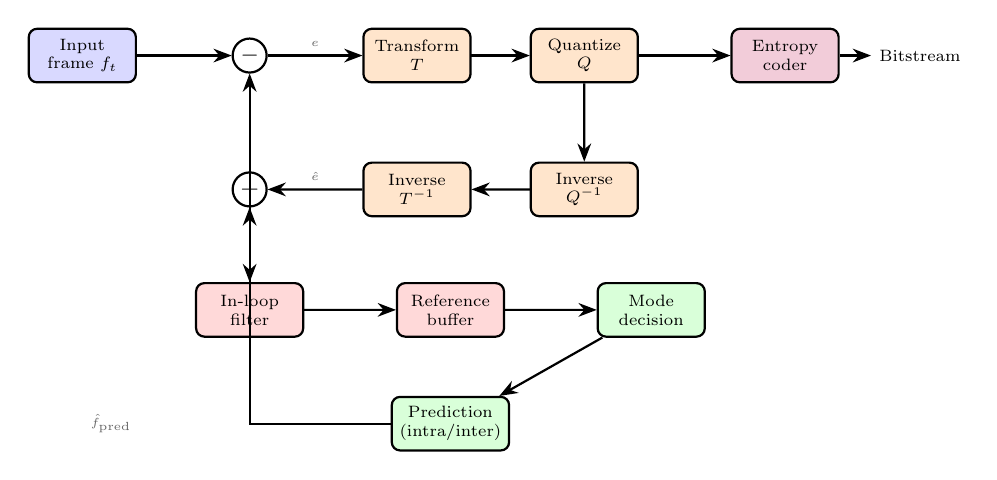
\begin{tikzpicture}[>=Stealth, scale=0.85, every node/.style={scale=0.85},
  block/.style={draw, rounded corners=3pt, minimum width=1.6cm,
    minimum height=0.8cm, font=\scriptsize, align=center, thick},
  arrow/.style={->, thick},
  label/.style={font=\tiny, text=black!60}]

% --- Input ---
\node[block, fill=blue!15] (input) at (0, 0) {Input\\frame $f_t$};

% --- Subtract ---
\node[draw, circle, inner sep=1.5pt, thick] (sub) at (2.5, 0) {$-$};

% --- Transform ---
\node[block, fill=orange!20] (transform) at (5, 0) {Transform\\$T$};

% --- Quantize ---
\node[block, fill=orange!20] (quant) at (7.5, 0) {Quantize\\$Q$};

% --- Entropy ---
\node[block, fill=purple!20] (entropy) at (10.5, 0) {Entropy\\coder};

% --- Bitstream ---
\node[font=\scriptsize, right=0.4cm of entropy] (bitstream) {Bitstream};

% --- Inverse Quantize ---
\node[block, fill=orange!20] (iquant) at (7.5, -2) {Inverse\\$Q^{-1}$};

% --- Inverse Transform ---
\node[block, fill=orange!20] (itransform) at (5, -2) {Inverse\\$T^{-1}$};

% --- Add ---
\node[draw, circle, inner sep=1.5pt, thick] (add) at (2.5, -2) {$+$};

% --- In-loop filter ---
\node[block, fill=red!15] (filter) at (2.5, -3.8) {In-loop\\filter};

% --- Reference buffer ---
\node[block, fill=red!15] (refbuf) at (5.5, -3.8) {Reference\\buffer};

% --- Mode decision ---
\node[block, fill=green!15] (mode) at (8.5, -3.8) {Mode\\decision};

% --- Prediction ---
\node[block, fill=green!15] (pred) at (5.5, -5.5) {Prediction\\(intra/inter)};

% --- Forward path ---
\draw[arrow] (input) -- (sub);
\draw[arrow] (sub) -- node[above, label] {$e$} (transform);
\draw[arrow] (transform) -- (quant);
\draw[arrow] (quant) -- (entropy);
\draw[arrow] (entropy) -- (bitstream);

% --- Reconstruction path ---
\draw[arrow] (quant) -- (iquant);
\draw[arrow] (iquant) -- (itransform);
\draw[arrow] (itransform) -- node[above, label] {$\hat{e}$} (add);

% --- Filter and buffer ---
\draw[arrow] (add) -- (filter);
\draw[arrow] (filter) -- (refbuf);

% --- Prediction feedback ---
\draw[arrow] (refbuf) -- (mode);
\draw[arrow] (mode) -- (pred);
\draw[arrow] (pred) -| (sub);
\draw[arrow] (pred) -| (add);

% --- Labels ---
\node[label, anchor=west] at (0, -5.5) {$\hat{f}_{\text{pred}}$};

\end{tikzpicture}
\caption{Block-based hybrid encoder architecture. Every codec from H.264
  through VVC follows this structure: predict each block from previously
  coded data (green), transform and quantize the residual (orange), entropy
  code the result (purple), then reconstruct and filter for future
  reference (red). The coding efficiency gap $\Delta$
  (eq.~\ref{eq:coding-gap}) arises from sub-optimal prediction, imperfect
  energy compaction, quantization beyond the rate-distortion bound, and
  entropy coding overhead.}
\label{fig:hybrid-encoder}
\end{figure}

The four sub-optimal components of Figure~\ref{fig:hybrid-encoder}---prediction,
transform, quantization, and entropy coding---each contribute to $\Delta$:
\begin{equation}
  \Delta \approx \Delta_{\text{pred}} + \Delta_{\text{transform}}
    + \Delta_{\text{quant}} + \Delta_{\text{entropy}}
  \label{eq:delta-decomp}
\end{equation}
Generational codec improvements reduce one or more of these terms. The codec
lineages in Sections~\ref{sec:mpeg-lineage}--\ref{sec:aom-lineage} trace
exactly which tools target which terms.

%% ---------------------------------------------------------------------------
\subsection{Transforms}
\label{sec:transforms}

The transform stage decorrelates the prediction residual, concentrating
energy into a few coefficients that can be efficiently quantized and coded.

\subsubsection{The KLT and Its DCT Approximation}
\label{sec:klt-dct}

The optimal decorrelating transform for a stationary source is the
\emph{Karhunen-Lo\`eve Transform} (KLT), whose basis vectors are the
eigenvectors of the input autocorrelation matrix $\mathbf{R}_{xx}$. For a
first-order Markov source with correlation $\rho$ (eq.~\ref{eq:spatial-autocorr}),
the KLT basis converges to the Type-II DCT as block size grows:
\begin{equation}
  C_k(n) = \alpha_k \cos\!\left[\frac{\pi k (2n+1)}{2N}\right],
  \quad k,n = 0, \ldots, N-1
  \label{eq:dct-ii}
\end{equation}
where $\alpha_0 = \sqrt{1/N}$ and $\alpha_k = \sqrt{2/N}$ for $k > 0$.

The energy compaction efficiency---the fraction of total energy captured by
the first $K$ of $N$ coefficients---is:
\begin{equation}
  \eta(K, N) = \frac{\sum_{k=0}^{K-1} \sigma_k^2}
    {\sum_{k=0}^{N-1} \sigma_k^2}
  \label{eq:energy-compaction}
\end{equation}
where $\sigma_k^2$ is the variance of the $k$-th transform coefficient.
For a typical intra residual with $\rho = 0.95$ and $N = 8$, the first 3
DCT coefficients capture approximately 95\% of the energy. This
concentration enables aggressive quantization of high-frequency coefficients
with minimal perceptual impact.

\subsubsection{Integer Transforms in Practice}
\label{sec:integer-transforms}

Practical codecs use integer approximations of the DCT to ensure bit-exact
encoder-decoder agreement. H.264 introduced a $4 \times 4$ integer
transform:
\begin{equation}
  \mathbf{H}_4 = \begin{pmatrix}
    1 &  1 &  1 &  1 \\
    2 &  1 & -1 & -2 \\
    1 & -1 & -1 &  1 \\
    1 & -2 &  2 & -1
  \end{pmatrix}
  \label{eq:h264-transform}
\end{equation}
The non-unity scaling factors are absorbed into the quantization step,
preserving exact integer arithmetic throughout the encode-decode loop.

Each codec generation expands the transform toolkit:

\begin{table}[ht]
\centering
\small
\renewcommand{\arraystretch}{1.4}
\begin{tabularx}{\textwidth}{lXXX}
\toprule
\textbf{Codec} & \textbf{Transform sizes} & \textbf{Transform types}
  & \textbf{Selection method} \\
\midrule
H.264 &
  $4\!\times\!4$, $8\!\times\!8$ &
  Integer DCT &
  Fixed per block size \\
VP9 &
  $4\!\times\!4$ to $32\!\times\!32$ &
  DCT, ADST &
  Row/column adaptive \\
HEVC &
  $4\!\times\!4$ to $32\!\times\!32$ &
  Integer DCT, DST ($4\!\times\!4$ intra) &
  Mode-dependent \\
AV1 &
  $4\!\times\!4$ to $64\!\times\!64$ &
  DCT, ADST, FlipADST, Identity &
  RD-optimized per block \\
VVC &
  $4\!\times\!4$ to $64\!\times\!64$ &
  DCT-II, DST-VII $+$ LFNST &
  RD-optimized $+$ secondary \\
\bottomrule
\end{tabularx}
\caption{Transform sizes and types across codec generations. AV1 applies
  four 1D transform types independently to rows and columns, yielding
  16~possible 2D combinations per block. VVC adds a non-separable secondary
  transform (LFNST) applied to low-frequency coefficients after the primary
  separable transform.}
\label{tab:transforms}
\end{table}

The Asymmetric Discrete Sine Transform (ADST) used in VP9 and AV1 is
particularly effective for intra-predicted residuals, which tend to have
larger magnitudes near the prediction boundary. AV1's FlipADST extends
this to blocks where the large residuals are on the opposite edge, while
the Identity transform (skip) handles blocks where the residual is already
well-distributed in the spatial domain.

The progression from fixed transforms (H.264) to RD-optimized multi-type
selection (AV1, VVC) directly reduces $\Delta_{\text{transform}}$ in
(\ref{eq:delta-decomp}): better energy compaction means fewer bits are
needed to represent the same residual at a given distortion level.

%% ---------------------------------------------------------------------------
\subsection{Motion Estimation and Inter Prediction}
\label{sec:motion}

Inter prediction exploits temporal redundancy by predicting blocks in the
current frame from previously coded reference frames. This is the single
largest source of compression gain---the prediction residual
(eq.~\ref{eq:residual}) typically has 10--20$\times$ less energy than the
original signal.

\subsubsection{Block Matching and Motion Vectors}
\label{sec:block-matching}

The encoder searches for the best-matching region in a reference frame by
minimizing a cost function over candidate displacement vectors
$\mathbf{d} = (d_x, d_y)$:
\begin{equation}
  \text{SAD}(\mathbf{d}) = \sum_{(x,y) \in B}
    \left| f_t(x,y) - f_{t-1}(x + d_x,\, y + d_y) \right|
  \label{eq:sad}
\end{equation}
The Sum of Absolute Differences (SAD) is the simplest distortion measure.
A better rate-distortion proxy is the Sum of Absolute Transformed
Differences (SATD), which applies the Hadamard transform before summation:
\begin{equation}
  \text{SATD}(\mathbf{d}) = \sum \left| \mathbf{H}
    \cdot \left( f_t - f_{t-1}(\mathbf{d}) \right) \right|
  \label{eq:satd}
\end{equation}
SATD approximates the post-transform energy and thus better predicts the
actual coded bit cost. Rate-constrained motion estimation augments the
distortion with a motion vector coding cost:
\begin{equation}
  \mathbf{d}^* = \arg\min_{\mathbf{d}} \left[
    \text{SATD}(\mathbf{d}) + \lambda_{\text{motion}} \cdot R(\mathbf{d})
  \right]
  \label{eq:rcme}
\end{equation}
where $R(\mathbf{d})$ is the bit cost of encoding the motion vector
relative to a predictor.

\subsubsection{Sub-Pixel Interpolation}
\label{sec:subpixel}

Motion in natural video rarely aligns to integer pixel positions. All modern
codecs perform sub-pixel motion compensation by interpolating reference
frame samples at fractional positions.

H.264 uses a 6-tap filter for half-pixel luma interpolation:
\begin{equation}
  h_{\frac{1}{2}} = \{1, -5, 20, 20, -5, 1\} / 32
  \label{eq:h264-halfpel}
\end{equation}
with quarter-pixel positions obtained by bilinear averaging of integer and
half-pixel samples. HEVC extends this to an 8-tap filter for half-pixel and
a 7-tap filter for quarter-pixel positions. AV1 introduces a switchable
filter bank with three 8-tap options---Regular (sharp), Smooth (low-pass),
and Sharp (high-frequency preserving)---selected per block via RD
optimization. VVC adds DMVR (Decoder-side Motion Vector Refinement) and
BDOF (Bi-Directional Optical Flow) for sub-pixel refinement at the decoder
without additional signaling bits.

The progression from H.264's fixed 6-tap filter to AV1's switchable bank
reduces $\Delta_{\text{pred}}$: better interpolation means smaller
prediction residuals, which require fewer bits.

\subsubsection{Advanced Inter Prediction Tools}
\label{sec:advanced-inter}

Beyond basic block matching, each codec generation adds tools to handle
complex motion and occlusion:

\begin{itemize}
\item \textbf{Multiple reference frames.} H.264 introduced up to 16
  reference frames; practical WebRTC encoders use 1--3 for latency reasons.
  More references improve prediction for periodic motion and uncovered
  backgrounds.

\item \textbf{Bi-prediction.} A weighted average of predictions from two
  reference frames, reducing noise and handling gradual scene changes.
  Available from H.264 onward (in B-frames) and in AV1's compound modes.

\item \textbf{Compound prediction (AV1).} Wedge masks and
  difference-weighted blending combine two predictions at the block level,
  handling occlusion boundaries where a single motion model fails.

\item \textbf{Overlapped Block Motion Compensation (AV1).} Blends
  predictions from neighboring blocks at motion boundaries, reducing
  blocking artifacts without post-processing.

\item \textbf{Warped motion (AV1).} An affine model with up to 6
  parameters handles rotation, zoom, and perspective---common in
  screen sharing and camera motion.

\item \textbf{VVC additions.} Geometric Partitioning Mode (non-rectangular
  block splits for motion boundaries), BDOF (optical flow refinement at the
  decoder), and DMVR (decoder-side MV refinement using bilateral matching).
\end{itemize}

\excursus{Excursus: Motion estimation in real-time encoding.}{Full-search
block matching has complexity $O(N^2 \cdot S^2)$ where $N$ is the block
dimension and $S$ is the search range in pixels. For a $64\!\times\!64$
block with $S = 64$, this is ${\sim}17$ million SAD operations per
block---far too expensive for real-time encoding. WebRTC encoders use
hierarchical search patterns (diamond, hexagon) that reduce complexity to
$O(N^2 \cdot \log S)$ with typically $< 5\%$ rate-distortion penalty
relative to full search. This is why real-time encoders use only a subset
of each codec's inter prediction tools: the full tool set is available
for offline encoding, but the real-time constraint forces aggressive
pruning of the mode decision search space.}

%% ---------------------------------------------------------------------------
\subsection{Quantization}
\label{sec:quantization}

Quantization is the sole lossy step in the hybrid coding pipeline. It maps
continuous-valued (or high-precision integer) transform coefficients to a
discrete set of reconstruction levels, introducing controlled information
loss to achieve the target bit rate.

\subsubsection{Scalar Quantization}

Uniform scalar quantization maps coefficient $c$ to a quantization index:
\begin{equation}
  q = \text{round}\!\left(\frac{c}{Q_{\text{step}}}\right), \quad
  \hat{c} = q \cdot Q_{\text{step}}
  \label{eq:uniform-quant}
\end{equation}
Modern codecs use \emph{dead-zone quantization}, where coefficients near
zero are mapped to zero more aggressively than uniform rounding predicts:
\begin{equation}
  q = \text{sign}(c) \cdot \left\lfloor
    \frac{|c| - f \cdot Q_{\text{step}}}{Q_{\text{step}}}
  \right\rfloor
  \label{eq:deadzone}
\end{equation}
where $f \in [0, 0.5)$ controls the dead-zone width. Dead-zone
quantization increases sparsity---the fraction of zero-valued
coefficients---which dramatically improves entropy coding efficiency.

\subsubsection{QP-to-Step-Size Mapping}

The quantization parameter (QP) controls the step size via an exponential
relationship. In the H.264/HEVC/VVC family:
\begin{equation}
  Q_{\text{step}} = Q_0 \cdot 2^{(QP - QP_0)/6}
  \label{eq:qp-mapping}
\end{equation}
A 6-unit increase in QP doubles the step size, approximately doubling the
bit rate. AV1 uses a similar but codec-specific mapping with separate QP
values for DC and AC coefficients, plus per-segment QP adjustment for
region-of-interest coding.

\subsubsection{Quantization Distortion}

For a single coefficient under uniform quantization at high rate, the
distortion is:
\begin{equation}
  D_q = \frac{Q_{\text{step}}^2}{12}
  \label{eq:quant-distortion}
\end{equation}
For a block of $N$ transform coefficients where $K$ survive quantization
(nonzero) and $N - K$ are quantized to zero:
\begin{equation}
  D_{\text{block}} \approx K \cdot \frac{Q_{\text{step}}^2}{12}
    + \sum_{k \notin K} c_k^2
  \label{eq:block-distortion}
\end{equation}
The second term represents the energy of coefficients eliminated by the
dead zone---information permanently discarded. The QP is thus the primary
control knob for navigating the rate-distortion curve in
Figure~\ref{fig:rate-distortion}. The WebCodecs \texttt{VideoEncoder} API
exposes this control via the \texttt{quantizer} configuration parameter,
giving JavaScript applications direct access to this fundamental
trade-off.

%% ---------------------------------------------------------------------------
\subsection{Entropy Coding}
\label{sec:entropy-coding}

After quantization, the surviving coefficients and all side information
(motion vectors, prediction modes, block partitions) must be losslessly
compressed. The entropy coder converts these symbols into a bitstream,
approaching the conditional entropy $H(X|\text{context})$ as closely as
possible. The gap between the entropy coder's output rate and the true
conditional entropy is $\Delta_{\text{entropy}}$ in
(\ref{eq:delta-decomp}).

\subsubsection{Context-Adaptive Binary Arithmetic Coding (CABAC)}
\label{sec:cabac}

CABAC, used in H.264, HEVC, and VVC, encodes each syntax element as a
sequence of binary decisions (bins). For each bin, the arithmetic coder
subdivides the current interval $[L, H)$ based on the estimated
probability $p$:
\begin{equation}
  [L, H) \to \begin{cases}
    [L,\; L + p \cdot (H - L)) & \text{if bin} = 0 \\
    [L + p \cdot (H - L),\; H) & \text{if bin} = 1
  \end{cases}
  \label{eq:arithmetic-coding}
\end{equation}
The theoretical output length approaches the entropy:
\begin{equation}
  \ell \to \sum_{i=1}^{n} -\log_2 p(b_i \mid \text{ctx}_i)
  \label{eq:cabac-length}
\end{equation}
CABAC achieves redundancy below 0.01 bits/symbol relative to the true
conditional entropy---near-optimal compression.

Context modeling is the key to CABAC's effectiveness. Each bin type has an
associated context, whose probability is updated after each observation via
a state-machine-based exponential moving average:
\begin{equation}
  p_{k+1} = p_k + \alpha(s_k) \cdot (b_k - p_k)
  \label{eq:cabac-update}
\end{equation}
where $\alpha(s_k)$ is a state-dependent adaptation rate, indexed by a
lookup table with 64 states (H.264) or 128 states (HEVC/VVC). This design
avoids floating-point arithmetic entirely.

CABAC also provides a \emph{bypass mode} for bins with approximately
uniform probability (e.g., sign bits, high-magnitude coefficient levels),
which skips the context lookup and probability estimation for throughput.

\subsubsection{Multi-Symbol Arithmetic Coding in AV1}
\label{sec:av1-entropy}

AV1 departs from binary arithmetic coding. Its entropy coder operates on
multi-symbol alphabets using CDF (Cumulative Distribution Function) tables:
\begin{equation}
  \text{Encode symbol } s: \quad
  [L, H) \to \left[L + \frac{\text{CDF}(s-1)}{M} \cdot (H-L),\;
    L + \frac{\text{CDF}(s)}{M} \cdot (H-L)\right)
  \label{eq:av1-entropy}
\end{equation}
where $M$ is the total frequency count. CDF tables are adapted after
each symbol:
\begin{equation}
  \text{CDF}_{k+1}(s) = \text{CDF}_k(s) + \left\lfloor
    \frac{\text{target}(s) - \text{CDF}_k(s)}{n}
  \right\rfloor
  \label{eq:cdf-update}
\end{equation}
where $n$ controls the adaptation rate. Multi-symbol coding is more
efficient than CABAC's binarization for syntax elements with moderate
alphabet sizes (e.g., intra prediction modes, transform types), as it
avoids the overhead of converting each symbol into a binary tree of
decisions.

\begin{table}[ht]
\centering
\small
\renewcommand{\arraystretch}{1.4}
\begin{tabularx}{\textwidth}{lXXXXX}
\toprule
\textbf{Feature} & \textbf{H.264} & \textbf{HEVC} & \textbf{VP9}
  & \textbf{AV1} & \textbf{VVC} \\
\midrule
Method &
  Binary AC &
  Binary AC &
  Boolean AC &
  Multi-sym AC &
  Binary AC \\
Contexts &
  ${\sim}400$ &
  ${\sim}200$ &
  ${\sim}900$ &
  ${\sim}300$ &
  ${\sim}700$ \\
Adaptation &
  64-state LUT &
  128-state LUT &
  Counter &
  CDF update &
  128-state LUT \\
Bypass mode &
  Yes &
  Yes &
  N/A &
  N/A &
  Yes \\
Parallelism &
  Slice &
  WPP / Tiles &
  Tiles &
  Tiles &
  WPP / Tiles \\
\bottomrule
\end{tabularx}
\caption{Entropy coding comparison across codecs. HEVC reduced context
  count relative to H.264 for throughput; VVC increased it again for
  improved compression. AV1's multi-symbol approach operates on full
  alphabets rather than binary decompositions.}
\label{tab:entropy-coding}
\end{table}

The frame entropy $\hat{H}(f_t)$ from eq.~(\ref{eq:frame-entropy}) is
ultimately determined by how well the entropy coder's probability model
matches the true symbol distribution. Both CABAC and AV1's multi-symbol
coder achieve near-zero entropy coding gaps; the remaining
$\Delta_{\text{entropy}}$ arises primarily from context model mismatch on
non-stationary content (scene changes, sudden motion onset).

%% ---------------------------------------------------------------------------
\subsection{In-Loop Filtering}
\label{sec:filtering}

Block-based coding introduces visible artifacts at block boundaries:
discontinuities from independent quantization of adjacent blocks, and
ringing from coefficient truncation. In-loop filters reduce these artifacts
\emph{before} the reconstructed frame enters the reference buffer, improving
prediction quality for subsequent frames and thus reducing
$\Delta_{\text{pred}}$.

\begin{itemize}
\item \textbf{Deblocking filter (all codecs).} Smooths discontinuities
  at block edges, with filter strength adapted to the quantization level
  and local gradient. Introduced in H.264; refined in each subsequent
  codec.

\item \textbf{Sample Adaptive Offset---SAO (HEVC).} Classifies
  reconstructed samples by intensity or edge direction and applies
  per-class offsets to reduce systematic bias introduced by quantization.

\item \textbf{Constrained Directional Enhancement Filter---CDEF (AV1).}
  A directional filter that identifies edge orientation per
  $8\!\times\!8$ block and applies filtering only along the edge,
  preserving sharpness while reducing ringing.

\item \textbf{Loop Restoration Filter (AV1).} A switchable per-tile
  filter choosing between a Wiener filter (FIR designed to minimize MSE
  between original and reconstruction) and a Self-Guided filter (non-linear
  denoising based on guided image filtering). This is AV1's most powerful
  quality enhancement tool.

\item \textbf{Adaptive Loop Filter---ALF (VVC).} A diamond-shaped filter
  with coefficients signaled per frame, applied adaptively per
  $4\!\times\!4$ block based on local classification. Subsumes HEVC's
  SAO functionality.
\end{itemize}

The evolution from simple deblocking (H.264) to multi-stage adaptive
filtering (AV1: deblocking $\to$ CDEF $\to$ loop restoration) exemplifies
how each codec generation reduces $\Delta_{\text{pred}}$ by improving
reference frame quality.

%% ---------------------------------------------------------------------------
\subsection{Codec Lineage: MPEG/ITU Family}
\label{sec:mpeg-lineage}

The MPEG/ITU standardization track has produced three codec generations
relevant to the 2021--2031 timeframe of this document.

\subsubsection{H.264/AVC (2003)}
\label{sec:h264}

H.264 defined the modern era of video compression and remains the most
widely deployed codec. Its key innovations over its predecessors (H.263,
MPEG-2):

\begin{itemize}
\item Variable block sizes: $16\!\times\!16$ macroblock partitioned into
  $16\!\times\!8$, $8\!\times\!16$, $8\!\times\!8$, $8\!\times\!4$,
  $4\!\times\!8$, and $4\!\times\!4$ sub-partitions for motion
  compensation.

\item Quarter-pixel motion compensation with 6-tap interpolation
  (eq.~\ref{eq:h264-halfpel}).

\item Context-adaptive intra prediction: 9~angular modes for
  $4\!\times\!4$ blocks, 4~modes for $16\!\times\!16$.

\item Dual entropy coding: CAVLC (simpler, faster) and CABAC
  (Section~\ref{sec:cabac}; 10--15\% better compression).

\item In-loop deblocking filter, mandatory for the decoder.

\item Multiple reference frames (up to 16) and weighted prediction.
\end{itemize}

Three profiles are relevant to WebRTC: \textbf{Constrained Baseline}
(no CABAC, no B-frames, lowest complexity---the mandatory WebRTC profile),
\textbf{Main} (CABAC, B-frames, ${\sim}$10\% better compression), and
\textbf{High} ($8\!\times\!8$ transform, adaptive quantization matrices,
${\sim}$15\% better).

At the 720p/30fps reference point, H.264 Constrained Baseline operates at
approximately 2.0--2.5~Mbps for ``good'' quality (PSNR ${\sim}$37~dB),
corresponding to $\Delta_{\text{H.264}} \approx 2.1$ from
Appendix~\ref{app:info-theory}. H.264 was the only codec Safari supported
in 2021 (Section~3.1), and its higher $\Delta$ is directly responsible
for the bandwidth disparity between Safari-only and VP9-capable sessions
documented in the main text.

\subsubsection{H.265/HEVC (2013)}
\label{sec:hevc}

HEVC replaced H.264's fixed $16\!\times\!16$ macroblock with a recursive
Coding Tree Unit (CTU) of up to $64\!\times\!64$ pixels, using quad-tree
partitioning down to $8\!\times\!8$. Key advances:

\begin{itemize}
\item 35 intra prediction angular directions (vs.\ H.264's 9).
\item Transform sizes from $4\!\times\!4$ to $32\!\times\!32$, with
  DST for $4\!\times\!4$ intra blocks.
\item Advanced Motion Vector Prediction (AMVP): two MVP candidates selected
  from spatial and temporal neighbors, replacing H.264's less structured
  motion vector prediction.
\item Merge mode: inherits the full motion information (MV, reference
  index, prediction direction) from a neighboring block, requiring zero
  additional motion bits.
\item Sample Adaptive Offset (SAO) in-loop filter.
\item Parallel processing: Wavefront Parallel Processing (WPP) and tiles.
\end{itemize}

HEVC achieves approximately 40\% rate reduction over H.264 at equivalent
PSNR. However, HEVC is absent from WebRTC entirely---not due to technical
limitations, but due to patent licensing.

\excursus{Excursus: Why no HEVC in WebRTC?}{HEVC's patent licensing is
fragmented across three separate pools (MPEG-LA, HEVC Advance, Velos Media)
plus independent licensors who are not members of any pool. The resulting
uncertainty about total royalty cost---estimated at \$0.20--\$0.40 per device
for some use cases---led Google, Mozilla, Cisco, and others to form the
Alliance for Open Media (AOM) in 2015 and develop AV1 as a royalty-free
alternative. This patent-driven fork is why the WebRTC ecosystem followed the
VP8$\to$VP9$\to$AV1 path rather than H.264$\to$HEVC$\to$VVC, and why the two
codec families must be understood in parallel.}

\subsubsection{H.266/VVC (2020)}
\label{sec:vvc}

VVC extends HEVC's quad-tree with binary and ternary splits, creating a
\emph{multi-type tree} (MTT) that enables asymmetric block shapes (e.g.,
$32\!\times\!8$, $8\!\times\!32$, $32\!\times\!4$). Additional
innovations:

\begin{itemize}
\item 67 intra prediction directions plus Matrix-based Intra Prediction
  (MIP), which applies a learned linear transform to neighboring samples.

\item Multiple Transform Selection (MTS): explicit signaling of DCT-II or
  DST-VII per block, plus the Low-Frequency Non-Separable Transform
  (LFNST)---a $16\!\times\!16$ or $8\!\times\!8$ non-separable transform
  applied to low-frequency coefficients after the primary separable
  transform.

\item Affine motion model: 4-parameter (translation $+$ rotation/scaling)
  or 6-parameter (full affine) motion, derived from control point MVs at
  block corners.

\item Decoder-side tools: DMVR refines motion vectors at the decoder using
  bilateral template matching; BDOF applies optical flow equations to
  refine bi-predicted samples, both without additional signaling bits.

\item Geometric Partitioning Mode: divides a block diagonally for separate
  motion compensation of each partition, targeting motion boundaries.

\item Adaptive Loop Filter (ALF): a diamond-shaped Wiener filter with
  coefficients signaled per frame and applied adaptively per
  $4\!\times\!4$ block.
\end{itemize}

VVC achieves approximately 30--50\% rate reduction over HEVC, placing it at
$\Delta_{\text{VVC}} \approx 0.3$. Its relevance to this document is
forward-looking: VVC may appear in WebCodecs codec registries by
${\sim}$2030 if licensing concerns are resolved, and its tool set
represents the current efficiency frontier against which AV1's performance
should be measured.

%% ---------------------------------------------------------------------------
\subsection{Codec Lineage: Google/AOM Family}
\label{sec:aom-lineage}

The royalty-free codec family dominates the WebRTC ecosystem. Its
development was driven by the patent licensing concerns described in the
HEVC excursus above.

\subsubsection{VP8 (2010)}
\label{sec:vp8}

VP8 was Google's first open-source video codec, released alongside the
WebM container. Its design is conservative:

\begin{itemize}
\item $16\!\times\!16$ macroblocks with $4\!\times\!4$ subblock partitions.
\item $4\!\times\!4$ Walsh-Hadamard Transform (WHT) for DC coefficients,
  $4\!\times\!4$ DCT for AC coefficients.
\item Boolean arithmetic coder with tree-structured syntax (single-bit
  alphabet).
\item 4 intra prediction modes for $16\!\times\!16$, 10 for
  $4\!\times\!4$ subblocks.
\item Simple loop filter with per-edge strength adaptation.
\item Single reference frame for WebRTC (plus a ``golden'' frame for
  screen content).
\end{itemize}

VP8's compression efficiency is roughly equivalent to H.264 Constrained
Baseline. It served as the baseline WebRTC codec---supported by Chrome and
Firefox since WebRTC~1.0---but has been superseded by VP9 in all modern
deployments.

\subsubsection{VP9 (2013)}
\label{sec:vp9}

VP9 introduced a superblock architecture and several tools that brought it
within range of HEVC:

\begin{itemize}
\item $64\!\times\!64$ superblocks with recursive quad-tree partitioning
  down to $4\!\times\!4$.
\item 10 intra prediction modes.
\item Transforms: DCT and ADST applied independently per row and column,
  at sizes from $4\!\times\!4$ to $32\!\times\!32$.
\item Switchable interpolation filters: 8-tap Regular, Smooth, and
  Sharp, selected per block.
\item Compound prediction: weighted average from two reference frames.
\item Segmentation: per-segment QP adjustment for region-of-interest
  coding.
\end{itemize}

VP9 achieves approximately 35\% rate reduction over H.264
(eq.~\ref{eq:vp9-savings}), placing it at $\Delta_{\text{VP9}} \approx 0.8$.
VP9 is the dominant WebRTC codec in Chrome and Firefox as of March~2026,
and its temporal SVC support (Section~\ref{sec:svc}) is the primary
mechanism enabling adaptive quality in multi-participant calls.

\subsubsection{AV1 (2018)}
\label{sec:av1}

AV1 represents the most ambitious single-generation improvement in the
royalty-free family. Its tool set approaches VVC in breadth while
maintaining royalty-free status:

\begin{itemize}
\item $128\!\times\!128$ superblocks with flexible partitioning (quad-tree
  plus rectangular splits) down to $4\!\times\!4$.

\item 56+ directional intra prediction modes plus non-directional modes
  (Paeth, Smooth variants, DC).

\item Full inter prediction toolkit: OBMC, warped motion (affine),
  compound modes (Wedge, Difference-weighted), inter-intra compound
  prediction.

\item 16 transform type combinations ($4$ 1D types $\times$ rows/columns),
  at sizes up to $64\!\times\!64$.

\item Film Grain Synthesis: the encoder characterizes noise/grain
  parameters and transmits them as metadata; the decoder re-synthesizes
  grain after reconstruction. This removes non-compressible high-frequency
  noise from the coding loop---a major bitrate saving for camera-captured
  content.

\item Multi-stage in-loop filtering: deblocking $\to$ CDEF $\to$ loop
  restoration (Wiener or Self-Guided), as described in
  Section~\ref{sec:filtering}.

\item Multi-symbol arithmetic coding with CDF-based context adaptation
  (Section~\ref{sec:av1-entropy}).
\end{itemize}

AV1 achieves approximately 30\% rate reduction over VP9
(eq.~\ref{eq:av1-savings}), a cumulative ${\sim}$54\% over H.264, placing
it at $\Delta_{\text{AV1}} \approx 0.5$ with current hardware encoders and
approaching 0.4 by 2030 as encoder implementations mature.

AV1's tools directly explain why its $\Delta$ is smaller than VP9's:
more transform types capture residual structure better (reducing
$\Delta_{\text{transform}}$), warped and compound motion reduce prediction
residual energy (reducing $\Delta_{\text{pred}}$), and film grain synthesis
removes non-compressible variance from the coding loop (effectively
reducing the source variance $\sigma^2$ that the codec must represent).

%% ---------------------------------------------------------------------------
\subsection{Block Partitioning: A Generational Comparison}
\label{sec:partitioning}

Block partitioning is the most architecturally consequential difference
between codec generations. Larger and more flexible partitions allow the
encoder to match block boundaries to content structure---smooth regions
get large blocks (few bits for partition overhead), detailed regions get
small blocks (better prediction accuracy).

\begin{figure}[ht]
\centering
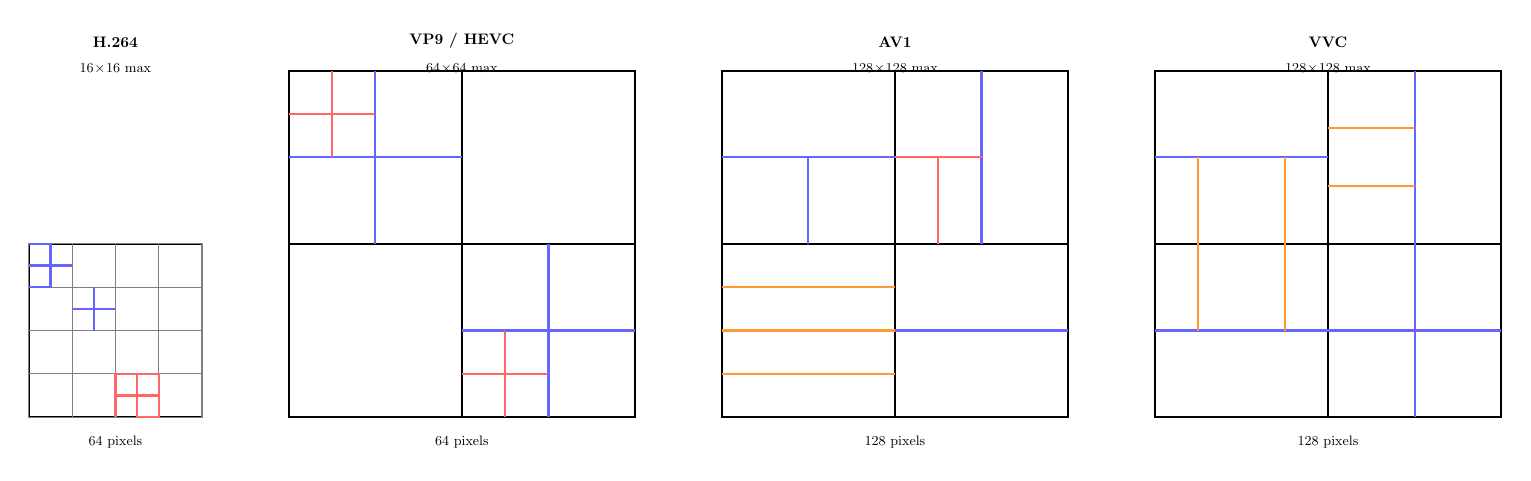
\begin{tikzpicture}[>=Stealth, scale=0.55, every node/.style={scale=0.55}]

% --- H.264 panel ---
\begin{scope}[xshift=0cm]
  \node[font=\normalsize\bfseries, anchor=south] at (2, 8.4) {H.264};
  \node[font=\small, anchor=south] at (2, 7.8) {$16\!\times\!16$ max};
  % 4x4 grid of 16x16 macroblocks in a 64x64 region
  \draw[thick] (0,0) rectangle (4,4);
  \draw[thick] (0,0) rectangle (4,4);
  % macroblock grid
  \foreach \x in {0,1,2,3} {
    \foreach \y in {0,1,2,3} {
      \draw[gray] (\x, \y) rectangle (\x+1, \y+1);
    }
  }
  % show some sub-partitions
  \draw[blue!60, thick] (0,3) -- (0.5,3) -- (0.5,4) -- (0,4);
  \draw[blue!60, thick] (0.5,3) -- (0.5,4);
  \draw[blue!60, thick] (0,3.5) -- (1,3.5);
  % 8x8 in another
  \draw[blue!60, thick] (1,2.5) -- (2,2.5);
  \draw[blue!60, thick] (1.5,2) -- (1.5,3);
  % 4x4 in another
  \draw[red!60, thick] (2,0) -- (2,1) -- (3,1) -- (3,0);
  \draw[red!60, thick] (2.5,0) -- (2.5,0.5);
  \draw[red!60, thick] (2,0.5) -- (2.5,0.5);
  \draw[red!60, thick] (2.5,0.5) -- (2.5,1);
  \draw[red!60, thick] (2.5,0) -- (3,0) -- (3,0.5) -- (2.5,0.5);
  % Scale label
  \node[font=\small, anchor=north] at (2, -0.3) {64 pixels};
\end{scope}

% --- VP9/HEVC panel ---
\begin{scope}[xshift=6cm]
  \node[font=\normalsize\bfseries, anchor=south] at (4, 8.4) {VP9 / HEVC};
  \node[font=\small, anchor=south] at (4, 7.8) {$64\!\times\!64$ max};
  % One 64x64 superblock
  \draw[thick] (0,0) rectangle (8,8);
  % quad-tree splits
  \draw[thick] (4,0) -- (4,8);
  \draw[thick] (0,4) -- (8,4);
  % further splits in top-left quadrant
  \draw[blue!60, thick] (2,4) -- (2,8);
  \draw[blue!60, thick] (0,6) -- (4,6);
  % further split in top-left-top-left
  \draw[red!60, thick] (1,6) -- (1,8);
  \draw[red!60, thick] (0,7) -- (2,7);
  % split bottom-right quadrant
  \draw[blue!60, thick] (6,0) -- (6,4);
  \draw[blue!60, thick] (4,2) -- (8,2);
  % deeper in bottom-right-bottom-left
  \draw[red!60, thick] (5,0) -- (5,2);
  \draw[red!60, thick] (4,1) -- (6,1);
  % Scale label
  \node[font=\small, anchor=north] at (4, -0.3) {64 pixels};
\end{scope}

% --- AV1 panel ---
\begin{scope}[xshift=16cm]
  \node[font=\normalsize\bfseries, anchor=south] at (4, 8.4) {AV1};
  \node[font=\small, anchor=south] at (4, 7.8) {$128\!\times\!128$ max};
  % 128x128 shown as 8x8 grid (each cell = 16px)
  \draw[thick] (0,0) rectangle (8,8);
  % quad split: top half / bottom half
  \draw[thick] (4,0) -- (4,8);
  \draw[thick] (0,4) -- (8,4);
  % rectangular splits in top-left
  \draw[blue!60, thick] (0,6) -- (4,6);
  \draw[blue!60, thick] (2,4) -- (2,6);
  % asymmetric in bottom-left (4:1 rect)
  \draw[orange!80, thick] (0,3) -- (4,3);
  \draw[orange!80, thick] (0,2) -- (4,2);
  \draw[orange!80, thick] (0,1) -- (4,1);
  % quad + rect in top-right
  \draw[blue!60, thick] (6,4) -- (6,8);
  \draw[red!60, thick] (4,6) -- (6,6);
  \draw[red!60, thick] (5,4) -- (5,6);
  % bottom-right: large blocks
  \draw[blue!60, thick] (4,2) -- (8,2);
  % Scale label
  \node[font=\small, anchor=north] at (4, -0.3) {128 pixels};
\end{scope}

% --- VVC panel ---
\begin{scope}[xshift=26cm]
  \node[font=\normalsize\bfseries, anchor=south] at (4, 8.4) {VVC};
  \node[font=\small, anchor=south] at (4, 7.8) {$128\!\times\!128$ max};
  \draw[thick] (0,0) rectangle (8,8);
  % quad split
  \draw[thick] (4,0) -- (4,8);
  \draw[thick] (0,4) -- (8,4);
  % binary split (horizontal) in top-left
  \draw[blue!60, thick] (0,6) -- (4,6);
  % ternary split (vertical) in top-left-bottom
  \draw[orange!80, thick] (1,4) -- (1,6);
  \draw[orange!80, thick] (3,4) -- (3,6);
  % binary split (vertical) in top-right
  \draw[blue!60, thick] (6,4) -- (6,8);
  % ternary horizontal in top-right-left
  \draw[orange!80, thick] (4,5.33) -- (6,5.33);
  \draw[orange!80, thick] (4,6.67) -- (6,6.67);
  % bottom-left: binary horizontal
  \draw[blue!60, thick] (0,2) -- (4,2);
  % deeper ternary in bottom-left-top
  \draw[orange!80, thick] (1,2) -- (1,4);
  \draw[orange!80, thick] (3,2) -- (3,4);
  % bottom-right: mostly large
  \draw[blue!60, thick] (6,0) -- (6,4);
  \draw[blue!60, thick] (4,2) -- (8,2);
  % Scale label
  \node[font=\small, anchor=north] at (4, -0.3) {128 pixels};
\end{scope}

\end{tikzpicture}
\caption{Block partitioning comparison across codec generations. H.264 is
  limited to $16\!\times\!16$ macroblocks with fixed sub-partitions (left).
  VP9/HEVC use quad-tree partitioning within $64\!\times\!64$ superblocks
  (center-left). AV1 extends to $128\!\times\!128$ with quad-tree plus
  rectangular splits (center-right). VVC adds binary and ternary splits for
  maximum flexibility (right). Blue lines show first-level splits; red
  shows deeper partitioning; orange shows asymmetric/ternary splits.}
\label{fig:block-partitioning}
\end{figure}

\begin{table}[ht]
\centering
\small
\renewcommand{\arraystretch}{1.4}
\begin{tabularx}{\textwidth}{lXXXXX}
\toprule
\textbf{Feature} & \textbf{H.264} & \textbf{VP9} & \textbf{HEVC}
  & \textbf{AV1} & \textbf{VVC} \\
\midrule
Max block &
  $16\!\times\!16$ &
  $64\!\times\!64$ &
  $64\!\times\!64$ &
  $128\!\times\!128$ &
  $128\!\times\!128$ \\
Min block &
  $4\!\times\!4$ &
  $4\!\times\!4$ &
  $8\!\times\!8$ &
  $4\!\times\!4$ &
  $4\!\times\!4$ \\
Split types &
  Fixed partitions &
  Quad-tree &
  Quad-tree &
  Quad $+$ rect &
  Quad $+$ BT $+$ TT \\
Asymmetric &
  Limited &
  No &
  No &
  4:1 rectangles &
  Full (BT/TT) \\
\bottomrule
\end{tabularx}
\caption{Block partitioning capabilities by codec. BT = binary tree
  (horizontal or vertical), TT = ternary tree (1:2:1 split). Larger maximum
  blocks reduce overhead for homogeneous regions; asymmetric splits improve
  partitioning efficiency at content boundaries.}
\label{tab:partitioning}
\end{table}

%% ---------------------------------------------------------------------------
\subsection{Rate-Distortion Operating Points by Codec}
\label{sec:rd-comparison}

The codec-specific analyses of
Sections~\ref{sec:mpeg-lineage}--\ref{sec:aom-lineage} can be unified
through the Bj\o ntegaard Delta Rate (BD-Rate), the standard metric for
comparing codec efficiency. BD-Rate computes the average percentage rate
difference between two codecs at equivalent distortion by integrating the
difference between their rate-distortion curves fit as cubic polynomials in
PSNR-vs-log-rate space:
\begin{equation}
  \text{BD-Rate} = \frac{1}{\Delta\text{PSNR}}
    \int_{\text{PSNR}_{\min}}^{\text{PSNR}_{\max}}
    \left[ \ln R_A(p) - \ln R_B(p) \right] dp
  \label{eq:bd-rate}
\end{equation}
A negative BD-Rate indicates that codec~$A$ requires fewer bits than
codec~$B$ at the same quality.

\begin{figure}[ht]
\centering
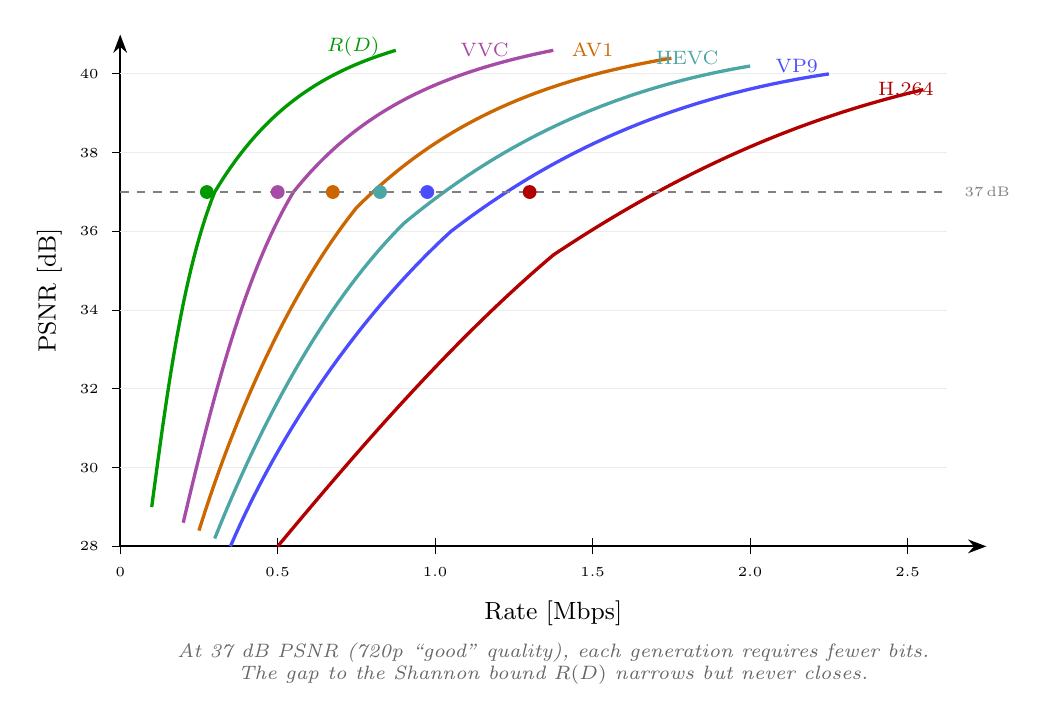
\begin{tikzpicture}[>=Stealth]

% --- Axes ---
\draw[->, thick] (0, 0) -- (11, 0);
\draw[->, thick] (0, 0) -- (0, 6.5);

% --- Axis titles ---
\node[font=\small] at (5.5, -0.85) {Rate [Mbps]};
\node[font=\small, rotate=90] at (-0.9, 3.25) {PSNR [dB]};

% --- X-axis labels ---
\foreach \x/\lab in {0/0, 2/0.5, 4/1.0, 6/1.5, 8/2.0, 10/2.5} {
  \draw (\x, -0.1) -- (\x, 0.1);
  \node[font=\tiny, anchor=north] at (\x, -0.15) {\lab};
}

% --- Y-axis labels ---
\foreach \y/\lab in {0/28, 1/30, 2/32, 3/34, 4/36, 5/38, 6/40} {
  \draw (-0.1, \y) -- (0.1, \y);
  \node[font=\tiny, anchor=east] at (-0.15, \y) {\lab};
}

% --- Grid ---
\foreach \y in {1,2,3,4,5,6} {
  \draw[gray!15] (0, \y) -- (10.5, \y);
}

% --- Shannon R(D) bound (leftmost curve) ---
\draw[very thick, green!60!black]
  (0.4, 0.5) .. controls (0.6, 2) and (0.8, 3.5) ..
  (1.2, 4.5) .. controls (1.8, 5.5) and (2.5, 6.0) ..
  (3.5, 6.3);
\node[font=\scriptsize, green!60!black, anchor=south west] at (2.5, 6.1)
  {$R(D)$};

% --- VVC curve ---
\draw[very thick, violet!70]
  (0.8, 0.3) .. controls (1.2, 2.0) and (1.6, 3.5) ..
  (2.2, 4.5) .. controls (3.0, 5.5) and (4.0, 6.0) ..
  (5.5, 6.3);
\node[font=\scriptsize, violet!70, anchor=south west] at (4.2, 6.1)
  {VVC};

% --- AV1 curve ---
\draw[very thick, orange!80!black]
  (1.0, 0.2) .. controls (1.5, 1.8) and (2.2, 3.3) ..
  (3.0, 4.3) .. controls (4.0, 5.3) and (5.2, 5.9) ..
  (7.0, 6.2);
\node[font=\scriptsize, orange!80!black, anchor=south] at (6.0, 6.1)
  {AV1};

% --- HEVC curve ---
\draw[very thick, teal!70]
  (1.2, 0.1) .. controls (1.8, 1.6) and (2.6, 3.1) ..
  (3.6, 4.1) .. controls (4.8, 5.1) and (6.2, 5.8) ..
  (8.0, 6.1);
\node[font=\scriptsize, teal!70, anchor=south] at (7.2, 6.0)
  {HEVC};

% --- VP9 curve ---
\draw[very thick, blue!70]
  (1.4, 0.0) .. controls (2.0, 1.4) and (3.0, 2.9) ..
  (4.2, 4.0) .. controls (5.5, 5.0) and (7.0, 5.7) ..
  (9.0, 6.0);
\node[font=\scriptsize, blue!70, anchor=south west] at (8.2, 5.9)
  {VP9};

% --- H.264 curve (rightmost) ---
\draw[very thick, red!70!black]
  (2.0, 0.0) .. controls (3.0, 1.2) and (4.2, 2.6) ..
  (5.5, 3.7) .. controls (7.0, 4.7) and (8.5, 5.4) ..
  (10.2, 5.8);
\node[font=\scriptsize, red!70!black, anchor=south west] at (9.5, 5.6)
  {H.264};

% --- 37 dB reference line ---
\draw[thin, gray, dashed] (0, 4.5) -- (10.5, 4.5);
\node[font=\tiny, gray, anchor=west] at (10.6, 4.5) {37\,dB};

% --- Operating points at 37 dB ---
\fill[red!70!black] (5.2, 4.5) circle (2.5pt);
\fill[blue!70] (3.9, 4.5) circle (2.5pt);
\fill[teal!70] (3.3, 4.5) circle (2.5pt);
\fill[orange!80!black] (2.7, 4.5) circle (2.5pt);
\fill[violet!70] (2.0, 4.5) circle (2.5pt);
\fill[green!60!black] (1.1, 4.5) circle (2.5pt);

% --- Annotation ---
\node[font=\scriptsize\itshape, text=black!60, align=center,
  anchor=north] at (5.5, -1.1)
  {At 37~dB PSNR (720p ``good'' quality), each generation
  requires fewer bits.\\
  The gap to the Shannon bound $R(D)$ narrows but never closes.};

\end{tikzpicture}
\caption{Rate-distortion curves for six codecs at 720p/30fps, with the
  Shannon $R(D)$ bound (green). At constant quality (37~dB dashed line),
  the rate progression from H.264 through VVC illustrates the BD-Rate
  savings in Table~\ref{tab:bd-rate}. This figure extends
  Figure~\ref{fig:rate-distortion} from Appendix~\ref{app:info-theory}
  with the full codec lineage.}
\label{fig:rd-curves-detailed}
\end{figure}

\begin{table}[ht]
\centering
\small
\renewcommand{\arraystretch}{1.4}
\begin{tabularx}{\textwidth}{lXXXX}
\toprule
\textbf{Codec} & \textbf{BD-Rate vs.\ H.264}
  & \textbf{$\Delta$ (720p)} & \textbf{Family} & \textbf{Year} \\
\midrule
VP8  & ${\sim}$0\%    & ${\sim}$2.1 & Google    & 2010 \\
VP9  & $-$35\%        & ${\sim}$0.8 & AOM       & 2013 \\
HEVC & $-$40\%        & ${\sim}$0.7 & MPEG/ITU  & 2013 \\
AV1  & $-$54\%        & ${\sim}$0.5 & AOM       & 2018 \\
VVC  & $-$63\%        & ${\sim}$0.3 & MPEG/ITU  & 2020 \\
\bottomrule
\end{tabularx}
\caption{BD-Rate savings and coding efficiency gap $\Delta$
  (eq.~\ref{eq:coding-gap}) for each codec relative to H.264 at 720p/30fps.
  The two families (MPEG/ITU and Google/AOM) achieve comparable efficiency
  within each generation; AV1 slightly trails HEVC, VVC leads AV1 by
  ${\sim}$20\%.}
\label{tab:bd-rate}
\end{table}

Table~\ref{tab:bd-rate} provides the DSP-grounded explanation for the codec
ordering in eq.~(\ref{eq:codec-ordering}) and the savings figures in
eqs.~(\ref{eq:vp9-savings})--(\ref{eq:av1-savings}): each generation adds
tools that reduce $\Delta_{\text{pred}}$, $\Delta_{\text{transform}}$, and
$\Delta_{\text{quant}}$ in (\ref{eq:delta-decomp}), with diminishing
returns as the Shannon bound is approached.

%% ---------------------------------------------------------------------------
\subsection{Scalable Video Coding and Simulcast}
\label{sec:svc-simulcast}

Multi-participant WebRTC sessions require adaptive quality: different
receivers have different bandwidths, and a single encode rate cannot serve
all. Two architectures address this.

\subsubsection{Simulcast}
\label{sec:simulcast}

Simulcast encodes the source at $N$ independent resolution/bitrate
combinations:
\begin{equation}
  R_{\text{simulcast}} = \sum_{i=1}^{N} R_i
  \label{eq:simulcast-rate}
\end{equation}
Each encoding is a fully independent bitstream. A Selective Forwarding
Unit (SFU) selects which stream to forward to each receiver based on
reported bandwidth. The overhead is substantial: a typical 3-layer
simulcast (720p/1.5~Mbps, 360p/500~kbps, 180p/150~kbps) requires
2.15~Mbps total---approximately 1.4$\times$ the cost of the highest
layer alone---with no inter-layer compression benefit.

\subsubsection{Scalable Video Coding (SVC)}
\label{sec:svc}

SVC produces a layered bitstream where a base layer $L_0$ is independently
decodable and enhancement layers $L_1, \ldots, L_K$ refine quality
progressively. Three scalability dimensions exist:

\textbf{Temporal scalability.} The base layer encodes at a reduced frame
rate (e.g., 7.5~fps); enhancement layers add intermediate frames:
\begin{equation}
  R_{\text{temporal}} = R_0 + \sum_{k=1}^{K} \Delta R_k
  \label{eq:temporal-svc}
\end{equation}
where $\Delta R_k \ll R_0$ because enhancement frames reference lower
layers and carry primarily motion-compensated residuals. An SFU drops
enhancement layers for bandwidth-constrained receivers, gracefully
degrading frame rate while preserving spatial quality.

\textbf{Spatial scalability.} The base layer encodes at reduced resolution;
enhancement layers add detail via inter-layer prediction:
\begin{equation}
  R_{\text{spatial}} = R_0 + \Delta R_{\text{upscale}}
  \label{eq:spatial-svc}
\end{equation}
where $\Delta R_{\text{upscale}}$ exploits correlation between the
upsampled base layer and the full-resolution source.

\textbf{Quality (SNR) scalability.} Refinement of quantization at the same
resolution, encoded as the difference between coarse and fine
reconstructions.

SVC achieves 20--30\% rate savings over simulcast for equivalent
adaptivity because enhancement layers exploit inter-layer prediction:
\begin{equation}
  R_{\text{SVC}} < R_{\text{simulcast}} \quad
  \text{(typically by 20--30\%)}
  \label{eq:svc-advantage}
\end{equation}

\begin{figure}[ht]
\centering
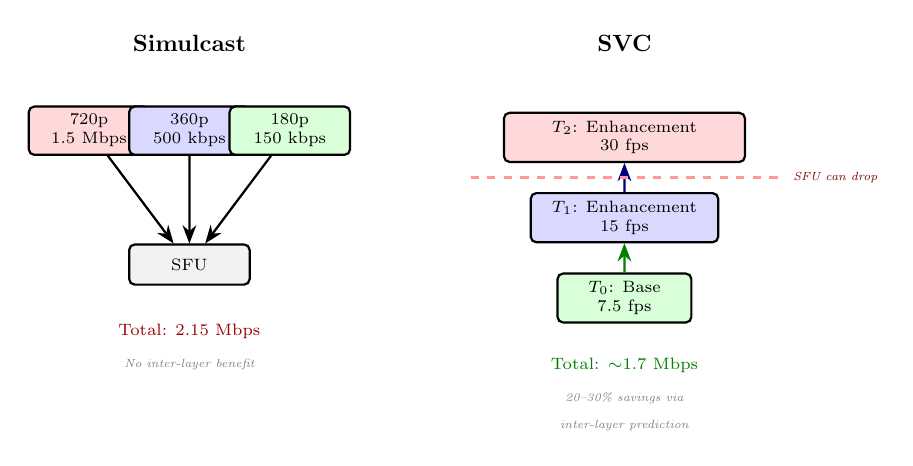
\begin{tikzpicture}[>=Stealth, scale=0.85, every node/.style={scale=0.85},
  layer/.style={draw, rounded corners=2pt, minimum width=1.8cm,
    minimum height=0.6cm, font=\scriptsize, align=center, thick}]

% --- Simulcast (left) ---
\node[font=\normalsize\bfseries] at (2, 5.8) {Simulcast};

% Three independent columns
\node[layer, fill=red!15] (s720) at (0.5, 4.5) {720p\\1.5 Mbps};
\node[layer, fill=blue!15] (s360) at (2.0, 4.5) {360p\\500 kbps};
\node[layer, fill=green!15] (s180) at (3.5, 4.5) {180p\\150 kbps};

\node[layer, fill=gray!10] (sfu1) at (2.0, 2.5) {SFU};

\draw[->, thick] (s720) -- (sfu1);
\draw[->, thick] (s360) -- (sfu1);
\draw[->, thick] (s180) -- (sfu1);

\node[font=\scriptsize, text=red!60!black] at (2.0, 1.5)
  {Total: 2.15 Mbps};
\node[font=\tiny\itshape, text=black!50] at (2.0, 1.0)
  {No inter-layer benefit};

% --- SVC (right) ---
\node[font=\normalsize\bfseries] at (8.5, 5.8) {SVC};

% Pyramid
\node[layer, fill=green!15, minimum width=2.0cm] (t0) at (8.5, 2.0)
  {$T_0$: Base\\7.5 fps};
\node[layer, fill=blue!15, minimum width=2.8cm] (t1) at (8.5, 3.2)
  {$T_1$: Enhancement\\15 fps};
\node[layer, fill=red!15, minimum width=3.6cm] (t2) at (8.5, 4.4)
  {$T_2$: Enhancement\\30 fps};

% Dependency arrows
\draw[->, thick, green!50!black] (t0) -- (t1);
\draw[->, thick, blue!50!black] (t1) -- (t2);

% Drop annotations
\draw[thick, dashed, red!40] (6.2, 3.8) -- (10.8, 3.8);
\node[font=\tiny\itshape, text=red!50!black, anchor=west] at (10.9, 3.8)
  {SFU can drop};

\node[font=\scriptsize, text=green!50!black] at (8.5, 1.0)
  {Total: ${\sim}$1.7 Mbps};
\node[font=\tiny\itshape, text=black!50] at (8.5, 0.5)
  {20--30\% savings via};
\node[font=\tiny\itshape, text=black!50] at (8.5, 0.1)
  {inter-layer prediction};

\end{tikzpicture}
\caption{Simulcast (left) encodes three independent bitstreams with no
  inter-layer compression. SVC (right) encodes a layered bitstream where
  temporal enhancement layers ($T_1$, $T_2$) reference the base layer
  ($T_0$), achieving 20--30\% savings. The SFU drops enhancement layers
  for bandwidth-constrained receivers.}
\label{fig:svc-architecture}
\end{figure}

Codec-specific SVC support relevant to WebRTC:

\begin{itemize}
\item \textbf{H.264 SVC (Annex~G).} Defines temporal, spatial, and quality
  scalability. Complex to implement; rarely used in WebRTC deployments.

\item \textbf{VP9 SVC.} Temporal scalability is widely deployed in WebRTC
  via libvpx (up to 3~temporal layers). Spatial SVC is defined but
  implementation-limited. VP9 temporal SVC is the primary mechanism
  enabling adaptive quality in Chrome/Firefox SFU-based calls.

\item \textbf{AV1 SVC.} Temporal scalability supported in both libaom and
  SVT-AV1. A key enabler for AV1 adoption in production WebRTC
  infrastructure, as SFUs require layered bitstreams to serve heterogeneous
  receivers.
\end{itemize}

Safari's lack of simulcast and SVC support in 2021 (Section~3.1) meant
that Safari users in multi-participant calls could not benefit from adaptive
quality---every receiver got the same stream regardless of bandwidth,
degrading the experience for all participants.

%% ---------------------------------------------------------------------------
\subsection{Hardware vs.\ Software Encoding}
\label{sec:hw-sw}

The main paper identifies hardware encoding as the deployment gate for
AV1 (Sections~8.5, 9.5). This section quantifies why.

\subsubsection{Encoding Complexity}

The computational cost of encoding a video frame is dominated by motion
estimation and RD-optimized mode decision. We express complexity as
operations per pixel:
\begin{equation}
  C_{\text{enc}} = C_{\text{ME}} + C_{\text{transform}}
    + C_{\text{quant}} + C_{\text{entropy}}
    + C_{\text{mode}}
  \label{eq:enc-complexity}
\end{equation}

Representative values for real-time presets:

\begin{itemize}
\item H.264 Constrained Baseline (``veryfast''): $C_{\text{enc}} \approx
  200$~ops/pixel
\item VP9 (speed~8, real-time): $C_{\text{enc}} \approx 600$~ops/pixel
\item AV1 (speed~10, real-time): $C_{\text{enc}} \approx 2000$~ops/pixel
\end{itemize}

The real-time constraint requires:
\begin{equation}
  C_{\text{enc}} \times W \times H \times \text{fps}
    \leq F_{\text{available}}
  \label{eq:realtime-constraint}
\end{equation}
where $F_{\text{available}}$ is the available computational throughput
(operations per second). For 720p/30fps AV1 at 2000~ops/pixel:
\begin{equation}
  2000 \times 921{,}600 \times 30 = 55.3 \times 10^9 \;\text{ops/s}
  \label{eq:av1-cost}
\end{equation}
This consumes approximately one full core of a modern desktop CPU. On
mobile devices with thermal and power constraints, software AV1 encoding
at 720p/30fps remains impractical without hardware acceleration.

\subsubsection{Hardware Encoder Architecture}

Hardware encoders implement a fixed subset of the codec's tool set in
dedicated silicon. The trade-off is quality for throughput: hardware
encoders typically produce output 10--20\% larger than software encoders
at equivalent visual quality because they implement fewer mode decision
candidates and simpler motion search:
\begin{equation}
  \Delta_{\text{HW}} \approx (1.1 \text{--} 1.2)
    \cdot \Delta_{\text{SW}}
  \label{eq:hw-quality-gap}
\end{equation}

This quality penalty is acceptable for real-time communication because:
(a)~the alternative---software encoding at a lower speed preset or reduced
resolution---incurs a larger quality penalty, and (b)~the freed CPU
capacity can be used for pre/post-processing, noise reduction, or
additional application logic.

\subsubsection{Hardware Encoder Availability}

\begin{table}[ht]
\centering
\small
\renewcommand{\arraystretch}{1.4}
\begin{tabularx}{\textwidth}{lXXXX}
\toprule
\textbf{Platform} & \textbf{H.264 HW} & \textbf{VP9 HW encode}
  & \textbf{AV1 HW encode} & \textbf{AV1 year} \\
\midrule
Intel (QSV) &
  Sandy Bridge+ (2011) &
  Kaby Lake+ (2017) &
  Arc / Meteor Lake+ &
  2022 \\
NVIDIA (NVENC) &
  Kepler+ (2012) &
  --- &
  Ada Lovelace+ &
  2022 \\
AMD (VCN) &
  VCN~1.0+ (2017) &
  --- &
  VCN~4.0+ (RDNA~3) &
  2023 \\
Apple (VideoToolbox) &
  A4+ (2010) &
  --- &
  M3+ &
  2023 \\
Qualcomm &
  SD~820+ (2016) &
  --- &
  SD~8 Gen~2+ &
  2023 \\
\bottomrule
\end{tabularx}
\caption{Hardware encoder availability timeline. H.264 hardware encoding
  has been ubiquitous for over a decade. AV1 hardware encoding began
  shipping in 2022--2023 across all major platforms; the main paper projects
  it becomes the practical WebRTC default by 2028--2030 as these chipsets
  reach market saturation.}
\label{tab:hw-encoders}
\end{table}

\excursus{Excursus: WebCodecs and hardware acceleration.}{When a WebCodecs
\texttt{VideoEncoder} is configured with \texttt{codec: "av01"}, the browser
selects hardware or software encoding based on platform capability and the
\texttt{hardwareAcceleration} preference (\texttt{"prefer-hardware"},
\texttt{"prefer-software"}, or \texttt{"no-preference"}). The application
receives encoded \texttt{EncodedVideoChunk} objects either way, but latency
and CPU cost differ dramatically: hardware encoding typically adds
$<\!1$~ms per frame and consumes near-zero CPU, while software AV1 at
real-time presets consumes an entire CPU core
(eq.~\ref{eq:av1-cost}). This abstraction is what makes the hardware
timeline in Table~\ref{tab:hw-encoders} directly relevant to the WebCodecs
adoption curve in Section~7.}

The hardware encoding timeline directly underpins the main paper's
projections: the ``AV1 becomes practical'' milestone (Section~8.5) and
``AV1 HW ubiquitous'' milestone (Section~9.5) depend on the chipset
generations in Table~\ref{tab:hw-encoders} reaching market saturation.

%% ---------------------------------------------------------------------------
\subsection{Implications for Real-Time Web Communication}
\label{sec:video-implications}

The DSP analysis of this appendix maps back to concrete implications for
the technologies surveyed in the main text.

\textbf{The hybrid coding framework is universal; innovation is
incremental.} Every codec from VP8 to VVC implements the same
prediction--transform--quantization--entropy framework
(Figure~\ref{fig:hybrid-encoder}). Generational improvements come from
expanding the tool set within this framework---more block sizes
(Table~\ref{tab:partitioning}), more prediction modes, more transform
types (Table~\ref{tab:transforms})---not from fundamentally new
architectures. This means the efficiency gap $\Delta$ approaches but never
reaches zero: each additional tool yields diminishing rate-distortion
improvement at increasing computational cost.

\textbf{Transform and prediction innovations explain the BD-Rate
progression.} The 35\% rate saving from H.264 to VP9 comes primarily from
larger blocks ($64\!\times\!64$ vs.\ $16\!\times\!16$) and adaptive
transforms (DCT$+$ADST vs.\ fixed DCT). The additional 30\% from VP9 to
AV1 comes from compound and warped motion, film grain synthesis, and
16-way transform type selection (Table~\ref{tab:bd-rate}). Each tool adds
encoding complexity proportional to its rate-distortion benefit, which is
why real-time encoders must aggressively prune the tool set.

\textbf{SVC is what makes multi-participant WebRTC work.} Without temporal
SVC, an SFU must forward full-rate streams to all participants regardless
of their bandwidth. With VP9/AV1 temporal SVC
(Section~\ref{sec:svc}), the SFU drops enhancement temporal layers for
bandwidth-constrained receivers, degrading frame rate gracefully while
preserving spatial quality. The 20--30\% savings over simulcast
(eq.~\ref{eq:svc-advantage}) translate directly to reduced server egress
bandwidth in large meetings.

\textbf{Hardware encoding is the deployment gate, not codec specification.}
AV1 was specified in 2018 but becomes a practical WebRTC default only
when hardware encoders are ubiquitous (${\sim}$2028--2030). The DSP tools
that make AV1 efficient---warped motion, OBMC, $128\!\times\!128$
superblocks with flexible partitioning---are precisely the tools that make
it computationally expensive in software (eq.~\ref{eq:av1-cost}). The
${\sim}$10--20\% quality penalty of hardware encoders
(eq.~\ref{eq:hw-quality-gap}) is the price of real-time feasibility, and
it is a price worth paying: $\Delta_{\text{AV1,HW}} \approx 0.6$ is still
far below $\Delta_{\text{VP9,SW}} \approx 0.8$.

\textbf{The convergence toward Shannon is real but asymptotic.}
Cross-referencing with Appendix~\ref{app:info-theory}: H.264's
$\Delta \approx 2.1$ means it operates at $3.1\times$ the theoretical
minimum rate. VP9's $\Delta \approx 0.8$ means $1.8\times$. AV1's
$\Delta \approx 0.5$ means $1.5\times$. VVC's $\Delta \approx 0.3$ means
$1.3\times$. Each generation captures more spatial, temporal, and
perceptual redundancy, but the returns are diminishing: the distance from
H.264 to VP9 ($-$35\%) exceeds VP9 to AV1 ($-$30\%), which exceeds AV1 to
VVC ($-$17\%). The next generation of efficiency gains for real-time web
communication will come not from codecs alone, but from the co-optimization
of transport (QUIC, WebTransport), application architecture (WebCodecs,
unbundled pipelines), and network infrastructure that the main text
describes.

%
% Requires in the preamble: amsmath, amssymb, tabularx, booktabs

\section{Video Compression Fundamentals}
\label{app:video-compression}

Appendix~\ref{app:info-theory} quantified the coding efficiency gap $\Delta$
(eq.~\ref{eq:coding-gap}) for each codec generation, treating codecs as black
boxes characterized by their distance from the Shannon rate-distortion bound.
This appendix opens those black boxes. We examine the signal processing and
coding techniques that determine $\Delta$: how video codecs exploit spatial,
temporal, and perceptual redundancy, what distinguishes one codec generation
from the next, and why computational complexity---not algorithmic
capability---remains the binding constraint for real-time web communication.

%% ---------------------------------------------------------------------------
\subsection{Why Video Is Compressible}
\label{sec:compressible}

A raw digital video signal carries far more data than information. Three
fundamental redundancies make compression ratios of 200:1 to 500:1 achievable
at perceptually acceptable quality.

\subsubsection{Spatial Redundancy}

Natural images exhibit strong local correlation. The autocorrelation function
for a typical image row can be modeled as a first-order Markov process:
\begin{equation}
  R_{xx}(k) = \sigma^2 \rho^{|k|}
  \label{eq:spatial-autocorr}
\end{equation}
where $\sigma^2$ is the pixel variance and $\rho \in [0.90, 0.97]$ for
natural content. The separable two-dimensional extension is:
\begin{equation}
  R_{xx}(k, l) = \sigma^2 \,\rho_h^{|k|}\, \rho_v^{|l|}
  \label{eq:spatial-autocorr-2d}
\end{equation}
The power spectral density---the Fourier transform of
(\ref{eq:spatial-autocorr-2d})---is concentrated at low spatial frequencies,
meaning most of the signal energy occupies a small fraction of the frequency
domain. This concentration is the foundation of transform coding
(Section~\ref{sec:transforms}).

\subsubsection{Temporal Redundancy}

Consecutive video frames are highly correlated. For typical conversational
video at 30~fps, the inter-frame correlation coefficient is:
\begin{equation}
  \text{Corr}(f_t, f_{t-1}) \approx 0.90\text{--}0.98
  \label{eq:temporal-corr}
\end{equation}
Most pixels change little between frames; only regions containing motion,
lighting changes, or scene cuts carry significant new information. Motion
estimation (Section~\ref{sec:motion}) exploits this by predicting each block
from a displaced version of a reference frame, transmitting only the
prediction residual.

\subsubsection{Perceptual Irrelevance}

The human visual system (HVS) has lower spatial acuity for chrominance than
luminance. This asymmetry motivates \emph{chroma subsampling}: representing
color difference channels at reduced resolution relative to the luma channel.

\excursus{Excursus: Why 4:2:0?}{All WebRTC codecs operate on YCbCr 4:2:0
video, where each chroma channel is sampled at half the horizontal and half
the vertical resolution of luma. This reduces the sample count by a factor of
$1 + 0.25 + 0.25 = 1.5$ relative to $1 + 1 + 1 = 3$ for full-resolution
4:4:4 color, a 2$\times$ saving before any coding begins. Perceptual
experiments confirm that 4:2:0 is essentially indistinguishable from 4:4:4 at
typical viewing distances for video conferencing---the HVS cannot resolve
the missing chroma detail.}

\subsubsection{The Compression Imperative}

A raw 720p/30fps 4:2:0 video stream at 8~bits per sample requires:
\begin{equation}
  R_{\text{raw}} = 1280 \times 720 \times 1.5 \times 8 \times 30
    = 331.8 \;\text{Mbps}
  \label{eq:raw-rate}
\end{equation}
This exceeds the 120~Mbps median link capacity cited in
Table~\ref{tab:inet}. The Shannon rate-distortion bound
(eq.~\ref{eq:rate-distortion}) yields approximately 0.7--1.5~Mbps at
perceptually acceptable distortion---a compression ratio of 220:1 to 475:1.
Video compression is not optional for real-time communication; it is a
prerequisite.

The first-order entropy of raw pixel values $H(X)$ greatly exceeds the
conditional entropy given neighboring samples:
\begin{equation}
  H(X) \gg H(X \mid X_{\text{neighbors}})
  \label{eq:conditional-entropy}
\end{equation}
This gap---the mutual information between a pixel and its
neighbors---represents the exploitable redundancy. The entire hybrid coding
framework (Section~\ref{sec:hybrid}) is designed to extract this mutual
information through prediction, leaving only the irreducible residual for
transform coding and quantization.

%% ---------------------------------------------------------------------------
\subsection{The Hybrid Coding Framework}
\label{sec:hybrid}

Every major video codec since H.261 (1988)---including every codec in the
WebRTC stack---is a variation on the \emph{block-based hybrid coding}
framework. The encoder partitions each frame into blocks, predicts each block
from previously coded data, transforms and quantizes the prediction residual,
and entropy codes the result.

\subsubsection{Encoder Signal Flow}

For a block at position $(x,y)$ in frame $f_t$, the encoder computes a
prediction $\hat{f}_{\text{pred}}(x,y)$ from either the current frame
(intra prediction) or a reference frame (inter prediction). The prediction
residual is:
\begin{equation}
  e(x,y) = f_t(x,y) - \hat{f}_{\text{pred}}(x,y)
  \label{eq:residual}
\end{equation}
The residual is transformed, quantized, and entropy coded to produce the
bitstream. The decoder reconstructs the frame as:
\begin{equation}
  \hat{f}(x,y) = \hat{e}(x,y) + \hat{f}_{\text{pred}}(x,y)
  \label{eq:reconstruction}
\end{equation}
where $\hat{e}$ is the inverse-transformed, dequantized residual.

\subsubsection{Rate-Distortion Optimization}

Every coding decision---block partition, prediction mode, motion vector,
transform type, quantization level---is made by minimizing a Lagrangian
rate-distortion cost:
\begin{equation}
  J(m) = D(m) + \lambda \cdot R(m)
  \label{eq:rd-cost}
\end{equation}
where $m \in \mathcal{M}$ is a coding mode, $D(m)$ is the distortion
(typically sum of squared errors), $R(m)$ is the bit cost, and $\lambda$ is a
Lagrange multiplier controlling the rate-distortion trade-off. The optimal
mode satisfies:
\begin{equation}
  m^* = \arg\min_{m \in \mathcal{M}} \left[ D(m) + \lambda \cdot R(m) \right]
  \label{eq:rd-opt}
\end{equation}
The Lagrange multiplier relates to the quantization parameter (QP) via an
empirically validated exponential relationship:
\begin{equation}
  \lambda = c \cdot 2^{(QP - 12)/3}
  \label{eq:lambda-qp}
\end{equation}
where $c$ is a codec-specific constant. This relationship ensures that
finer quantization (lower QP) assigns higher cost to bits, favoring modes
that reduce distortion, while coarser quantization (higher QP) favors
modes that reduce rate.

\begin{figure}[ht]
\centering
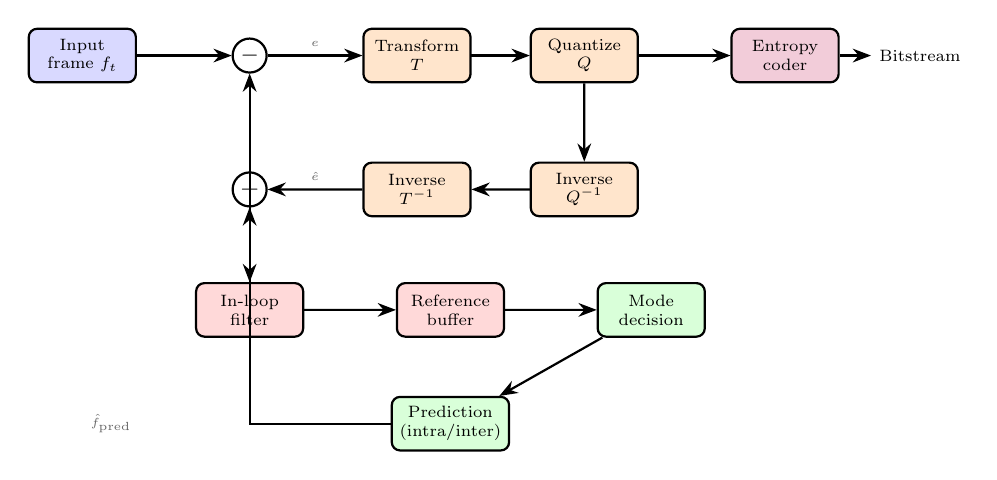
\begin{tikzpicture}[>=Stealth, scale=0.85, every node/.style={scale=0.85},
  block/.style={draw, rounded corners=3pt, minimum width=1.6cm,
    minimum height=0.8cm, font=\scriptsize, align=center, thick},
  arrow/.style={->, thick},
  label/.style={font=\tiny, text=black!60}]

% --- Input ---
\node[block, fill=blue!15] (input) at (0, 0) {Input\\frame $f_t$};

% --- Subtract ---
\node[draw, circle, inner sep=1.5pt, thick] (sub) at (2.5, 0) {$-$};

% --- Transform ---
\node[block, fill=orange!20] (transform) at (5, 0) {Transform\\$T$};

% --- Quantize ---
\node[block, fill=orange!20] (quant) at (7.5, 0) {Quantize\\$Q$};

% --- Entropy ---
\node[block, fill=purple!20] (entropy) at (10.5, 0) {Entropy\\coder};

% --- Bitstream ---
\node[font=\scriptsize, right=0.4cm of entropy] (bitstream) {Bitstream};

% --- Inverse Quantize ---
\node[block, fill=orange!20] (iquant) at (7.5, -2) {Inverse\\$Q^{-1}$};

% --- Inverse Transform ---
\node[block, fill=orange!20] (itransform) at (5, -2) {Inverse\\$T^{-1}$};

% --- Add ---
\node[draw, circle, inner sep=1.5pt, thick] (add) at (2.5, -2) {$+$};

% --- In-loop filter ---
\node[block, fill=red!15] (filter) at (2.5, -3.8) {In-loop\\filter};

% --- Reference buffer ---
\node[block, fill=red!15] (refbuf) at (5.5, -3.8) {Reference\\buffer};

% --- Mode decision ---
\node[block, fill=green!15] (mode) at (8.5, -3.8) {Mode\\decision};

% --- Prediction ---
\node[block, fill=green!15] (pred) at (5.5, -5.5) {Prediction\\(intra/inter)};

% --- Forward path ---
\draw[arrow] (input) -- (sub);
\draw[arrow] (sub) -- node[above, label] {$e$} (transform);
\draw[arrow] (transform) -- (quant);
\draw[arrow] (quant) -- (entropy);
\draw[arrow] (entropy) -- (bitstream);

% --- Reconstruction path ---
\draw[arrow] (quant) -- (iquant);
\draw[arrow] (iquant) -- (itransform);
\draw[arrow] (itransform) -- node[above, label] {$\hat{e}$} (add);

% --- Filter and buffer ---
\draw[arrow] (add) -- (filter);
\draw[arrow] (filter) -- (refbuf);

% --- Prediction feedback ---
\draw[arrow] (refbuf) -- (mode);
\draw[arrow] (mode) -- (pred);
\draw[arrow] (pred) -| (sub);
\draw[arrow] (pred) -| (add);

% --- Labels ---
\node[label, anchor=west] at (0, -5.5) {$\hat{f}_{\text{pred}}$};

\end{tikzpicture}
\caption{Block-based hybrid encoder architecture. Every codec from H.264
  through VVC follows this structure: predict each block from previously
  coded data (green), transform and quantize the residual (orange), entropy
  code the result (purple), then reconstruct and filter for future
  reference (red). The coding efficiency gap $\Delta$
  (eq.~\ref{eq:coding-gap}) arises from sub-optimal prediction, imperfect
  energy compaction, quantization beyond the rate-distortion bound, and
  entropy coding overhead.}
\label{fig:hybrid-encoder}
\end{figure}

The four sub-optimal components of Figure~\ref{fig:hybrid-encoder}---prediction,
transform, quantization, and entropy coding---each contribute to $\Delta$:
\begin{equation}
  \Delta \approx \Delta_{\text{pred}} + \Delta_{\text{transform}}
    + \Delta_{\text{quant}} + \Delta_{\text{entropy}}
  \label{eq:delta-decomp}
\end{equation}
Generational codec improvements reduce one or more of these terms. The codec
lineages in Sections~\ref{sec:mpeg-lineage}--\ref{sec:aom-lineage} trace
exactly which tools target which terms.

%% ---------------------------------------------------------------------------
\subsection{Transforms}
\label{sec:transforms}

The transform stage decorrelates the prediction residual, concentrating
energy into a few coefficients that can be efficiently quantized and coded.

\subsubsection{The KLT and Its DCT Approximation}
\label{sec:klt-dct}

The optimal decorrelating transform for a stationary source is the
\emph{Karhunen-Lo\`eve Transform} (KLT), whose basis vectors are the
eigenvectors of the input autocorrelation matrix $\mathbf{R}_{xx}$. For a
first-order Markov source with correlation $\rho$ (eq.~\ref{eq:spatial-autocorr}),
the KLT basis converges to the Type-II DCT as block size grows:
\begin{equation}
  C_k(n) = \alpha_k \cos\!\left[\frac{\pi k (2n+1)}{2N}\right],
  \quad k,n = 0, \ldots, N-1
  \label{eq:dct-ii}
\end{equation}
where $\alpha_0 = \sqrt{1/N}$ and $\alpha_k = \sqrt{2/N}$ for $k > 0$.

The energy compaction efficiency---the fraction of total energy captured by
the first $K$ of $N$ coefficients---is:
\begin{equation}
  \eta(K, N) = \frac{\sum_{k=0}^{K-1} \sigma_k^2}
    {\sum_{k=0}^{N-1} \sigma_k^2}
  \label{eq:energy-compaction}
\end{equation}
where $\sigma_k^2$ is the variance of the $k$-th transform coefficient.
For a typical intra residual with $\rho = 0.95$ and $N = 8$, the first 3
DCT coefficients capture approximately 95\% of the energy. This
concentration enables aggressive quantization of high-frequency coefficients
with minimal perceptual impact.

\subsubsection{Integer Transforms in Practice}
\label{sec:integer-transforms}

Practical codecs use integer approximations of the DCT to ensure bit-exact
encoder-decoder agreement. H.264 introduced a $4 \times 4$ integer
transform:
\begin{equation}
  \mathbf{H}_4 = \begin{pmatrix}
    1 &  1 &  1 &  1 \\
    2 &  1 & -1 & -2 \\
    1 & -1 & -1 &  1 \\
    1 & -2 &  2 & -1
  \end{pmatrix}
  \label{eq:h264-transform}
\end{equation}
The non-unity scaling factors are absorbed into the quantization step,
preserving exact integer arithmetic throughout the encode-decode loop.

Each codec generation expands the transform toolkit:

\begin{table}[ht]
\centering
\small
\renewcommand{\arraystretch}{1.4}
\begin{tabularx}{\textwidth}{lXXX}
\toprule
\textbf{Codec} & \textbf{Transform sizes} & \textbf{Transform types}
  & \textbf{Selection method} \\
\midrule
H.264 &
  $4\!\times\!4$, $8\!\times\!8$ &
  Integer DCT &
  Fixed per block size \\
VP9 &
  $4\!\times\!4$ to $32\!\times\!32$ &
  DCT, ADST &
  Row/column adaptive \\
HEVC &
  $4\!\times\!4$ to $32\!\times\!32$ &
  Integer DCT, DST ($4\!\times\!4$ intra) &
  Mode-dependent \\
AV1 &
  $4\!\times\!4$ to $64\!\times\!64$ &
  DCT, ADST, FlipADST, Identity &
  RD-optimized per block \\
VVC &
  $4\!\times\!4$ to $64\!\times\!64$ &
  DCT-II, DST-VII $+$ LFNST &
  RD-optimized $+$ secondary \\
\bottomrule
\end{tabularx}
\caption{Transform sizes and types across codec generations. AV1 applies
  four 1D transform types independently to rows and columns, yielding
  16~possible 2D combinations per block. VVC adds a non-separable secondary
  transform (LFNST) applied to low-frequency coefficients after the primary
  separable transform.}
\label{tab:transforms}
\end{table}

The Asymmetric Discrete Sine Transform (ADST) used in VP9 and AV1 is
particularly effective for intra-predicted residuals, which tend to have
larger magnitudes near the prediction boundary. AV1's FlipADST extends
this to blocks where the large residuals are on the opposite edge, while
the Identity transform (skip) handles blocks where the residual is already
well-distributed in the spatial domain.

The progression from fixed transforms (H.264) to RD-optimized multi-type
selection (AV1, VVC) directly reduces $\Delta_{\text{transform}}$ in
(\ref{eq:delta-decomp}): better energy compaction means fewer bits are
needed to represent the same residual at a given distortion level.

%% ---------------------------------------------------------------------------
\subsection{Motion Estimation and Inter Prediction}
\label{sec:motion}

Inter prediction exploits temporal redundancy by predicting blocks in the
current frame from previously coded reference frames. This is the single
largest source of compression gain---the prediction residual
(eq.~\ref{eq:residual}) typically has 10--20$\times$ less energy than the
original signal.

\subsubsection{Block Matching and Motion Vectors}
\label{sec:block-matching}

The encoder searches for the best-matching region in a reference frame by
minimizing a cost function over candidate displacement vectors
$\mathbf{d} = (d_x, d_y)$:
\begin{equation}
  \text{SAD}(\mathbf{d}) = \sum_{(x,y) \in B}
    \left| f_t(x,y) - f_{t-1}(x + d_x,\, y + d_y) \right|
  \label{eq:sad}
\end{equation}
The Sum of Absolute Differences (SAD) is the simplest distortion measure.
A better rate-distortion proxy is the Sum of Absolute Transformed
Differences (SATD), which applies the Hadamard transform before summation:
\begin{equation}
  \text{SATD}(\mathbf{d}) = \sum \left| \mathbf{H}
    \cdot \left( f_t - f_{t-1}(\mathbf{d}) \right) \right|
  \label{eq:satd}
\end{equation}
SATD approximates the post-transform energy and thus better predicts the
actual coded bit cost. Rate-constrained motion estimation augments the
distortion with a motion vector coding cost:
\begin{equation}
  \mathbf{d}^* = \arg\min_{\mathbf{d}} \left[
    \text{SATD}(\mathbf{d}) + \lambda_{\text{motion}} \cdot R(\mathbf{d})
  \right]
  \label{eq:rcme}
\end{equation}
where $R(\mathbf{d})$ is the bit cost of encoding the motion vector
relative to a predictor.

\subsubsection{Sub-Pixel Interpolation}
\label{sec:subpixel}

Motion in natural video rarely aligns to integer pixel positions. All modern
codecs perform sub-pixel motion compensation by interpolating reference
frame samples at fractional positions.

H.264 uses a 6-tap filter for half-pixel luma interpolation:
\begin{equation}
  h_{\frac{1}{2}} = \{1, -5, 20, 20, -5, 1\} / 32
  \label{eq:h264-halfpel}
\end{equation}
with quarter-pixel positions obtained by bilinear averaging of integer and
half-pixel samples. HEVC extends this to an 8-tap filter for half-pixel and
a 7-tap filter for quarter-pixel positions. AV1 introduces a switchable
filter bank with three 8-tap options---Regular (sharp), Smooth (low-pass),
and Sharp (high-frequency preserving)---selected per block via RD
optimization. VVC adds DMVR (Decoder-side Motion Vector Refinement) and
BDOF (Bi-Directional Optical Flow) for sub-pixel refinement at the decoder
without additional signaling bits.

The progression from H.264's fixed 6-tap filter to AV1's switchable bank
reduces $\Delta_{\text{pred}}$: better interpolation means smaller
prediction residuals, which require fewer bits.

\subsubsection{Advanced Inter Prediction Tools}
\label{sec:advanced-inter}

Beyond basic block matching, each codec generation adds tools to handle
complex motion and occlusion:

\begin{itemize}
\item \textbf{Multiple reference frames.} H.264 introduced up to 16
  reference frames; practical WebRTC encoders use 1--3 for latency reasons.
  More references improve prediction for periodic motion and uncovered
  backgrounds.

\item \textbf{Bi-prediction.} A weighted average of predictions from two
  reference frames, reducing noise and handling gradual scene changes.
  Available from H.264 onward (in B-frames) and in AV1's compound modes.

\item \textbf{Compound prediction (AV1).} Wedge masks and
  difference-weighted blending combine two predictions at the block level,
  handling occlusion boundaries where a single motion model fails.

\item \textbf{Overlapped Block Motion Compensation (AV1).} Blends
  predictions from neighboring blocks at motion boundaries, reducing
  blocking artifacts without post-processing.

\item \textbf{Warped motion (AV1).} An affine model with up to 6
  parameters handles rotation, zoom, and perspective---common in
  screen sharing and camera motion.

\item \textbf{VVC additions.} Geometric Partitioning Mode (non-rectangular
  block splits for motion boundaries), BDOF (optical flow refinement at the
  decoder), and DMVR (decoder-side MV refinement using bilateral matching).
\end{itemize}

\excursus{Excursus: Motion estimation in real-time encoding.}{Full-search
block matching has complexity $O(N^2 \cdot S^2)$ where $N$ is the block
dimension and $S$ is the search range in pixels. For a $64\!\times\!64$
block with $S = 64$, this is ${\sim}17$ million SAD operations per
block---far too expensive for real-time encoding. WebRTC encoders use
hierarchical search patterns (diamond, hexagon) that reduce complexity to
$O(N^2 \cdot \log S)$ with typically $< 5\%$ rate-distortion penalty
relative to full search. This is why real-time encoders use only a subset
of each codec's inter prediction tools: the full tool set is available
for offline encoding, but the real-time constraint forces aggressive
pruning of the mode decision search space.}

%% ---------------------------------------------------------------------------
\subsection{Quantization}
\label{sec:quantization}

Quantization is the sole lossy step in the hybrid coding pipeline. It maps
continuous-valued (or high-precision integer) transform coefficients to a
discrete set of reconstruction levels, introducing controlled information
loss to achieve the target bit rate.

\subsubsection{Scalar Quantization}

Uniform scalar quantization maps coefficient $c$ to a quantization index:
\begin{equation}
  q = \text{round}\!\left(\frac{c}{Q_{\text{step}}}\right), \quad
  \hat{c} = q \cdot Q_{\text{step}}
  \label{eq:uniform-quant}
\end{equation}
Modern codecs use \emph{dead-zone quantization}, where coefficients near
zero are mapped to zero more aggressively than uniform rounding predicts:
\begin{equation}
  q = \text{sign}(c) \cdot \left\lfloor
    \frac{|c| - f \cdot Q_{\text{step}}}{Q_{\text{step}}}
  \right\rfloor
  \label{eq:deadzone}
\end{equation}
where $f \in [0, 0.5)$ controls the dead-zone width. Dead-zone
quantization increases sparsity---the fraction of zero-valued
coefficients---which dramatically improves entropy coding efficiency.

\subsubsection{QP-to-Step-Size Mapping}

The quantization parameter (QP) controls the step size via an exponential
relationship. In the H.264/HEVC/VVC family:
\begin{equation}
  Q_{\text{step}} = Q_0 \cdot 2^{(QP - QP_0)/6}
  \label{eq:qp-mapping}
\end{equation}
A 6-unit increase in QP doubles the step size, approximately doubling the
bit rate. AV1 uses a similar but codec-specific mapping with separate QP
values for DC and AC coefficients, plus per-segment QP adjustment for
region-of-interest coding.

\subsubsection{Quantization Distortion}

For a single coefficient under uniform quantization at high rate, the
distortion is:
\begin{equation}
  D_q = \frac{Q_{\text{step}}^2}{12}
  \label{eq:quant-distortion}
\end{equation}
For a block of $N$ transform coefficients where $K$ survive quantization
(nonzero) and $N - K$ are quantized to zero:
\begin{equation}
  D_{\text{block}} \approx K \cdot \frac{Q_{\text{step}}^2}{12}
    + \sum_{k \notin K} c_k^2
  \label{eq:block-distortion}
\end{equation}
The second term represents the energy of coefficients eliminated by the
dead zone---information permanently discarded. The QP is thus the primary
control knob for navigating the rate-distortion curve in
Figure~\ref{fig:rate-distortion}. The WebCodecs \texttt{VideoEncoder} API
exposes this control via the \texttt{quantizer} configuration parameter,
giving JavaScript applications direct access to this fundamental
trade-off.

%% ---------------------------------------------------------------------------
\subsection{Entropy Coding}
\label{sec:entropy-coding}

After quantization, the surviving coefficients and all side information
(motion vectors, prediction modes, block partitions) must be losslessly
compressed. The entropy coder converts these symbols into a bitstream,
approaching the conditional entropy $H(X|\text{context})$ as closely as
possible. The gap between the entropy coder's output rate and the true
conditional entropy is $\Delta_{\text{entropy}}$ in
(\ref{eq:delta-decomp}).

\subsubsection{Context-Adaptive Binary Arithmetic Coding (CABAC)}
\label{sec:cabac}

CABAC, used in H.264, HEVC, and VVC, encodes each syntax element as a
sequence of binary decisions (bins). For each bin, the arithmetic coder
subdivides the current interval $[L, H)$ based on the estimated
probability $p$:
\begin{equation}
  [L, H) \to \begin{cases}
    [L,\; L + p \cdot (H - L)) & \text{if bin} = 0 \\
    [L + p \cdot (H - L),\; H) & \text{if bin} = 1
  \end{cases}
  \label{eq:arithmetic-coding}
\end{equation}
The theoretical output length approaches the entropy:
\begin{equation}
  \ell \to \sum_{i=1}^{n} -\log_2 p(b_i \mid \text{ctx}_i)
  \label{eq:cabac-length}
\end{equation}
CABAC achieves redundancy below 0.01 bits/symbol relative to the true
conditional entropy---near-optimal compression.

Context modeling is the key to CABAC's effectiveness. Each bin type has an
associated context, whose probability is updated after each observation via
a state-machine-based exponential moving average:
\begin{equation}
  p_{k+1} = p_k + \alpha(s_k) \cdot (b_k - p_k)
  \label{eq:cabac-update}
\end{equation}
where $\alpha(s_k)$ is a state-dependent adaptation rate, indexed by a
lookup table with 64 states (H.264) or 128 states (HEVC/VVC). This design
avoids floating-point arithmetic entirely.

CABAC also provides a \emph{bypass mode} for bins with approximately
uniform probability (e.g., sign bits, high-magnitude coefficient levels),
which skips the context lookup and probability estimation for throughput.

\subsubsection{Multi-Symbol Arithmetic Coding in AV1}
\label{sec:av1-entropy}

AV1 departs from binary arithmetic coding. Its entropy coder operates on
multi-symbol alphabets using CDF (Cumulative Distribution Function) tables:
\begin{equation}
  \text{Encode symbol } s: \quad
  [L, H) \to \left[L + \frac{\text{CDF}(s-1)}{M} \cdot (H-L),\;
    L + \frac{\text{CDF}(s)}{M} \cdot (H-L)\right)
  \label{eq:av1-entropy}
\end{equation}
where $M$ is the total frequency count. CDF tables are adapted after
each symbol:
\begin{equation}
  \text{CDF}_{k+1}(s) = \text{CDF}_k(s) + \left\lfloor
    \frac{\text{target}(s) - \text{CDF}_k(s)}{n}
  \right\rfloor
  \label{eq:cdf-update}
\end{equation}
where $n$ controls the adaptation rate. Multi-symbol coding is more
efficient than CABAC's binarization for syntax elements with moderate
alphabet sizes (e.g., intra prediction modes, transform types), as it
avoids the overhead of converting each symbol into a binary tree of
decisions.

\begin{table}[ht]
\centering
\small
\renewcommand{\arraystretch}{1.4}
\begin{tabularx}{\textwidth}{lXXXXX}
\toprule
\textbf{Feature} & \textbf{H.264} & \textbf{HEVC} & \textbf{VP9}
  & \textbf{AV1} & \textbf{VVC} \\
\midrule
Method &
  Binary AC &
  Binary AC &
  Boolean AC &
  Multi-sym AC &
  Binary AC \\
Contexts &
  ${\sim}400$ &
  ${\sim}200$ &
  ${\sim}900$ &
  ${\sim}300$ &
  ${\sim}700$ \\
Adaptation &
  64-state LUT &
  128-state LUT &
  Counter &
  CDF update &
  128-state LUT \\
Bypass mode &
  Yes &
  Yes &
  N/A &
  N/A &
  Yes \\
Parallelism &
  Slice &
  WPP / Tiles &
  Tiles &
  Tiles &
  WPP / Tiles \\
\bottomrule
\end{tabularx}
\caption{Entropy coding comparison across codecs. HEVC reduced context
  count relative to H.264 for throughput; VVC increased it again for
  improved compression. AV1's multi-symbol approach operates on full
  alphabets rather than binary decompositions.}
\label{tab:entropy-coding}
\end{table}

The frame entropy $\hat{H}(f_t)$ from eq.~(\ref{eq:frame-entropy}) is
ultimately determined by how well the entropy coder's probability model
matches the true symbol distribution. Both CABAC and AV1's multi-symbol
coder achieve near-zero entropy coding gaps; the remaining
$\Delta_{\text{entropy}}$ arises primarily from context model mismatch on
non-stationary content (scene changes, sudden motion onset).

%% ---------------------------------------------------------------------------
\subsection{In-Loop Filtering}
\label{sec:filtering}

Block-based coding introduces visible artifacts at block boundaries:
discontinuities from independent quantization of adjacent blocks, and
ringing from coefficient truncation. In-loop filters reduce these artifacts
\emph{before} the reconstructed frame enters the reference buffer, improving
prediction quality for subsequent frames and thus reducing
$\Delta_{\text{pred}}$.

\begin{itemize}
\item \textbf{Deblocking filter (all codecs).} Smooths discontinuities
  at block edges, with filter strength adapted to the quantization level
  and local gradient. Introduced in H.264; refined in each subsequent
  codec.

\item \textbf{Sample Adaptive Offset---SAO (HEVC).} Classifies
  reconstructed samples by intensity or edge direction and applies
  per-class offsets to reduce systematic bias introduced by quantization.

\item \textbf{Constrained Directional Enhancement Filter---CDEF (AV1).}
  A directional filter that identifies edge orientation per
  $8\!\times\!8$ block and applies filtering only along the edge,
  preserving sharpness while reducing ringing.

\item \textbf{Loop Restoration Filter (AV1).} A switchable per-tile
  filter choosing between a Wiener filter (FIR designed to minimize MSE
  between original and reconstruction) and a Self-Guided filter (non-linear
  denoising based on guided image filtering). This is AV1's most powerful
  quality enhancement tool.

\item \textbf{Adaptive Loop Filter---ALF (VVC).} A diamond-shaped filter
  with coefficients signaled per frame, applied adaptively per
  $4\!\times\!4$ block based on local classification. Subsumes HEVC's
  SAO functionality.
\end{itemize}

The evolution from simple deblocking (H.264) to multi-stage adaptive
filtering (AV1: deblocking $\to$ CDEF $\to$ loop restoration) exemplifies
how each codec generation reduces $\Delta_{\text{pred}}$ by improving
reference frame quality.

%% ---------------------------------------------------------------------------
\subsection{Codec Lineage: MPEG/ITU Family}
\label{sec:mpeg-lineage}

The MPEG/ITU standardization track has produced three codec generations
relevant to the 2021--2031 timeframe of this document.

\subsubsection{H.264/AVC (2003)}
\label{sec:h264}

H.264 defined the modern era of video compression and remains the most
widely deployed codec. Its key innovations over its predecessors (H.263,
MPEG-2):

\begin{itemize}
\item Variable block sizes: $16\!\times\!16$ macroblock partitioned into
  $16\!\times\!8$, $8\!\times\!16$, $8\!\times\!8$, $8\!\times\!4$,
  $4\!\times\!8$, and $4\!\times\!4$ sub-partitions for motion
  compensation.

\item Quarter-pixel motion compensation with 6-tap interpolation
  (eq.~\ref{eq:h264-halfpel}).

\item Context-adaptive intra prediction: 9~angular modes for
  $4\!\times\!4$ blocks, 4~modes for $16\!\times\!16$.

\item Dual entropy coding: CAVLC (simpler, faster) and CABAC
  (Section~\ref{sec:cabac}; 10--15\% better compression).

\item In-loop deblocking filter, mandatory for the decoder.

\item Multiple reference frames (up to 16) and weighted prediction.
\end{itemize}

Three profiles are relevant to WebRTC: \textbf{Constrained Baseline}
(no CABAC, no B-frames, lowest complexity---the mandatory WebRTC profile),
\textbf{Main} (CABAC, B-frames, ${\sim}$10\% better compression), and
\textbf{High} ($8\!\times\!8$ transform, adaptive quantization matrices,
${\sim}$15\% better).

At the 720p/30fps reference point, H.264 Constrained Baseline operates at
approximately 2.0--2.5~Mbps for ``good'' quality (PSNR ${\sim}$37~dB),
corresponding to $\Delta_{\text{H.264}} \approx 2.1$ from
Appendix~\ref{app:info-theory}. H.264 was the only codec Safari supported
in 2021 (Section~3.1), and its higher $\Delta$ is directly responsible
for the bandwidth disparity between Safari-only and VP9-capable sessions
documented in the main text.

\subsubsection{H.265/HEVC (2013)}
\label{sec:hevc}

HEVC replaced H.264's fixed $16\!\times\!16$ macroblock with a recursive
Coding Tree Unit (CTU) of up to $64\!\times\!64$ pixels, using quad-tree
partitioning down to $8\!\times\!8$. Key advances:

\begin{itemize}
\item 35 intra prediction angular directions (vs.\ H.264's 9).
\item Transform sizes from $4\!\times\!4$ to $32\!\times\!32$, with
  DST for $4\!\times\!4$ intra blocks.
\item Advanced Motion Vector Prediction (AMVP): two MVP candidates selected
  from spatial and temporal neighbors, replacing H.264's less structured
  motion vector prediction.
\item Merge mode: inherits the full motion information (MV, reference
  index, prediction direction) from a neighboring block, requiring zero
  additional motion bits.
\item Sample Adaptive Offset (SAO) in-loop filter.
\item Parallel processing: Wavefront Parallel Processing (WPP) and tiles.
\end{itemize}

HEVC achieves approximately 40\% rate reduction over H.264 at equivalent
PSNR. However, HEVC is absent from WebRTC entirely---not due to technical
limitations, but due to patent licensing.

\excursus{Excursus: Why no HEVC in WebRTC?}{HEVC's patent licensing is
fragmented across three separate pools (MPEG-LA, HEVC Advance, Velos Media)
plus independent licensors who are not members of any pool. The resulting
uncertainty about total royalty cost---estimated at \$0.20--\$0.40 per device
for some use cases---led Google, Mozilla, Cisco, and others to form the
Alliance for Open Media (AOM) in 2015 and develop AV1 as a royalty-free
alternative. This patent-driven fork is why the WebRTC ecosystem followed the
VP8$\to$VP9$\to$AV1 path rather than H.264$\to$HEVC$\to$VVC, and why the two
codec families must be understood in parallel.}

\subsubsection{H.266/VVC (2020)}
\label{sec:vvc}

VVC extends HEVC's quad-tree with binary and ternary splits, creating a
\emph{multi-type tree} (MTT) that enables asymmetric block shapes (e.g.,
$32\!\times\!8$, $8\!\times\!32$, $32\!\times\!4$). Additional
innovations:

\begin{itemize}
\item 67 intra prediction directions plus Matrix-based Intra Prediction
  (MIP), which applies a learned linear transform to neighboring samples.

\item Multiple Transform Selection (MTS): explicit signaling of DCT-II or
  DST-VII per block, plus the Low-Frequency Non-Separable Transform
  (LFNST)---a $16\!\times\!16$ or $8\!\times\!8$ non-separable transform
  applied to low-frequency coefficients after the primary separable
  transform.

\item Affine motion model: 4-parameter (translation $+$ rotation/scaling)
  or 6-parameter (full affine) motion, derived from control point MVs at
  block corners.

\item Decoder-side tools: DMVR refines motion vectors at the decoder using
  bilateral template matching; BDOF applies optical flow equations to
  refine bi-predicted samples, both without additional signaling bits.

\item Geometric Partitioning Mode: divides a block diagonally for separate
  motion compensation of each partition, targeting motion boundaries.

\item Adaptive Loop Filter (ALF): a diamond-shaped Wiener filter with
  coefficients signaled per frame and applied adaptively per
  $4\!\times\!4$ block.
\end{itemize}

VVC achieves approximately 30--50\% rate reduction over HEVC, placing it at
$\Delta_{\text{VVC}} \approx 0.3$. Its relevance to this document is
forward-looking: VVC may appear in WebCodecs codec registries by
${\sim}$2030 if licensing concerns are resolved, and its tool set
represents the current efficiency frontier against which AV1's performance
should be measured.

%% ---------------------------------------------------------------------------
\subsection{Codec Lineage: Google/AOM Family}
\label{sec:aom-lineage}

The royalty-free codec family dominates the WebRTC ecosystem. Its
development was driven by the patent licensing concerns described in the
HEVC excursus above.

\subsubsection{VP8 (2010)}
\label{sec:vp8}

VP8 was Google's first open-source video codec, released alongside the
WebM container. Its design is conservative:

\begin{itemize}
\item $16\!\times\!16$ macroblocks with $4\!\times\!4$ subblock partitions.
\item $4\!\times\!4$ Walsh-Hadamard Transform (WHT) for DC coefficients,
  $4\!\times\!4$ DCT for AC coefficients.
\item Boolean arithmetic coder with tree-structured syntax (single-bit
  alphabet).
\item 4 intra prediction modes for $16\!\times\!16$, 10 for
  $4\!\times\!4$ subblocks.
\item Simple loop filter with per-edge strength adaptation.
\item Single reference frame for WebRTC (plus a ``golden'' frame for
  screen content).
\end{itemize}

VP8's compression efficiency is roughly equivalent to H.264 Constrained
Baseline. It served as the baseline WebRTC codec---supported by Chrome and
Firefox since WebRTC~1.0---but has been superseded by VP9 in all modern
deployments.

\subsubsection{VP9 (2013)}
\label{sec:vp9}

VP9 introduced a superblock architecture and several tools that brought it
within range of HEVC:

\begin{itemize}
\item $64\!\times\!64$ superblocks with recursive quad-tree partitioning
  down to $4\!\times\!4$.
\item 10 intra prediction modes.
\item Transforms: DCT and ADST applied independently per row and column,
  at sizes from $4\!\times\!4$ to $32\!\times\!32$.
\item Switchable interpolation filters: 8-tap Regular, Smooth, and
  Sharp, selected per block.
\item Compound prediction: weighted average from two reference frames.
\item Segmentation: per-segment QP adjustment for region-of-interest
  coding.
\end{itemize}

VP9 achieves approximately 35\% rate reduction over H.264
(eq.~\ref{eq:vp9-savings}), placing it at $\Delta_{\text{VP9}} \approx 0.8$.
VP9 is the dominant WebRTC codec in Chrome and Firefox as of March~2026,
and its temporal SVC support (Section~\ref{sec:svc}) is the primary
mechanism enabling adaptive quality in multi-participant calls.

\subsubsection{AV1 (2018)}
\label{sec:av1}

AV1 represents the most ambitious single-generation improvement in the
royalty-free family. Its tool set approaches VVC in breadth while
maintaining royalty-free status:

\begin{itemize}
\item $128\!\times\!128$ superblocks with flexible partitioning (quad-tree
  plus rectangular splits) down to $4\!\times\!4$.

\item 56+ directional intra prediction modes plus non-directional modes
  (Paeth, Smooth variants, DC).

\item Full inter prediction toolkit: OBMC, warped motion (affine),
  compound modes (Wedge, Difference-weighted), inter-intra compound
  prediction.

\item 16 transform type combinations ($4$ 1D types $\times$ rows/columns),
  at sizes up to $64\!\times\!64$.

\item Film Grain Synthesis: the encoder characterizes noise/grain
  parameters and transmits them as metadata; the decoder re-synthesizes
  grain after reconstruction. This removes non-compressible high-frequency
  noise from the coding loop---a major bitrate saving for camera-captured
  content.

\item Multi-stage in-loop filtering: deblocking $\to$ CDEF $\to$ loop
  restoration (Wiener or Self-Guided), as described in
  Section~\ref{sec:filtering}.

\item Multi-symbol arithmetic coding with CDF-based context adaptation
  (Section~\ref{sec:av1-entropy}).
\end{itemize}

AV1 achieves approximately 30\% rate reduction over VP9
(eq.~\ref{eq:av1-savings}), a cumulative ${\sim}$54\% over H.264, placing
it at $\Delta_{\text{AV1}} \approx 0.5$ with current hardware encoders and
approaching 0.4 by 2030 as encoder implementations mature.

AV1's tools directly explain why its $\Delta$ is smaller than VP9's:
more transform types capture residual structure better (reducing
$\Delta_{\text{transform}}$), warped and compound motion reduce prediction
residual energy (reducing $\Delta_{\text{pred}}$), and film grain synthesis
removes non-compressible variance from the coding loop (effectively
reducing the source variance $\sigma^2$ that the codec must represent).

%% ---------------------------------------------------------------------------
\subsection{Block Partitioning: A Generational Comparison}
\label{sec:partitioning}

Block partitioning is the most architecturally consequential difference
between codec generations. Larger and more flexible partitions allow the
encoder to match block boundaries to content structure---smooth regions
get large blocks (few bits for partition overhead), detailed regions get
small blocks (better prediction accuracy).

\begin{figure}[ht]
\centering
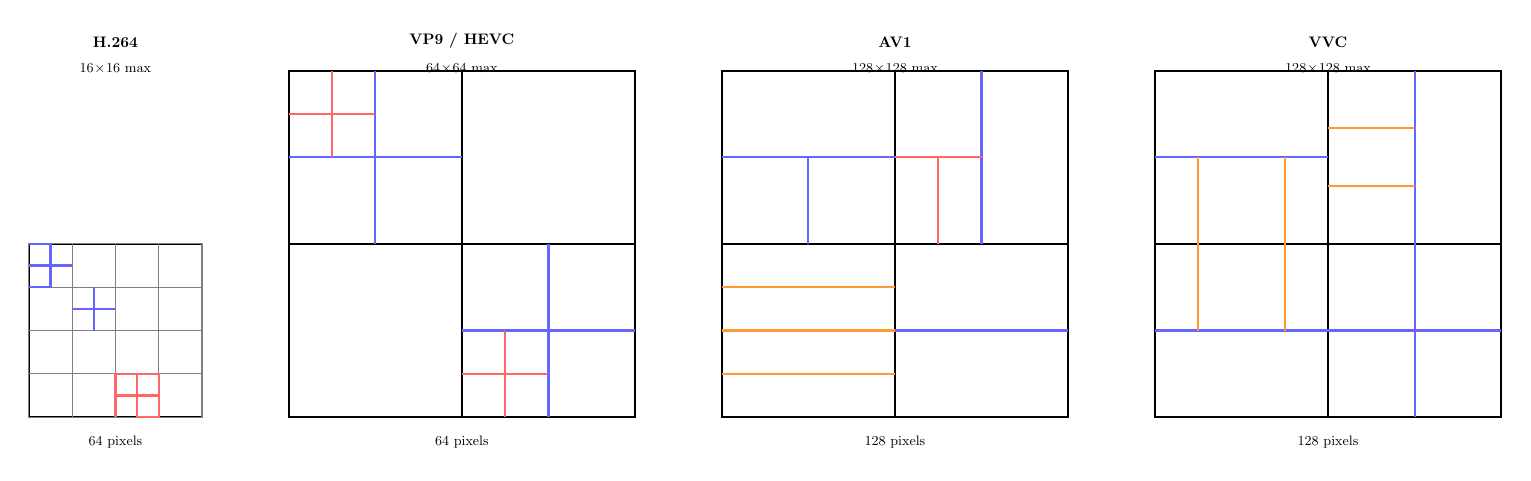
\begin{tikzpicture}[>=Stealth, scale=0.55, every node/.style={scale=0.55}]

% --- H.264 panel ---
\begin{scope}[xshift=0cm]
  \node[font=\normalsize\bfseries, anchor=south] at (2, 8.4) {H.264};
  \node[font=\small, anchor=south] at (2, 7.8) {$16\!\times\!16$ max};
  % 4x4 grid of 16x16 macroblocks in a 64x64 region
  \draw[thick] (0,0) rectangle (4,4);
  \draw[thick] (0,0) rectangle (4,4);
  % macroblock grid
  \foreach \x in {0,1,2,3} {
    \foreach \y in {0,1,2,3} {
      \draw[gray] (\x, \y) rectangle (\x+1, \y+1);
    }
  }
  % show some sub-partitions
  \draw[blue!60, thick] (0,3) -- (0.5,3) -- (0.5,4) -- (0,4);
  \draw[blue!60, thick] (0.5,3) -- (0.5,4);
  \draw[blue!60, thick] (0,3.5) -- (1,3.5);
  % 8x8 in another
  \draw[blue!60, thick] (1,2.5) -- (2,2.5);
  \draw[blue!60, thick] (1.5,2) -- (1.5,3);
  % 4x4 in another
  \draw[red!60, thick] (2,0) -- (2,1) -- (3,1) -- (3,0);
  \draw[red!60, thick] (2.5,0) -- (2.5,0.5);
  \draw[red!60, thick] (2,0.5) -- (2.5,0.5);
  \draw[red!60, thick] (2.5,0.5) -- (2.5,1);
  \draw[red!60, thick] (2.5,0) -- (3,0) -- (3,0.5) -- (2.5,0.5);
  % Scale label
  \node[font=\small, anchor=north] at (2, -0.3) {64 pixels};
\end{scope}

% --- VP9/HEVC panel ---
\begin{scope}[xshift=6cm]
  \node[font=\normalsize\bfseries, anchor=south] at (4, 8.4) {VP9 / HEVC};
  \node[font=\small, anchor=south] at (4, 7.8) {$64\!\times\!64$ max};
  % One 64x64 superblock
  \draw[thick] (0,0) rectangle (8,8);
  % quad-tree splits
  \draw[thick] (4,0) -- (4,8);
  \draw[thick] (0,4) -- (8,4);
  % further splits in top-left quadrant
  \draw[blue!60, thick] (2,4) -- (2,8);
  \draw[blue!60, thick] (0,6) -- (4,6);
  % further split in top-left-top-left
  \draw[red!60, thick] (1,6) -- (1,8);
  \draw[red!60, thick] (0,7) -- (2,7);
  % split bottom-right quadrant
  \draw[blue!60, thick] (6,0) -- (6,4);
  \draw[blue!60, thick] (4,2) -- (8,2);
  % deeper in bottom-right-bottom-left
  \draw[red!60, thick] (5,0) -- (5,2);
  \draw[red!60, thick] (4,1) -- (6,1);
  % Scale label
  \node[font=\small, anchor=north] at (4, -0.3) {64 pixels};
\end{scope}

% --- AV1 panel ---
\begin{scope}[xshift=16cm]
  \node[font=\normalsize\bfseries, anchor=south] at (4, 8.4) {AV1};
  \node[font=\small, anchor=south] at (4, 7.8) {$128\!\times\!128$ max};
  % 128x128 shown as 8x8 grid (each cell = 16px)
  \draw[thick] (0,0) rectangle (8,8);
  % quad split: top half / bottom half
  \draw[thick] (4,0) -- (4,8);
  \draw[thick] (0,4) -- (8,4);
  % rectangular splits in top-left
  \draw[blue!60, thick] (0,6) -- (4,6);
  \draw[blue!60, thick] (2,4) -- (2,6);
  % asymmetric in bottom-left (4:1 rect)
  \draw[orange!80, thick] (0,3) -- (4,3);
  \draw[orange!80, thick] (0,2) -- (4,2);
  \draw[orange!80, thick] (0,1) -- (4,1);
  % quad + rect in top-right
  \draw[blue!60, thick] (6,4) -- (6,8);
  \draw[red!60, thick] (4,6) -- (6,6);
  \draw[red!60, thick] (5,4) -- (5,6);
  % bottom-right: large blocks
  \draw[blue!60, thick] (4,2) -- (8,2);
  % Scale label
  \node[font=\small, anchor=north] at (4, -0.3) {128 pixels};
\end{scope}

% --- VVC panel ---
\begin{scope}[xshift=26cm]
  \node[font=\normalsize\bfseries, anchor=south] at (4, 8.4) {VVC};
  \node[font=\small, anchor=south] at (4, 7.8) {$128\!\times\!128$ max};
  \draw[thick] (0,0) rectangle (8,8);
  % quad split
  \draw[thick] (4,0) -- (4,8);
  \draw[thick] (0,4) -- (8,4);
  % binary split (horizontal) in top-left
  \draw[blue!60, thick] (0,6) -- (4,6);
  % ternary split (vertical) in top-left-bottom
  \draw[orange!80, thick] (1,4) -- (1,6);
  \draw[orange!80, thick] (3,4) -- (3,6);
  % binary split (vertical) in top-right
  \draw[blue!60, thick] (6,4) -- (6,8);
  % ternary horizontal in top-right-left
  \draw[orange!80, thick] (4,5.33) -- (6,5.33);
  \draw[orange!80, thick] (4,6.67) -- (6,6.67);
  % bottom-left: binary horizontal
  \draw[blue!60, thick] (0,2) -- (4,2);
  % deeper ternary in bottom-left-top
  \draw[orange!80, thick] (1,2) -- (1,4);
  \draw[orange!80, thick] (3,2) -- (3,4);
  % bottom-right: mostly large
  \draw[blue!60, thick] (6,0) -- (6,4);
  \draw[blue!60, thick] (4,2) -- (8,2);
  % Scale label
  \node[font=\small, anchor=north] at (4, -0.3) {128 pixels};
\end{scope}

\end{tikzpicture}
\caption{Block partitioning comparison across codec generations. H.264 is
  limited to $16\!\times\!16$ macroblocks with fixed sub-partitions (left).
  VP9/HEVC use quad-tree partitioning within $64\!\times\!64$ superblocks
  (center-left). AV1 extends to $128\!\times\!128$ with quad-tree plus
  rectangular splits (center-right). VVC adds binary and ternary splits for
  maximum flexibility (right). Blue lines show first-level splits; red
  shows deeper partitioning; orange shows asymmetric/ternary splits.}
\label{fig:block-partitioning}
\end{figure}

\begin{table}[ht]
\centering
\small
\renewcommand{\arraystretch}{1.4}
\begin{tabularx}{\textwidth}{lXXXXX}
\toprule
\textbf{Feature} & \textbf{H.264} & \textbf{VP9} & \textbf{HEVC}
  & \textbf{AV1} & \textbf{VVC} \\
\midrule
Max block &
  $16\!\times\!16$ &
  $64\!\times\!64$ &
  $64\!\times\!64$ &
  $128\!\times\!128$ &
  $128\!\times\!128$ \\
Min block &
  $4\!\times\!4$ &
  $4\!\times\!4$ &
  $8\!\times\!8$ &
  $4\!\times\!4$ &
  $4\!\times\!4$ \\
Split types &
  Fixed partitions &
  Quad-tree &
  Quad-tree &
  Quad $+$ rect &
  Quad $+$ BT $+$ TT \\
Asymmetric &
  Limited &
  No &
  No &
  4:1 rectangles &
  Full (BT/TT) \\
\bottomrule
\end{tabularx}
\caption{Block partitioning capabilities by codec. BT = binary tree
  (horizontal or vertical), TT = ternary tree (1:2:1 split). Larger maximum
  blocks reduce overhead for homogeneous regions; asymmetric splits improve
  partitioning efficiency at content boundaries.}
\label{tab:partitioning}
\end{table}

%% ---------------------------------------------------------------------------
\subsection{Rate-Distortion Operating Points by Codec}
\label{sec:rd-comparison}

The codec-specific analyses of
Sections~\ref{sec:mpeg-lineage}--\ref{sec:aom-lineage} can be unified
through the Bj\o ntegaard Delta Rate (BD-Rate), the standard metric for
comparing codec efficiency. BD-Rate computes the average percentage rate
difference between two codecs at equivalent distortion by integrating the
difference between their rate-distortion curves fit as cubic polynomials in
PSNR-vs-log-rate space:
\begin{equation}
  \text{BD-Rate} = \frac{1}{\Delta\text{PSNR}}
    \int_{\text{PSNR}_{\min}}^{\text{PSNR}_{\max}}
    \left[ \ln R_A(p) - \ln R_B(p) \right] dp
  \label{eq:bd-rate}
\end{equation}
A negative BD-Rate indicates that codec~$A$ requires fewer bits than
codec~$B$ at the same quality.

\begin{figure}[ht]
\centering
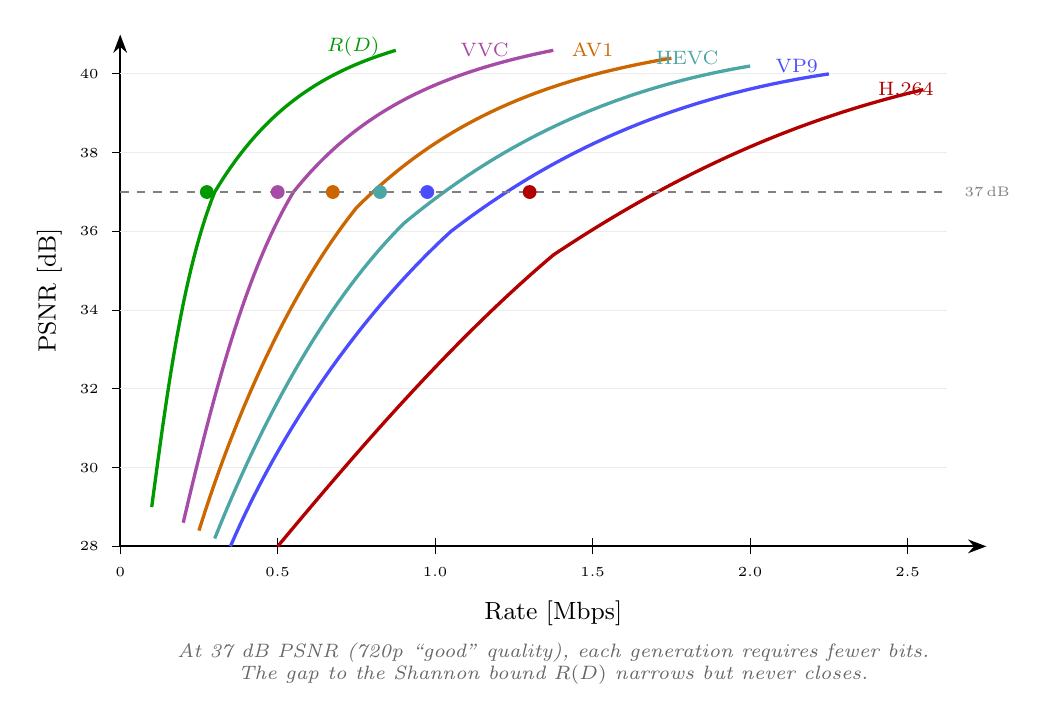
\begin{tikzpicture}[>=Stealth]

% --- Axes ---
\draw[->, thick] (0, 0) -- (11, 0);
\draw[->, thick] (0, 0) -- (0, 6.5);

% --- Axis titles ---
\node[font=\small] at (5.5, -0.85) {Rate [Mbps]};
\node[font=\small, rotate=90] at (-0.9, 3.25) {PSNR [dB]};

% --- X-axis labels ---
\foreach \x/\lab in {0/0, 2/0.5, 4/1.0, 6/1.5, 8/2.0, 10/2.5} {
  \draw (\x, -0.1) -- (\x, 0.1);
  \node[font=\tiny, anchor=north] at (\x, -0.15) {\lab};
}

% --- Y-axis labels ---
\foreach \y/\lab in {0/28, 1/30, 2/32, 3/34, 4/36, 5/38, 6/40} {
  \draw (-0.1, \y) -- (0.1, \y);
  \node[font=\tiny, anchor=east] at (-0.15, \y) {\lab};
}

% --- Grid ---
\foreach \y in {1,2,3,4,5,6} {
  \draw[gray!15] (0, \y) -- (10.5, \y);
}

% --- Shannon R(D) bound (leftmost curve) ---
\draw[very thick, green!60!black]
  (0.4, 0.5) .. controls (0.6, 2) and (0.8, 3.5) ..
  (1.2, 4.5) .. controls (1.8, 5.5) and (2.5, 6.0) ..
  (3.5, 6.3);
\node[font=\scriptsize, green!60!black, anchor=south west] at (2.5, 6.1)
  {$R(D)$};

% --- VVC curve ---
\draw[very thick, violet!70]
  (0.8, 0.3) .. controls (1.2, 2.0) and (1.6, 3.5) ..
  (2.2, 4.5) .. controls (3.0, 5.5) and (4.0, 6.0) ..
  (5.5, 6.3);
\node[font=\scriptsize, violet!70, anchor=south west] at (4.2, 6.1)
  {VVC};

% --- AV1 curve ---
\draw[very thick, orange!80!black]
  (1.0, 0.2) .. controls (1.5, 1.8) and (2.2, 3.3) ..
  (3.0, 4.3) .. controls (4.0, 5.3) and (5.2, 5.9) ..
  (7.0, 6.2);
\node[font=\scriptsize, orange!80!black, anchor=south] at (6.0, 6.1)
  {AV1};

% --- HEVC curve ---
\draw[very thick, teal!70]
  (1.2, 0.1) .. controls (1.8, 1.6) and (2.6, 3.1) ..
  (3.6, 4.1) .. controls (4.8, 5.1) and (6.2, 5.8) ..
  (8.0, 6.1);
\node[font=\scriptsize, teal!70, anchor=south] at (7.2, 6.0)
  {HEVC};

% --- VP9 curve ---
\draw[very thick, blue!70]
  (1.4, 0.0) .. controls (2.0, 1.4) and (3.0, 2.9) ..
  (4.2, 4.0) .. controls (5.5, 5.0) and (7.0, 5.7) ..
  (9.0, 6.0);
\node[font=\scriptsize, blue!70, anchor=south west] at (8.2, 5.9)
  {VP9};

% --- H.264 curve (rightmost) ---
\draw[very thick, red!70!black]
  (2.0, 0.0) .. controls (3.0, 1.2) and (4.2, 2.6) ..
  (5.5, 3.7) .. controls (7.0, 4.7) and (8.5, 5.4) ..
  (10.2, 5.8);
\node[font=\scriptsize, red!70!black, anchor=south west] at (9.5, 5.6)
  {H.264};

% --- 37 dB reference line ---
\draw[thin, gray, dashed] (0, 4.5) -- (10.5, 4.5);
\node[font=\tiny, gray, anchor=west] at (10.6, 4.5) {37\,dB};

% --- Operating points at 37 dB ---
\fill[red!70!black] (5.2, 4.5) circle (2.5pt);
\fill[blue!70] (3.9, 4.5) circle (2.5pt);
\fill[teal!70] (3.3, 4.5) circle (2.5pt);
\fill[orange!80!black] (2.7, 4.5) circle (2.5pt);
\fill[violet!70] (2.0, 4.5) circle (2.5pt);
\fill[green!60!black] (1.1, 4.5) circle (2.5pt);

% --- Annotation ---
\node[font=\scriptsize\itshape, text=black!60, align=center,
  anchor=north] at (5.5, -1.1)
  {At 37~dB PSNR (720p ``good'' quality), each generation
  requires fewer bits.\\
  The gap to the Shannon bound $R(D)$ narrows but never closes.};

\end{tikzpicture}
\caption{Rate-distortion curves for six codecs at 720p/30fps, with the
  Shannon $R(D)$ bound (green). At constant quality (37~dB dashed line),
  the rate progression from H.264 through VVC illustrates the BD-Rate
  savings in Table~\ref{tab:bd-rate}. This figure extends
  Figure~\ref{fig:rate-distortion} from Appendix~\ref{app:info-theory}
  with the full codec lineage.}
\label{fig:rd-curves-detailed}
\end{figure}

\begin{table}[ht]
\centering
\small
\renewcommand{\arraystretch}{1.4}
\begin{tabularx}{\textwidth}{lXXXX}
\toprule
\textbf{Codec} & \textbf{BD-Rate vs.\ H.264}
  & \textbf{$\Delta$ (720p)} & \textbf{Family} & \textbf{Year} \\
\midrule
VP8  & ${\sim}$0\%    & ${\sim}$2.1 & Google    & 2010 \\
VP9  & $-$35\%        & ${\sim}$0.8 & AOM       & 2013 \\
HEVC & $-$40\%        & ${\sim}$0.7 & MPEG/ITU  & 2013 \\
AV1  & $-$54\%        & ${\sim}$0.5 & AOM       & 2018 \\
VVC  & $-$63\%        & ${\sim}$0.3 & MPEG/ITU  & 2020 \\
\bottomrule
\end{tabularx}
\caption{BD-Rate savings and coding efficiency gap $\Delta$
  (eq.~\ref{eq:coding-gap}) for each codec relative to H.264 at 720p/30fps.
  The two families (MPEG/ITU and Google/AOM) achieve comparable efficiency
  within each generation; AV1 slightly trails HEVC, VVC leads AV1 by
  ${\sim}$20\%.}
\label{tab:bd-rate}
\end{table}

Table~\ref{tab:bd-rate} provides the DSP-grounded explanation for the codec
ordering in eq.~(\ref{eq:codec-ordering}) and the savings figures in
eqs.~(\ref{eq:vp9-savings})--(\ref{eq:av1-savings}): each generation adds
tools that reduce $\Delta_{\text{pred}}$, $\Delta_{\text{transform}}$, and
$\Delta_{\text{quant}}$ in (\ref{eq:delta-decomp}), with diminishing
returns as the Shannon bound is approached.

%% ---------------------------------------------------------------------------
\subsection{Scalable Video Coding and Simulcast}
\label{sec:svc-simulcast}

Multi-participant WebRTC sessions require adaptive quality: different
receivers have different bandwidths, and a single encode rate cannot serve
all. Two architectures address this.

\subsubsection{Simulcast}
\label{sec:simulcast}

Simulcast encodes the source at $N$ independent resolution/bitrate
combinations:
\begin{equation}
  R_{\text{simulcast}} = \sum_{i=1}^{N} R_i
  \label{eq:simulcast-rate}
\end{equation}
Each encoding is a fully independent bitstream. A Selective Forwarding
Unit (SFU) selects which stream to forward to each receiver based on
reported bandwidth. The overhead is substantial: a typical 3-layer
simulcast (720p/1.5~Mbps, 360p/500~kbps, 180p/150~kbps) requires
2.15~Mbps total---approximately 1.4$\times$ the cost of the highest
layer alone---with no inter-layer compression benefit.

\subsubsection{Scalable Video Coding (SVC)}
\label{sec:svc}

SVC produces a layered bitstream where a base layer $L_0$ is independently
decodable and enhancement layers $L_1, \ldots, L_K$ refine quality
progressively. Three scalability dimensions exist:

\textbf{Temporal scalability.} The base layer encodes at a reduced frame
rate (e.g., 7.5~fps); enhancement layers add intermediate frames:
\begin{equation}
  R_{\text{temporal}} = R_0 + \sum_{k=1}^{K} \Delta R_k
  \label{eq:temporal-svc}
\end{equation}
where $\Delta R_k \ll R_0$ because enhancement frames reference lower
layers and carry primarily motion-compensated residuals. An SFU drops
enhancement layers for bandwidth-constrained receivers, gracefully
degrading frame rate while preserving spatial quality.

\textbf{Spatial scalability.} The base layer encodes at reduced resolution;
enhancement layers add detail via inter-layer prediction:
\begin{equation}
  R_{\text{spatial}} = R_0 + \Delta R_{\text{upscale}}
  \label{eq:spatial-svc}
\end{equation}
where $\Delta R_{\text{upscale}}$ exploits correlation between the
upsampled base layer and the full-resolution source.

\textbf{Quality (SNR) scalability.} Refinement of quantization at the same
resolution, encoded as the difference between coarse and fine
reconstructions.

SVC achieves 20--30\% rate savings over simulcast for equivalent
adaptivity because enhancement layers exploit inter-layer prediction:
\begin{equation}
  R_{\text{SVC}} < R_{\text{simulcast}} \quad
  \text{(typically by 20--30\%)}
  \label{eq:svc-advantage}
\end{equation}

\begin{figure}[ht]
\centering
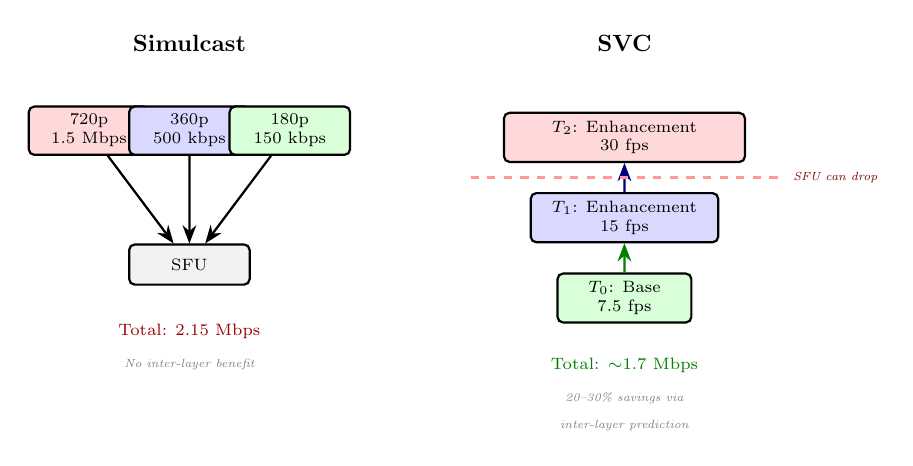
\begin{tikzpicture}[>=Stealth, scale=0.85, every node/.style={scale=0.85},
  layer/.style={draw, rounded corners=2pt, minimum width=1.8cm,
    minimum height=0.6cm, font=\scriptsize, align=center, thick}]

% --- Simulcast (left) ---
\node[font=\normalsize\bfseries] at (2, 5.8) {Simulcast};

% Three independent columns
\node[layer, fill=red!15] (s720) at (0.5, 4.5) {720p\\1.5 Mbps};
\node[layer, fill=blue!15] (s360) at (2.0, 4.5) {360p\\500 kbps};
\node[layer, fill=green!15] (s180) at (3.5, 4.5) {180p\\150 kbps};

\node[layer, fill=gray!10] (sfu1) at (2.0, 2.5) {SFU};

\draw[->, thick] (s720) -- (sfu1);
\draw[->, thick] (s360) -- (sfu1);
\draw[->, thick] (s180) -- (sfu1);

\node[font=\scriptsize, text=red!60!black] at (2.0, 1.5)
  {Total: 2.15 Mbps};
\node[font=\tiny\itshape, text=black!50] at (2.0, 1.0)
  {No inter-layer benefit};

% --- SVC (right) ---
\node[font=\normalsize\bfseries] at (8.5, 5.8) {SVC};

% Pyramid
\node[layer, fill=green!15, minimum width=2.0cm] (t0) at (8.5, 2.0)
  {$T_0$: Base\\7.5 fps};
\node[layer, fill=blue!15, minimum width=2.8cm] (t1) at (8.5, 3.2)
  {$T_1$: Enhancement\\15 fps};
\node[layer, fill=red!15, minimum width=3.6cm] (t2) at (8.5, 4.4)
  {$T_2$: Enhancement\\30 fps};

% Dependency arrows
\draw[->, thick, green!50!black] (t0) -- (t1);
\draw[->, thick, blue!50!black] (t1) -- (t2);

% Drop annotations
\draw[thick, dashed, red!40] (6.2, 3.8) -- (10.8, 3.8);
\node[font=\tiny\itshape, text=red!50!black, anchor=west] at (10.9, 3.8)
  {SFU can drop};

\node[font=\scriptsize, text=green!50!black] at (8.5, 1.0)
  {Total: ${\sim}$1.7 Mbps};
\node[font=\tiny\itshape, text=black!50] at (8.5, 0.5)
  {20--30\% savings via};
\node[font=\tiny\itshape, text=black!50] at (8.5, 0.1)
  {inter-layer prediction};

\end{tikzpicture}
\caption{Simulcast (left) encodes three independent bitstreams with no
  inter-layer compression. SVC (right) encodes a layered bitstream where
  temporal enhancement layers ($T_1$, $T_2$) reference the base layer
  ($T_0$), achieving 20--30\% savings. The SFU drops enhancement layers
  for bandwidth-constrained receivers.}
\label{fig:svc-architecture}
\end{figure}

Codec-specific SVC support relevant to WebRTC:

\begin{itemize}
\item \textbf{H.264 SVC (Annex~G).} Defines temporal, spatial, and quality
  scalability. Complex to implement; rarely used in WebRTC deployments.

\item \textbf{VP9 SVC.} Temporal scalability is widely deployed in WebRTC
  via libvpx (up to 3~temporal layers). Spatial SVC is defined but
  implementation-limited. VP9 temporal SVC is the primary mechanism
  enabling adaptive quality in Chrome/Firefox SFU-based calls.

\item \textbf{AV1 SVC.} Temporal scalability supported in both libaom and
  SVT-AV1. A key enabler for AV1 adoption in production WebRTC
  infrastructure, as SFUs require layered bitstreams to serve heterogeneous
  receivers.
\end{itemize}

Safari's lack of simulcast and SVC support in 2021 (Section~3.1) meant
that Safari users in multi-participant calls could not benefit from adaptive
quality---every receiver got the same stream regardless of bandwidth,
degrading the experience for all participants.

%% ---------------------------------------------------------------------------
\subsection{Hardware vs.\ Software Encoding}
\label{sec:hw-sw}

The main paper identifies hardware encoding as the deployment gate for
AV1 (Sections~8.5, 9.5). This section quantifies why.

\subsubsection{Encoding Complexity}

The computational cost of encoding a video frame is dominated by motion
estimation and RD-optimized mode decision. We express complexity as
operations per pixel:
\begin{equation}
  C_{\text{enc}} = C_{\text{ME}} + C_{\text{transform}}
    + C_{\text{quant}} + C_{\text{entropy}}
    + C_{\text{mode}}
  \label{eq:enc-complexity}
\end{equation}

Representative values for real-time presets:

\begin{itemize}
\item H.264 Constrained Baseline (``veryfast''): $C_{\text{enc}} \approx
  200$~ops/pixel
\item VP9 (speed~8, real-time): $C_{\text{enc}} \approx 600$~ops/pixel
\item AV1 (speed~10, real-time): $C_{\text{enc}} \approx 2000$~ops/pixel
\end{itemize}

The real-time constraint requires:
\begin{equation}
  C_{\text{enc}} \times W \times H \times \text{fps}
    \leq F_{\text{available}}
  \label{eq:realtime-constraint}
\end{equation}
where $F_{\text{available}}$ is the available computational throughput
(operations per second). For 720p/30fps AV1 at 2000~ops/pixel:
\begin{equation}
  2000 \times 921{,}600 \times 30 = 55.3 \times 10^9 \;\text{ops/s}
  \label{eq:av1-cost}
\end{equation}
This consumes approximately one full core of a modern desktop CPU. On
mobile devices with thermal and power constraints, software AV1 encoding
at 720p/30fps remains impractical without hardware acceleration.

\subsubsection{Hardware Encoder Architecture}

Hardware encoders implement a fixed subset of the codec's tool set in
dedicated silicon. The trade-off is quality for throughput: hardware
encoders typically produce output 10--20\% larger than software encoders
at equivalent visual quality because they implement fewer mode decision
candidates and simpler motion search:
\begin{equation}
  \Delta_{\text{HW}} \approx (1.1 \text{--} 1.2)
    \cdot \Delta_{\text{SW}}
  \label{eq:hw-quality-gap}
\end{equation}

This quality penalty is acceptable for real-time communication because:
(a)~the alternative---software encoding at a lower speed preset or reduced
resolution---incurs a larger quality penalty, and (b)~the freed CPU
capacity can be used for pre/post-processing, noise reduction, or
additional application logic.

\subsubsection{Hardware Encoder Availability}

\begin{table}[ht]
\centering
\small
\renewcommand{\arraystretch}{1.4}
\begin{tabularx}{\textwidth}{lXXXX}
\toprule
\textbf{Platform} & \textbf{H.264 HW} & \textbf{VP9 HW encode}
  & \textbf{AV1 HW encode} & \textbf{AV1 year} \\
\midrule
Intel (QSV) &
  Sandy Bridge+ (2011) &
  Kaby Lake+ (2017) &
  Arc / Meteor Lake+ &
  2022 \\
NVIDIA (NVENC) &
  Kepler+ (2012) &
  --- &
  Ada Lovelace+ &
  2022 \\
AMD (VCN) &
  VCN~1.0+ (2017) &
  --- &
  VCN~4.0+ (RDNA~3) &
  2023 \\
Apple (VideoToolbox) &
  A4+ (2010) &
  --- &
  M3+ &
  2023 \\
Qualcomm &
  SD~820+ (2016) &
  --- &
  SD~8 Gen~2+ &
  2023 \\
\bottomrule
\end{tabularx}
\caption{Hardware encoder availability timeline. H.264 hardware encoding
  has been ubiquitous for over a decade. AV1 hardware encoding began
  shipping in 2022--2023 across all major platforms; the main paper projects
  it becomes the practical WebRTC default by 2028--2030 as these chipsets
  reach market saturation.}
\label{tab:hw-encoders}
\end{table}

\excursus{Excursus: WebCodecs and hardware acceleration.}{When a WebCodecs
\texttt{VideoEncoder} is configured with \texttt{codec: "av01"}, the browser
selects hardware or software encoding based on platform capability and the
\texttt{hardwareAcceleration} preference (\texttt{"prefer-hardware"},
\texttt{"prefer-software"}, or \texttt{"no-preference"}). The application
receives encoded \texttt{EncodedVideoChunk} objects either way, but latency
and CPU cost differ dramatically: hardware encoding typically adds
$<\!1$~ms per frame and consumes near-zero CPU, while software AV1 at
real-time presets consumes an entire CPU core
(eq.~\ref{eq:av1-cost}). This abstraction is what makes the hardware
timeline in Table~\ref{tab:hw-encoders} directly relevant to the WebCodecs
adoption curve in Section~7.}

The hardware encoding timeline directly underpins the main paper's
projections: the ``AV1 becomes practical'' milestone (Section~8.5) and
``AV1 HW ubiquitous'' milestone (Section~9.5) depend on the chipset
generations in Table~\ref{tab:hw-encoders} reaching market saturation.

%% ---------------------------------------------------------------------------
\subsection{Implications for Real-Time Web Communication}
\label{sec:video-implications}

The DSP analysis of this appendix maps back to concrete implications for
the technologies surveyed in the main text.

\textbf{The hybrid coding framework is universal; innovation is
incremental.} Every codec from VP8 to VVC implements the same
prediction--transform--quantization--entropy framework
(Figure~\ref{fig:hybrid-encoder}). Generational improvements come from
expanding the tool set within this framework---more block sizes
(Table~\ref{tab:partitioning}), more prediction modes, more transform
types (Table~\ref{tab:transforms})---not from fundamentally new
architectures. This means the efficiency gap $\Delta$ approaches but never
reaches zero: each additional tool yields diminishing rate-distortion
improvement at increasing computational cost.

\textbf{Transform and prediction innovations explain the BD-Rate
progression.} The 35\% rate saving from H.264 to VP9 comes primarily from
larger blocks ($64\!\times\!64$ vs.\ $16\!\times\!16$) and adaptive
transforms (DCT$+$ADST vs.\ fixed DCT). The additional 30\% from VP9 to
AV1 comes from compound and warped motion, film grain synthesis, and
16-way transform type selection (Table~\ref{tab:bd-rate}). Each tool adds
encoding complexity proportional to its rate-distortion benefit, which is
why real-time encoders must aggressively prune the tool set.

\textbf{SVC is what makes multi-participant WebRTC work.} Without temporal
SVC, an SFU must forward full-rate streams to all participants regardless
of their bandwidth. With VP9/AV1 temporal SVC
(Section~\ref{sec:svc}), the SFU drops enhancement temporal layers for
bandwidth-constrained receivers, degrading frame rate gracefully while
preserving spatial quality. The 20--30\% savings over simulcast
(eq.~\ref{eq:svc-advantage}) translate directly to reduced server egress
bandwidth in large meetings.

\textbf{Hardware encoding is the deployment gate, not codec specification.}
AV1 was specified in 2018 but becomes a practical WebRTC default only
when hardware encoders are ubiquitous (${\sim}$2028--2030). The DSP tools
that make AV1 efficient---warped motion, OBMC, $128\!\times\!128$
superblocks with flexible partitioning---are precisely the tools that make
it computationally expensive in software (eq.~\ref{eq:av1-cost}). The
${\sim}$10--20\% quality penalty of hardware encoders
(eq.~\ref{eq:hw-quality-gap}) is the price of real-time feasibility, and
it is a price worth paying: $\Delta_{\text{AV1,HW}} \approx 0.6$ is still
far below $\Delta_{\text{VP9,SW}} \approx 0.8$.

\textbf{The convergence toward Shannon is real but asymptotic.}
Cross-referencing with Appendix~\ref{app:info-theory}: H.264's
$\Delta \approx 2.1$ means it operates at $3.1\times$ the theoretical
minimum rate. VP9's $\Delta \approx 0.8$ means $1.8\times$. AV1's
$\Delta \approx 0.5$ means $1.5\times$. VVC's $\Delta \approx 0.3$ means
$1.3\times$. Each generation captures more spatial, temporal, and
perceptual redundancy, but the returns are diminishing: the distance from
H.264 to VP9 ($-$35\%) exceeds VP9 to AV1 ($-$30\%), which exceeds AV1 to
VVC ($-$17\%). The next generation of efficiency gains for real-time web
communication will come not from codecs alone, but from the co-optimization
of transport (QUIC, WebTransport), application architecture (WebCodecs,
unbundled pipelines), and network infrastructure that the main text
describes.

%
% Requires in the preamble: amsmath, amssymb, tabularx, booktabs

\section{Video Compression Fundamentals}
\label{app:video-compression}

Appendix~\ref{app:info-theory} quantified the coding efficiency gap $\Delta$
(eq.~\ref{eq:coding-gap}) for each codec generation, treating codecs as black
boxes characterized by their distance from the Shannon rate-distortion bound.
This appendix opens those black boxes. We examine the signal processing and
coding techniques that determine $\Delta$: how video codecs exploit spatial,
temporal, and perceptual redundancy, what distinguishes one codec generation
from the next, and why computational complexity---not algorithmic
capability---remains the binding constraint for real-time web communication.

%% ---------------------------------------------------------------------------
\subsection{Why Video Is Compressible}
\label{sec:compressible}

A raw digital video signal carries far more data than information. Three
fundamental redundancies make compression ratios of 200:1 to 500:1 achievable
at perceptually acceptable quality.

\subsubsection{Spatial Redundancy}

Natural images exhibit strong local correlation. The autocorrelation function
for a typical image row can be modeled as a first-order Markov process:
\begin{equation}
  R_{xx}(k) = \sigma^2 \rho^{|k|}
  \label{eq:spatial-autocorr}
\end{equation}
where $\sigma^2$ is the pixel variance and $\rho \in [0.90, 0.97]$ for
natural content. The separable two-dimensional extension is:
\begin{equation}
  R_{xx}(k, l) = \sigma^2 \,\rho_h^{|k|}\, \rho_v^{|l|}
  \label{eq:spatial-autocorr-2d}
\end{equation}
The power spectral density---the Fourier transform of
(\ref{eq:spatial-autocorr-2d})---is concentrated at low spatial frequencies,
meaning most of the signal energy occupies a small fraction of the frequency
domain. This concentration is the foundation of transform coding
(Section~\ref{sec:transforms}).

\subsubsection{Temporal Redundancy}

Consecutive video frames are highly correlated. For typical conversational
video at 30~fps, the inter-frame correlation coefficient is:
\begin{equation}
  \text{Corr}(f_t, f_{t-1}) \approx 0.90\text{--}0.98
  \label{eq:temporal-corr}
\end{equation}
Most pixels change little between frames; only regions containing motion,
lighting changes, or scene cuts carry significant new information. Motion
estimation (Section~\ref{sec:motion}) exploits this by predicting each block
from a displaced version of a reference frame, transmitting only the
prediction residual.

\subsubsection{Perceptual Irrelevance}

The human visual system (HVS) has lower spatial acuity for chrominance than
luminance. This asymmetry motivates \emph{chroma subsampling}: representing
color difference channels at reduced resolution relative to the luma channel.

\excursus{Excursus: Why 4:2:0?}{All WebRTC codecs operate on YCbCr 4:2:0
video, where each chroma channel is sampled at half the horizontal and half
the vertical resolution of luma. This reduces the sample count by a factor of
$1 + 0.25 + 0.25 = 1.5$ relative to $1 + 1 + 1 = 3$ for full-resolution
4:4:4 color, a 2$\times$ saving before any coding begins. Perceptual
experiments confirm that 4:2:0 is essentially indistinguishable from 4:4:4 at
typical viewing distances for video conferencing---the HVS cannot resolve
the missing chroma detail.}

\subsubsection{The Compression Imperative}

A raw 720p/30fps 4:2:0 video stream at 8~bits per sample requires:
\begin{equation}
  R_{\text{raw}} = 1280 \times 720 \times 1.5 \times 8 \times 30
    = 331.8 \;\text{Mbps}
  \label{eq:raw-rate}
\end{equation}
This exceeds the 120~Mbps median link capacity cited in
Table~\ref{tab:inet}. The Shannon rate-distortion bound
(eq.~\ref{eq:rate-distortion}) yields approximately 0.7--1.5~Mbps at
perceptually acceptable distortion---a compression ratio of 220:1 to 475:1.
Video compression is not optional for real-time communication; it is a
prerequisite.

The first-order entropy of raw pixel values $H(X)$ greatly exceeds the
conditional entropy given neighboring samples:
\begin{equation}
  H(X) \gg H(X \mid X_{\text{neighbors}})
  \label{eq:conditional-entropy}
\end{equation}
This gap---the mutual information between a pixel and its
neighbors---represents the exploitable redundancy. The entire hybrid coding
framework (Section~\ref{sec:hybrid}) is designed to extract this mutual
information through prediction, leaving only the irreducible residual for
transform coding and quantization.

%% ---------------------------------------------------------------------------
\subsection{The Hybrid Coding Framework}
\label{sec:hybrid}

Every major video codec since H.261 (1988)---including every codec in the
WebRTC stack---is a variation on the \emph{block-based hybrid coding}
framework. The encoder partitions each frame into blocks, predicts each block
from previously coded data, transforms and quantizes the prediction residual,
and entropy codes the result.

\subsubsection{Encoder Signal Flow}

For a block at position $(x,y)$ in frame $f_t$, the encoder computes a
prediction $\hat{f}_{\text{pred}}(x,y)$ from either the current frame
(intra prediction) or a reference frame (inter prediction). The prediction
residual is:
\begin{equation}
  e(x,y) = f_t(x,y) - \hat{f}_{\text{pred}}(x,y)
  \label{eq:residual}
\end{equation}
The residual is transformed, quantized, and entropy coded to produce the
bitstream. The decoder reconstructs the frame as:
\begin{equation}
  \hat{f}(x,y) = \hat{e}(x,y) + \hat{f}_{\text{pred}}(x,y)
  \label{eq:reconstruction}
\end{equation}
where $\hat{e}$ is the inverse-transformed, dequantized residual.

\subsubsection{Rate-Distortion Optimization}

Every coding decision---block partition, prediction mode, motion vector,
transform type, quantization level---is made by minimizing a Lagrangian
rate-distortion cost:
\begin{equation}
  J(m) = D(m) + \lambda \cdot R(m)
  \label{eq:rd-cost}
\end{equation}
where $m \in \mathcal{M}$ is a coding mode, $D(m)$ is the distortion
(typically sum of squared errors), $R(m)$ is the bit cost, and $\lambda$ is a
Lagrange multiplier controlling the rate-distortion trade-off. The optimal
mode satisfies:
\begin{equation}
  m^* = \arg\min_{m \in \mathcal{M}} \left[ D(m) + \lambda \cdot R(m) \right]
  \label{eq:rd-opt}
\end{equation}
The Lagrange multiplier relates to the quantization parameter (QP) via an
empirically validated exponential relationship:
\begin{equation}
  \lambda = c \cdot 2^{(QP - 12)/3}
  \label{eq:lambda-qp}
\end{equation}
where $c$ is a codec-specific constant. This relationship ensures that
finer quantization (lower QP) assigns higher cost to bits, favoring modes
that reduce distortion, while coarser quantization (higher QP) favors
modes that reduce rate.

\begin{figure}[ht]
\centering
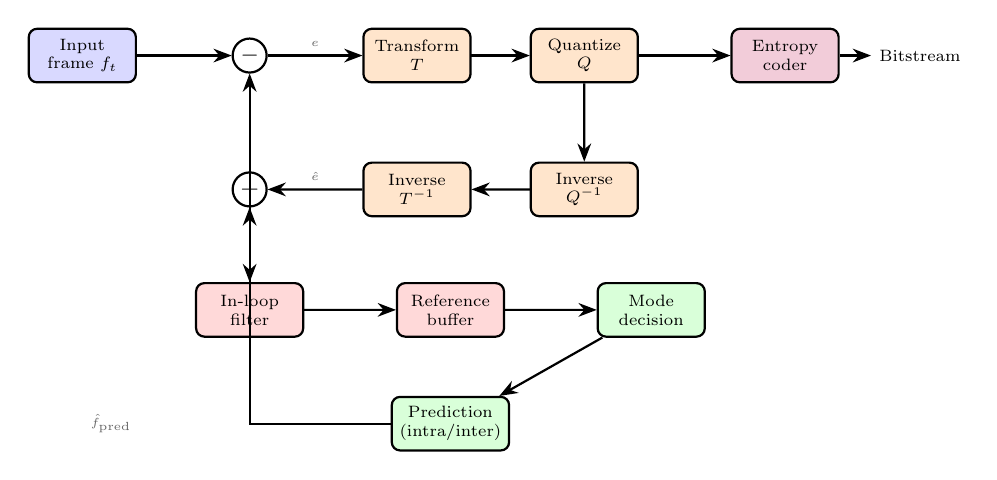
\begin{tikzpicture}[>=Stealth, scale=0.85, every node/.style={scale=0.85},
  block/.style={draw, rounded corners=3pt, minimum width=1.6cm,
    minimum height=0.8cm, font=\scriptsize, align=center, thick},
  arrow/.style={->, thick},
  label/.style={font=\tiny, text=black!60}]

% --- Input ---
\node[block, fill=blue!15] (input) at (0, 0) {Input\\frame $f_t$};

% --- Subtract ---
\node[draw, circle, inner sep=1.5pt, thick] (sub) at (2.5, 0) {$-$};

% --- Transform ---
\node[block, fill=orange!20] (transform) at (5, 0) {Transform\\$T$};

% --- Quantize ---
\node[block, fill=orange!20] (quant) at (7.5, 0) {Quantize\\$Q$};

% --- Entropy ---
\node[block, fill=purple!20] (entropy) at (10.5, 0) {Entropy\\coder};

% --- Bitstream ---
\node[font=\scriptsize, right=0.4cm of entropy] (bitstream) {Bitstream};

% --- Inverse Quantize ---
\node[block, fill=orange!20] (iquant) at (7.5, -2) {Inverse\\$Q^{-1}$};

% --- Inverse Transform ---
\node[block, fill=orange!20] (itransform) at (5, -2) {Inverse\\$T^{-1}$};

% --- Add ---
\node[draw, circle, inner sep=1.5pt, thick] (add) at (2.5, -2) {$+$};

% --- In-loop filter ---
\node[block, fill=red!15] (filter) at (2.5, -3.8) {In-loop\\filter};

% --- Reference buffer ---
\node[block, fill=red!15] (refbuf) at (5.5, -3.8) {Reference\\buffer};

% --- Mode decision ---
\node[block, fill=green!15] (mode) at (8.5, -3.8) {Mode\\decision};

% --- Prediction ---
\node[block, fill=green!15] (pred) at (5.5, -5.5) {Prediction\\(intra/inter)};

% --- Forward path ---
\draw[arrow] (input) -- (sub);
\draw[arrow] (sub) -- node[above, label] {$e$} (transform);
\draw[arrow] (transform) -- (quant);
\draw[arrow] (quant) -- (entropy);
\draw[arrow] (entropy) -- (bitstream);

% --- Reconstruction path ---
\draw[arrow] (quant) -- (iquant);
\draw[arrow] (iquant) -- (itransform);
\draw[arrow] (itransform) -- node[above, label] {$\hat{e}$} (add);

% --- Filter and buffer ---
\draw[arrow] (add) -- (filter);
\draw[arrow] (filter) -- (refbuf);

% --- Prediction feedback ---
\draw[arrow] (refbuf) -- (mode);
\draw[arrow] (mode) -- (pred);
\draw[arrow] (pred) -| (sub);
\draw[arrow] (pred) -| (add);

% --- Labels ---
\node[label, anchor=west] at (0, -5.5) {$\hat{f}_{\text{pred}}$};

\end{tikzpicture}
\caption{Block-based hybrid encoder architecture. Every codec from H.264
  through VVC follows this structure: predict each block from previously
  coded data (green), transform and quantize the residual (orange), entropy
  code the result (purple), then reconstruct and filter for future
  reference (red). The coding efficiency gap $\Delta$
  (eq.~\ref{eq:coding-gap}) arises from sub-optimal prediction, imperfect
  energy compaction, quantization beyond the rate-distortion bound, and
  entropy coding overhead.}
\label{fig:hybrid-encoder}
\end{figure}

The four sub-optimal components of Figure~\ref{fig:hybrid-encoder}---prediction,
transform, quantization, and entropy coding---each contribute to $\Delta$:
\begin{equation}
  \Delta \approx \Delta_{\text{pred}} + \Delta_{\text{transform}}
    + \Delta_{\text{quant}} + \Delta_{\text{entropy}}
  \label{eq:delta-decomp}
\end{equation}
Generational codec improvements reduce one or more of these terms. The codec
lineages in Sections~\ref{sec:mpeg-lineage}--\ref{sec:aom-lineage} trace
exactly which tools target which terms.

%% ---------------------------------------------------------------------------
\subsection{Transforms}
\label{sec:transforms}

The transform stage decorrelates the prediction residual, concentrating
energy into a few coefficients that can be efficiently quantized and coded.

\subsubsection{The KLT and Its DCT Approximation}
\label{sec:klt-dct}

The optimal decorrelating transform for a stationary source is the
\emph{Karhunen-Lo\`eve Transform} (KLT), whose basis vectors are the
eigenvectors of the input autocorrelation matrix $\mathbf{R}_{xx}$. For a
first-order Markov source with correlation $\rho$ (eq.~\ref{eq:spatial-autocorr}),
the KLT basis converges to the Type-II DCT as block size grows:
\begin{equation}
  C_k(n) = \alpha_k \cos\!\left[\frac{\pi k (2n+1)}{2N}\right],
  \quad k,n = 0, \ldots, N-1
  \label{eq:dct-ii}
\end{equation}
where $\alpha_0 = \sqrt{1/N}$ and $\alpha_k = \sqrt{2/N}$ for $k > 0$.

The energy compaction efficiency---the fraction of total energy captured by
the first $K$ of $N$ coefficients---is:
\begin{equation}
  \eta(K, N) = \frac{\sum_{k=0}^{K-1} \sigma_k^2}
    {\sum_{k=0}^{N-1} \sigma_k^2}
  \label{eq:energy-compaction}
\end{equation}
where $\sigma_k^2$ is the variance of the $k$-th transform coefficient.
For a typical intra residual with $\rho = 0.95$ and $N = 8$, the first 3
DCT coefficients capture approximately 95\% of the energy. This
concentration enables aggressive quantization of high-frequency coefficients
with minimal perceptual impact.

\subsubsection{Integer Transforms in Practice}
\label{sec:integer-transforms}

Practical codecs use integer approximations of the DCT to ensure bit-exact
encoder-decoder agreement. H.264 introduced a $4 \times 4$ integer
transform:
\begin{equation}
  \mathbf{H}_4 = \begin{pmatrix}
    1 &  1 &  1 &  1 \\
    2 &  1 & -1 & -2 \\
    1 & -1 & -1 &  1 \\
    1 & -2 &  2 & -1
  \end{pmatrix}
  \label{eq:h264-transform}
\end{equation}
The non-unity scaling factors are absorbed into the quantization step,
preserving exact integer arithmetic throughout the encode-decode loop.

Each codec generation expands the transform toolkit:

\begin{table}[ht]
\centering
\small
\renewcommand{\arraystretch}{1.4}
\begin{tabularx}{\textwidth}{lXXX}
\toprule
\textbf{Codec} & \textbf{Transform sizes} & \textbf{Transform types}
  & \textbf{Selection method} \\
\midrule
H.264 &
  $4\!\times\!4$, $8\!\times\!8$ &
  Integer DCT &
  Fixed per block size \\
VP9 &
  $4\!\times\!4$ to $32\!\times\!32$ &
  DCT, ADST &
  Row/column adaptive \\
HEVC &
  $4\!\times\!4$ to $32\!\times\!32$ &
  Integer DCT, DST ($4\!\times\!4$ intra) &
  Mode-dependent \\
AV1 &
  $4\!\times\!4$ to $64\!\times\!64$ &
  DCT, ADST, FlipADST, Identity &
  RD-optimized per block \\
VVC &
  $4\!\times\!4$ to $64\!\times\!64$ &
  DCT-II, DST-VII $+$ LFNST &
  RD-optimized $+$ secondary \\
\bottomrule
\end{tabularx}
\caption{Transform sizes and types across codec generations. AV1 applies
  four 1D transform types independently to rows and columns, yielding
  16~possible 2D combinations per block. VVC adds a non-separable secondary
  transform (LFNST) applied to low-frequency coefficients after the primary
  separable transform.}
\label{tab:transforms}
\end{table}

The Asymmetric Discrete Sine Transform (ADST) used in VP9 and AV1 is
particularly effective for intra-predicted residuals, which tend to have
larger magnitudes near the prediction boundary. AV1's FlipADST extends
this to blocks where the large residuals are on the opposite edge, while
the Identity transform (skip) handles blocks where the residual is already
well-distributed in the spatial domain.

The progression from fixed transforms (H.264) to RD-optimized multi-type
selection (AV1, VVC) directly reduces $\Delta_{\text{transform}}$ in
(\ref{eq:delta-decomp}): better energy compaction means fewer bits are
needed to represent the same residual at a given distortion level.

%% ---------------------------------------------------------------------------
\subsection{Motion Estimation and Inter Prediction}
\label{sec:motion}

Inter prediction exploits temporal redundancy by predicting blocks in the
current frame from previously coded reference frames. This is the single
largest source of compression gain---the prediction residual
(eq.~\ref{eq:residual}) typically has 10--20$\times$ less energy than the
original signal.

\subsubsection{Block Matching and Motion Vectors}
\label{sec:block-matching}

The encoder searches for the best-matching region in a reference frame by
minimizing a cost function over candidate displacement vectors
$\mathbf{d} = (d_x, d_y)$:
\begin{equation}
  \text{SAD}(\mathbf{d}) = \sum_{(x,y) \in B}
    \left| f_t(x,y) - f_{t-1}(x + d_x,\, y + d_y) \right|
  \label{eq:sad}
\end{equation}
The Sum of Absolute Differences (SAD) is the simplest distortion measure.
A better rate-distortion proxy is the Sum of Absolute Transformed
Differences (SATD), which applies the Hadamard transform before summation:
\begin{equation}
  \text{SATD}(\mathbf{d}) = \sum \left| \mathbf{H}
    \cdot \left( f_t - f_{t-1}(\mathbf{d}) \right) \right|
  \label{eq:satd}
\end{equation}
SATD approximates the post-transform energy and thus better predicts the
actual coded bit cost. Rate-constrained motion estimation augments the
distortion with a motion vector coding cost:
\begin{equation}
  \mathbf{d}^* = \arg\min_{\mathbf{d}} \left[
    \text{SATD}(\mathbf{d}) + \lambda_{\text{motion}} \cdot R(\mathbf{d})
  \right]
  \label{eq:rcme}
\end{equation}
where $R(\mathbf{d})$ is the bit cost of encoding the motion vector
relative to a predictor.

\subsubsection{Sub-Pixel Interpolation}
\label{sec:subpixel}

Motion in natural video rarely aligns to integer pixel positions. All modern
codecs perform sub-pixel motion compensation by interpolating reference
frame samples at fractional positions.

H.264 uses a 6-tap filter for half-pixel luma interpolation:
\begin{equation}
  h_{\frac{1}{2}} = \{1, -5, 20, 20, -5, 1\} / 32
  \label{eq:h264-halfpel}
\end{equation}
with quarter-pixel positions obtained by bilinear averaging of integer and
half-pixel samples. HEVC extends this to an 8-tap filter for half-pixel and
a 7-tap filter for quarter-pixel positions. AV1 introduces a switchable
filter bank with three 8-tap options---Regular (sharp), Smooth (low-pass),
and Sharp (high-frequency preserving)---selected per block via RD
optimization. VVC adds DMVR (Decoder-side Motion Vector Refinement) and
BDOF (Bi-Directional Optical Flow) for sub-pixel refinement at the decoder
without additional signaling bits.

The progression from H.264's fixed 6-tap filter to AV1's switchable bank
reduces $\Delta_{\text{pred}}$: better interpolation means smaller
prediction residuals, which require fewer bits.

\subsubsection{Advanced Inter Prediction Tools}
\label{sec:advanced-inter}

Beyond basic block matching, each codec generation adds tools to handle
complex motion and occlusion:

\begin{itemize}
\item \textbf{Multiple reference frames.} H.264 introduced up to 16
  reference frames; practical WebRTC encoders use 1--3 for latency reasons.
  More references improve prediction for periodic motion and uncovered
  backgrounds.

\item \textbf{Bi-prediction.} A weighted average of predictions from two
  reference frames, reducing noise and handling gradual scene changes.
  Available from H.264 onward (in B-frames) and in AV1's compound modes.

\item \textbf{Compound prediction (AV1).} Wedge masks and
  difference-weighted blending combine two predictions at the block level,
  handling occlusion boundaries where a single motion model fails.

\item \textbf{Overlapped Block Motion Compensation (AV1).} Blends
  predictions from neighboring blocks at motion boundaries, reducing
  blocking artifacts without post-processing.

\item \textbf{Warped motion (AV1).} An affine model with up to 6
  parameters handles rotation, zoom, and perspective---common in
  screen sharing and camera motion.

\item \textbf{VVC additions.} Geometric Partitioning Mode (non-rectangular
  block splits for motion boundaries), BDOF (optical flow refinement at the
  decoder), and DMVR (decoder-side MV refinement using bilateral matching).
\end{itemize}

\excursus{Excursus: Motion estimation in real-time encoding.}{Full-search
block matching has complexity $O(N^2 \cdot S^2)$ where $N$ is the block
dimension and $S$ is the search range in pixels. For a $64\!\times\!64$
block with $S = 64$, this is ${\sim}17$ million SAD operations per
block---far too expensive for real-time encoding. WebRTC encoders use
hierarchical search patterns (diamond, hexagon) that reduce complexity to
$O(N^2 \cdot \log S)$ with typically $< 5\%$ rate-distortion penalty
relative to full search. This is why real-time encoders use only a subset
of each codec's inter prediction tools: the full tool set is available
for offline encoding, but the real-time constraint forces aggressive
pruning of the mode decision search space.}

%% ---------------------------------------------------------------------------
\subsection{Quantization}
\label{sec:quantization}

Quantization is the sole lossy step in the hybrid coding pipeline. It maps
continuous-valued (or high-precision integer) transform coefficients to a
discrete set of reconstruction levels, introducing controlled information
loss to achieve the target bit rate.

\subsubsection{Scalar Quantization}

Uniform scalar quantization maps coefficient $c$ to a quantization index:
\begin{equation}
  q = \text{round}\!\left(\frac{c}{Q_{\text{step}}}\right), \quad
  \hat{c} = q \cdot Q_{\text{step}}
  \label{eq:uniform-quant}
\end{equation}
Modern codecs use \emph{dead-zone quantization}, where coefficients near
zero are mapped to zero more aggressively than uniform rounding predicts:
\begin{equation}
  q = \text{sign}(c) \cdot \left\lfloor
    \frac{|c| - f \cdot Q_{\text{step}}}{Q_{\text{step}}}
  \right\rfloor
  \label{eq:deadzone}
\end{equation}
where $f \in [0, 0.5)$ controls the dead-zone width. Dead-zone
quantization increases sparsity---the fraction of zero-valued
coefficients---which dramatically improves entropy coding efficiency.

\subsubsection{QP-to-Step-Size Mapping}

The quantization parameter (QP) controls the step size via an exponential
relationship. In the H.264/HEVC/VVC family:
\begin{equation}
  Q_{\text{step}} = Q_0 \cdot 2^{(QP - QP_0)/6}
  \label{eq:qp-mapping}
\end{equation}
A 6-unit increase in QP doubles the step size, approximately doubling the
bit rate. AV1 uses a similar but codec-specific mapping with separate QP
values for DC and AC coefficients, plus per-segment QP adjustment for
region-of-interest coding.

\subsubsection{Quantization Distortion}

For a single coefficient under uniform quantization at high rate, the
distortion is:
\begin{equation}
  D_q = \frac{Q_{\text{step}}^2}{12}
  \label{eq:quant-distortion}
\end{equation}
For a block of $N$ transform coefficients where $K$ survive quantization
(nonzero) and $N - K$ are quantized to zero:
\begin{equation}
  D_{\text{block}} \approx K \cdot \frac{Q_{\text{step}}^2}{12}
    + \sum_{k \notin K} c_k^2
  \label{eq:block-distortion}
\end{equation}
The second term represents the energy of coefficients eliminated by the
dead zone---information permanently discarded. The QP is thus the primary
control knob for navigating the rate-distortion curve in
Figure~\ref{fig:rate-distortion}. The WebCodecs \texttt{VideoEncoder} API
exposes this control via the \texttt{quantizer} configuration parameter,
giving JavaScript applications direct access to this fundamental
trade-off.

%% ---------------------------------------------------------------------------
\subsection{Entropy Coding}
\label{sec:entropy-coding}

After quantization, the surviving coefficients and all side information
(motion vectors, prediction modes, block partitions) must be losslessly
compressed. The entropy coder converts these symbols into a bitstream,
approaching the conditional entropy $H(X|\text{context})$ as closely as
possible. The gap between the entropy coder's output rate and the true
conditional entropy is $\Delta_{\text{entropy}}$ in
(\ref{eq:delta-decomp}).

\subsubsection{Context-Adaptive Binary Arithmetic Coding (CABAC)}
\label{sec:cabac}

CABAC, used in H.264, HEVC, and VVC, encodes each syntax element as a
sequence of binary decisions (bins). For each bin, the arithmetic coder
subdivides the current interval $[L, H)$ based on the estimated
probability $p$:
\begin{equation}
  [L, H) \to \begin{cases}
    [L,\; L + p \cdot (H - L)) & \text{if bin} = 0 \\
    [L + p \cdot (H - L),\; H) & \text{if bin} = 1
  \end{cases}
  \label{eq:arithmetic-coding}
\end{equation}
The theoretical output length approaches the entropy:
\begin{equation}
  \ell \to \sum_{i=1}^{n} -\log_2 p(b_i \mid \text{ctx}_i)
  \label{eq:cabac-length}
\end{equation}
CABAC achieves redundancy below 0.01 bits/symbol relative to the true
conditional entropy---near-optimal compression.

Context modeling is the key to CABAC's effectiveness. Each bin type has an
associated context, whose probability is updated after each observation via
a state-machine-based exponential moving average:
\begin{equation}
  p_{k+1} = p_k + \alpha(s_k) \cdot (b_k - p_k)
  \label{eq:cabac-update}
\end{equation}
where $\alpha(s_k)$ is a state-dependent adaptation rate, indexed by a
lookup table with 64 states (H.264) or 128 states (HEVC/VVC). This design
avoids floating-point arithmetic entirely.

CABAC also provides a \emph{bypass mode} for bins with approximately
uniform probability (e.g., sign bits, high-magnitude coefficient levels),
which skips the context lookup and probability estimation for throughput.

\subsubsection{Multi-Symbol Arithmetic Coding in AV1}
\label{sec:av1-entropy}

AV1 departs from binary arithmetic coding. Its entropy coder operates on
multi-symbol alphabets using CDF (Cumulative Distribution Function) tables:
\begin{equation}
  \text{Encode symbol } s: \quad
  [L, H) \to \left[L + \frac{\text{CDF}(s-1)}{M} \cdot (H-L),\;
    L + \frac{\text{CDF}(s)}{M} \cdot (H-L)\right)
  \label{eq:av1-entropy}
\end{equation}
where $M$ is the total frequency count. CDF tables are adapted after
each symbol:
\begin{equation}
  \text{CDF}_{k+1}(s) = \text{CDF}_k(s) + \left\lfloor
    \frac{\text{target}(s) - \text{CDF}_k(s)}{n}
  \right\rfloor
  \label{eq:cdf-update}
\end{equation}
where $n$ controls the adaptation rate. Multi-symbol coding is more
efficient than CABAC's binarization for syntax elements with moderate
alphabet sizes (e.g., intra prediction modes, transform types), as it
avoids the overhead of converting each symbol into a binary tree of
decisions.

\begin{table}[ht]
\centering
\small
\renewcommand{\arraystretch}{1.4}
\begin{tabularx}{\textwidth}{lXXXXX}
\toprule
\textbf{Feature} & \textbf{H.264} & \textbf{HEVC} & \textbf{VP9}
  & \textbf{AV1} & \textbf{VVC} \\
\midrule
Method &
  Binary AC &
  Binary AC &
  Boolean AC &
  Multi-sym AC &
  Binary AC \\
Contexts &
  ${\sim}400$ &
  ${\sim}200$ &
  ${\sim}900$ &
  ${\sim}300$ &
  ${\sim}700$ \\
Adaptation &
  64-state LUT &
  128-state LUT &
  Counter &
  CDF update &
  128-state LUT \\
Bypass mode &
  Yes &
  Yes &
  N/A &
  N/A &
  Yes \\
Parallelism &
  Slice &
  WPP / Tiles &
  Tiles &
  Tiles &
  WPP / Tiles \\
\bottomrule
\end{tabularx}
\caption{Entropy coding comparison across codecs. HEVC reduced context
  count relative to H.264 for throughput; VVC increased it again for
  improved compression. AV1's multi-symbol approach operates on full
  alphabets rather than binary decompositions.}
\label{tab:entropy-coding}
\end{table}

The frame entropy $\hat{H}(f_t)$ from eq.~(\ref{eq:frame-entropy}) is
ultimately determined by how well the entropy coder's probability model
matches the true symbol distribution. Both CABAC and AV1's multi-symbol
coder achieve near-zero entropy coding gaps; the remaining
$\Delta_{\text{entropy}}$ arises primarily from context model mismatch on
non-stationary content (scene changes, sudden motion onset).

%% ---------------------------------------------------------------------------
\subsection{In-Loop Filtering}
\label{sec:filtering}

Block-based coding introduces visible artifacts at block boundaries:
discontinuities from independent quantization of adjacent blocks, and
ringing from coefficient truncation. In-loop filters reduce these artifacts
\emph{before} the reconstructed frame enters the reference buffer, improving
prediction quality for subsequent frames and thus reducing
$\Delta_{\text{pred}}$.

\begin{itemize}
\item \textbf{Deblocking filter (all codecs).} Smooths discontinuities
  at block edges, with filter strength adapted to the quantization level
  and local gradient. Introduced in H.264; refined in each subsequent
  codec.

\item \textbf{Sample Adaptive Offset---SAO (HEVC).} Classifies
  reconstructed samples by intensity or edge direction and applies
  per-class offsets to reduce systematic bias introduced by quantization.

\item \textbf{Constrained Directional Enhancement Filter---CDEF (AV1).}
  A directional filter that identifies edge orientation per
  $8\!\times\!8$ block and applies filtering only along the edge,
  preserving sharpness while reducing ringing.

\item \textbf{Loop Restoration Filter (AV1).} A switchable per-tile
  filter choosing between a Wiener filter (FIR designed to minimize MSE
  between original and reconstruction) and a Self-Guided filter (non-linear
  denoising based on guided image filtering). This is AV1's most powerful
  quality enhancement tool.

\item \textbf{Adaptive Loop Filter---ALF (VVC).} A diamond-shaped filter
  with coefficients signaled per frame, applied adaptively per
  $4\!\times\!4$ block based on local classification. Subsumes HEVC's
  SAO functionality.
\end{itemize}

The evolution from simple deblocking (H.264) to multi-stage adaptive
filtering (AV1: deblocking $\to$ CDEF $\to$ loop restoration) exemplifies
how each codec generation reduces $\Delta_{\text{pred}}$ by improving
reference frame quality.

%% ---------------------------------------------------------------------------
\subsection{Codec Lineage: MPEG/ITU Family}
\label{sec:mpeg-lineage}

The MPEG/ITU standardization track has produced three codec generations
relevant to the 2021--2031 timeframe of this document.

\subsubsection{H.264/AVC (2003)}
\label{sec:h264}

H.264 defined the modern era of video compression and remains the most
widely deployed codec. Its key innovations over its predecessors (H.263,
MPEG-2):

\begin{itemize}
\item Variable block sizes: $16\!\times\!16$ macroblock partitioned into
  $16\!\times\!8$, $8\!\times\!16$, $8\!\times\!8$, $8\!\times\!4$,
  $4\!\times\!8$, and $4\!\times\!4$ sub-partitions for motion
  compensation.

\item Quarter-pixel motion compensation with 6-tap interpolation
  (eq.~\ref{eq:h264-halfpel}).

\item Context-adaptive intra prediction: 9~angular modes for
  $4\!\times\!4$ blocks, 4~modes for $16\!\times\!16$.

\item Dual entropy coding: CAVLC (simpler, faster) and CABAC
  (Section~\ref{sec:cabac}; 10--15\% better compression).

\item In-loop deblocking filter, mandatory for the decoder.

\item Multiple reference frames (up to 16) and weighted prediction.
\end{itemize}

Three profiles are relevant to WebRTC: \textbf{Constrained Baseline}
(no CABAC, no B-frames, lowest complexity---the mandatory WebRTC profile),
\textbf{Main} (CABAC, B-frames, ${\sim}$10\% better compression), and
\textbf{High} ($8\!\times\!8$ transform, adaptive quantization matrices,
${\sim}$15\% better).

At the 720p/30fps reference point, H.264 Constrained Baseline operates at
approximately 2.0--2.5~Mbps for ``good'' quality (PSNR ${\sim}$37~dB),
corresponding to $\Delta_{\text{H.264}} \approx 2.1$ from
Appendix~\ref{app:info-theory}. H.264 was the only codec Safari supported
in 2021 (Section~3.1), and its higher $\Delta$ is directly responsible
for the bandwidth disparity between Safari-only and VP9-capable sessions
documented in the main text.

\subsubsection{H.265/HEVC (2013)}
\label{sec:hevc}

HEVC replaced H.264's fixed $16\!\times\!16$ macroblock with a recursive
Coding Tree Unit (CTU) of up to $64\!\times\!64$ pixels, using quad-tree
partitioning down to $8\!\times\!8$. Key advances:

\begin{itemize}
\item 35 intra prediction angular directions (vs.\ H.264's 9).
\item Transform sizes from $4\!\times\!4$ to $32\!\times\!32$, with
  DST for $4\!\times\!4$ intra blocks.
\item Advanced Motion Vector Prediction (AMVP): two MVP candidates selected
  from spatial and temporal neighbors, replacing H.264's less structured
  motion vector prediction.
\item Merge mode: inherits the full motion information (MV, reference
  index, prediction direction) from a neighboring block, requiring zero
  additional motion bits.
\item Sample Adaptive Offset (SAO) in-loop filter.
\item Parallel processing: Wavefront Parallel Processing (WPP) and tiles.
\end{itemize}

HEVC achieves approximately 40\% rate reduction over H.264 at equivalent
PSNR. However, HEVC is absent from WebRTC entirely---not due to technical
limitations, but due to patent licensing.

\excursus{Excursus: Why no HEVC in WebRTC?}{HEVC's patent licensing is
fragmented across three separate pools (MPEG-LA, HEVC Advance, Velos Media)
plus independent licensors who are not members of any pool. The resulting
uncertainty about total royalty cost---estimated at \$0.20--\$0.40 per device
for some use cases---led Google, Mozilla, Cisco, and others to form the
Alliance for Open Media (AOM) in 2015 and develop AV1 as a royalty-free
alternative. This patent-driven fork is why the WebRTC ecosystem followed the
VP8$\to$VP9$\to$AV1 path rather than H.264$\to$HEVC$\to$VVC, and why the two
codec families must be understood in parallel.}

\subsubsection{H.266/VVC (2020)}
\label{sec:vvc}

VVC extends HEVC's quad-tree with binary and ternary splits, creating a
\emph{multi-type tree} (MTT) that enables asymmetric block shapes (e.g.,
$32\!\times\!8$, $8\!\times\!32$, $32\!\times\!4$). Additional
innovations:

\begin{itemize}
\item 67 intra prediction directions plus Matrix-based Intra Prediction
  (MIP), which applies a learned linear transform to neighboring samples.

\item Multiple Transform Selection (MTS): explicit signaling of DCT-II or
  DST-VII per block, plus the Low-Frequency Non-Separable Transform
  (LFNST)---a $16\!\times\!16$ or $8\!\times\!8$ non-separable transform
  applied to low-frequency coefficients after the primary separable
  transform.

\item Affine motion model: 4-parameter (translation $+$ rotation/scaling)
  or 6-parameter (full affine) motion, derived from control point MVs at
  block corners.

\item Decoder-side tools: DMVR refines motion vectors at the decoder using
  bilateral template matching; BDOF applies optical flow equations to
  refine bi-predicted samples, both without additional signaling bits.

\item Geometric Partitioning Mode: divides a block diagonally for separate
  motion compensation of each partition, targeting motion boundaries.

\item Adaptive Loop Filter (ALF): a diamond-shaped Wiener filter with
  coefficients signaled per frame and applied adaptively per
  $4\!\times\!4$ block.
\end{itemize}

VVC achieves approximately 30--50\% rate reduction over HEVC, placing it at
$\Delta_{\text{VVC}} \approx 0.3$. Its relevance to this document is
forward-looking: VVC may appear in WebCodecs codec registries by
${\sim}$2030 if licensing concerns are resolved, and its tool set
represents the current efficiency frontier against which AV1's performance
should be measured.

%% ---------------------------------------------------------------------------
\subsection{Codec Lineage: Google/AOM Family}
\label{sec:aom-lineage}

The royalty-free codec family dominates the WebRTC ecosystem. Its
development was driven by the patent licensing concerns described in the
HEVC excursus above.

\subsubsection{VP8 (2010)}
\label{sec:vp8}

VP8 was Google's first open-source video codec, released alongside the
WebM container. Its design is conservative:

\begin{itemize}
\item $16\!\times\!16$ macroblocks with $4\!\times\!4$ subblock partitions.
\item $4\!\times\!4$ Walsh-Hadamard Transform (WHT) for DC coefficients,
  $4\!\times\!4$ DCT for AC coefficients.
\item Boolean arithmetic coder with tree-structured syntax (single-bit
  alphabet).
\item 4 intra prediction modes for $16\!\times\!16$, 10 for
  $4\!\times\!4$ subblocks.
\item Simple loop filter with per-edge strength adaptation.
\item Single reference frame for WebRTC (plus a ``golden'' frame for
  screen content).
\end{itemize}

VP8's compression efficiency is roughly equivalent to H.264 Constrained
Baseline. It served as the baseline WebRTC codec---supported by Chrome and
Firefox since WebRTC~1.0---but has been superseded by VP9 in all modern
deployments.

\subsubsection{VP9 (2013)}
\label{sec:vp9}

VP9 introduced a superblock architecture and several tools that brought it
within range of HEVC:

\begin{itemize}
\item $64\!\times\!64$ superblocks with recursive quad-tree partitioning
  down to $4\!\times\!4$.
\item 10 intra prediction modes.
\item Transforms: DCT and ADST applied independently per row and column,
  at sizes from $4\!\times\!4$ to $32\!\times\!32$.
\item Switchable interpolation filters: 8-tap Regular, Smooth, and
  Sharp, selected per block.
\item Compound prediction: weighted average from two reference frames.
\item Segmentation: per-segment QP adjustment for region-of-interest
  coding.
\end{itemize}

VP9 achieves approximately 35\% rate reduction over H.264
(eq.~\ref{eq:vp9-savings}), placing it at $\Delta_{\text{VP9}} \approx 0.8$.
VP9 is the dominant WebRTC codec in Chrome and Firefox as of March~2026,
and its temporal SVC support (Section~\ref{sec:svc}) is the primary
mechanism enabling adaptive quality in multi-participant calls.

\subsubsection{AV1 (2018)}
\label{sec:av1}

AV1 represents the most ambitious single-generation improvement in the
royalty-free family. Its tool set approaches VVC in breadth while
maintaining royalty-free status:

\begin{itemize}
\item $128\!\times\!128$ superblocks with flexible partitioning (quad-tree
  plus rectangular splits) down to $4\!\times\!4$.

\item 56+ directional intra prediction modes plus non-directional modes
  (Paeth, Smooth variants, DC).

\item Full inter prediction toolkit: OBMC, warped motion (affine),
  compound modes (Wedge, Difference-weighted), inter-intra compound
  prediction.

\item 16 transform type combinations ($4$ 1D types $\times$ rows/columns),
  at sizes up to $64\!\times\!64$.

\item Film Grain Synthesis: the encoder characterizes noise/grain
  parameters and transmits them as metadata; the decoder re-synthesizes
  grain after reconstruction. This removes non-compressible high-frequency
  noise from the coding loop---a major bitrate saving for camera-captured
  content.

\item Multi-stage in-loop filtering: deblocking $\to$ CDEF $\to$ loop
  restoration (Wiener or Self-Guided), as described in
  Section~\ref{sec:filtering}.

\item Multi-symbol arithmetic coding with CDF-based context adaptation
  (Section~\ref{sec:av1-entropy}).
\end{itemize}

AV1 achieves approximately 30\% rate reduction over VP9
(eq.~\ref{eq:av1-savings}), a cumulative ${\sim}$54\% over H.264, placing
it at $\Delta_{\text{AV1}} \approx 0.5$ with current hardware encoders and
approaching 0.4 by 2030 as encoder implementations mature.

AV1's tools directly explain why its $\Delta$ is smaller than VP9's:
more transform types capture residual structure better (reducing
$\Delta_{\text{transform}}$), warped and compound motion reduce prediction
residual energy (reducing $\Delta_{\text{pred}}$), and film grain synthesis
removes non-compressible variance from the coding loop (effectively
reducing the source variance $\sigma^2$ that the codec must represent).

%% ---------------------------------------------------------------------------
\subsection{Block Partitioning: A Generational Comparison}
\label{sec:partitioning}

Block partitioning is the most architecturally consequential difference
between codec generations. Larger and more flexible partitions allow the
encoder to match block boundaries to content structure---smooth regions
get large blocks (few bits for partition overhead), detailed regions get
small blocks (better prediction accuracy).

\begin{figure}[ht]
\centering
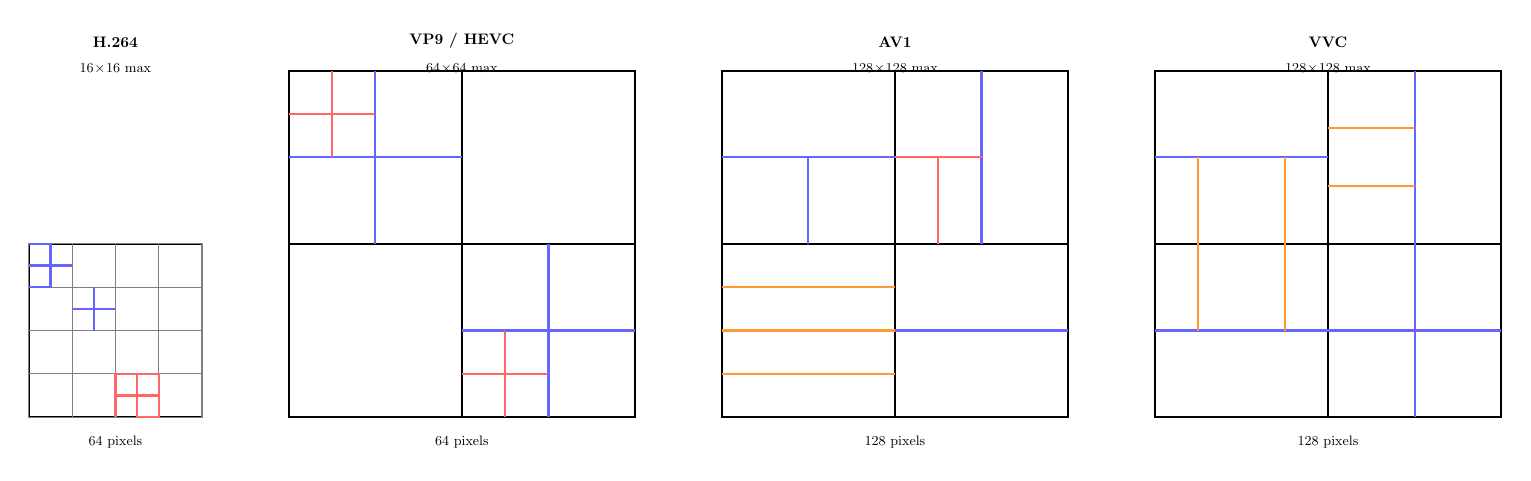
\begin{tikzpicture}[>=Stealth, scale=0.55, every node/.style={scale=0.55}]

% --- H.264 panel ---
\begin{scope}[xshift=0cm]
  \node[font=\normalsize\bfseries, anchor=south] at (2, 8.4) {H.264};
  \node[font=\small, anchor=south] at (2, 7.8) {$16\!\times\!16$ max};
  % 4x4 grid of 16x16 macroblocks in a 64x64 region
  \draw[thick] (0,0) rectangle (4,4);
  \draw[thick] (0,0) rectangle (4,4);
  % macroblock grid
  \foreach \x in {0,1,2,3} {
    \foreach \y in {0,1,2,3} {
      \draw[gray] (\x, \y) rectangle (\x+1, \y+1);
    }
  }
  % show some sub-partitions
  \draw[blue!60, thick] (0,3) -- (0.5,3) -- (0.5,4) -- (0,4);
  \draw[blue!60, thick] (0.5,3) -- (0.5,4);
  \draw[blue!60, thick] (0,3.5) -- (1,3.5);
  % 8x8 in another
  \draw[blue!60, thick] (1,2.5) -- (2,2.5);
  \draw[blue!60, thick] (1.5,2) -- (1.5,3);
  % 4x4 in another
  \draw[red!60, thick] (2,0) -- (2,1) -- (3,1) -- (3,0);
  \draw[red!60, thick] (2.5,0) -- (2.5,0.5);
  \draw[red!60, thick] (2,0.5) -- (2.5,0.5);
  \draw[red!60, thick] (2.5,0.5) -- (2.5,1);
  \draw[red!60, thick] (2.5,0) -- (3,0) -- (3,0.5) -- (2.5,0.5);
  % Scale label
  \node[font=\small, anchor=north] at (2, -0.3) {64 pixels};
\end{scope}

% --- VP9/HEVC panel ---
\begin{scope}[xshift=6cm]
  \node[font=\normalsize\bfseries, anchor=south] at (4, 8.4) {VP9 / HEVC};
  \node[font=\small, anchor=south] at (4, 7.8) {$64\!\times\!64$ max};
  % One 64x64 superblock
  \draw[thick] (0,0) rectangle (8,8);
  % quad-tree splits
  \draw[thick] (4,0) -- (4,8);
  \draw[thick] (0,4) -- (8,4);
  % further splits in top-left quadrant
  \draw[blue!60, thick] (2,4) -- (2,8);
  \draw[blue!60, thick] (0,6) -- (4,6);
  % further split in top-left-top-left
  \draw[red!60, thick] (1,6) -- (1,8);
  \draw[red!60, thick] (0,7) -- (2,7);
  % split bottom-right quadrant
  \draw[blue!60, thick] (6,0) -- (6,4);
  \draw[blue!60, thick] (4,2) -- (8,2);
  % deeper in bottom-right-bottom-left
  \draw[red!60, thick] (5,0) -- (5,2);
  \draw[red!60, thick] (4,1) -- (6,1);
  % Scale label
  \node[font=\small, anchor=north] at (4, -0.3) {64 pixels};
\end{scope}

% --- AV1 panel ---
\begin{scope}[xshift=16cm]
  \node[font=\normalsize\bfseries, anchor=south] at (4, 8.4) {AV1};
  \node[font=\small, anchor=south] at (4, 7.8) {$128\!\times\!128$ max};
  % 128x128 shown as 8x8 grid (each cell = 16px)
  \draw[thick] (0,0) rectangle (8,8);
  % quad split: top half / bottom half
  \draw[thick] (4,0) -- (4,8);
  \draw[thick] (0,4) -- (8,4);
  % rectangular splits in top-left
  \draw[blue!60, thick] (0,6) -- (4,6);
  \draw[blue!60, thick] (2,4) -- (2,6);
  % asymmetric in bottom-left (4:1 rect)
  \draw[orange!80, thick] (0,3) -- (4,3);
  \draw[orange!80, thick] (0,2) -- (4,2);
  \draw[orange!80, thick] (0,1) -- (4,1);
  % quad + rect in top-right
  \draw[blue!60, thick] (6,4) -- (6,8);
  \draw[red!60, thick] (4,6) -- (6,6);
  \draw[red!60, thick] (5,4) -- (5,6);
  % bottom-right: large blocks
  \draw[blue!60, thick] (4,2) -- (8,2);
  % Scale label
  \node[font=\small, anchor=north] at (4, -0.3) {128 pixels};
\end{scope}

% --- VVC panel ---
\begin{scope}[xshift=26cm]
  \node[font=\normalsize\bfseries, anchor=south] at (4, 8.4) {VVC};
  \node[font=\small, anchor=south] at (4, 7.8) {$128\!\times\!128$ max};
  \draw[thick] (0,0) rectangle (8,8);
  % quad split
  \draw[thick] (4,0) -- (4,8);
  \draw[thick] (0,4) -- (8,4);
  % binary split (horizontal) in top-left
  \draw[blue!60, thick] (0,6) -- (4,6);
  % ternary split (vertical) in top-left-bottom
  \draw[orange!80, thick] (1,4) -- (1,6);
  \draw[orange!80, thick] (3,4) -- (3,6);
  % binary split (vertical) in top-right
  \draw[blue!60, thick] (6,4) -- (6,8);
  % ternary horizontal in top-right-left
  \draw[orange!80, thick] (4,5.33) -- (6,5.33);
  \draw[orange!80, thick] (4,6.67) -- (6,6.67);
  % bottom-left: binary horizontal
  \draw[blue!60, thick] (0,2) -- (4,2);
  % deeper ternary in bottom-left-top
  \draw[orange!80, thick] (1,2) -- (1,4);
  \draw[orange!80, thick] (3,2) -- (3,4);
  % bottom-right: mostly large
  \draw[blue!60, thick] (6,0) -- (6,4);
  \draw[blue!60, thick] (4,2) -- (8,2);
  % Scale label
  \node[font=\small, anchor=north] at (4, -0.3) {128 pixels};
\end{scope}

\end{tikzpicture}
\caption{Block partitioning comparison across codec generations. H.264 is
  limited to $16\!\times\!16$ macroblocks with fixed sub-partitions (left).
  VP9/HEVC use quad-tree partitioning within $64\!\times\!64$ superblocks
  (center-left). AV1 extends to $128\!\times\!128$ with quad-tree plus
  rectangular splits (center-right). VVC adds binary and ternary splits for
  maximum flexibility (right). Blue lines show first-level splits; red
  shows deeper partitioning; orange shows asymmetric/ternary splits.}
\label{fig:block-partitioning}
\end{figure}

\begin{table}[ht]
\centering
\small
\renewcommand{\arraystretch}{1.4}
\begin{tabularx}{\textwidth}{lXXXXX}
\toprule
\textbf{Feature} & \textbf{H.264} & \textbf{VP9} & \textbf{HEVC}
  & \textbf{AV1} & \textbf{VVC} \\
\midrule
Max block &
  $16\!\times\!16$ &
  $64\!\times\!64$ &
  $64\!\times\!64$ &
  $128\!\times\!128$ &
  $128\!\times\!128$ \\
Min block &
  $4\!\times\!4$ &
  $4\!\times\!4$ &
  $8\!\times\!8$ &
  $4\!\times\!4$ &
  $4\!\times\!4$ \\
Split types &
  Fixed partitions &
  Quad-tree &
  Quad-tree &
  Quad $+$ rect &
  Quad $+$ BT $+$ TT \\
Asymmetric &
  Limited &
  No &
  No &
  4:1 rectangles &
  Full (BT/TT) \\
\bottomrule
\end{tabularx}
\caption{Block partitioning capabilities by codec. BT = binary tree
  (horizontal or vertical), TT = ternary tree (1:2:1 split). Larger maximum
  blocks reduce overhead for homogeneous regions; asymmetric splits improve
  partitioning efficiency at content boundaries.}
\label{tab:partitioning}
\end{table}

%% ---------------------------------------------------------------------------
\subsection{Rate-Distortion Operating Points by Codec}
\label{sec:rd-comparison}

The codec-specific analyses of
Sections~\ref{sec:mpeg-lineage}--\ref{sec:aom-lineage} can be unified
through the Bj\o ntegaard Delta Rate (BD-Rate), the standard metric for
comparing codec efficiency. BD-Rate computes the average percentage rate
difference between two codecs at equivalent distortion by integrating the
difference between their rate-distortion curves fit as cubic polynomials in
PSNR-vs-log-rate space:
\begin{equation}
  \text{BD-Rate} = \frac{1}{\Delta\text{PSNR}}
    \int_{\text{PSNR}_{\min}}^{\text{PSNR}_{\max}}
    \left[ \ln R_A(p) - \ln R_B(p) \right] dp
  \label{eq:bd-rate}
\end{equation}
A negative BD-Rate indicates that codec~$A$ requires fewer bits than
codec~$B$ at the same quality.

\begin{figure}[ht]
\centering
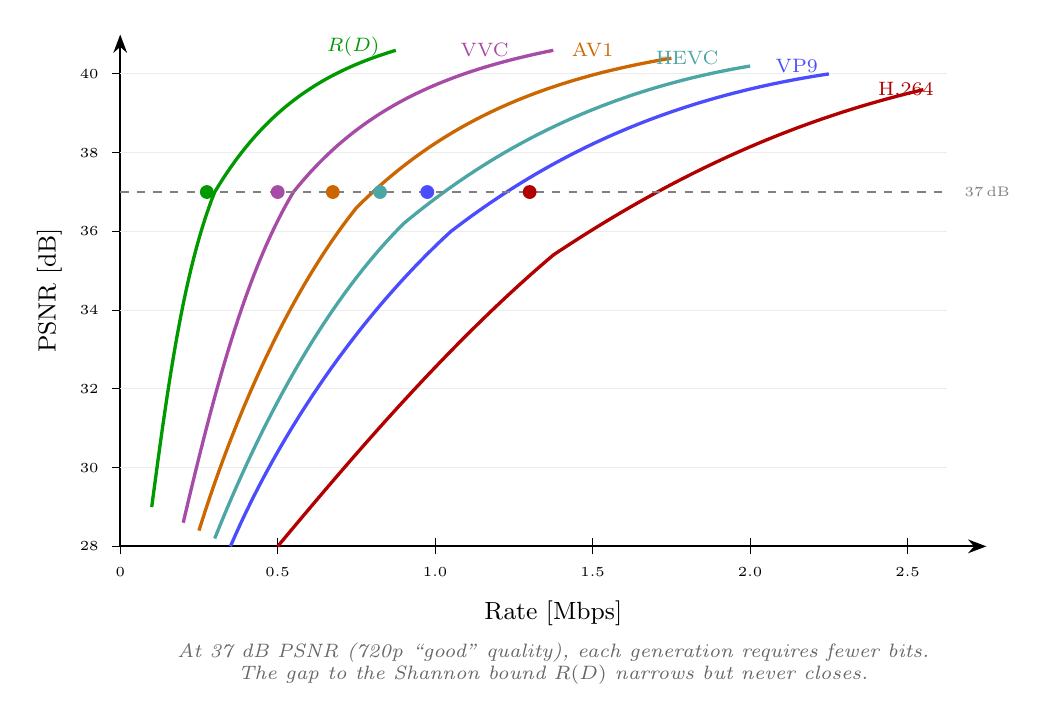
\begin{tikzpicture}[>=Stealth]

% --- Axes ---
\draw[->, thick] (0, 0) -- (11, 0);
\draw[->, thick] (0, 0) -- (0, 6.5);

% --- Axis titles ---
\node[font=\small] at (5.5, -0.85) {Rate [Mbps]};
\node[font=\small, rotate=90] at (-0.9, 3.25) {PSNR [dB]};

% --- X-axis labels ---
\foreach \x/\lab in {0/0, 2/0.5, 4/1.0, 6/1.5, 8/2.0, 10/2.5} {
  \draw (\x, -0.1) -- (\x, 0.1);
  \node[font=\tiny, anchor=north] at (\x, -0.15) {\lab};
}

% --- Y-axis labels ---
\foreach \y/\lab in {0/28, 1/30, 2/32, 3/34, 4/36, 5/38, 6/40} {
  \draw (-0.1, \y) -- (0.1, \y);
  \node[font=\tiny, anchor=east] at (-0.15, \y) {\lab};
}

% --- Grid ---
\foreach \y in {1,2,3,4,5,6} {
  \draw[gray!15] (0, \y) -- (10.5, \y);
}

% --- Shannon R(D) bound (leftmost curve) ---
\draw[very thick, green!60!black]
  (0.4, 0.5) .. controls (0.6, 2) and (0.8, 3.5) ..
  (1.2, 4.5) .. controls (1.8, 5.5) and (2.5, 6.0) ..
  (3.5, 6.3);
\node[font=\scriptsize, green!60!black, anchor=south west] at (2.5, 6.1)
  {$R(D)$};

% --- VVC curve ---
\draw[very thick, violet!70]
  (0.8, 0.3) .. controls (1.2, 2.0) and (1.6, 3.5) ..
  (2.2, 4.5) .. controls (3.0, 5.5) and (4.0, 6.0) ..
  (5.5, 6.3);
\node[font=\scriptsize, violet!70, anchor=south west] at (4.2, 6.1)
  {VVC};

% --- AV1 curve ---
\draw[very thick, orange!80!black]
  (1.0, 0.2) .. controls (1.5, 1.8) and (2.2, 3.3) ..
  (3.0, 4.3) .. controls (4.0, 5.3) and (5.2, 5.9) ..
  (7.0, 6.2);
\node[font=\scriptsize, orange!80!black, anchor=south] at (6.0, 6.1)
  {AV1};

% --- HEVC curve ---
\draw[very thick, teal!70]
  (1.2, 0.1) .. controls (1.8, 1.6) and (2.6, 3.1) ..
  (3.6, 4.1) .. controls (4.8, 5.1) and (6.2, 5.8) ..
  (8.0, 6.1);
\node[font=\scriptsize, teal!70, anchor=south] at (7.2, 6.0)
  {HEVC};

% --- VP9 curve ---
\draw[very thick, blue!70]
  (1.4, 0.0) .. controls (2.0, 1.4) and (3.0, 2.9) ..
  (4.2, 4.0) .. controls (5.5, 5.0) and (7.0, 5.7) ..
  (9.0, 6.0);
\node[font=\scriptsize, blue!70, anchor=south west] at (8.2, 5.9)
  {VP9};

% --- H.264 curve (rightmost) ---
\draw[very thick, red!70!black]
  (2.0, 0.0) .. controls (3.0, 1.2) and (4.2, 2.6) ..
  (5.5, 3.7) .. controls (7.0, 4.7) and (8.5, 5.4) ..
  (10.2, 5.8);
\node[font=\scriptsize, red!70!black, anchor=south west] at (9.5, 5.6)
  {H.264};

% --- 37 dB reference line ---
\draw[thin, gray, dashed] (0, 4.5) -- (10.5, 4.5);
\node[font=\tiny, gray, anchor=west] at (10.6, 4.5) {37\,dB};

% --- Operating points at 37 dB ---
\fill[red!70!black] (5.2, 4.5) circle (2.5pt);
\fill[blue!70] (3.9, 4.5) circle (2.5pt);
\fill[teal!70] (3.3, 4.5) circle (2.5pt);
\fill[orange!80!black] (2.7, 4.5) circle (2.5pt);
\fill[violet!70] (2.0, 4.5) circle (2.5pt);
\fill[green!60!black] (1.1, 4.5) circle (2.5pt);

% --- Annotation ---
\node[font=\scriptsize\itshape, text=black!60, align=center,
  anchor=north] at (5.5, -1.1)
  {At 37~dB PSNR (720p ``good'' quality), each generation
  requires fewer bits.\\
  The gap to the Shannon bound $R(D)$ narrows but never closes.};

\end{tikzpicture}
\caption{Rate-distortion curves for six codecs at 720p/30fps, with the
  Shannon $R(D)$ bound (green). At constant quality (37~dB dashed line),
  the rate progression from H.264 through VVC illustrates the BD-Rate
  savings in Table~\ref{tab:bd-rate}. This figure extends
  Figure~\ref{fig:rate-distortion} from Appendix~\ref{app:info-theory}
  with the full codec lineage.}
\label{fig:rd-curves-detailed}
\end{figure}

\begin{table}[ht]
\centering
\small
\renewcommand{\arraystretch}{1.4}
\begin{tabularx}{\textwidth}{lXXXX}
\toprule
\textbf{Codec} & \textbf{BD-Rate vs.\ H.264}
  & \textbf{$\Delta$ (720p)} & \textbf{Family} & \textbf{Year} \\
\midrule
VP8  & ${\sim}$0\%    & ${\sim}$2.1 & Google    & 2010 \\
VP9  & $-$35\%        & ${\sim}$0.8 & AOM       & 2013 \\
HEVC & $-$40\%        & ${\sim}$0.7 & MPEG/ITU  & 2013 \\
AV1  & $-$54\%        & ${\sim}$0.5 & AOM       & 2018 \\
VVC  & $-$63\%        & ${\sim}$0.3 & MPEG/ITU  & 2020 \\
\bottomrule
\end{tabularx}
\caption{BD-Rate savings and coding efficiency gap $\Delta$
  (eq.~\ref{eq:coding-gap}) for each codec relative to H.264 at 720p/30fps.
  The two families (MPEG/ITU and Google/AOM) achieve comparable efficiency
  within each generation; AV1 slightly trails HEVC, VVC leads AV1 by
  ${\sim}$20\%.}
\label{tab:bd-rate}
\end{table}

Table~\ref{tab:bd-rate} provides the DSP-grounded explanation for the codec
ordering in eq.~(\ref{eq:codec-ordering}) and the savings figures in
eqs.~(\ref{eq:vp9-savings})--(\ref{eq:av1-savings}): each generation adds
tools that reduce $\Delta_{\text{pred}}$, $\Delta_{\text{transform}}$, and
$\Delta_{\text{quant}}$ in (\ref{eq:delta-decomp}), with diminishing
returns as the Shannon bound is approached.

%% ---------------------------------------------------------------------------
\subsection{Scalable Video Coding and Simulcast}
\label{sec:svc-simulcast}

Multi-participant WebRTC sessions require adaptive quality: different
receivers have different bandwidths, and a single encode rate cannot serve
all. Two architectures address this.

\subsubsection{Simulcast}
\label{sec:simulcast}

Simulcast encodes the source at $N$ independent resolution/bitrate
combinations:
\begin{equation}
  R_{\text{simulcast}} = \sum_{i=1}^{N} R_i
  \label{eq:simulcast-rate}
\end{equation}
Each encoding is a fully independent bitstream. A Selective Forwarding
Unit (SFU) selects which stream to forward to each receiver based on
reported bandwidth. The overhead is substantial: a typical 3-layer
simulcast (720p/1.5~Mbps, 360p/500~kbps, 180p/150~kbps) requires
2.15~Mbps total---approximately 1.4$\times$ the cost of the highest
layer alone---with no inter-layer compression benefit.

\subsubsection{Scalable Video Coding (SVC)}
\label{sec:svc}

SVC produces a layered bitstream where a base layer $L_0$ is independently
decodable and enhancement layers $L_1, \ldots, L_K$ refine quality
progressively. Three scalability dimensions exist:

\textbf{Temporal scalability.} The base layer encodes at a reduced frame
rate (e.g., 7.5~fps); enhancement layers add intermediate frames:
\begin{equation}
  R_{\text{temporal}} = R_0 + \sum_{k=1}^{K} \Delta R_k
  \label{eq:temporal-svc}
\end{equation}
where $\Delta R_k \ll R_0$ because enhancement frames reference lower
layers and carry primarily motion-compensated residuals. An SFU drops
enhancement layers for bandwidth-constrained receivers, gracefully
degrading frame rate while preserving spatial quality.

\textbf{Spatial scalability.} The base layer encodes at reduced resolution;
enhancement layers add detail via inter-layer prediction:
\begin{equation}
  R_{\text{spatial}} = R_0 + \Delta R_{\text{upscale}}
  \label{eq:spatial-svc}
\end{equation}
where $\Delta R_{\text{upscale}}$ exploits correlation between the
upsampled base layer and the full-resolution source.

\textbf{Quality (SNR) scalability.} Refinement of quantization at the same
resolution, encoded as the difference between coarse and fine
reconstructions.

SVC achieves 20--30\% rate savings over simulcast for equivalent
adaptivity because enhancement layers exploit inter-layer prediction:
\begin{equation}
  R_{\text{SVC}} < R_{\text{simulcast}} \quad
  \text{(typically by 20--30\%)}
  \label{eq:svc-advantage}
\end{equation}

\begin{figure}[ht]
\centering
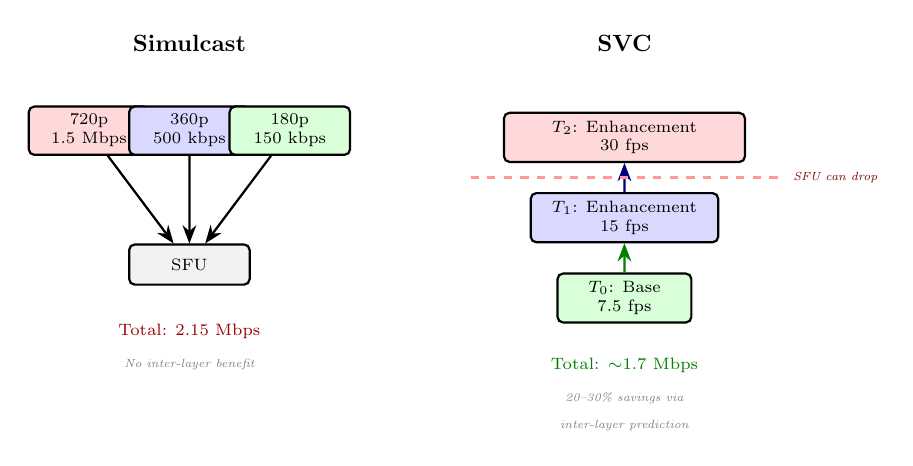
\begin{tikzpicture}[>=Stealth, scale=0.85, every node/.style={scale=0.85},
  layer/.style={draw, rounded corners=2pt, minimum width=1.8cm,
    minimum height=0.6cm, font=\scriptsize, align=center, thick}]

% --- Simulcast (left) ---
\node[font=\normalsize\bfseries] at (2, 5.8) {Simulcast};

% Three independent columns
\node[layer, fill=red!15] (s720) at (0.5, 4.5) {720p\\1.5 Mbps};
\node[layer, fill=blue!15] (s360) at (2.0, 4.5) {360p\\500 kbps};
\node[layer, fill=green!15] (s180) at (3.5, 4.5) {180p\\150 kbps};

\node[layer, fill=gray!10] (sfu1) at (2.0, 2.5) {SFU};

\draw[->, thick] (s720) -- (sfu1);
\draw[->, thick] (s360) -- (sfu1);
\draw[->, thick] (s180) -- (sfu1);

\node[font=\scriptsize, text=red!60!black] at (2.0, 1.5)
  {Total: 2.15 Mbps};
\node[font=\tiny\itshape, text=black!50] at (2.0, 1.0)
  {No inter-layer benefit};

% --- SVC (right) ---
\node[font=\normalsize\bfseries] at (8.5, 5.8) {SVC};

% Pyramid
\node[layer, fill=green!15, minimum width=2.0cm] (t0) at (8.5, 2.0)
  {$T_0$: Base\\7.5 fps};
\node[layer, fill=blue!15, minimum width=2.8cm] (t1) at (8.5, 3.2)
  {$T_1$: Enhancement\\15 fps};
\node[layer, fill=red!15, minimum width=3.6cm] (t2) at (8.5, 4.4)
  {$T_2$: Enhancement\\30 fps};

% Dependency arrows
\draw[->, thick, green!50!black] (t0) -- (t1);
\draw[->, thick, blue!50!black] (t1) -- (t2);

% Drop annotations
\draw[thick, dashed, red!40] (6.2, 3.8) -- (10.8, 3.8);
\node[font=\tiny\itshape, text=red!50!black, anchor=west] at (10.9, 3.8)
  {SFU can drop};

\node[font=\scriptsize, text=green!50!black] at (8.5, 1.0)
  {Total: ${\sim}$1.7 Mbps};
\node[font=\tiny\itshape, text=black!50] at (8.5, 0.5)
  {20--30\% savings via};
\node[font=\tiny\itshape, text=black!50] at (8.5, 0.1)
  {inter-layer prediction};

\end{tikzpicture}
\caption{Simulcast (left) encodes three independent bitstreams with no
  inter-layer compression. SVC (right) encodes a layered bitstream where
  temporal enhancement layers ($T_1$, $T_2$) reference the base layer
  ($T_0$), achieving 20--30\% savings. The SFU drops enhancement layers
  for bandwidth-constrained receivers.}
\label{fig:svc-architecture}
\end{figure}

Codec-specific SVC support relevant to WebRTC:

\begin{itemize}
\item \textbf{H.264 SVC (Annex~G).} Defines temporal, spatial, and quality
  scalability. Complex to implement; rarely used in WebRTC deployments.

\item \textbf{VP9 SVC.} Temporal scalability is widely deployed in WebRTC
  via libvpx (up to 3~temporal layers). Spatial SVC is defined but
  implementation-limited. VP9 temporal SVC is the primary mechanism
  enabling adaptive quality in Chrome/Firefox SFU-based calls.

\item \textbf{AV1 SVC.} Temporal scalability supported in both libaom and
  SVT-AV1. A key enabler for AV1 adoption in production WebRTC
  infrastructure, as SFUs require layered bitstreams to serve heterogeneous
  receivers.
\end{itemize}

Safari's lack of simulcast and SVC support in 2021 (Section~3.1) meant
that Safari users in multi-participant calls could not benefit from adaptive
quality---every receiver got the same stream regardless of bandwidth,
degrading the experience for all participants.

%% ---------------------------------------------------------------------------
\subsection{Hardware vs.\ Software Encoding}
\label{sec:hw-sw}

The main paper identifies hardware encoding as the deployment gate for
AV1 (Sections~8.5, 9.5). This section quantifies why.

\subsubsection{Encoding Complexity}

The computational cost of encoding a video frame is dominated by motion
estimation and RD-optimized mode decision. We express complexity as
operations per pixel:
\begin{equation}
  C_{\text{enc}} = C_{\text{ME}} + C_{\text{transform}}
    + C_{\text{quant}} + C_{\text{entropy}}
    + C_{\text{mode}}
  \label{eq:enc-complexity}
\end{equation}

Representative values for real-time presets:

\begin{itemize}
\item H.264 Constrained Baseline (``veryfast''): $C_{\text{enc}} \approx
  200$~ops/pixel
\item VP9 (speed~8, real-time): $C_{\text{enc}} \approx 600$~ops/pixel
\item AV1 (speed~10, real-time): $C_{\text{enc}} \approx 2000$~ops/pixel
\end{itemize}

The real-time constraint requires:
\begin{equation}
  C_{\text{enc}} \times W \times H \times \text{fps}
    \leq F_{\text{available}}
  \label{eq:realtime-constraint}
\end{equation}
where $F_{\text{available}}$ is the available computational throughput
(operations per second). For 720p/30fps AV1 at 2000~ops/pixel:
\begin{equation}
  2000 \times 921{,}600 \times 30 = 55.3 \times 10^9 \;\text{ops/s}
  \label{eq:av1-cost}
\end{equation}
This consumes approximately one full core of a modern desktop CPU. On
mobile devices with thermal and power constraints, software AV1 encoding
at 720p/30fps remains impractical without hardware acceleration.

\subsubsection{Hardware Encoder Architecture}

Hardware encoders implement a fixed subset of the codec's tool set in
dedicated silicon. The trade-off is quality for throughput: hardware
encoders typically produce output 10--20\% larger than software encoders
at equivalent visual quality because they implement fewer mode decision
candidates and simpler motion search:
\begin{equation}
  \Delta_{\text{HW}} \approx (1.1 \text{--} 1.2)
    \cdot \Delta_{\text{SW}}
  \label{eq:hw-quality-gap}
\end{equation}

This quality penalty is acceptable for real-time communication because:
(a)~the alternative---software encoding at a lower speed preset or reduced
resolution---incurs a larger quality penalty, and (b)~the freed CPU
capacity can be used for pre/post-processing, noise reduction, or
additional application logic.

\subsubsection{Hardware Encoder Availability}

\begin{table}[ht]
\centering
\small
\renewcommand{\arraystretch}{1.4}
\begin{tabularx}{\textwidth}{lXXXX}
\toprule
\textbf{Platform} & \textbf{H.264 HW} & \textbf{VP9 HW encode}
  & \textbf{AV1 HW encode} & \textbf{AV1 year} \\
\midrule
Intel (QSV) &
  Sandy Bridge+ (2011) &
  Kaby Lake+ (2017) &
  Arc / Meteor Lake+ &
  2022 \\
NVIDIA (NVENC) &
  Kepler+ (2012) &
  --- &
  Ada Lovelace+ &
  2022 \\
AMD (VCN) &
  VCN~1.0+ (2017) &
  --- &
  VCN~4.0+ (RDNA~3) &
  2023 \\
Apple (VideoToolbox) &
  A4+ (2010) &
  --- &
  M3+ &
  2023 \\
Qualcomm &
  SD~820+ (2016) &
  --- &
  SD~8 Gen~2+ &
  2023 \\
\bottomrule
\end{tabularx}
\caption{Hardware encoder availability timeline. H.264 hardware encoding
  has been ubiquitous for over a decade. AV1 hardware encoding began
  shipping in 2022--2023 across all major platforms; the main paper projects
  it becomes the practical WebRTC default by 2028--2030 as these chipsets
  reach market saturation.}
\label{tab:hw-encoders}
\end{table}

\excursus{Excursus: WebCodecs and hardware acceleration.}{When a WebCodecs
\texttt{VideoEncoder} is configured with \texttt{codec: "av01"}, the browser
selects hardware or software encoding based on platform capability and the
\texttt{hardwareAcceleration} preference (\texttt{"prefer-hardware"},
\texttt{"prefer-software"}, or \texttt{"no-preference"}). The application
receives encoded \texttt{EncodedVideoChunk} objects either way, but latency
and CPU cost differ dramatically: hardware encoding typically adds
$<\!1$~ms per frame and consumes near-zero CPU, while software AV1 at
real-time presets consumes an entire CPU core
(eq.~\ref{eq:av1-cost}). This abstraction is what makes the hardware
timeline in Table~\ref{tab:hw-encoders} directly relevant to the WebCodecs
adoption curve in Section~7.}

The hardware encoding timeline directly underpins the main paper's
projections: the ``AV1 becomes practical'' milestone (Section~8.5) and
``AV1 HW ubiquitous'' milestone (Section~9.5) depend on the chipset
generations in Table~\ref{tab:hw-encoders} reaching market saturation.

%% ---------------------------------------------------------------------------
\subsection{Implications for Real-Time Web Communication}
\label{sec:video-implications}

The DSP analysis of this appendix maps back to concrete implications for
the technologies surveyed in the main text.

\textbf{The hybrid coding framework is universal; innovation is
incremental.} Every codec from VP8 to VVC implements the same
prediction--transform--quantization--entropy framework
(Figure~\ref{fig:hybrid-encoder}). Generational improvements come from
expanding the tool set within this framework---more block sizes
(Table~\ref{tab:partitioning}), more prediction modes, more transform
types (Table~\ref{tab:transforms})---not from fundamentally new
architectures. This means the efficiency gap $\Delta$ approaches but never
reaches zero: each additional tool yields diminishing rate-distortion
improvement at increasing computational cost.

\textbf{Transform and prediction innovations explain the BD-Rate
progression.} The 35\% rate saving from H.264 to VP9 comes primarily from
larger blocks ($64\!\times\!64$ vs.\ $16\!\times\!16$) and adaptive
transforms (DCT$+$ADST vs.\ fixed DCT). The additional 30\% from VP9 to
AV1 comes from compound and warped motion, film grain synthesis, and
16-way transform type selection (Table~\ref{tab:bd-rate}). Each tool adds
encoding complexity proportional to its rate-distortion benefit, which is
why real-time encoders must aggressively prune the tool set.

\textbf{SVC is what makes multi-participant WebRTC work.} Without temporal
SVC, an SFU must forward full-rate streams to all participants regardless
of their bandwidth. With VP9/AV1 temporal SVC
(Section~\ref{sec:svc}), the SFU drops enhancement temporal layers for
bandwidth-constrained receivers, degrading frame rate gracefully while
preserving spatial quality. The 20--30\% savings over simulcast
(eq.~\ref{eq:svc-advantage}) translate directly to reduced server egress
bandwidth in large meetings.

\textbf{Hardware encoding is the deployment gate, not codec specification.}
AV1 was specified in 2018 but becomes a practical WebRTC default only
when hardware encoders are ubiquitous (${\sim}$2028--2030). The DSP tools
that make AV1 efficient---warped motion, OBMC, $128\!\times\!128$
superblocks with flexible partitioning---are precisely the tools that make
it computationally expensive in software (eq.~\ref{eq:av1-cost}). The
${\sim}$10--20\% quality penalty of hardware encoders
(eq.~\ref{eq:hw-quality-gap}) is the price of real-time feasibility, and
it is a price worth paying: $\Delta_{\text{AV1,HW}} \approx 0.6$ is still
far below $\Delta_{\text{VP9,SW}} \approx 0.8$.

\textbf{The convergence toward Shannon is real but asymptotic.}
Cross-referencing with Appendix~\ref{app:info-theory}: H.264's
$\Delta \approx 2.1$ means it operates at $3.1\times$ the theoretical
minimum rate. VP9's $\Delta \approx 0.8$ means $1.8\times$. AV1's
$\Delta \approx 0.5$ means $1.5\times$. VVC's $\Delta \approx 0.3$ means
$1.3\times$. Each generation captures more spatial, temporal, and
perceptual redundancy, but the returns are diminishing: the distance from
H.264 to VP9 ($-$35\%) exceeds VP9 to AV1 ($-$30\%), which exceeds AV1 to
VVC ($-$17\%). The next generation of efficiency gains for real-time web
communication will come not from codecs alone, but from the co-optimization
of transport (QUIC, WebTransport), application architecture (WebCodecs,
unbundled pipelines), and network infrastructure that the main text
describes.


\end{document}
